% Options for packages loaded elsewhere
\PassOptionsToPackage{unicode}{hyperref}
\PassOptionsToPackage{hyphens}{url}
\PassOptionsToPackage{dvipsnames,svgnames,x11names}{xcolor}
%
\documentclass[
  letterpaper,
  DIV=11,
  numbers=noendperiod]{scrreprt}

\usepackage{amsmath,amssymb}
\usepackage{iftex}
\ifPDFTeX
  \usepackage[T1]{fontenc}
  \usepackage[utf8]{inputenc}
  \usepackage{textcomp} % provide euro and other symbols
\else % if luatex or xetex
  \usepackage{unicode-math}
  \defaultfontfeatures{Scale=MatchLowercase}
  \defaultfontfeatures[\rmfamily]{Ligatures=TeX,Scale=1}
\fi
\usepackage{lmodern}
\ifPDFTeX\else  
    % xetex/luatex font selection
\fi
% Use upquote if available, for straight quotes in verbatim environments
\IfFileExists{upquote.sty}{\usepackage{upquote}}{}
\IfFileExists{microtype.sty}{% use microtype if available
  \usepackage[]{microtype}
  \UseMicrotypeSet[protrusion]{basicmath} % disable protrusion for tt fonts
}{}
\makeatletter
\@ifundefined{KOMAClassName}{% if non-KOMA class
  \IfFileExists{parskip.sty}{%
    \usepackage{parskip}
  }{% else
    \setlength{\parindent}{0pt}
    \setlength{\parskip}{6pt plus 2pt minus 1pt}}
}{% if KOMA class
  \KOMAoptions{parskip=half}}
\makeatother
\usepackage{xcolor}
\setlength{\emergencystretch}{3em} % prevent overfull lines
\setcounter{secnumdepth}{5}
% Make \paragraph and \subparagraph free-standing
\makeatletter
\ifx\paragraph\undefined\else
  \let\oldparagraph\paragraph
  \renewcommand{\paragraph}{
    \@ifstar
      \xxxParagraphStar
      \xxxParagraphNoStar
  }
  \newcommand{\xxxParagraphStar}[1]{\oldparagraph*{#1}\mbox{}}
  \newcommand{\xxxParagraphNoStar}[1]{\oldparagraph{#1}\mbox{}}
\fi
\ifx\subparagraph\undefined\else
  \let\oldsubparagraph\subparagraph
  \renewcommand{\subparagraph}{
    \@ifstar
      \xxxSubParagraphStar
      \xxxSubParagraphNoStar
  }
  \newcommand{\xxxSubParagraphStar}[1]{\oldsubparagraph*{#1}\mbox{}}
  \newcommand{\xxxSubParagraphNoStar}[1]{\oldsubparagraph{#1}\mbox{}}
\fi
\makeatother

\usepackage{color}
\usepackage{fancyvrb}
\newcommand{\VerbBar}{|}
\newcommand{\VERB}{\Verb[commandchars=\\\{\}]}
\DefineVerbatimEnvironment{Highlighting}{Verbatim}{commandchars=\\\{\}}
% Add ',fontsize=\small' for more characters per line
\usepackage{framed}
\definecolor{shadecolor}{RGB}{241,243,245}
\newenvironment{Shaded}{\begin{snugshade}}{\end{snugshade}}
\newcommand{\AlertTok}[1]{\textcolor[rgb]{0.68,0.00,0.00}{#1}}
\newcommand{\AnnotationTok}[1]{\textcolor[rgb]{0.37,0.37,0.37}{#1}}
\newcommand{\AttributeTok}[1]{\textcolor[rgb]{0.40,0.45,0.13}{#1}}
\newcommand{\BaseNTok}[1]{\textcolor[rgb]{0.68,0.00,0.00}{#1}}
\newcommand{\BuiltInTok}[1]{\textcolor[rgb]{0.00,0.23,0.31}{#1}}
\newcommand{\CharTok}[1]{\textcolor[rgb]{0.13,0.47,0.30}{#1}}
\newcommand{\CommentTok}[1]{\textcolor[rgb]{0.37,0.37,0.37}{#1}}
\newcommand{\CommentVarTok}[1]{\textcolor[rgb]{0.37,0.37,0.37}{\textit{#1}}}
\newcommand{\ConstantTok}[1]{\textcolor[rgb]{0.56,0.35,0.01}{#1}}
\newcommand{\ControlFlowTok}[1]{\textcolor[rgb]{0.00,0.23,0.31}{\textbf{#1}}}
\newcommand{\DataTypeTok}[1]{\textcolor[rgb]{0.68,0.00,0.00}{#1}}
\newcommand{\DecValTok}[1]{\textcolor[rgb]{0.68,0.00,0.00}{#1}}
\newcommand{\DocumentationTok}[1]{\textcolor[rgb]{0.37,0.37,0.37}{\textit{#1}}}
\newcommand{\ErrorTok}[1]{\textcolor[rgb]{0.68,0.00,0.00}{#1}}
\newcommand{\ExtensionTok}[1]{\textcolor[rgb]{0.00,0.23,0.31}{#1}}
\newcommand{\FloatTok}[1]{\textcolor[rgb]{0.68,0.00,0.00}{#1}}
\newcommand{\FunctionTok}[1]{\textcolor[rgb]{0.28,0.35,0.67}{#1}}
\newcommand{\ImportTok}[1]{\textcolor[rgb]{0.00,0.46,0.62}{#1}}
\newcommand{\InformationTok}[1]{\textcolor[rgb]{0.37,0.37,0.37}{#1}}
\newcommand{\KeywordTok}[1]{\textcolor[rgb]{0.00,0.23,0.31}{\textbf{#1}}}
\newcommand{\NormalTok}[1]{\textcolor[rgb]{0.00,0.23,0.31}{#1}}
\newcommand{\OperatorTok}[1]{\textcolor[rgb]{0.37,0.37,0.37}{#1}}
\newcommand{\OtherTok}[1]{\textcolor[rgb]{0.00,0.23,0.31}{#1}}
\newcommand{\PreprocessorTok}[1]{\textcolor[rgb]{0.68,0.00,0.00}{#1}}
\newcommand{\RegionMarkerTok}[1]{\textcolor[rgb]{0.00,0.23,0.31}{#1}}
\newcommand{\SpecialCharTok}[1]{\textcolor[rgb]{0.37,0.37,0.37}{#1}}
\newcommand{\SpecialStringTok}[1]{\textcolor[rgb]{0.13,0.47,0.30}{#1}}
\newcommand{\StringTok}[1]{\textcolor[rgb]{0.13,0.47,0.30}{#1}}
\newcommand{\VariableTok}[1]{\textcolor[rgb]{0.07,0.07,0.07}{#1}}
\newcommand{\VerbatimStringTok}[1]{\textcolor[rgb]{0.13,0.47,0.30}{#1}}
\newcommand{\WarningTok}[1]{\textcolor[rgb]{0.37,0.37,0.37}{\textit{#1}}}

\providecommand{\tightlist}{%
  \setlength{\itemsep}{0pt}\setlength{\parskip}{0pt}}\usepackage{longtable,booktabs,array}
\usepackage{calc} % for calculating minipage widths
% Correct order of tables after \paragraph or \subparagraph
\usepackage{etoolbox}
\makeatletter
\patchcmd\longtable{\par}{\if@noskipsec\mbox{}\fi\par}{}{}
\makeatother
% Allow footnotes in longtable head/foot
\IfFileExists{footnotehyper.sty}{\usepackage{footnotehyper}}{\usepackage{footnote}}
\makesavenoteenv{longtable}
\usepackage{graphicx}
\makeatletter
\newsavebox\pandoc@box
\newcommand*\pandocbounded[1]{% scales image to fit in text height/width
  \sbox\pandoc@box{#1}%
  \Gscale@div\@tempa{\textheight}{\dimexpr\ht\pandoc@box+\dp\pandoc@box\relax}%
  \Gscale@div\@tempb{\linewidth}{\wd\pandoc@box}%
  \ifdim\@tempb\p@<\@tempa\p@\let\@tempa\@tempb\fi% select the smaller of both
  \ifdim\@tempa\p@<\p@\scalebox{\@tempa}{\usebox\pandoc@box}%
  \else\usebox{\pandoc@box}%
  \fi%
}
% Set default figure placement to htbp
\def\fps@figure{htbp}
\makeatother

\KOMAoption{captions}{tableheading}
\makeatletter
\@ifpackageloaded{bookmark}{}{\usepackage{bookmark}}
\makeatother
\makeatletter
\@ifpackageloaded{caption}{}{\usepackage{caption}}
\AtBeginDocument{%
\ifdefined\contentsname
  \renewcommand*\contentsname{Tabla de contenidos}
\else
  \newcommand\contentsname{Tabla de contenidos}
\fi
\ifdefined\listfigurename
  \renewcommand*\listfigurename{Listado de Figuras}
\else
  \newcommand\listfigurename{Listado de Figuras}
\fi
\ifdefined\listtablename
  \renewcommand*\listtablename{Listado de Tablas}
\else
  \newcommand\listtablename{Listado de Tablas}
\fi
\ifdefined\figurename
  \renewcommand*\figurename{Figura}
\else
  \newcommand\figurename{Figura}
\fi
\ifdefined\tablename
  \renewcommand*\tablename{Tabla}
\else
  \newcommand\tablename{Tabla}
\fi
}
\@ifpackageloaded{float}{}{\usepackage{float}}
\floatstyle{ruled}
\@ifundefined{c@chapter}{\newfloat{codelisting}{h}{lop}}{\newfloat{codelisting}{h}{lop}[chapter]}
\floatname{codelisting}{Listado}
\newcommand*\listoflistings{\listof{codelisting}{Listado de Listados}}
\makeatother
\makeatletter
\makeatother
\makeatletter
\@ifpackageloaded{caption}{}{\usepackage{caption}}
\@ifpackageloaded{subcaption}{}{\usepackage{subcaption}}
\makeatother

\ifLuaTeX
\usepackage[bidi=basic]{babel}
\else
\usepackage[bidi=default]{babel}
\fi
\babelprovide[main,import]{spanish}
% get rid of language-specific shorthands (see #6817):
\let\LanguageShortHands\languageshorthands
\def\languageshorthands#1{}
\usepackage{bookmark}

\IfFileExists{xurl.sty}{\usepackage{xurl}}{} % add URL line breaks if available
\urlstyle{same} % disable monospaced font for URLs
\hypersetup{
  pdftitle={ApLabAD},
  pdfauthor={RICUIB},
  pdflang={es},
  colorlinks=true,
  linkcolor={blue},
  filecolor={Maroon},
  citecolor={Blue},
  urlcolor={Blue},
  pdfcreator={LaTeX via pandoc}}


\title{ApLabAD}
\usepackage{etoolbox}
\makeatletter
\providecommand{\subtitle}[1]{% add subtitle to \maketitle
  \apptocmd{\@title}{\par {\large #1 \par}}{}{}
}
\makeatother
\subtitle{Apuntes de Laboratorio de Análisis de Datos}
\author{RICUIB}
\date{2025-02-01}

\begin{document}
\maketitle

\renewcommand*\contentsname{Tabla de contenidos}
{
\hypersetup{linkcolor=}
\setcounter{tocdepth}{2}
\tableofcontents
}

\bookmarksetup{startatroot}

\chapter*{Prefacio}\label{prefacio}
\addcontentsline{toc}{chapter}{Prefacio}

\markboth{Prefacio}{Prefacio}

Este libro en la web es una versión de las notas de clase de asignaturas
introductorias al análisis de datos.

\begin{description}
\item[Ha sido elaborado con \href{https://quarto.org/}{Quarto}]
RStudio, PBC. (2022). Quarto (Version 1.0). Hemos utilizado el formato
formato book.
\end{description}

¿Quarto book o bookdown?
\url{https://yihui.org/en/2022/04/quarto-r-markdown/}

\part{Parte 1: Probabilidad y variables aleatorias}

En esta sección, veremos la teoría básica de la probabilidad y de las
variables aleatorias. Resolveremos problemas prácticos para comprender
mejor los conceptos y utilizaremos R para realizar cálculos y gráficos.

También exploraremos los modelos de probabilidad discretos y continuos
más conocidos.

En ocasiones, trabajaremos con problemas de cálculo más complejos.

Además, introduciremos problemas sencillos de modelización con
probabilidades. Estos consistirán en un enunciado, real o inventado, en
el que se pedirá modelizar el problema mediante una variable aleatoria y
responder a una serie de preguntas.

\chapter{Preliminares: conjuntos y
combinatoria}\label{preliminares-conjuntos-y-combinatoria}

Para aprender cálculo de probabilidades son necesarios conocimientos de:

\begin{enumerate}
\def\labelenumi{\arabic{enumi}.}
\tightlist
\item
  Cálculo: Derivadas, integrales, límites, sumas de series\ldots{}
\item
  Geometría básica y álgebra lineal : rectas, hiperplanos,
  volúmenes\ldots{} Matrices, valores propios\ldots{}
\item
  Teoría de conjuntos y combinatoria\ldots..
\end{enumerate}

Por experiencia sabemos que la mayoría de estudiantes tienen más
conocimientos de cálculo, geometría y matrices.

Pero muchos tienen una falta de conocimientos en teoría básica de
conjuntos y combinatoria (matemática discreta).

\section{Teoría de conjuntos}\label{teoruxeda-de-conjuntos}

Definición de conjunto

La definición de conjunto es una
\href{https://es.wikipedia.org/wiki/Concepto_primitivo}{idea o noción
primitiva}. Es decir es una idea básica del pensamiento humano: un
conjunto es una colección de objetos: números, imágenes\ldots{}
cualquier cosa, jugadores de fútbol, palabras, colores \ldots.

La definición de conjunto es una
\href{https://es.wikipedia.org/wiki/Concepto_primitivo}{idea o noción
primitiva}. Es decir es una idea básica del pensamiento humano: un
conjunto es una colección de objetos: números, imágenes\ldots{}
cualquier cosa, jugadores de fútbol, palabras, colores \ldots.

La teoría de conjuntos básicas es simple y natural y es la que
necesitamos para este curso.

La teoría de conjuntos matemática es más compleja y presenta varias
paradojas como la
\href{https://es.wikipedia.org/wiki/Paradoja_de_Russell}{paradoja de
Russell}.

La idea o noción práctica de conjunto es la de una colección de objetos
de un cierto tipo.

Estas colecciones o conjuntos se pueden definir por:

\begin{itemize}
\tightlist
\item
  \textbf{Comprensión}: reuniendo los objetos que cumplen una propiedad
  \(p\)
\item
  \textbf{Extensión}: dando una lista exhaustiva de los miembros del
  conjunto
\end{itemize}

\subsection{Conjuntos básicos}\label{conjuntos-buxe1sicos}

Los conjuntos suelen tener un conjunto madre como por ejemplo

\begin{itemize}
\item
  \(\mathbb{N}=\{0,1,2,\ldots\}\)
\item
  \(\mathbb{Z}=\{\ldots,-2,-1,0,1,2,\ldots\}\)
\item
  \(\mathbb{Q}=\left\{\frac{p}{q}\quad\Big|\quad p,q\in \mathbb{Z} \mbox{ y } q \not= 0.\right\}\)
\item
  \(\mathbb{R}=\{\mbox{Todos los puntos de una recta.}\}\)
\item
  \(\mathbb{C}= \left\{a+b\cdot i\quad \big|\quad a,b\in \mathbb{R}\right\}\mbox{ los números complejos}\quad a+b\cdot i.\)
\item
  Alfabeto = \(\{a,b,c,\ldots, A,B,C,\ldots\}.\)
\item
  Palabras = \(\{paz, guerra, amor, probabilidad,\ldots\}.\)
\end{itemize}

Recordemos que \(i\) es la unidad imaginaria que cumple que
\(i=\sqrt{-1}\).

\subsection{Características y propiedades básicas de los
conjuntos}\label{caracteruxedsticas-y-propiedades-buxe1sicas-de-los-conjuntos}

Si a cada objeto \(x\) de \(\Omega\) le llamaremos \textbf{elemento del
conjunto} \(\Omega\) y diremos que \(x\) pertenece a \(\Omega\). Lo
denotaremos por \(x\in \Omega\).

Un \textbf{conjunto de un elemento}, por ejemplo \(\{1\}\) recibe el
nombre de \textbf{conjunto elemental} (o \textbf{singleton} del inglés).

Sea \(A\) otro conjunto diremos que \(A\) \textbf{es igual a} \(B\) si
todos los elementos \(A\) están en \(B\) y todos los elementos de \(B\)
están en \(A\). Por ejemplo \(A=\{1,2,3\}\) es igual a \(B=\{3,1,2\}\).

Si \(B\) es otro conjunto, tal que si \(x\in A\) entonces \(x\in B\)
diremos que \(A\) es un subconjunto de o que está contenido en \(B\). Lo
denotaremos por \(A\subseteq B.\)

El conjunto que no tiene elementos se denomina conjunto vacío y se
denota por el símbolo \(\emptyset\). Dado \(A\) un conjunto cualquiera
obviamente \(\emptyset\subseteq A.\)

Ejemplo

Tomemos como conjunto base \(\Omega=\{1,2,3\}\)

\begin{itemize}
\tightlist
\item
  \(\Omega\) es un conjunto de cardinal 3, se denota por
  \(\#(\Omega)=3\) o por \(|\Omega|=3\)
\item
  El conjunto \(\Omega\) tiene \(2^3=8\) subconjuntos.

  \begin{itemize}
  \tightlist
  \item
    el vacío \(\emptyset\) y los elementales \(\{1\},\{2\},\{3\}\)
  \item
    los subconjuntos de dos elementos: \(\{1,2\},\{1,3\},\{2,3\}\)
  \item
    el conjunto total de tres elementos \(\Omega=\{1,2,3\}.\)
  \end{itemize}
\end{itemize}

Dado un conjunto \(\Omega\) podemos construir el \textbf{conjunto de
todas sus partes} (todos sus subconjuntos) al que denotamos por
\(\mathcal{P}(\Omega)\). También se denomina de forma directa partes de
\(\Omega\).

Cardinal de las partes de un conjunto

Propiedad

Por ejemplo
\(\#\left(\mathcal{P}(\{1,2,3\})\right)=2^{\#(\{1,2,3\})}=2^3=8.\)

Efectivamente

\[\mathcal{P}(\{1,2,3\})=\{\emptyset,\{1\},\{2\},\{3\},\{1,2\},\{1,3\},\{2,3\},\{1,2,3\}\}.\]

Dado un subconjunto \(A\) de \(\Omega\) podemos construir la función
característica de \(A\) \[\chi_A:\Omega \to \{0,1\}\]

dado un \(\omega\in \Omega\)

\[
\chi_A(\omega)=
\left\{
\begin{array}{ll}
1 &  \mbox{si }\omega \in A\\
0 &  \mbox{si }\omega \not\in A
\end{array}
\right.
\]

\subsection{Operaciones entre
conjuntos}\label{operaciones-entre-conjuntos}

\textbf{Intersección}

Sea \(\Omega\) un conjunto y \(A\) y \(B\) dos subconjuntos de
\(\Omega\).

El conjunto \textbf{intersección} de \(A\) y \(B\) es el formado por
todos los elementos que perteneces a \(A\) \textbf{Y} \(B\), se denota
por \(A\cap B\).

Más formalmente

\[
A\cap B=\left\{x\in\Omega \big| x\in A \mbox{ y } x\in B\right\}.
\]

\textbf{Unión}

El conjunto \textbf{unión} de \(A\) y \(B\) es el formado por todos los
elementos que perteneces a \(A\) \textbf{O} pertenecen a \(B\), se
denota por \(A\cup B\).

Más formalmente

\[
A\cup B=\left\{x\in\Omega \big| x\in A \mbox{ o } x\in B\right\}.
\]

Diferencia.

El conjunto \textbf{diferencia} de \(A\) y \(B\) es el formado por todos
los elementos que perteneces a \(A\) \textbf{Y NO} pertenecen a \(B\),
se denota por \(A-B=A-(A\cap B)\).

Más formalmente

\[
A- B=\left\{x\in\Omega \big| x\in A \mbox{ y } x\notin B\right\}.
\]

Complementario

El \textbf{complementario} de un subconjunto \(A\) de \(\Omega\) es
\(\Omega-A\) y se denota por \(A^c\) o \(\overline{A}\).

Más formalmente

\[
A^c=\left\{x\in\Omega \big| x\not\in A\right\}.
\]

\subsection{Más propiedades}\label{muxe1s-propiedades}

Sea \(\Omega\) un conjunto y \(A\), \(B\), \(C\) tres subconjuntos de
\(\Omega\)

\begin{itemize}
\tightlist
\item
  Se dice que dos conjuntos \(A\) y \(B\) \textbf{son disjuntos} si
  \(A\cap B=\emptyset.\)
\item
  \(\Omega^c=\emptyset\).
\item
  \(\emptyset^c=\Omega\).
\item
  \(A\cup B=B \cup A\) , \(A\cap B=B\cap A\) conmutativas.
\item
  \((A\cup B) \cup C = A \cup( B \cup C)\),
  \((A\cap B) \cap C = A \cap( B \cap C)\) asociativas.
\item
  \(A\cup (B\cap C)=(A\cup B) \cap (A\cup C)\),
  \(A\cap (B\cup C)=(A\cap B) \cup (A\cap C)\) distributivas.
\item
  \(\left(A^c\right)^c=A\) doble complementario.
\item
  \(\left(A\cup B\right)^c=A^c \cap B^c\),
  \(\left(A\cap B\right)^c=A^c \cup B^c\)
  \href{https://es.wikipedia.org/wiki/Leyes_de_De_Morgan}{leyes de De
  Morgan}.
\end{itemize}

\subsection{Con R, ejemplos.}\label{con-r-ejemplos.}

Con R los conjuntos de pueden definir como vectores

\begin{Shaded}
\begin{Highlighting}[]
\NormalTok{Omega}\OtherTok{=}\FunctionTok{c}\NormalTok{(}\DecValTok{1}\NormalTok{,}\DecValTok{2}\NormalTok{,}\DecValTok{3}\NormalTok{,}\DecValTok{4}\NormalTok{,}\DecValTok{5}\NormalTok{,}\DecValTok{6}\NormalTok{,}\DecValTok{7}\NormalTok{,}\DecValTok{8}\NormalTok{,}\DecValTok{9}\NormalTok{,}\DecValTok{10}\NormalTok{)}
\NormalTok{A}\OtherTok{=}\FunctionTok{c}\NormalTok{(}\DecValTok{1}\NormalTok{,}\DecValTok{2}\NormalTok{,}\DecValTok{3}\NormalTok{,}\DecValTok{4}\NormalTok{,}\DecValTok{5}\NormalTok{)}
\NormalTok{B}\OtherTok{=}\FunctionTok{c}\NormalTok{(}\DecValTok{1}\NormalTok{,}\DecValTok{4}\NormalTok{,}\DecValTok{5}\NormalTok{)}
\NormalTok{C}\OtherTok{=}\FunctionTok{c}\NormalTok{(}\DecValTok{4}\NormalTok{,}\DecValTok{6}\NormalTok{,}\DecValTok{7}\NormalTok{,}\DecValTok{8}\NormalTok{)}
\NormalTok{Omega}
\end{Highlighting}
\end{Shaded}

\begin{verbatim}
 [1]  1  2  3  4  5  6  7  8  9 10
\end{verbatim}

\begin{Shaded}
\begin{Highlighting}[]
\NormalTok{A}
\end{Highlighting}
\end{Shaded}

\begin{verbatim}
[1] 1 2 3 4 5
\end{verbatim}

\begin{Shaded}
\begin{Highlighting}[]
\NormalTok{B}
\end{Highlighting}
\end{Shaded}

\begin{verbatim}
[1] 1 4 5
\end{verbatim}

\begin{Shaded}
\begin{Highlighting}[]
\NormalTok{C}
\end{Highlighting}
\end{Shaded}

\begin{verbatim}
[1] 4 6 7 8
\end{verbatim}

\(A\cap B\)

\begin{Shaded}
\begin{Highlighting}[]
\NormalTok{A}
\end{Highlighting}
\end{Shaded}

\begin{verbatim}
[1] 1 2 3 4 5
\end{verbatim}

\begin{Shaded}
\begin{Highlighting}[]
\NormalTok{B}
\end{Highlighting}
\end{Shaded}

\begin{verbatim}
[1] 1 4 5
\end{verbatim}

\begin{Shaded}
\begin{Highlighting}[]
\FunctionTok{intersect}\NormalTok{(A,B)}
\end{Highlighting}
\end{Shaded}

\begin{verbatim}
[1] 1 4 5
\end{verbatim}

\(A\cup B\)

\begin{Shaded}
\begin{Highlighting}[]
\NormalTok{A}
\end{Highlighting}
\end{Shaded}

\begin{verbatim}
[1] 1 2 3 4 5
\end{verbatim}

\begin{Shaded}
\begin{Highlighting}[]
\NormalTok{B}
\end{Highlighting}
\end{Shaded}

\begin{verbatim}
[1] 1 4 5
\end{verbatim}

\begin{Shaded}
\begin{Highlighting}[]
\FunctionTok{union}\NormalTok{(A,B)}
\end{Highlighting}
\end{Shaded}

\begin{verbatim}
[1] 1 2 3 4 5
\end{verbatim}

\(B-C\)

\begin{Shaded}
\begin{Highlighting}[]
\NormalTok{B}
\end{Highlighting}
\end{Shaded}

\begin{verbatim}
[1] 1 4 5
\end{verbatim}

\begin{Shaded}
\begin{Highlighting}[]
\NormalTok{C}
\end{Highlighting}
\end{Shaded}

\begin{verbatim}
[1] 4 6 7 8
\end{verbatim}

\begin{Shaded}
\begin{Highlighting}[]
\FunctionTok{setdiff}\NormalTok{(B,C)}
\end{Highlighting}
\end{Shaded}

\begin{verbatim}
[1] 1 5
\end{verbatim}

\(A^c=\Omega-A\)

\begin{Shaded}
\begin{Highlighting}[]
\NormalTok{Omega}
\end{Highlighting}
\end{Shaded}

\begin{verbatim}
 [1]  1  2  3  4  5  6  7  8  9 10
\end{verbatim}

\begin{Shaded}
\begin{Highlighting}[]
\NormalTok{A}
\end{Highlighting}
\end{Shaded}

\begin{verbatim}
[1] 1 2 3 4 5
\end{verbatim}

\begin{Shaded}
\begin{Highlighting}[]
\FunctionTok{setdiff}\NormalTok{(Omega,A)}
\end{Highlighting}
\end{Shaded}

\begin{verbatim}
[1]  6  7  8  9 10
\end{verbatim}

\subsection{Con python}\label{con-python}

\begin{Shaded}
\begin{Highlighting}[]
\NormalTok{Omega}\OperatorTok{=}\BuiltInTok{set}\NormalTok{([}\DecValTok{1}\NormalTok{,}\DecValTok{2}\NormalTok{,}\DecValTok{3}\NormalTok{,}\DecValTok{4}\NormalTok{,}\DecValTok{5}\NormalTok{,}\DecValTok{6}\NormalTok{,}\DecValTok{7}\NormalTok{,}\DecValTok{8}\NormalTok{,}\DecValTok{9}\NormalTok{,}\DecValTok{10}\NormalTok{])}
\NormalTok{A}\OperatorTok{=}\BuiltInTok{set}\NormalTok{([}\DecValTok{1}\NormalTok{,}\DecValTok{2}\NormalTok{,}\DecValTok{3}\NormalTok{,}\DecValTok{4}\NormalTok{,}\DecValTok{5}\NormalTok{])}
\NormalTok{B}\OperatorTok{=}\BuiltInTok{set}\NormalTok{([}\DecValTok{1}\NormalTok{,}\DecValTok{4}\NormalTok{,}\DecValTok{5}\NormalTok{])}
\NormalTok{C}\OperatorTok{=}\BuiltInTok{set}\NormalTok{([}\DecValTok{4}\NormalTok{,}\DecValTok{6}\NormalTok{,}\DecValTok{7}\NormalTok{,}\DecValTok{8}\NormalTok{])}
\NormalTok{Omega}
\end{Highlighting}
\end{Shaded}

\begin{verbatim}
{1, 2, 3, 4, 5, 6, 7, 8, 9, 10}
\end{verbatim}

\begin{Shaded}
\begin{Highlighting}[]
\NormalTok{A}
\end{Highlighting}
\end{Shaded}

\begin{verbatim}
{1, 2, 3, 4, 5}
\end{verbatim}

\begin{Shaded}
\begin{Highlighting}[]
\NormalTok{B}
\end{Highlighting}
\end{Shaded}

\begin{verbatim}
{1, 4, 5}
\end{verbatim}

\begin{Shaded}
\begin{Highlighting}[]
\NormalTok{C}
\end{Highlighting}
\end{Shaded}

\begin{verbatim}
{8, 4, 6, 7}
\end{verbatim}

\begin{Shaded}
\begin{Highlighting}[]
\NormalTok{A }\OperatorTok{\&}\NormalTok{ B   }\CommentTok{\# intersección (\&: and/y)}
\end{Highlighting}
\end{Shaded}

\begin{verbatim}
{1, 4, 5}
\end{verbatim}

\begin{Shaded}
\begin{Highlighting}[]
\NormalTok{A }\OperatorTok{|}\NormalTok{ B   }\CommentTok{\# unión (|: or/o)}
\end{Highlighting}
\end{Shaded}

\begin{verbatim}
{1, 2, 3, 4, 5}
\end{verbatim}

\begin{Shaded}
\begin{Highlighting}[]
\NormalTok{A }\OperatorTok{{-}}\NormalTok{ C   }\CommentTok{\# diferencia }
\end{Highlighting}
\end{Shaded}

\begin{verbatim}
{1, 2, 3, 5}
\end{verbatim}

\begin{Shaded}
\begin{Highlighting}[]
\NormalTok{Omega}\OperatorTok{{-}}\NormalTok{C }\CommentTok{\# complementario.}
\end{Highlighting}
\end{Shaded}

\begin{verbatim}
{1, 2, 3, 5, 9, 10}
\end{verbatim}

\section{Combinatoria}\label{combinatoria}

La combinatoria es una rama de la matemática discreta que entre otras
cosas cuenta distintas configuraciones de objetos de un conjunto.

Por ejemplo si tenemos un equipo de baloncesto con 7 jugadores ¿cuántos
equipos de 5 jugadores distintos podemos formar?

\subsection{Número Binonial}\label{nuxfamero-binonial}

Número combinatorio o número binomial

Nos da el número de subconjuntos de tamaño \(k\) de un conjunto de
tamaño \(n\). Este número es

\[
C_n^k={n\choose k} = \frac{n!}{k!\cdot (n-k)!}.
\]

Recordemos que \[
n!=1\cdot 2\cdot 3\cdots n.
\]

Ejercicio: el paquete \texttt{gtools}

Carga el paquete \texttt{gtools} de R y investiga la función
\texttt{combinations(n,\ r,\ v,\ set,\ repeats.allowed)} para calcular
todas las combinaciones anteriores.

\subsection{Combinaciones con
repetición}\label{combinaciones-con-repeticiuxf3n}

En combinatoria, las combinaciones con repetición de un conjunto son las
distintas formas en que se puede hacer una selección de elementos de un
conjunto dado, permitiendo que las selecciones puedan repetirse.

Combinaciones con repetición

El número \(CR_n^k\) de multiconjuntos con \(k\) elementos escogidos de
un conjunto con \(n\) elementos satisface:

\begin{itemize}
\tightlist
\item
  Es igual al número de combinaciones con repetición de \(k\) elementos
  escogidos de un conjunto con \(n\) elementos.
\item
  Es igual al número de formas de repartir \(k\) objetos en \(n\)
  grupos.
\end{itemize}

\[CR_n^k = \binom{n+k-1}{k} = \frac{(n+k-1)!}{k!(n-1)!}.\]

Ejemplo: caramelos

Vamos a imaginar que vamos a repartir 12 caramelos entre Antonio,
Beatriz, Carlos y Dionisio (que representaremos como A, B, C, D). Una
posible forma de repartir los caramelos sería: dar 4 caramelos a
Antonio, 3 a Beatriz, 2 a Carlos y 3 a Dionisio. Dado que no importa el
orden en que se reparten, podemos representar esta selección como
AAAABBBCCDDD.

Otra forma posible de repartir los caramelos podría ser: dar 1 caramelo
a Antonio, ninguno a Beatriz y Carlos, los 11 restantes se los damos a
Dionisio. Esta repartición la representamos como ADDDDDDDDDDD

Recíprocamente, cualquier serie de 12 letras A, B, C, D se corresponde a
una forma de repartir los caramelos. Por ejemplo, la serie AAAABBBBBDDD
corresponde a: Dar 4 caramelos a Antonio, 5 caramelos a Beatriz, ninguno
a Carlos y 3 a Dionisio.

De esta forma, el número de formas de repartir los caramelos es:

\[CR_{n=4}^{k=12} = \binom{4+12-1}{12}=455.\]

\subsection{Variaciones.}\label{variaciones.}

Con los número \(\{1,2,3\}\) ¿cuántos números de dos cifras distintas
podemos formar sin repetir ninguna cifra?

La podemos escribir

\[12,13,21,23,31,32\]

Luego hay seis casos, estas son las variaciones de orden \(k=2\) de un
conjunto de \(n=3\) elementos.

Variaciones

Denotaremos las variaciones (sin repetición) de \(k\) elementos (de
orden \(k\)) de un conjunto de \(n\) elementos por \(V_n^k\) su valor es

\[
V_n^k=\frac{n!}{(n-k)!}=(n-k+1)\cdot (n-k+2)\cdots n.
\]

Ejemplo

En nuestro ejemplo con \(n=3\) dígitos podemos escribir las siguientes
variaciones de orden \(k=2\)

\[
V^{k=2}_{n=3}=\frac{3!}{(3-2)!}=\frac{1\cdot 2\cdot 3}{1}=6.
\]

Ejercicio

Carga el paquete \texttt{gtools} de R y investiga la función
\texttt{permutations(n,\ r,\ v,\ set,\ repeats.allowed)} para calcular
todas las variaciones anteriores.

\subsection{Variaciones con
repetición.}\label{variaciones-con-repeticiuxf3n.}

¿Y si en el caso anterior permitimos que se repita algún dígito?

Variaciones on repetición

Las variaciones de orden \(k\) de un conjunto de \(n\) elementos
permitiendo que se repitan los elementos. Las denotamos y valen:

\[VR_n^k=n^k\]

Ejemplo

Efectivamente en nuestro caso

\[11,12,13,21,22,23,31,32,33\]

\[
VR^{k=2}_{n=3}=n^k=3^2=9.
\]

\subsection{Permutaciones}\label{permutaciones}

Permutaciones

Las permutaciones de un conjunto de cardinal \(n\) son todas las
variaciones de orden máximo \(n\). Las denotamos y valen:

\[
P_n=V_n^n=n!
\]

Variaciones on repetición

Por ejemplo todos los números que se pueden escribir ordenando todos los
dígitos \(\{1,2,3\}\) sin repetir ninguno

\begin{Shaded}
\begin{Highlighting}[]
\FunctionTok{library}\NormalTok{(combinat)}
\ControlFlowTok{for}\NormalTok{(permutacion }\ControlFlowTok{in} \FunctionTok{permn}\NormalTok{(}\DecValTok{3}\NormalTok{)) }\FunctionTok{print}\NormalTok{(permutacion)}
\end{Highlighting}
\end{Shaded}

\begin{verbatim}
[1] 1 2 3
[1] 1 3 2
[1] 3 1 2
[1] 3 2 1
[1] 2 3 1
[1] 2 1 3
\end{verbatim}

Efectivamente \(P_3=3!=1\cdot  2\cdot 3.\)

Ejercicio

Carga el paquete \texttt{combinat} de R e investiga la función
\texttt{permn} para calcular todas las permutaciones anteriores.

Investiga también el paquete \texttt{itertools} y la función
\texttt{comb} de \texttt{scipy.misc} de Python e investiga sus funciones
para todas las formas de contar que hemos visto en este tema.

Ejercicio

La función gamma de Euler, cobrará mucha importancia en el curso de
estadística. Comprueba que la función \texttt{gamma(x+1)} da el mismo
valor que la función \texttt{factorial(x)} en \texttt{R} para todo
\(x = \{1,2,3,\ldots,10\}\).

\subsection{Números multinomiales. Permutaciones con
repetición.}\label{nuxfameros-multinomiales.-permutaciones-con-repeticiuxf3n.}

Ejercicio

Consideremos un conjunto de elementos \(\{a_1, a_2, \ldots, a_k\}\).

Entonces, si cada uno de los objetos \(a_i\) de un conjunto, aparece
repetido \(n_i\) veces para cada \(i\) desde 1 hasta \(k\), entonces el
número de permutaciones con elementos repetidos es:

\[PR_n^{n_1,n_2,\ldots,n_k} = {{n}\choose {n_1\quad n_2 \quad\ldots \quad n_k}}=\frac{n!}{n_1!\cdot n_2!\cdot \ldots \cdot n_k!},\]
donde \(n=n_1+n_2+\cdots+n_k\).

Ejercicio

¿Cuantas palabras diferentes se pueden formar con las letras de la
palabra \texttt{PROBABILIDAD}?

El conjunto de letras de la palabra considerada es el siguiente:
\(\{A, B, D, I, L, O, P, R\}\) con las repeticiones siguientes: las
letras A, B, D, e I, aparecen 2 veces cada una; y las letras L, O, P, R
una vez cada una de ellas.

Por tanto, utilizando la fórmula anterior, tenemos que el número de
palabras (permutaciones con elementos repetidos) que podemos formar es

\[PR^{2,2,2,2,1,1,1,1}_{12} = \frac{12!}{(2!)^4(1!)^4} = 29937600.\]

\section{Para acabar}\label{para-acabar}

\subsection{Principios básicos para contar cardinales de
conjuntos}\label{principios-buxe1sicos-para-contar-cardinales-de-conjuntos}

El principio de la suma

Sean \(A_1, A_2,\ldots, A_n\) conjuntos disjuntos dos a dos, es decir
\(A_i\cap A_j=\emptyset\) para todo \(i\not= j\), \(i,j=1,2,\ldots n\).
Entonces

\[\#(\cup_{i=1}^n A_i)=\sum_{i=1}^n \#(A_i).\]

Principio de unión exclusión

Consideremos dos conjuntos cualesquiera \(A_1, A_2\) entonces el
cardinal de su unión es

\[\#(A_1\cup A_2)=\#(A_1)+\#(A_2)-\#(A_1\cap A_2).\]

El principio del producto

Sean \(A_1,A_2,\ldots A_n\)

\[
\begin{array}{ll}
\#(A_1\times A_2\times \cdots A_n)=&\#\left(\{(a_1,a_2,\ldots a_n)| a_i\in A_i, i=1,2,\ldots n\}\right)\\
&=\prod_{i=1}^n \#(A_i).
\end{array}
\]

\subsection{Otros aspectos a tener en
cuenta}\label{otros-aspectos-a-tener-en-cuenta}

Evidentemente nos hemos dejado muchas otras propiedades básicas de
teoría de conjuntos y de combinatoria como:

\begin{itemize}
\tightlist
\item
  Propiedades de los números combinatorios.
\item
  Binomio de Newton.
\item
  Multinomio de Newton.
\end{itemize}

Si nos son necesarias las volveremos a repetir a lo largo del curso o
bien daremos enlaces para que las podáis estudiar en paralelo.

\chapter{Teoría elemental de la
probabilidad}\label{teoruxeda-elemental-de-la-probabilidad}

\section{Definiciones básicas}\label{definiciones-buxe1sicas}

Definición experimento aleatorio

Un experimento que repetido en las mismas condiciones puede dar
resultados diferentes, pero que a largo plazo son predecibles recibe el
nombre de \textbf{experimento aleatorio}.

Daremos nombres a distintos tipos de sucesos:

Espacio muestral y tipos de sucesos

\begin{itemize}
\tightlist
\item
  Llamaremos \textbf{suceso elemental} a cada uno de los posibles
  resultados del experimento aleatorio.
\item
  Llamaremos \textbf{espacio muestral} (\(\Omega\),\(E\)) al conjunto
  formado por todos los sucesos elementales del experimento aleatorio.
\item
  Llamaremos \textbf{suceso} a cualquier subconjunto del espacio
  muestral.
\item
  \textbf{Suceso seguro o cierto} \(A\subseteq \Omega\)
\item
  \textbf{Suceso imposible o vacio}: \(\emptyset\)
\item
  \textbf{Partes de un conjunto}: \(\mathcal{P}(\Omega)\): conjunto de
  todos los sucesos del experimento aleatorio (es decir, el conjunto de
  todos los subconjuntos de \(\Omega\))
\end{itemize}

A continuación describimos el clásico experimento del lanzamiento de un
dado.

Ejemplo

Consideremos el experimento aleatorio que consiste en lanzar un dado. El
espacio muestral de este experimento es \(\Omega=\{1,2,3,4,5,6\}\) o las
figuras de las caras del dado.

Si lo representamos gráficamente, tendríamos:

\begin{center}
\includegraphics[width=0.5\linewidth,height=\textheight,keepaspectratio]{probabilidad_files/figure-pdf/unnamed-chunk-1-1.pdf}
\end{center}

Por comodidad y conveniencia se opta por representar el espacio muestral
por \[\Omega = \{1,2,3,4,5,6\}.\]

Recordemos la notación \(\mathcal{P}(\Omega)\) que usamos para
referirnos al conjunto de todos los subconjuntos de \(\Omega\). Este
conjunto se llama \textbf{conjunto de partes} de \(\Omega\).

Ejercicio

¿Cuantos elementos contiene el conjunto de partes de \(\Omega\) del
experimento anterior?

Veamos algún ejemplo menos clásico. Podemos considerar el experimento
aleatorio que consiste en calcular los \(n\) gramas de una palabra
escogida al azar.

Ejemplo \(n\)-gramas

Se define un \(n\)-grama de una palabra como el conjunto de \(n\) letras
consecutivas de la misma (contando los blancos de inicio y final de
palabra que marcamos como ``\_'').

Consideremos el experimento aleatorio que consiste en escoger al azar un
3-grama de la palabra ``\_Baleares\_''. Vamos a escribir el espacio
muestral y algunos sucesos elementales del mismo.

En este caso, si consideramos la palabra ``\_Baleares\_'', el espacio
muestral del experimento sería:

\[\Omega=\{\_Ba, Bal, ale, lea, ear, are, res, es\_\}\]

Algunos sucesos serían:

\begin{itemize}
\tightlist
\item
  3-gramas que empiezan por \(a\): \(\{ale,are\}.\)
\item
  3-gramas de inicio y final de palabra: \(\{\_Ba,es\_\}.\)
\item
  3-gramas que contengan una \(l\): \(\{Bal,ale,lea\}.\)
\end{itemize}

Esiten bases de datos que estudián la frecuencias de \(n\)-grams de
caracteres en textos en diferentes idiomas; generalmente de palabras.
Por ejemplo, en español, los bigramas de sílabas más frecuentes son
``EN'' (3.01\%) y ``DE'' (2.77\%) y los trigramas de sílabas son ``QUE''
(1.66\%) y ``ENT'' (1.38\%). Podéis consultar más estadísticas en por
ejemplo en
\href{https://es.sttmedia.com/frecuencias-de-silabas-espanol}{Stefan
Trost Media frecuencias de sílabas en español}.

\subsection{Operaciones con sucesos}\label{operaciones-con-sucesos}

Si tenemos dos sucesos \(A,B\subseteq \Omega\), podemos definir:

\begin{itemize}
\tightlist
\item
  \(\Omega\): \emph{suceso} total o \emph{seguro}.
\item
  \(\emptyset\): suceso \emph{vacío} o \emph{imposible}.
\item
  \(A\cup B\): suceso \emph{unión}; el que ocurre si sucede \(A\) o
  \(B\).
\item
  \(A\cap B\): suceso \emph{intersección}; el que ocurre si sucede \(A\)
  y \(B\).
\item
  \(A^c\): suceso \emph{complementario} el que sucede si NO sucede
  \(A\).
\item
  \(A- B=A\cap B^c\): suceso \emph{diferencia}, que acontece si sucede
  \(A\) y NO sucede \(B\).
\end{itemize}

Sucesos incompatibles

Dos sucesos cualesquiera \(A\) y \(B\) son \emph{incompatibles} (o
\emph{disjuntos}) cuando \(A\cap B=\emptyset\).

Otro ejemplo se observa el sexo y la lateralidad de los estudiantes de
una clase.

Ejemplo

Supongamos que el sexo se divide entre Mujeres y Hombres y la
lateralirad en diestros y zurdos. Vamos a definir el espacio muestral,
los sucesos elementales y a realizar algunas operaciones entre ellos.

Estudiantes de esta clase: \(\Omega\). - Mujeres de esta clase: \(A\). -
Estudiantes que son zurdos \(B\).

Algunas operaciones entre los sucesos anteriores serían:

\begin{itemize}
\tightlist
\item
  \(A\cup B\): Est. que son mujeres o que son zurdos.
\item
  \(A\cap B\): Mujeres de esta clase que son zurdas.
\item
  \(A^c\): Hombres de esta clase.
\item
  \(A-B\): Mujeres de la clases que NO son zurdas.
\item
  \(B-A\): Hombres de la clase que son zurdos.
\item
  ¡Cuidado! No son incompatibles.
\end{itemize}

\subsection{Propiedades}\label{propiedades}

Propiedades

\textbf{Conmutativas}:

\[A\cup B=B\cup A, \quad A\cap B=B\cap A\]

\textbf{Asociativas}:

\begin{align*}
A\cup(B\cup C)=(A\cup B)\cup C, \\
A\cap(B\cap C)=(A\cap B)\cap C.
\end{align*}

\textbf{Distributivas}

\begin{align*}
A\cap & (B\cup C)=(A\cap B)\cup (A\cap C),\\ 
A\cup & (B\cap C)=(A\cup B)\cap (A\cup C).
\end{align*}

Veamos algunos diagramas que nos ayuda a demostrar las propiedades
anteriores.

\begin{longtable}[]{@{}
  >{\centering\arraybackslash}p{(\linewidth - 4\tabcolsep) * \real{0.3333}}
  >{\centering\arraybackslash}p{(\linewidth - 4\tabcolsep) * \real{0.3333}}
  >{\centering\arraybackslash}p{(\linewidth - 4\tabcolsep) * \real{0.3333}}@{}}
\toprule\noalign{}
\begin{minipage}[b]{\linewidth}\centering
\(A\)
\end{minipage} & \begin{minipage}[b]{\linewidth}\centering
\(B\cap C\)
\end{minipage} & \begin{minipage}[b]{\linewidth}\centering
\(A\cup (B\cap C)\)
\end{minipage} \\
\midrule\noalign{}
\endhead
\bottomrule\noalign{}
\endlastfoot
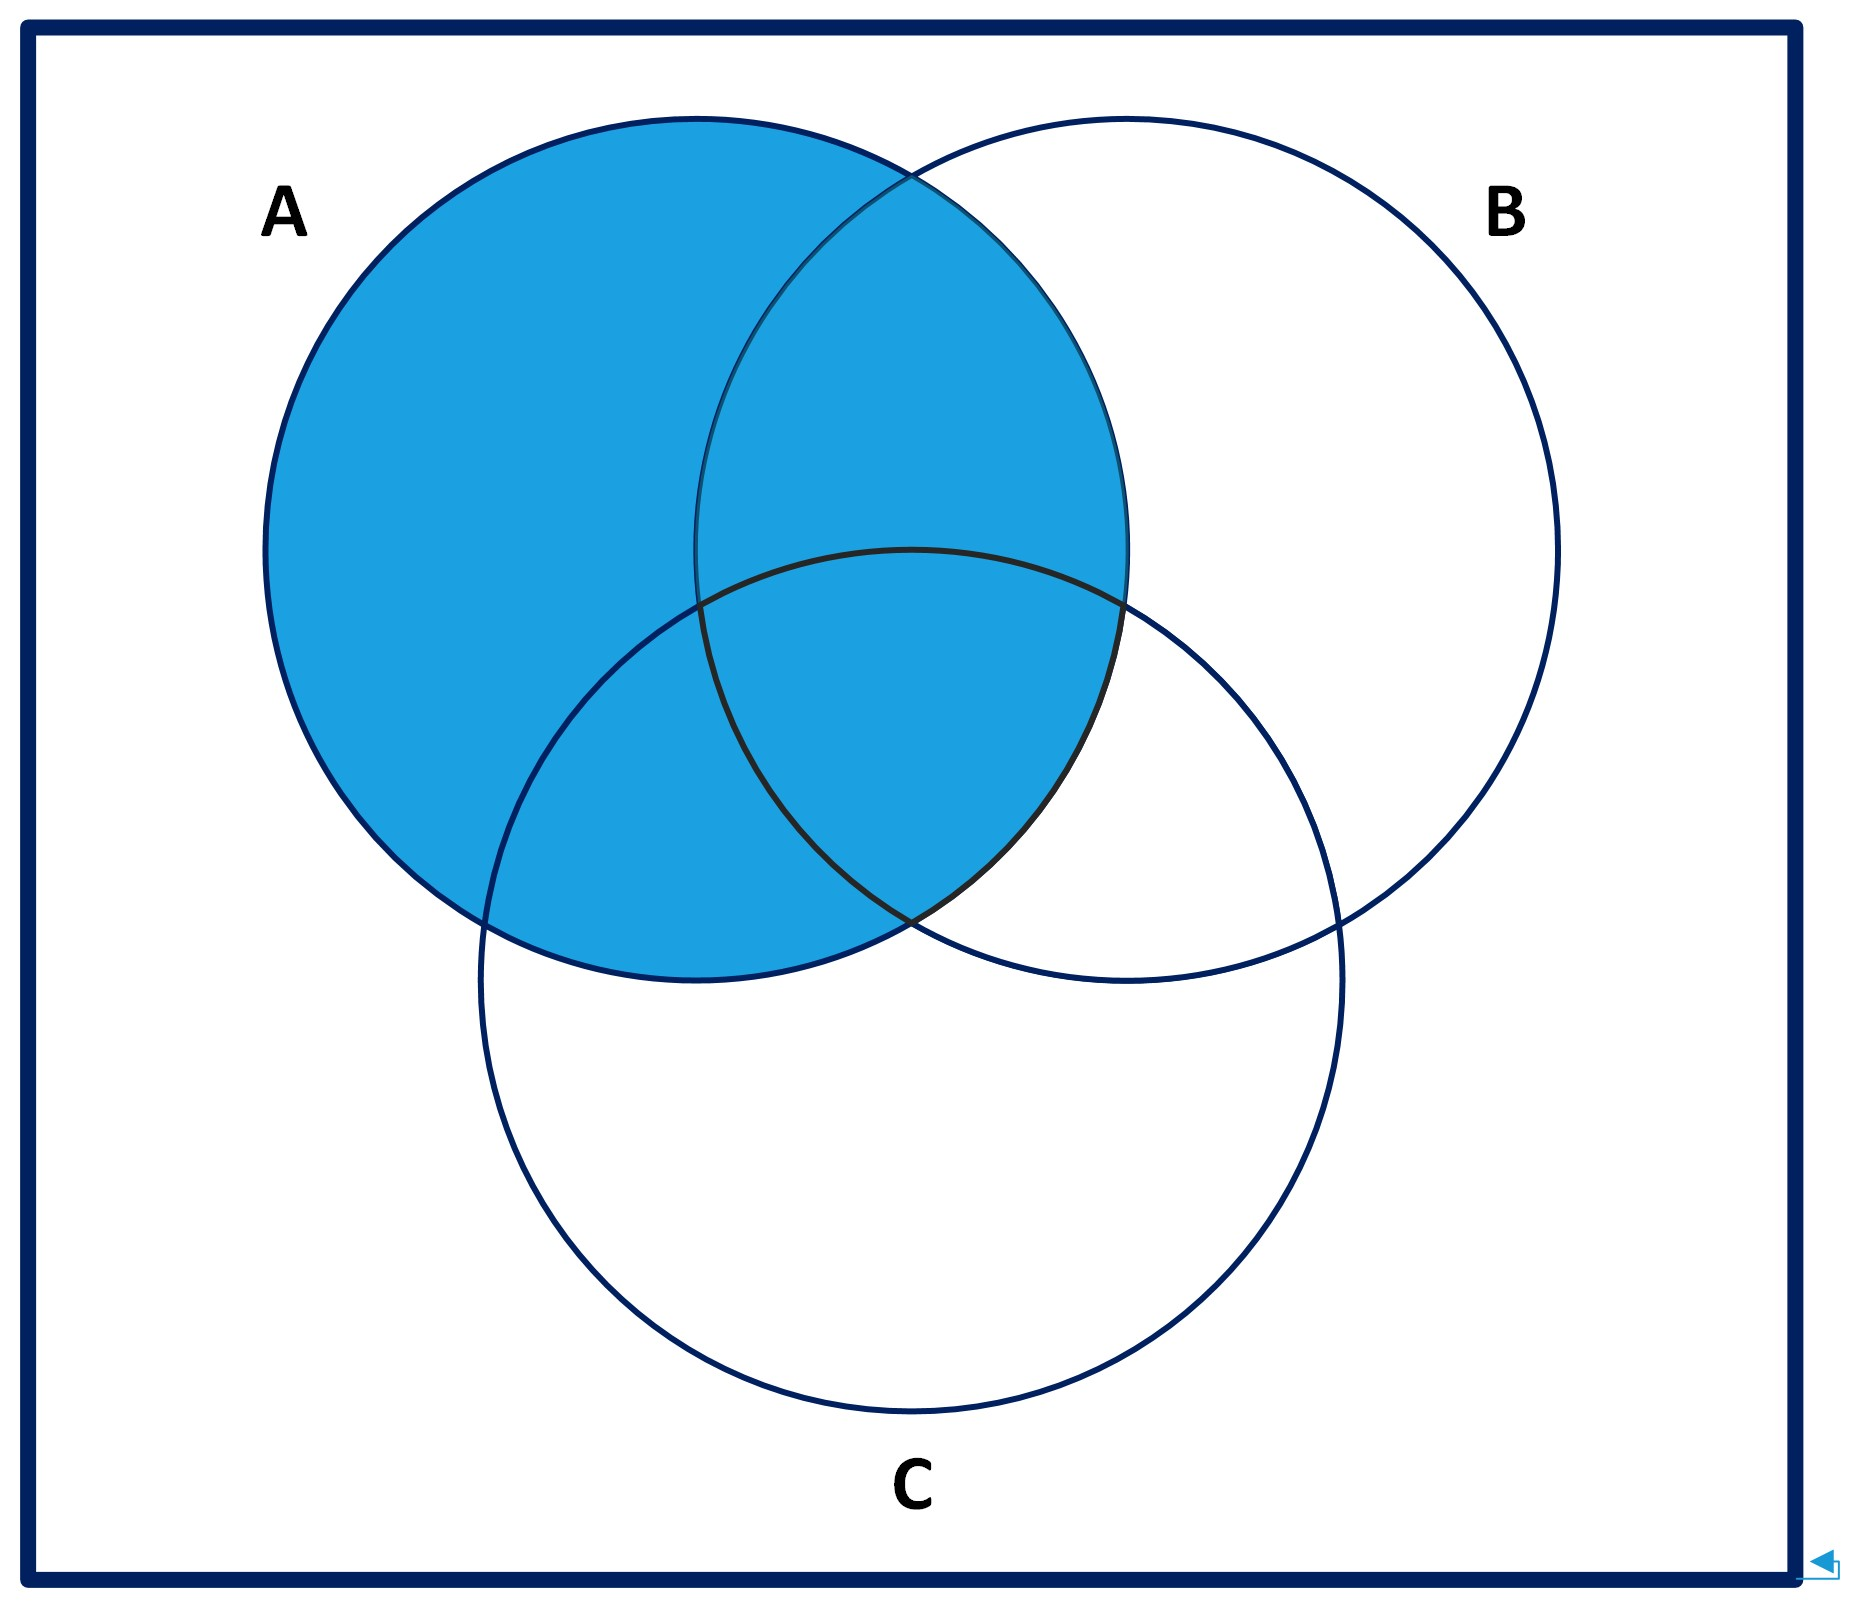
\includegraphics[width=\linewidth,height=1.5625in,keepaspectratio]{Images/venn1A.jpeg}
&
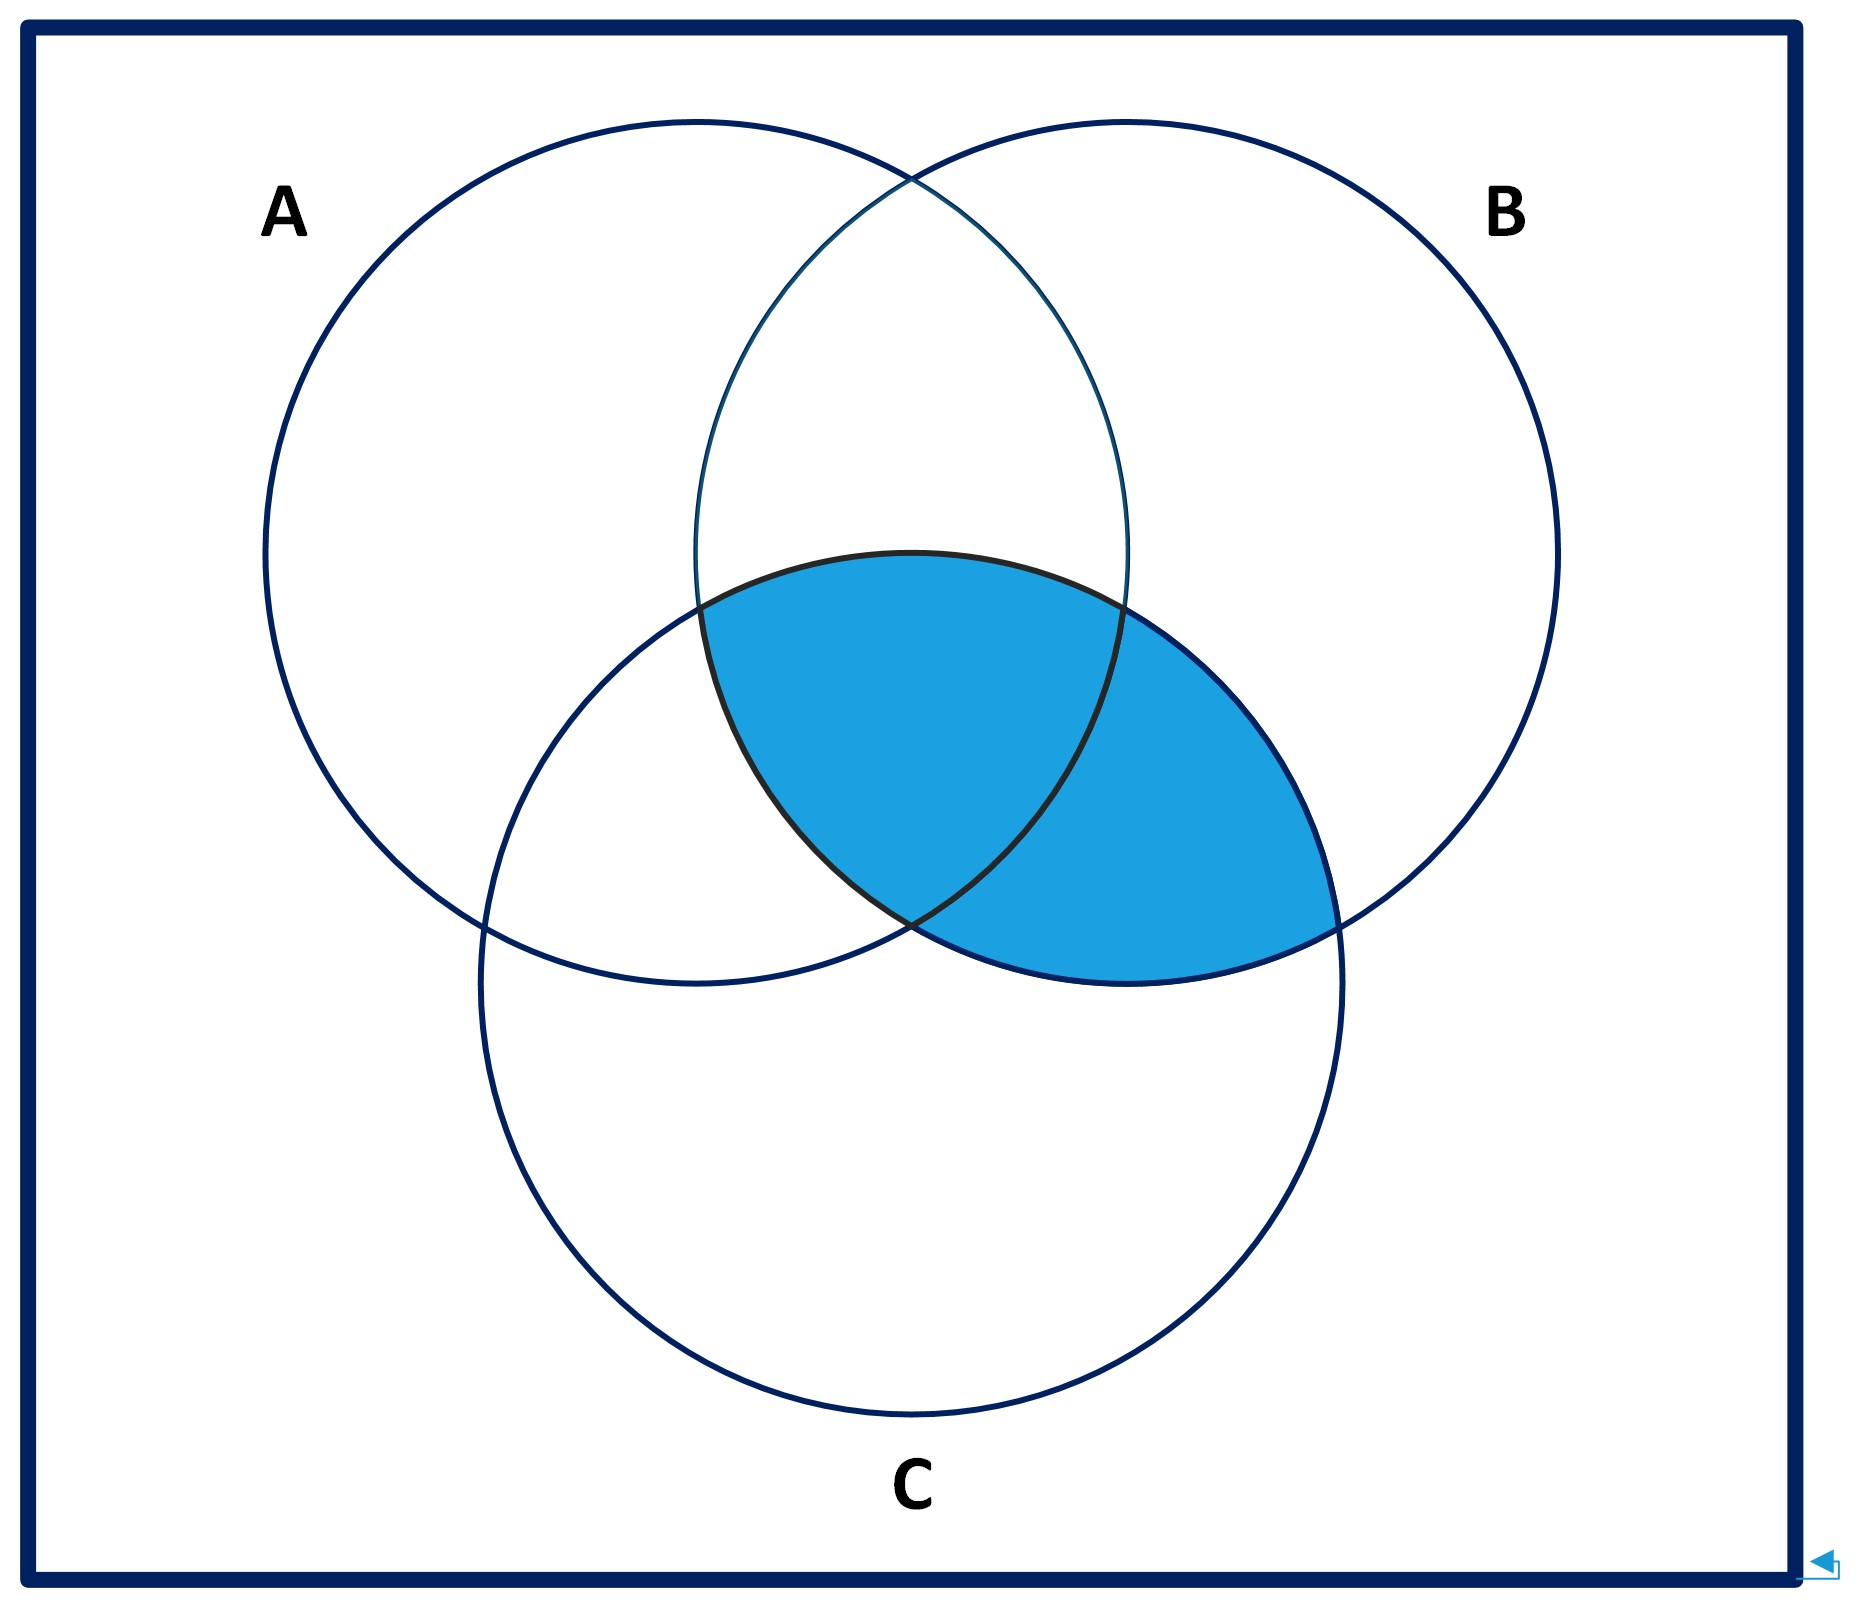
\includegraphics[width=\linewidth,height=1.5625in,keepaspectratio]{Images/venn1ByC.jpeg}
&
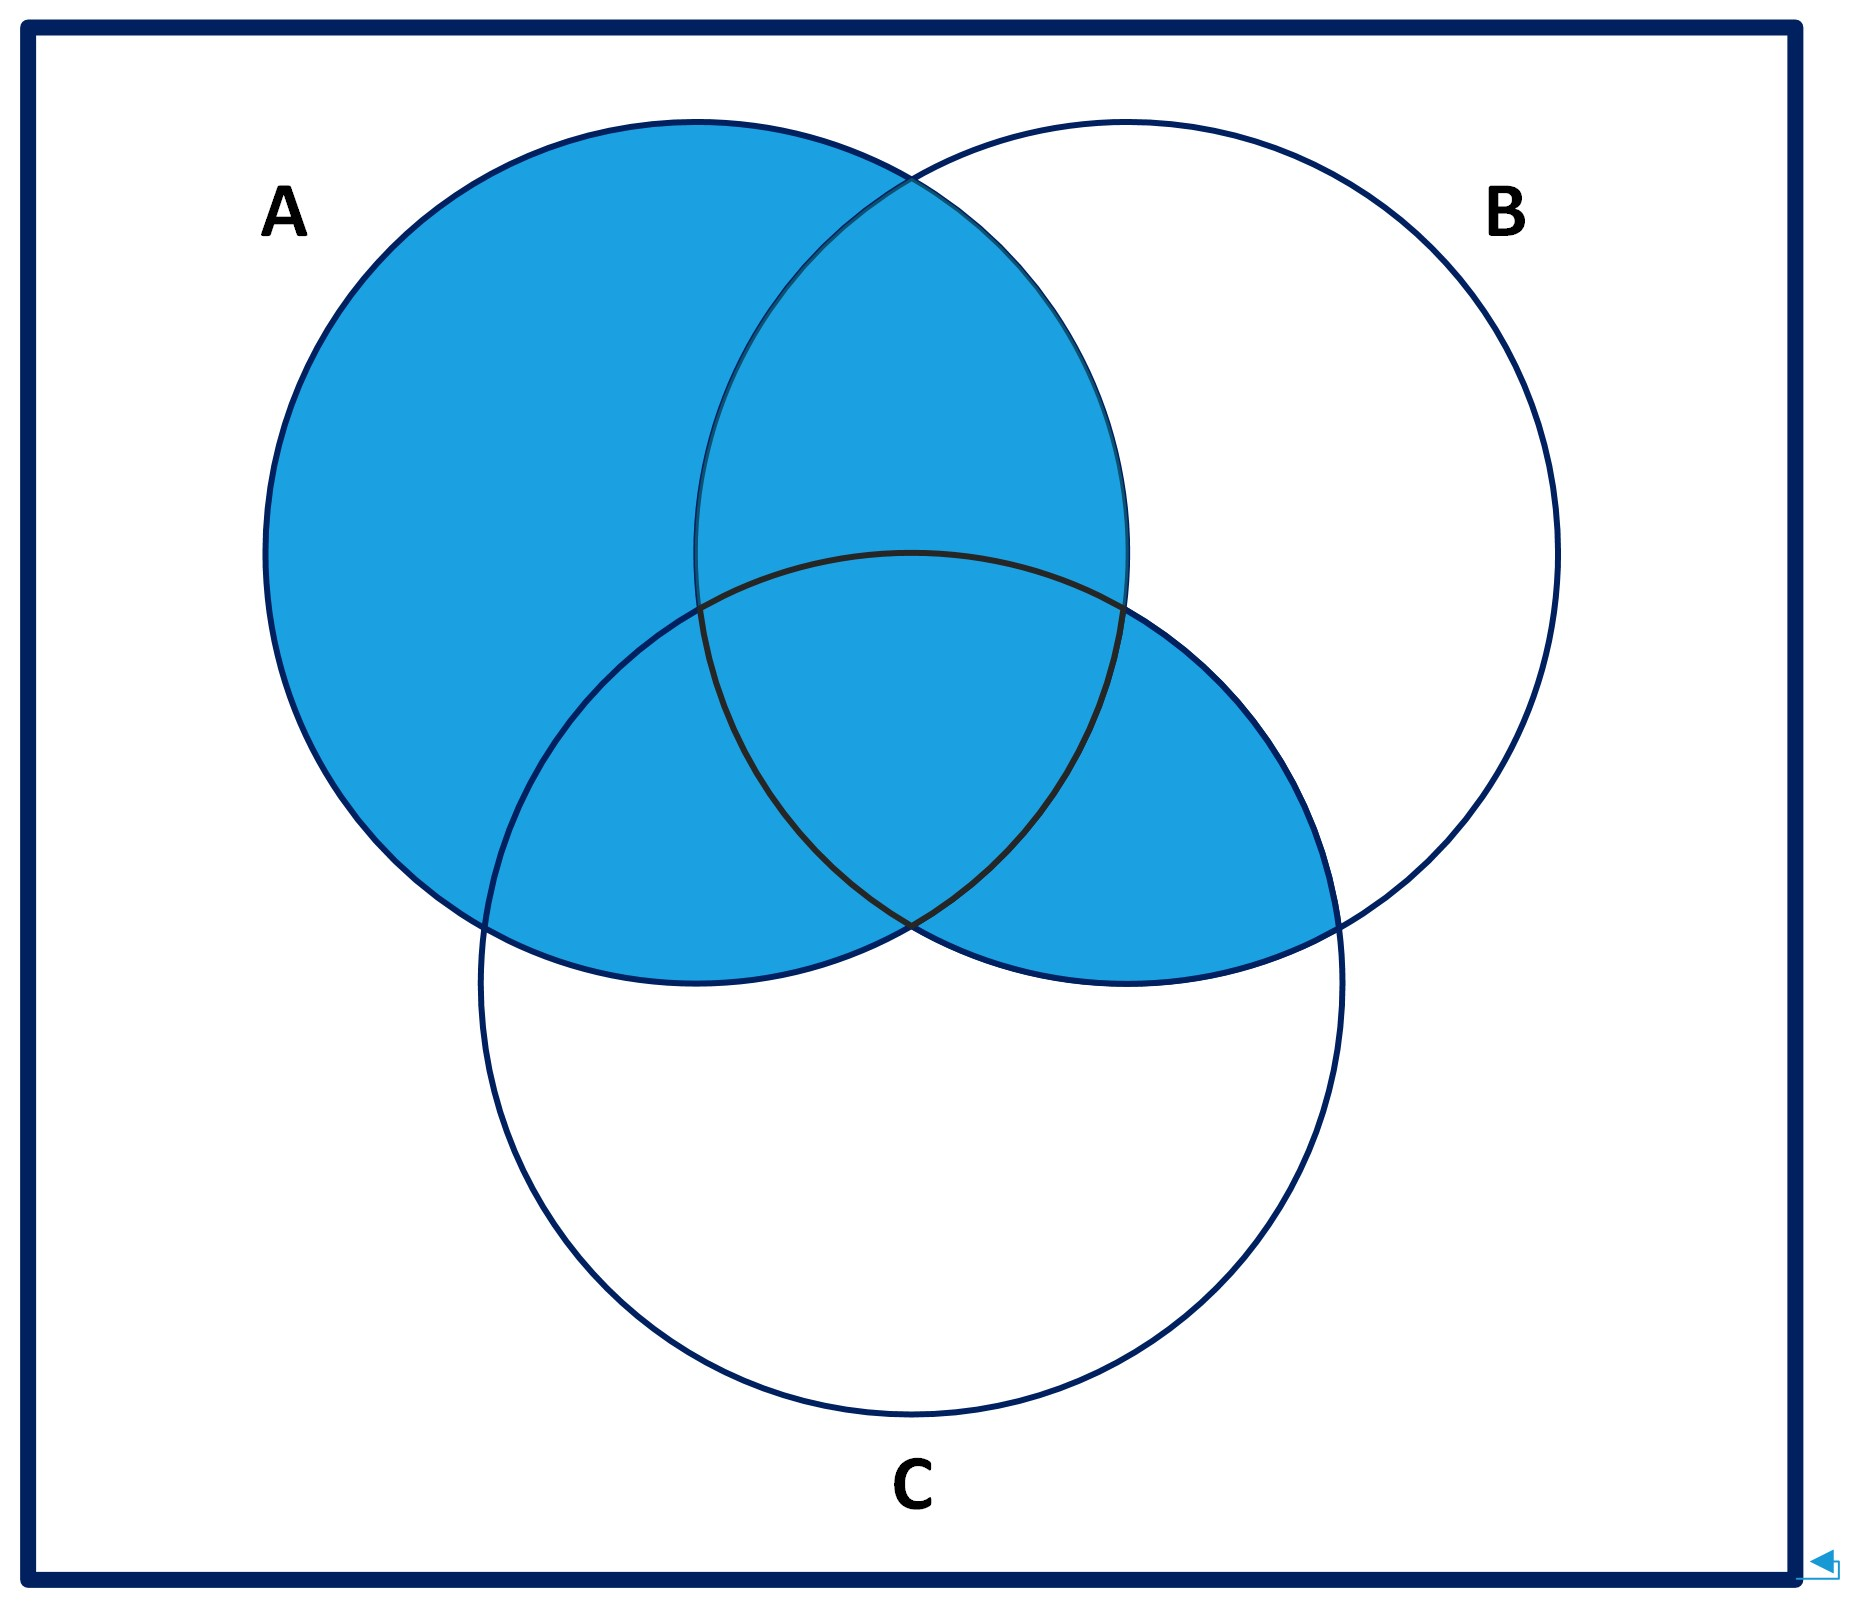
\includegraphics[width=\linewidth,height=1.5625in,keepaspectratio]{Images/venn1AUByC.jpeg} \\
\end{longtable}

\begin{longtable}[]{@{}
  >{\centering\arraybackslash}p{(\linewidth - 4\tabcolsep) * \real{0.3333}}
  >{\centering\arraybackslash}p{(\linewidth - 4\tabcolsep) * \real{0.3333}}
  >{\centering\arraybackslash}p{(\linewidth - 4\tabcolsep) * \real{0.3333}}@{}}
\toprule\noalign{}
\begin{minipage}[b]{\linewidth}\centering
\(A\cup B\)
\end{minipage} & \begin{minipage}[b]{\linewidth}\centering
\(A\cup C\)
\end{minipage} & \begin{minipage}[b]{\linewidth}\centering
\((A\cup B)\cap (A\cup C)\)
\end{minipage} \\
\midrule\noalign{}
\endhead
\bottomrule\noalign{}
\endlastfoot
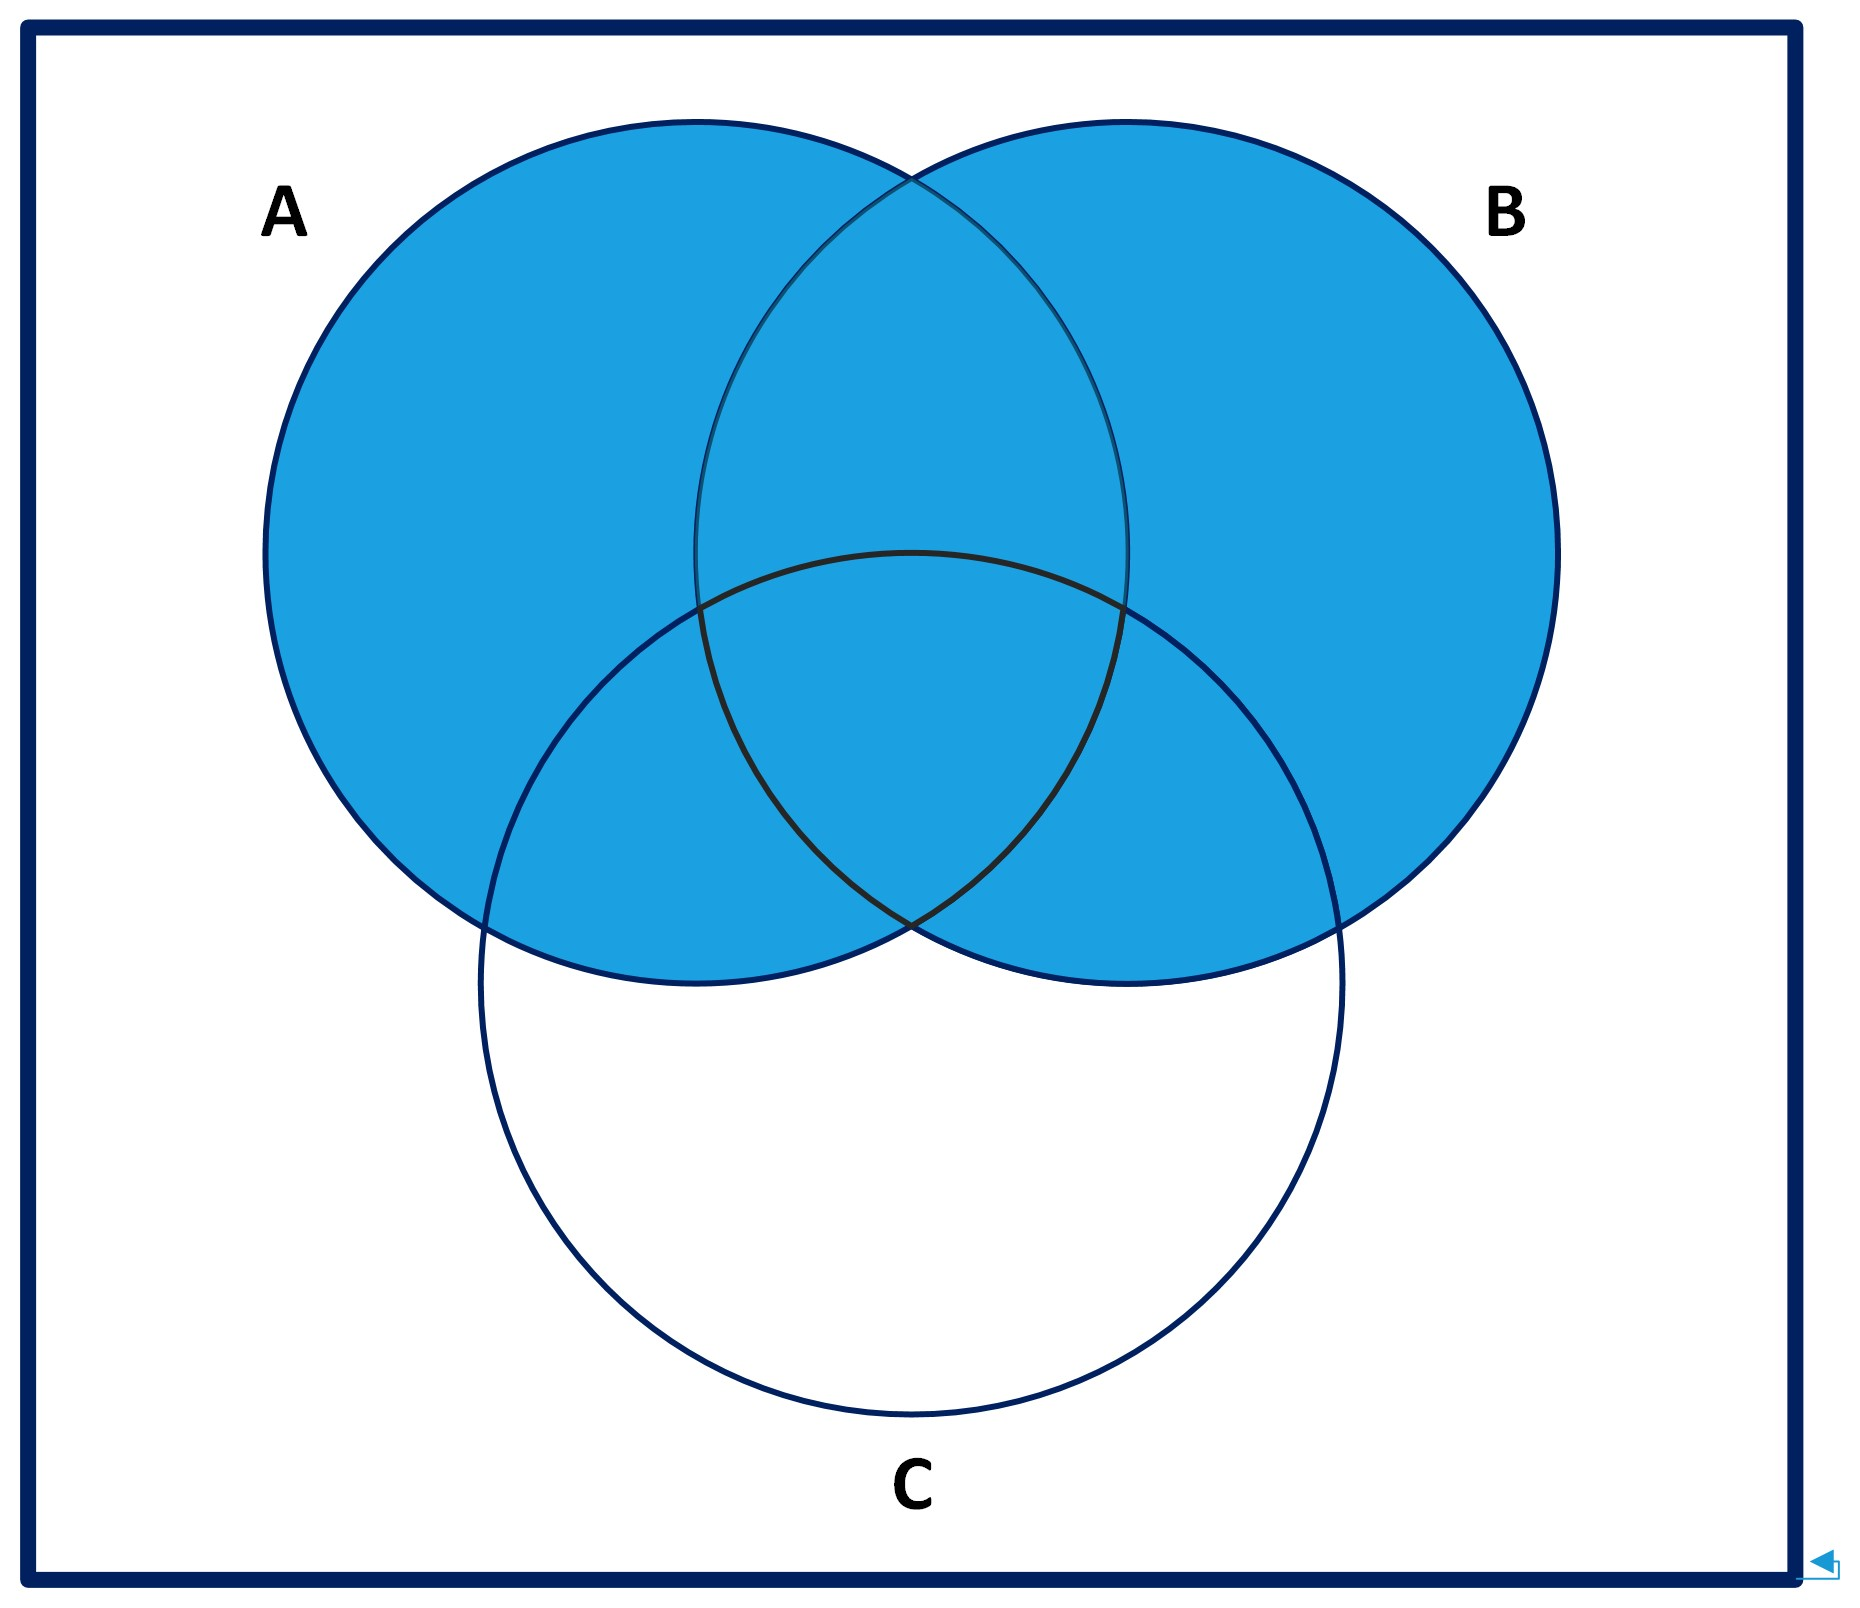
\includegraphics[width=\linewidth,height=1.5625in,keepaspectratio]{Images/venn1AoB.jpeg}
&
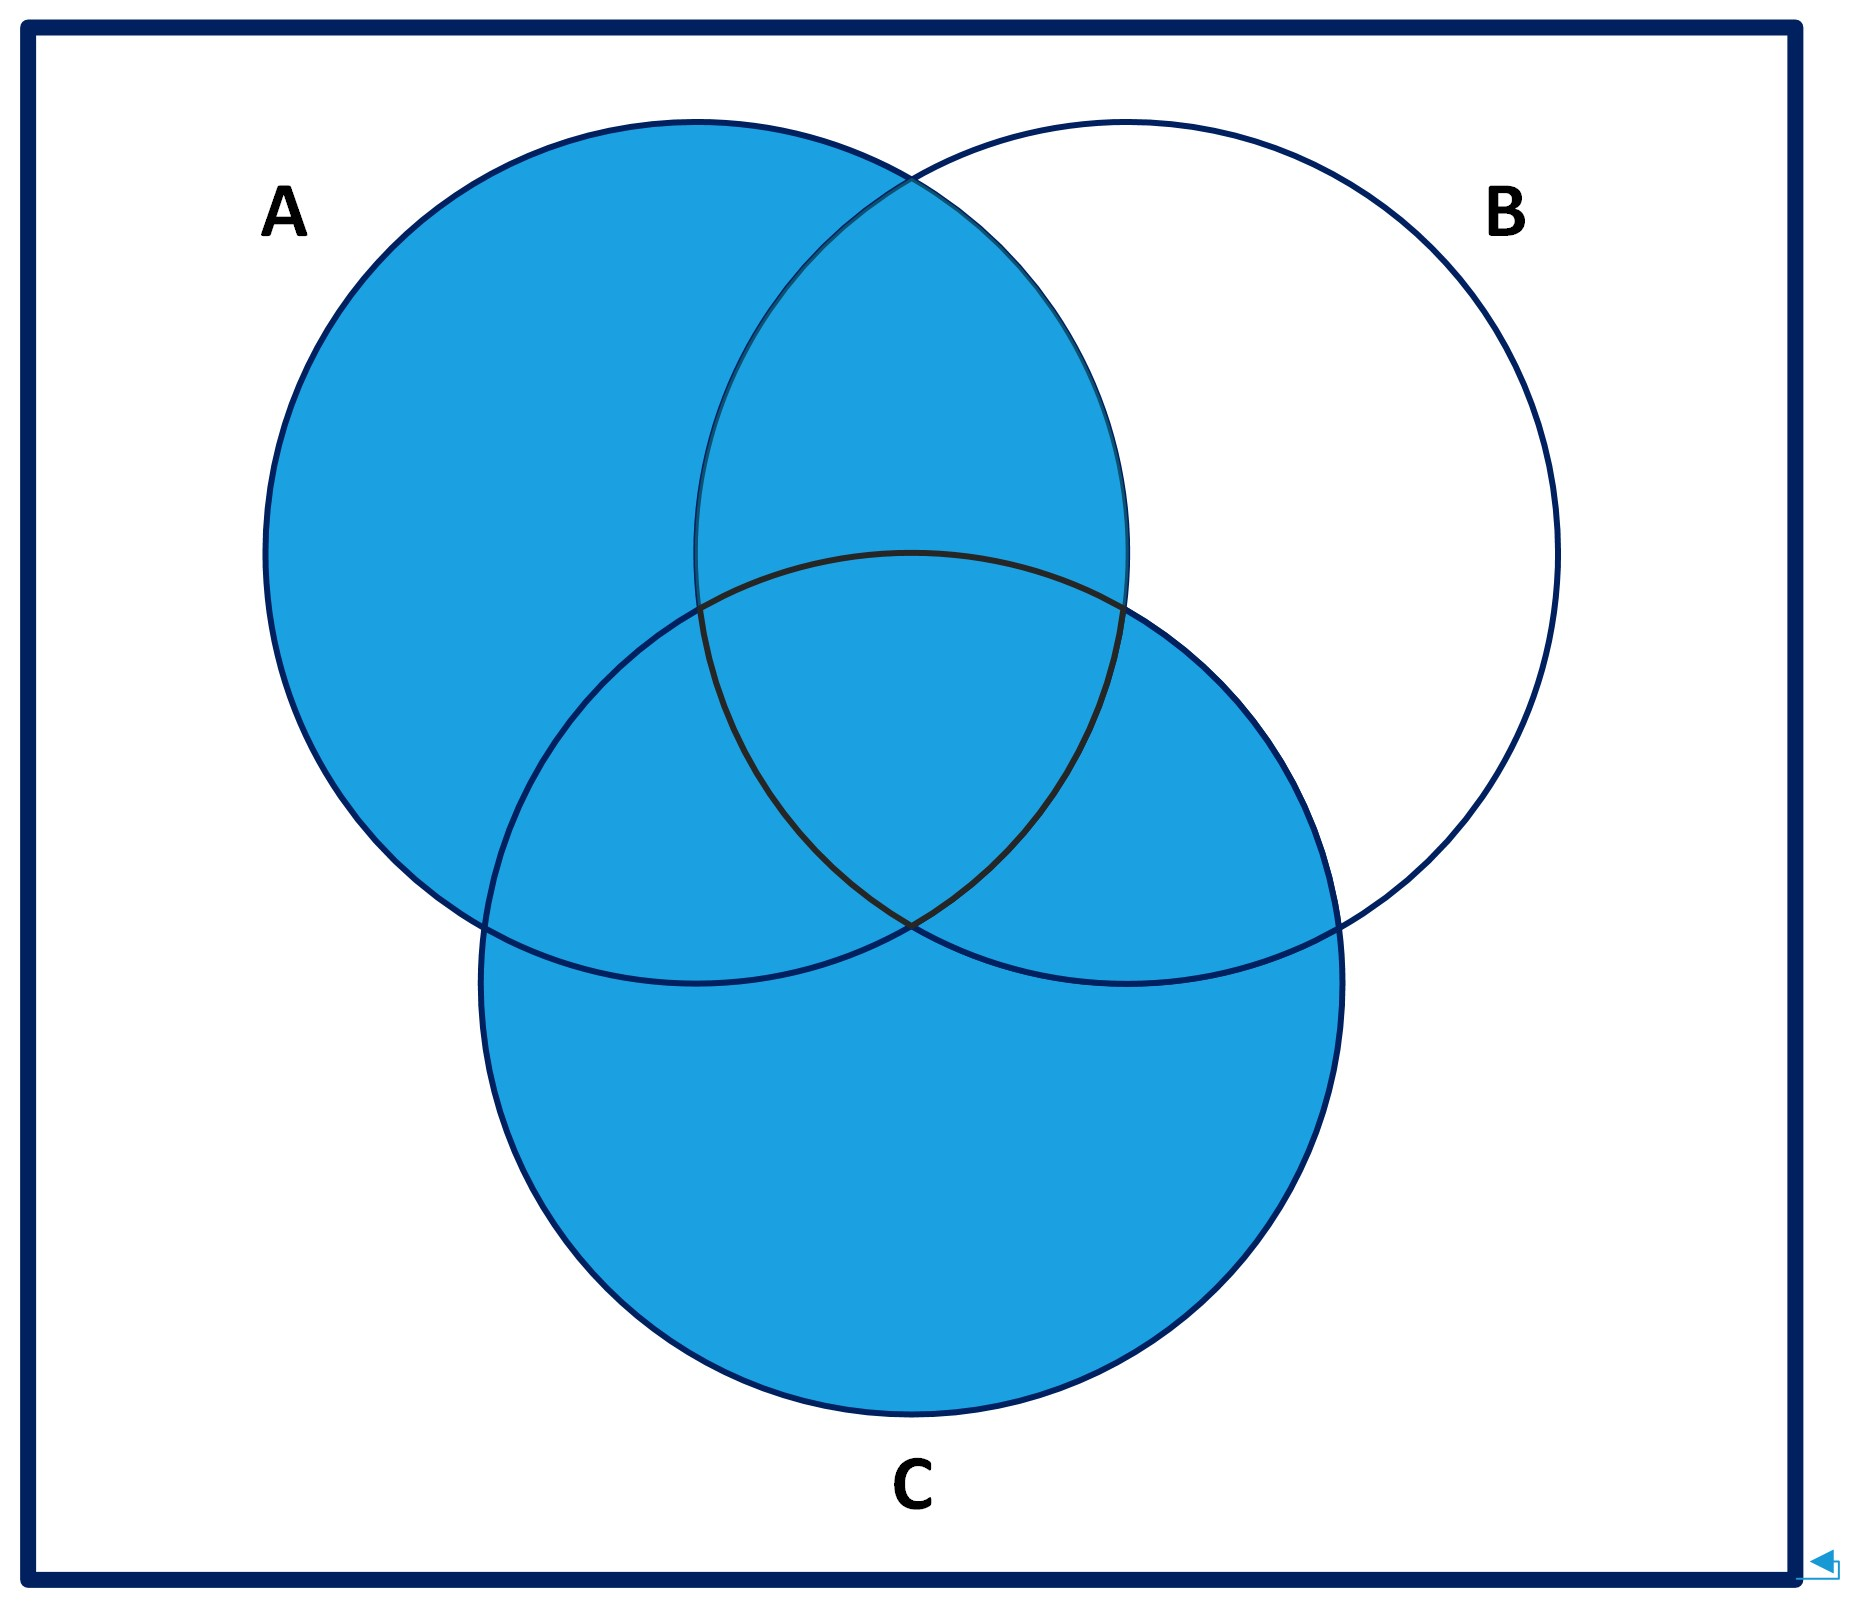
\includegraphics[width=\linewidth,height=1.5625in,keepaspectratio]{Images/venn1AoC.jpeg}
&
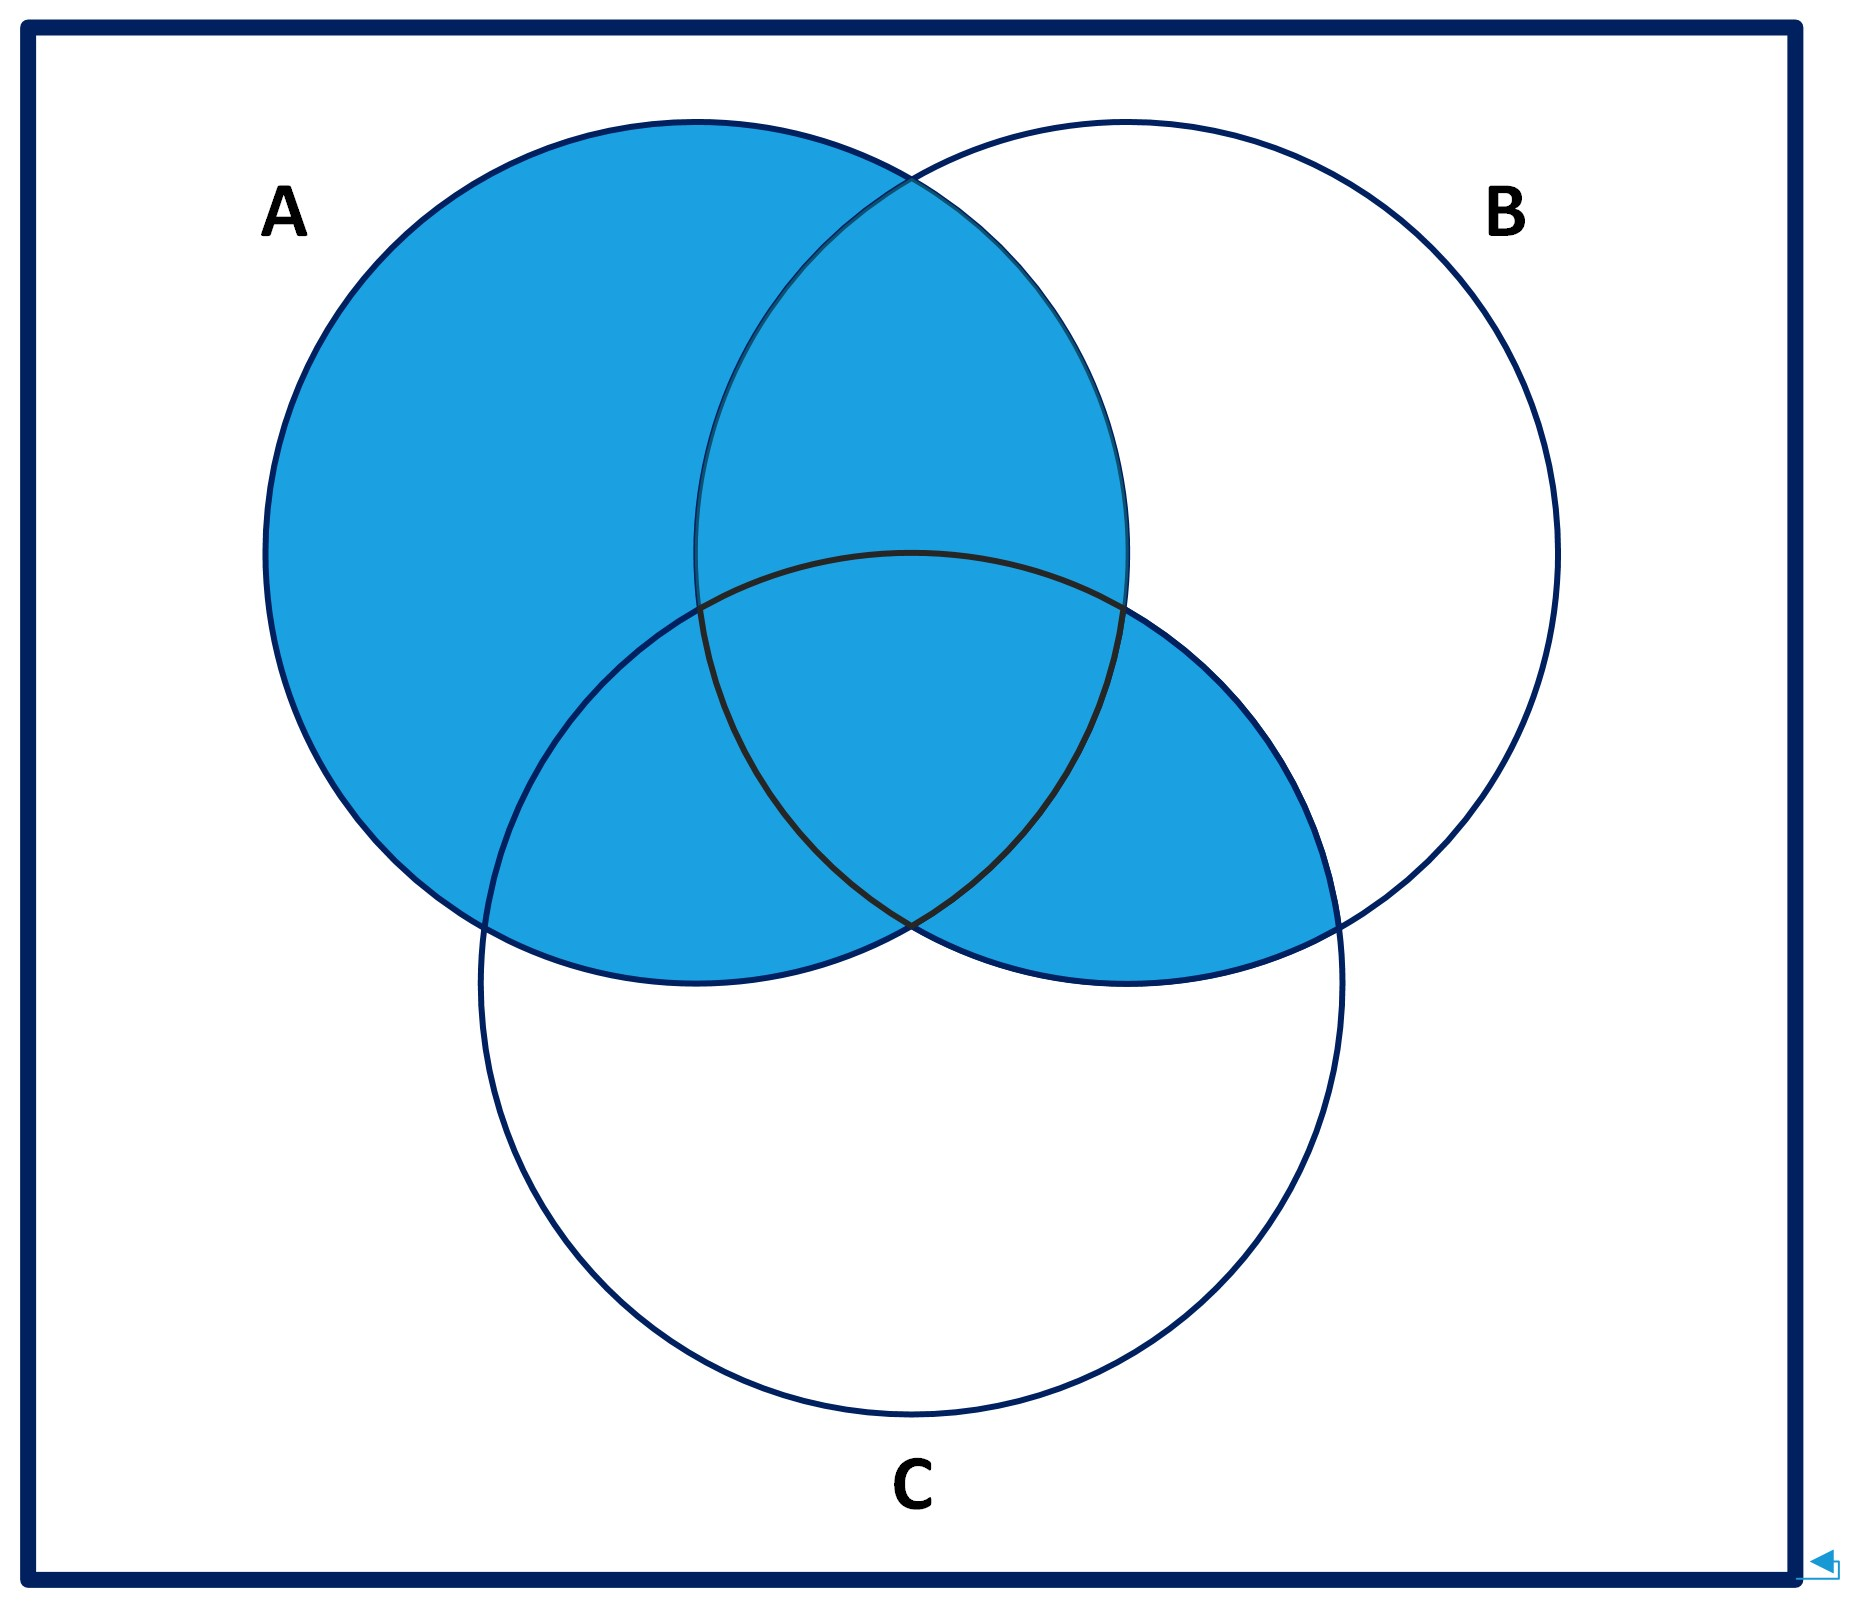
\includegraphics[width=\linewidth,height=1.5625in,keepaspectratio]{Images/venn1AUByC.jpeg} \\
\end{longtable}

Complementario del complementario

\[(A^c)^c=A\]

\begin{longtable}[]{@{}
  >{\centering\arraybackslash}p{(\linewidth - 4\tabcolsep) * \real{0.3333}}
  >{\centering\arraybackslash}p{(\linewidth - 4\tabcolsep) * \real{0.3333}}
  >{\centering\arraybackslash}p{(\linewidth - 4\tabcolsep) * \real{0.3333}}@{}}
\toprule\noalign{}
\begin{minipage}[b]{\linewidth}\centering
\(A\)
\end{minipage} & \begin{minipage}[b]{\linewidth}\centering
\(A^c\)
\end{minipage} & \begin{minipage}[b]{\linewidth}\centering
\((A^c)^c\)
\end{minipage} \\
\midrule\noalign{}
\endhead
\bottomrule\noalign{}
\endlastfoot
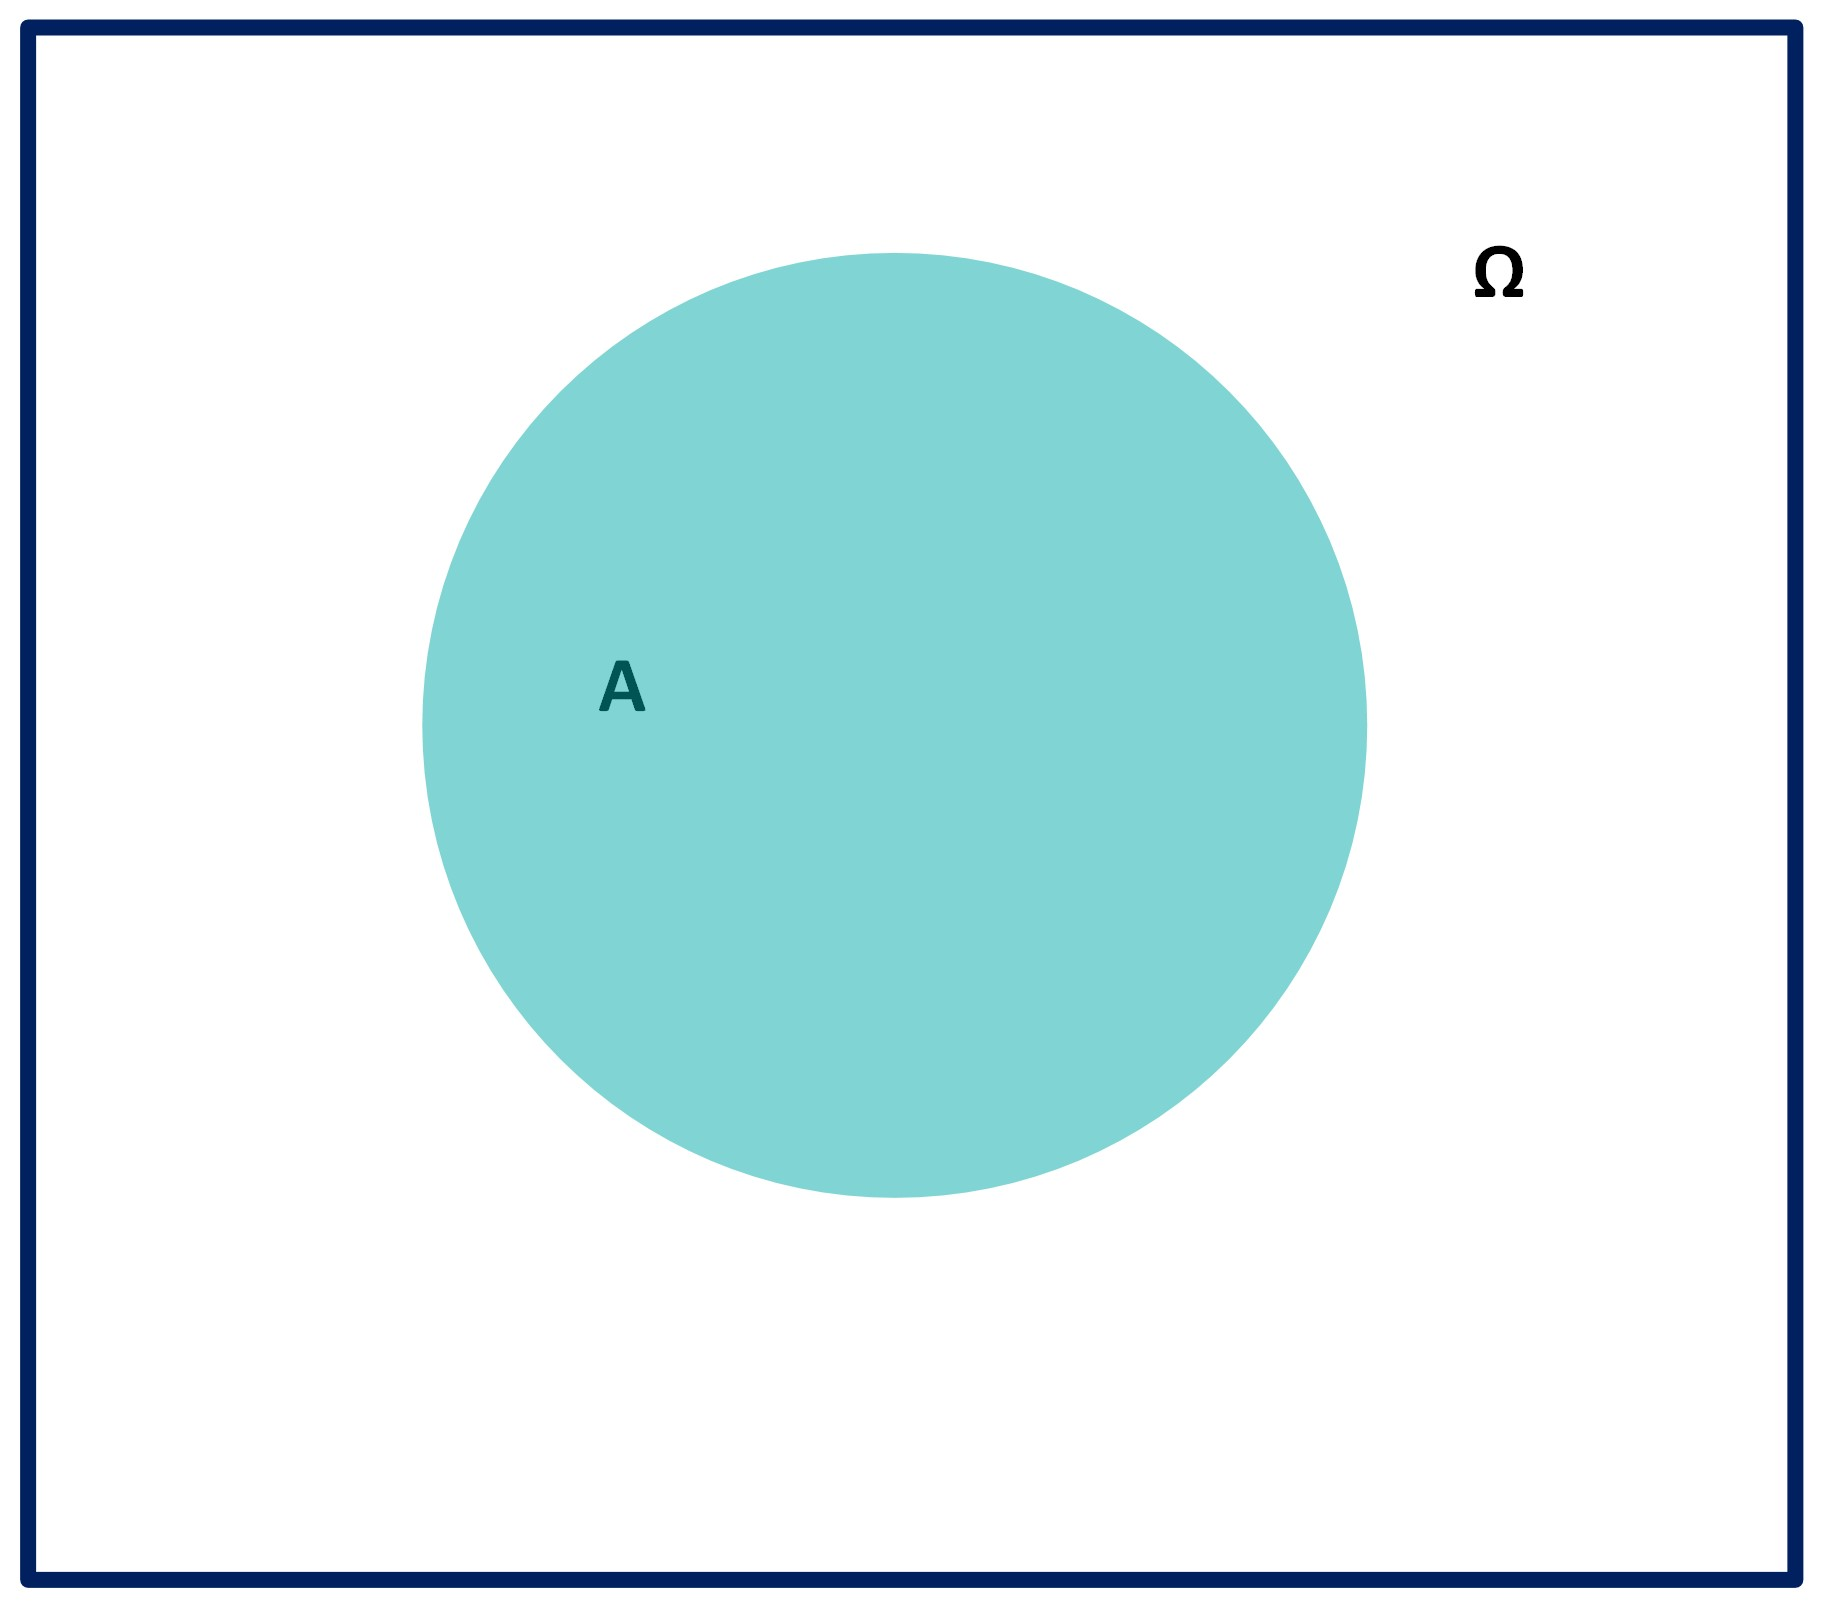
\includegraphics[width=\linewidth,height=1.5625in,keepaspectratio]{Images/venn1A_solo.jpeg}
&
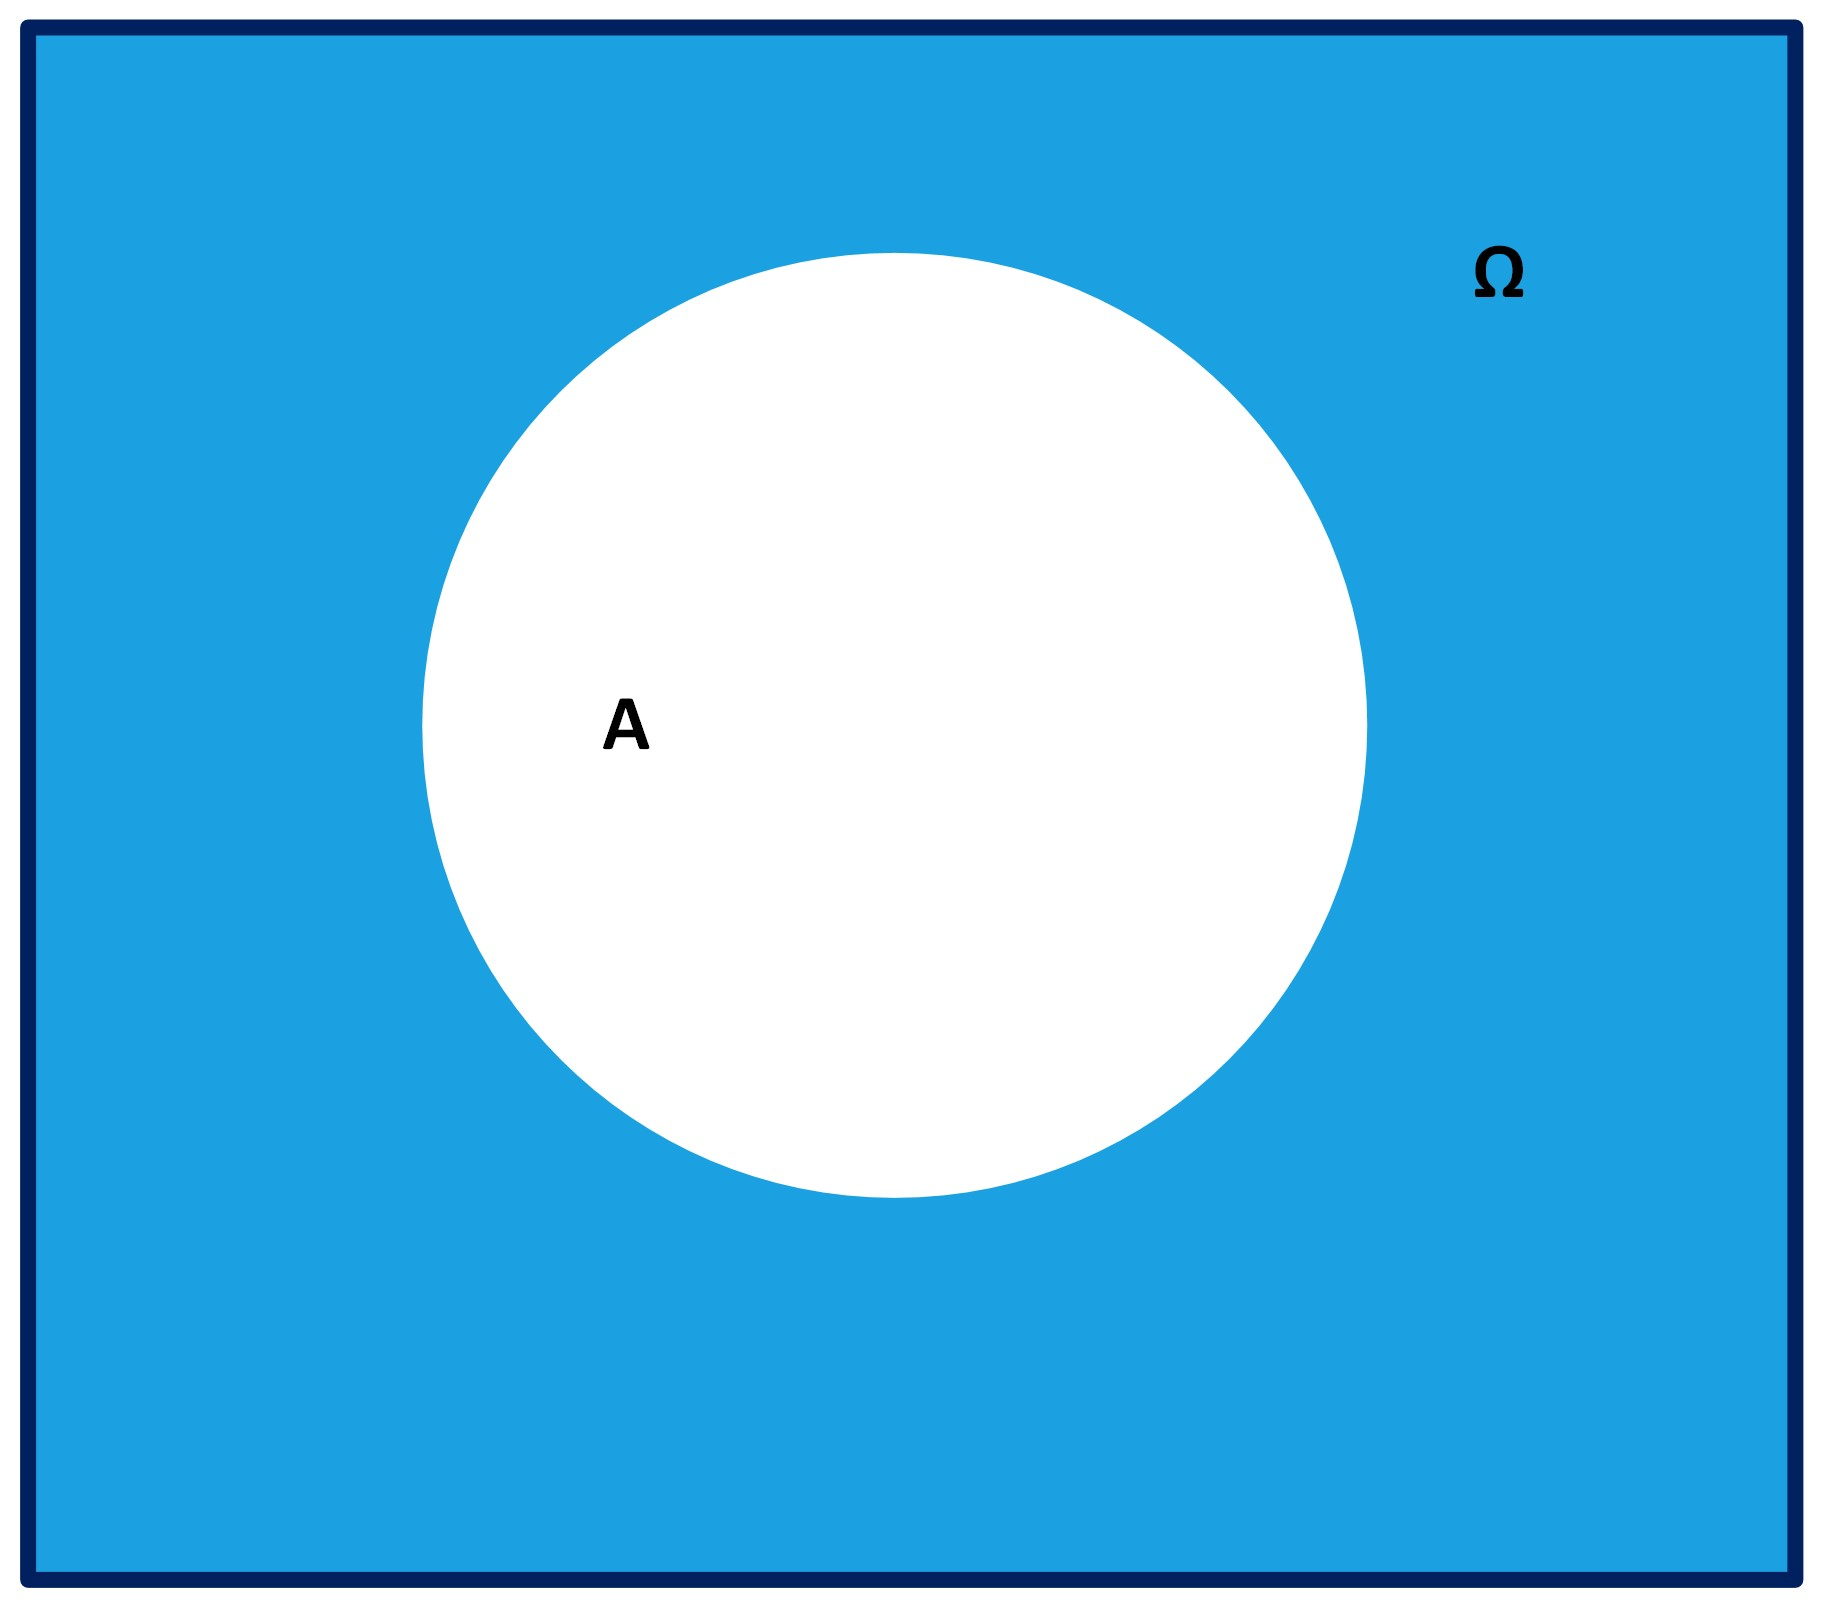
\includegraphics[width=\linewidth,height=1.5625in,keepaspectratio]{Images/venn1solo_Ac.jpeg}
&
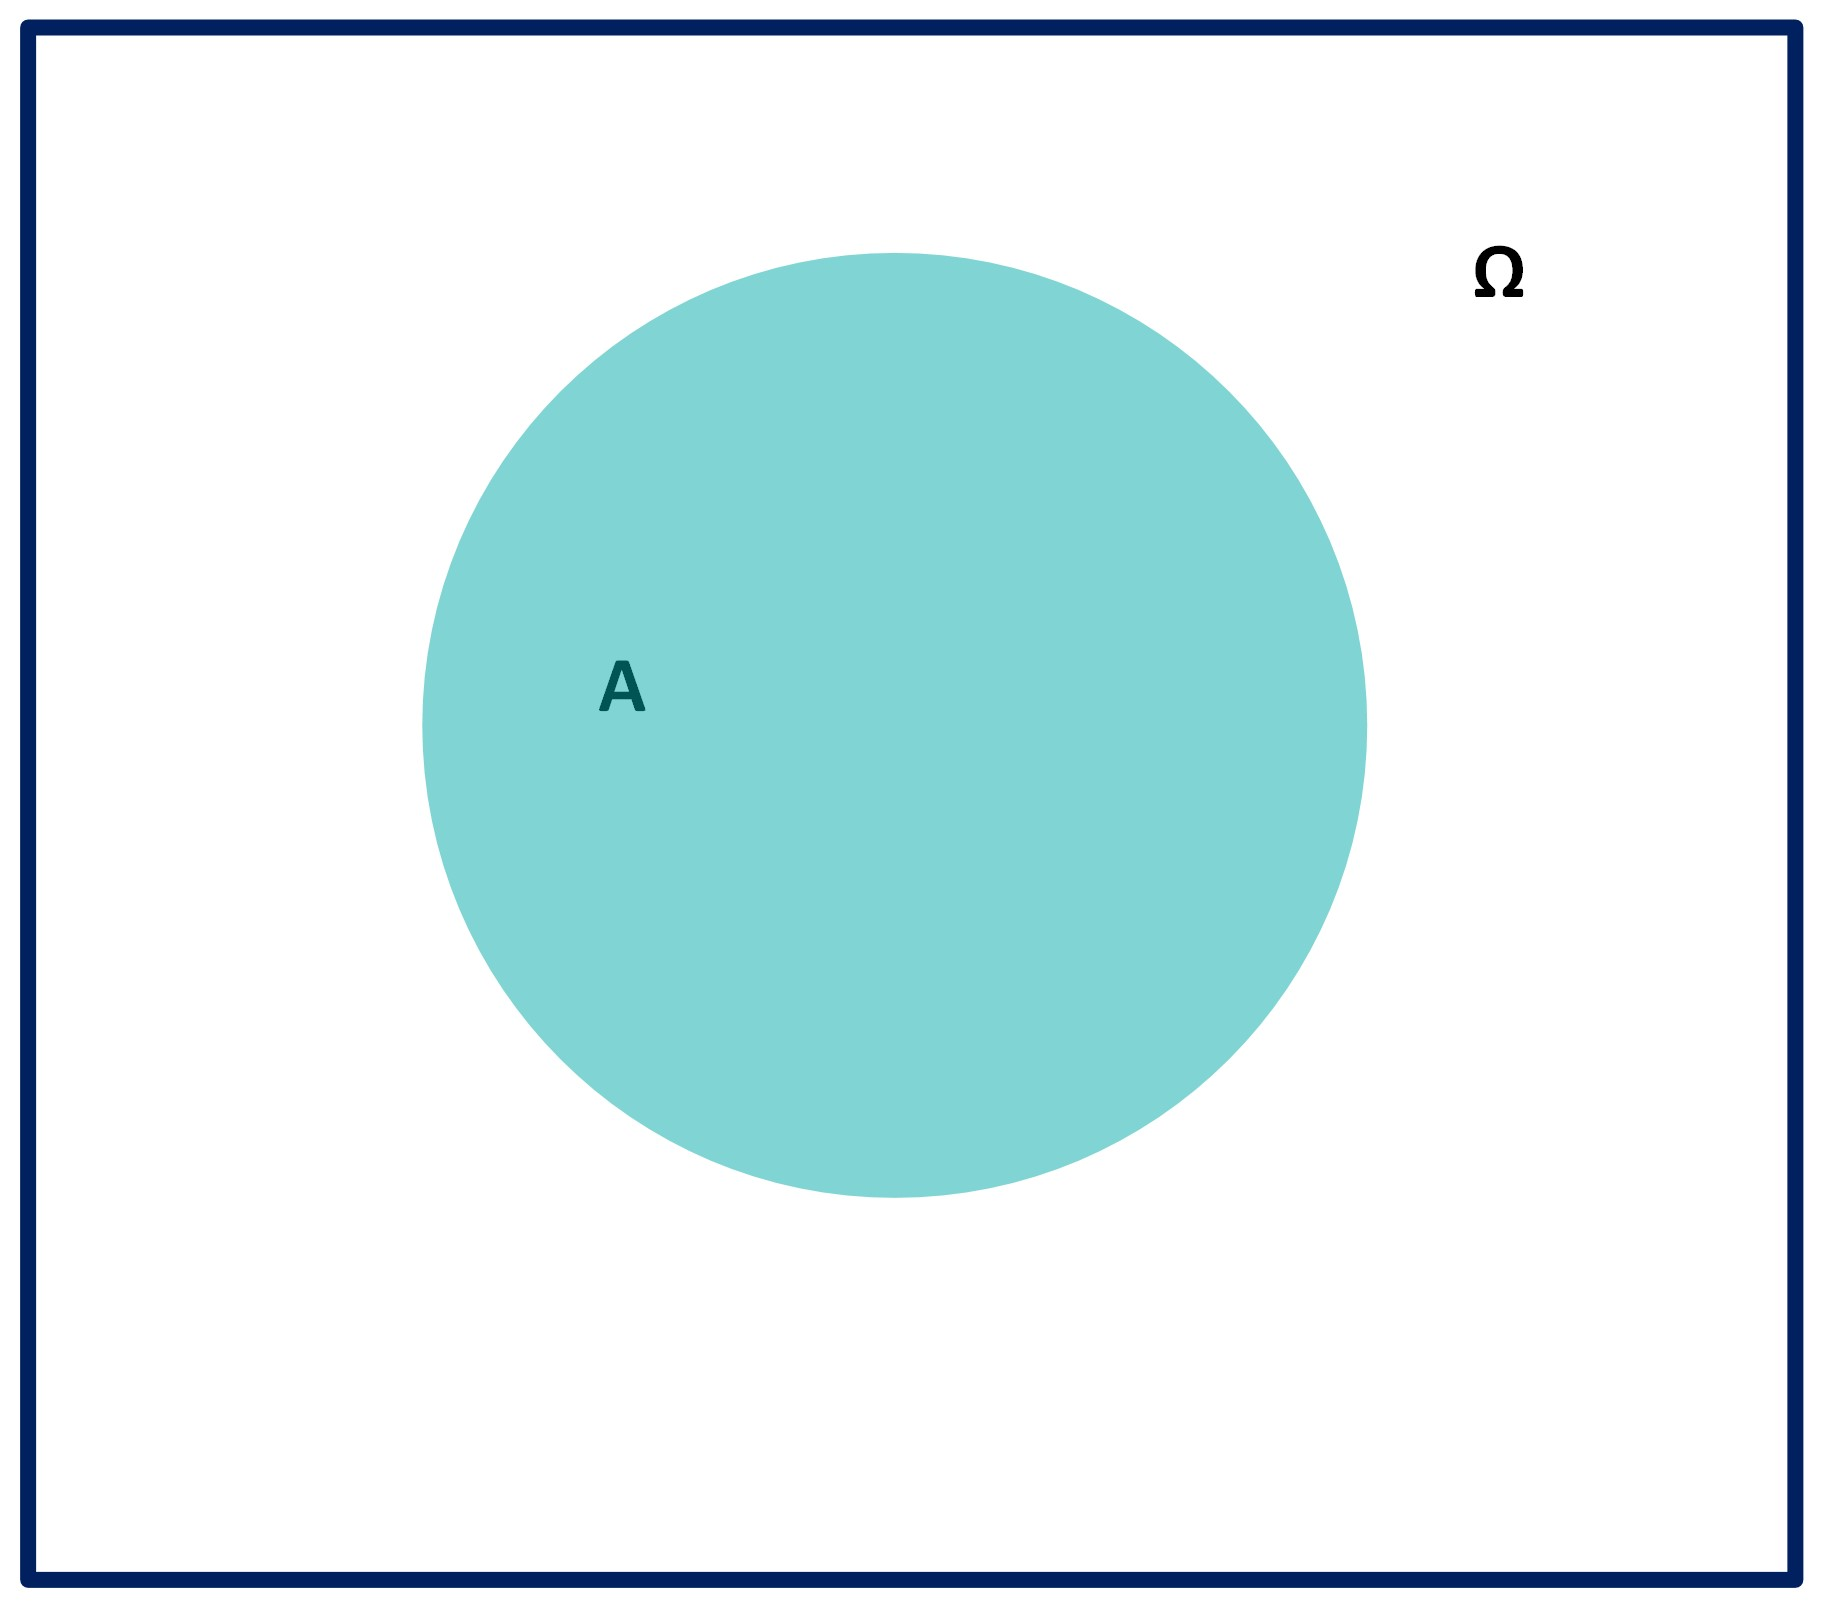
\includegraphics[width=\linewidth,height=1.5625in,keepaspectratio]{Images/venn1A_solo.jpeg} \\
\end{longtable}

Leyes de De Morgan

\[(A\cup B)^c=A^c\cap B^c\]

\begin{longtable}[]{@{}
  >{\centering\arraybackslash}p{(\linewidth - 2\tabcolsep) * \real{0.5000}}
  >{\centering\arraybackslash}p{(\linewidth - 2\tabcolsep) * \real{0.5000}}@{}}
\toprule\noalign{}
\begin{minipage}[b]{\linewidth}\centering
\(A\cup B\)
\end{minipage} & \begin{minipage}[b]{\linewidth}\centering
\((A\cup B)^c\)
\end{minipage} \\
\midrule\noalign{}
\endhead
\bottomrule\noalign{}
\endlastfoot
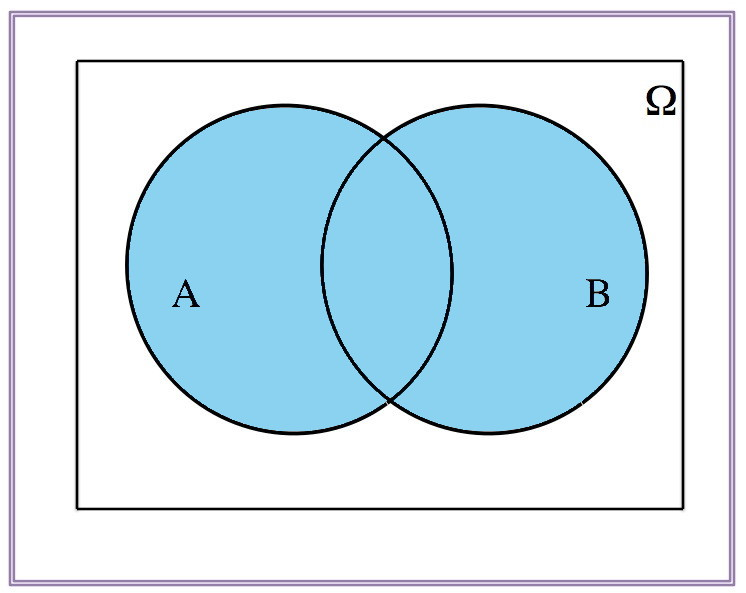
\includegraphics[width=\linewidth,height=1.5625in,keepaspectratio]{Images/proba1dibujos/demorgan6.jpg}
&
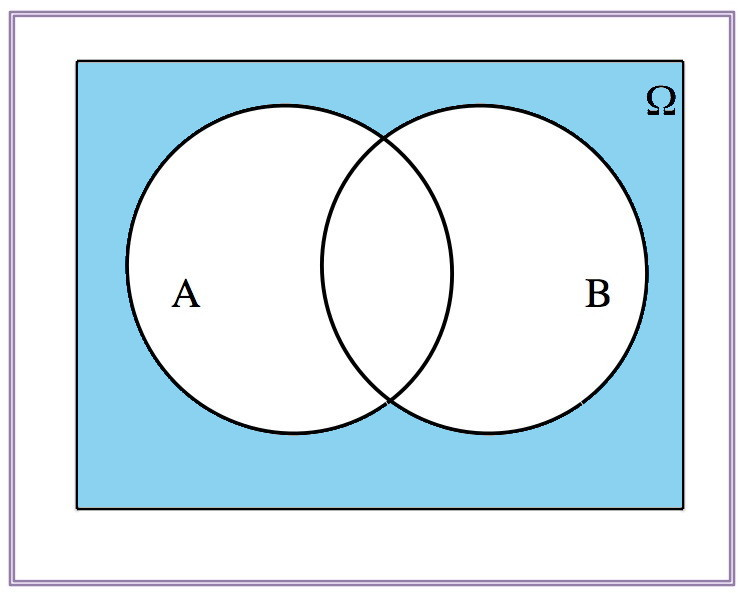
\includegraphics[width=\linewidth,height=1.5625in,keepaspectratio]{Images/proba1dibujos/demorgan7.jpg} \\
\end{longtable}

\[(A\cup B)^c=A^c\cap B^c\]

\begin{longtable}[]{@{}
  >{\centering\arraybackslash}p{(\linewidth - 4\tabcolsep) * \real{0.3333}}
  >{\centering\arraybackslash}p{(\linewidth - 4\tabcolsep) * \real{0.3333}}
  >{\centering\arraybackslash}p{(\linewidth - 4\tabcolsep) * \real{0.3333}}@{}}
\toprule\noalign{}
\begin{minipage}[b]{\linewidth}\centering
\(A^c\)
\end{minipage} & \begin{minipage}[b]{\linewidth}\centering
\(B^c\)
\end{minipage} & \begin{minipage}[b]{\linewidth}\centering
\(A^c\cap B^c\)
\end{minipage} \\
\midrule\noalign{}
\endhead
\bottomrule\noalign{}
\endlastfoot
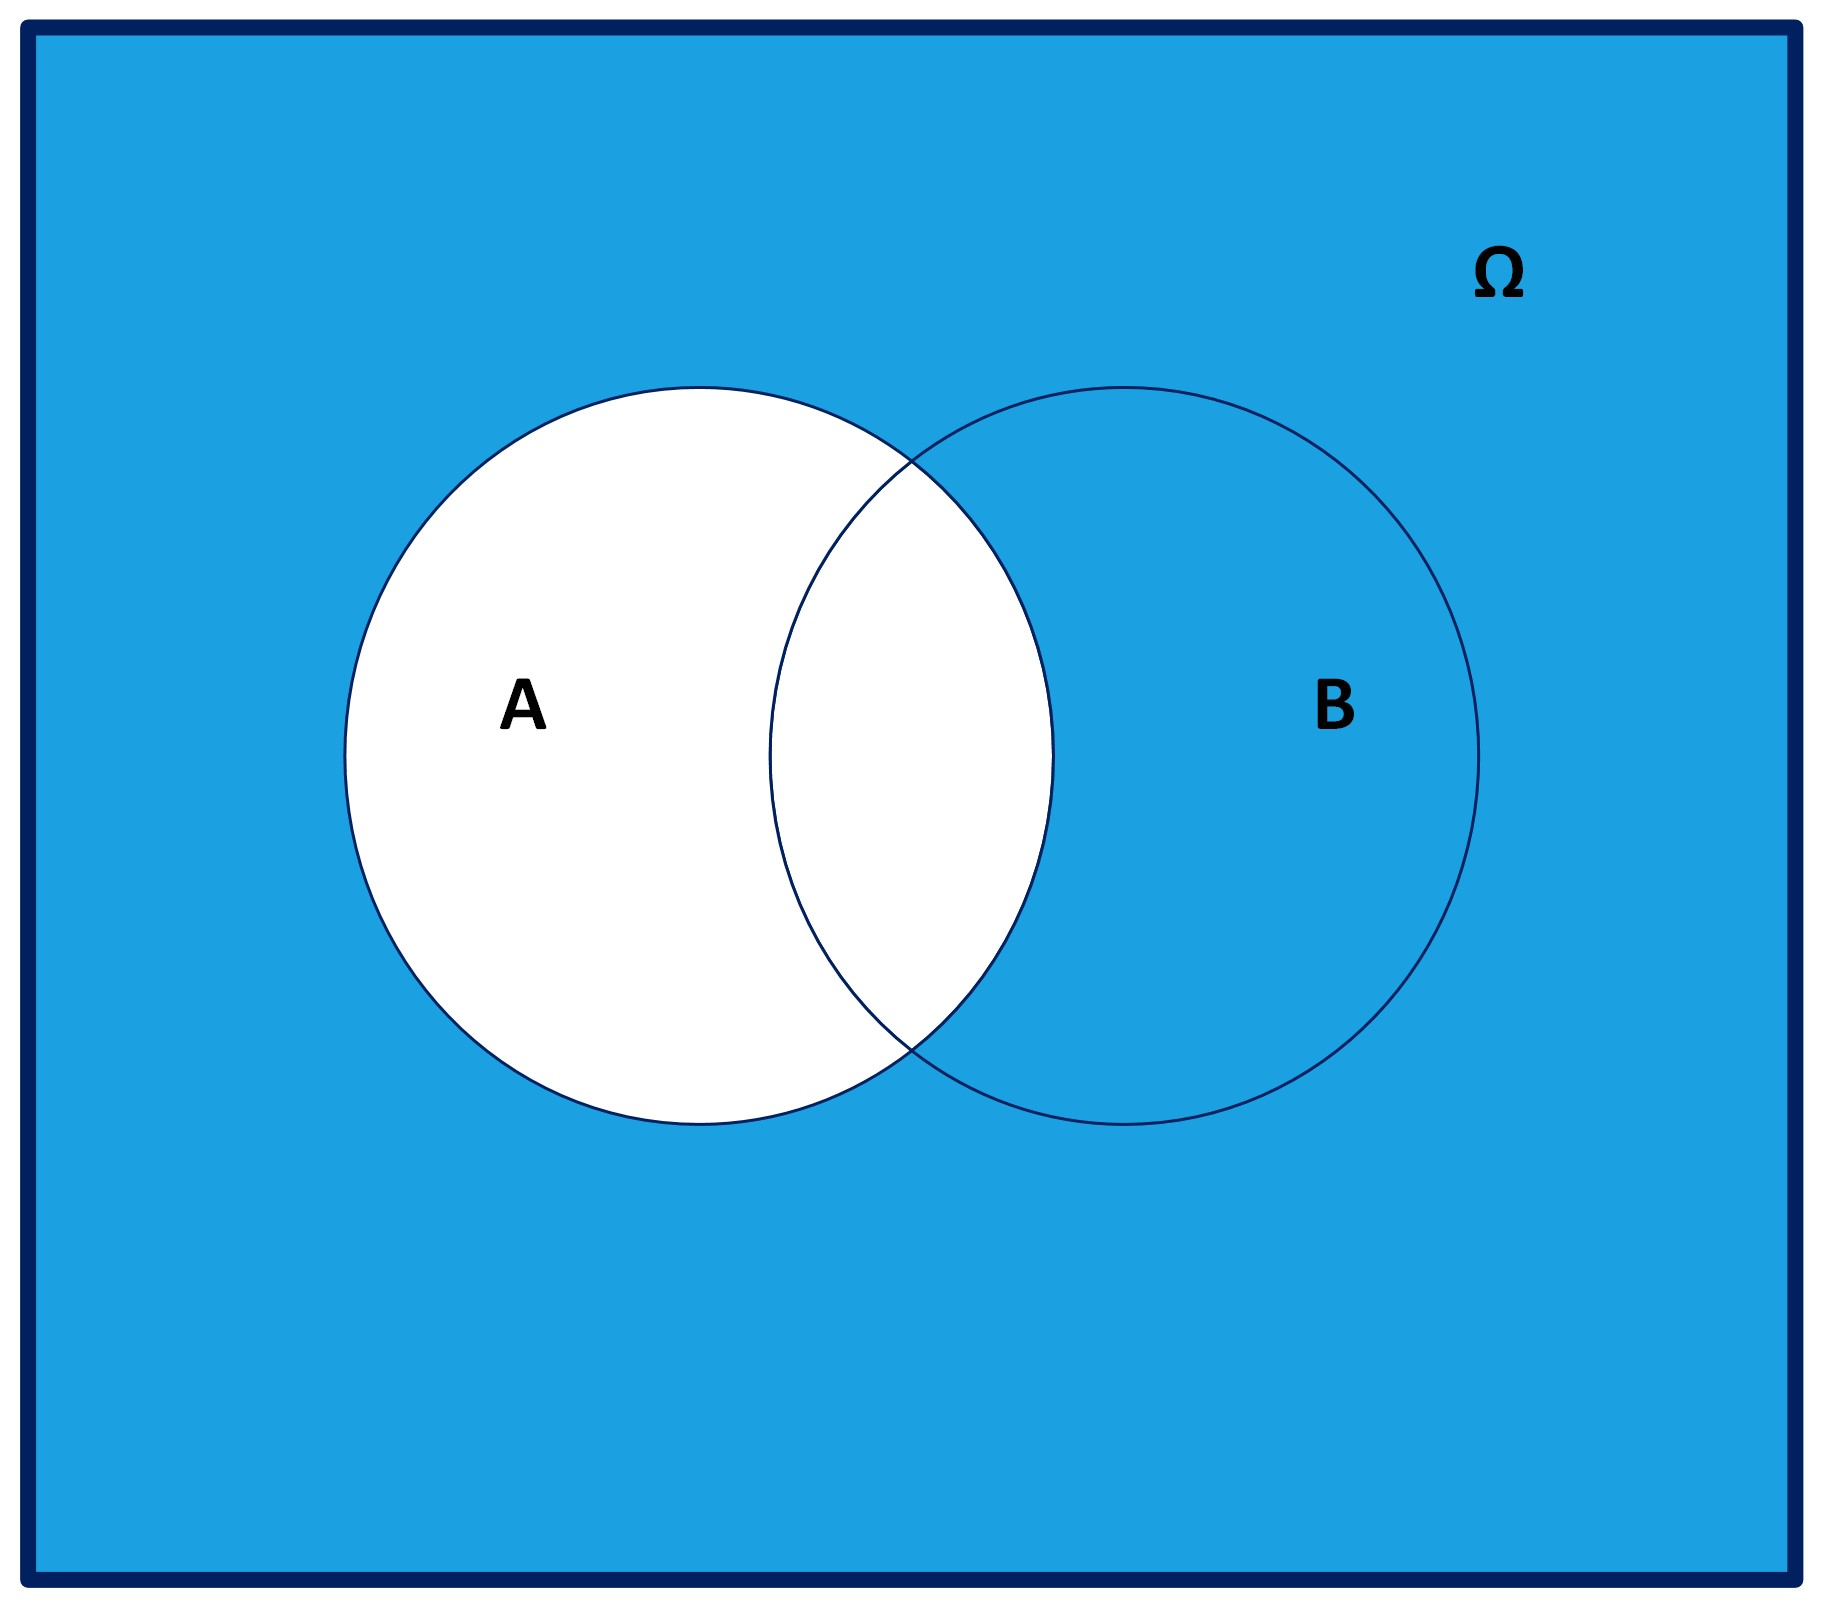
\includegraphics[width=\linewidth,height=1.5625in,keepaspectratio]{Images/venn1Ac_conB.jpeg}
&
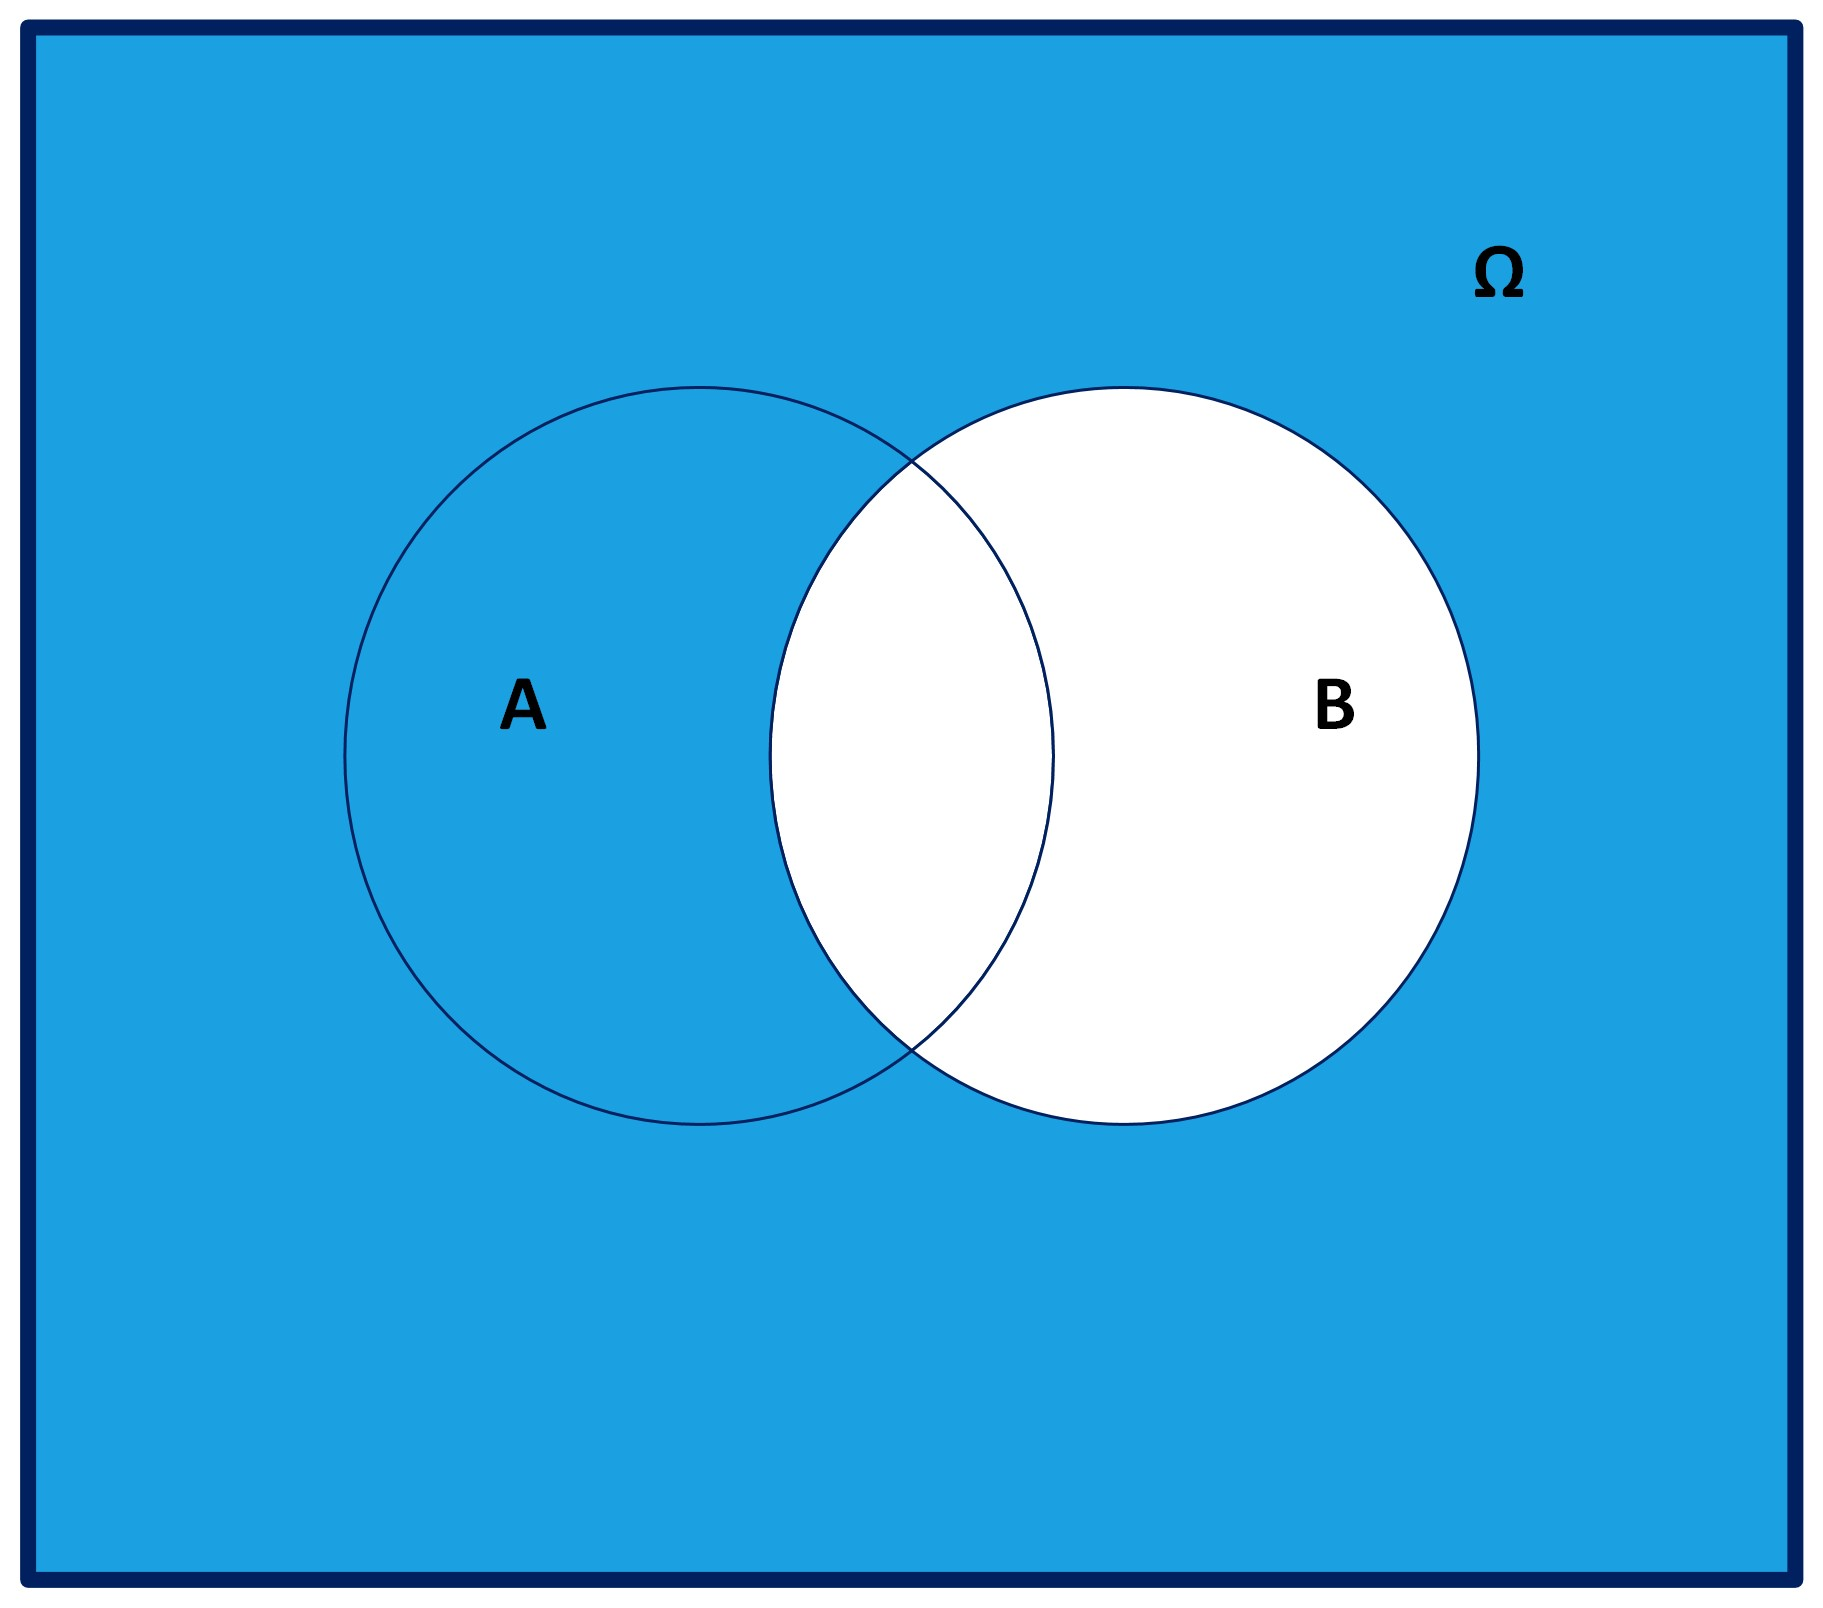
\includegraphics[width=\linewidth,height=1.5625in,keepaspectratio]{Images/venn1Bc_conA.jpeg}
&
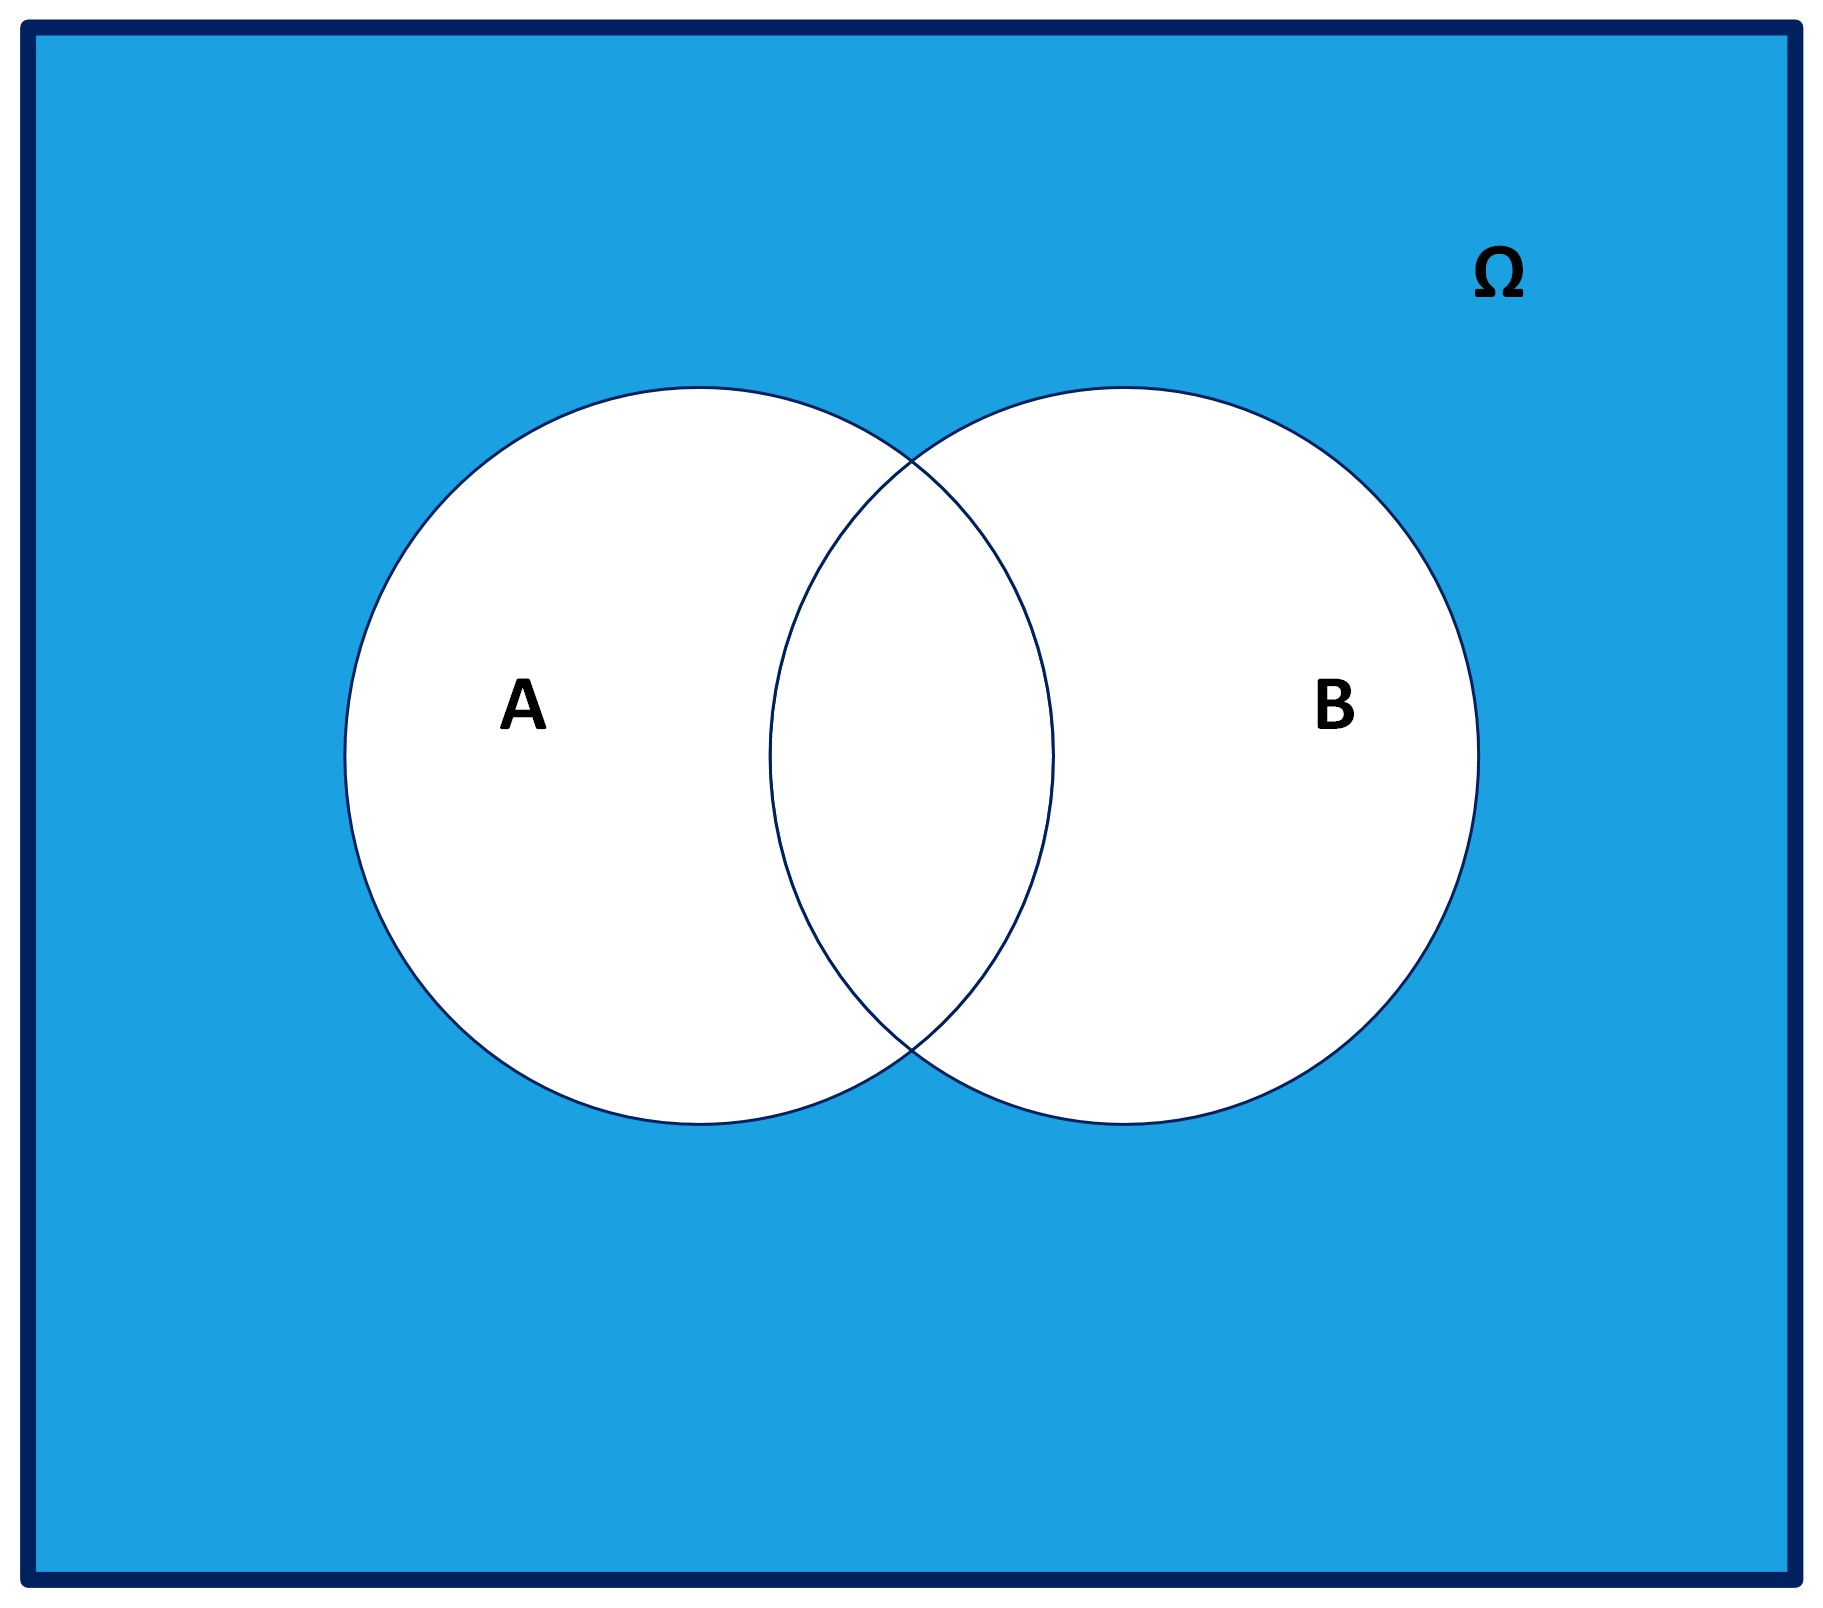
\includegraphics[width=\linewidth,height=1.5625in,keepaspectratio]{Images/venn1interseccioncomplementarios.jpeg} \\
\end{longtable}

\[(A\cap B)^c=A^c\cup B^c\]

\begin{longtable}[]{@{}
  >{\centering\arraybackslash}p{(\linewidth - 2\tabcolsep) * \real{0.5000}}
  >{\centering\arraybackslash}p{(\linewidth - 2\tabcolsep) * \real{0.5000}}@{}}
\toprule\noalign{}
\begin{minipage}[b]{\linewidth}\centering
\(A\cap B\)
\end{minipage} & \begin{minipage}[b]{\linewidth}\centering
\((A\cap B)^c\)
\end{minipage} \\
\midrule\noalign{}
\endhead
\bottomrule\noalign{}
\endlastfoot
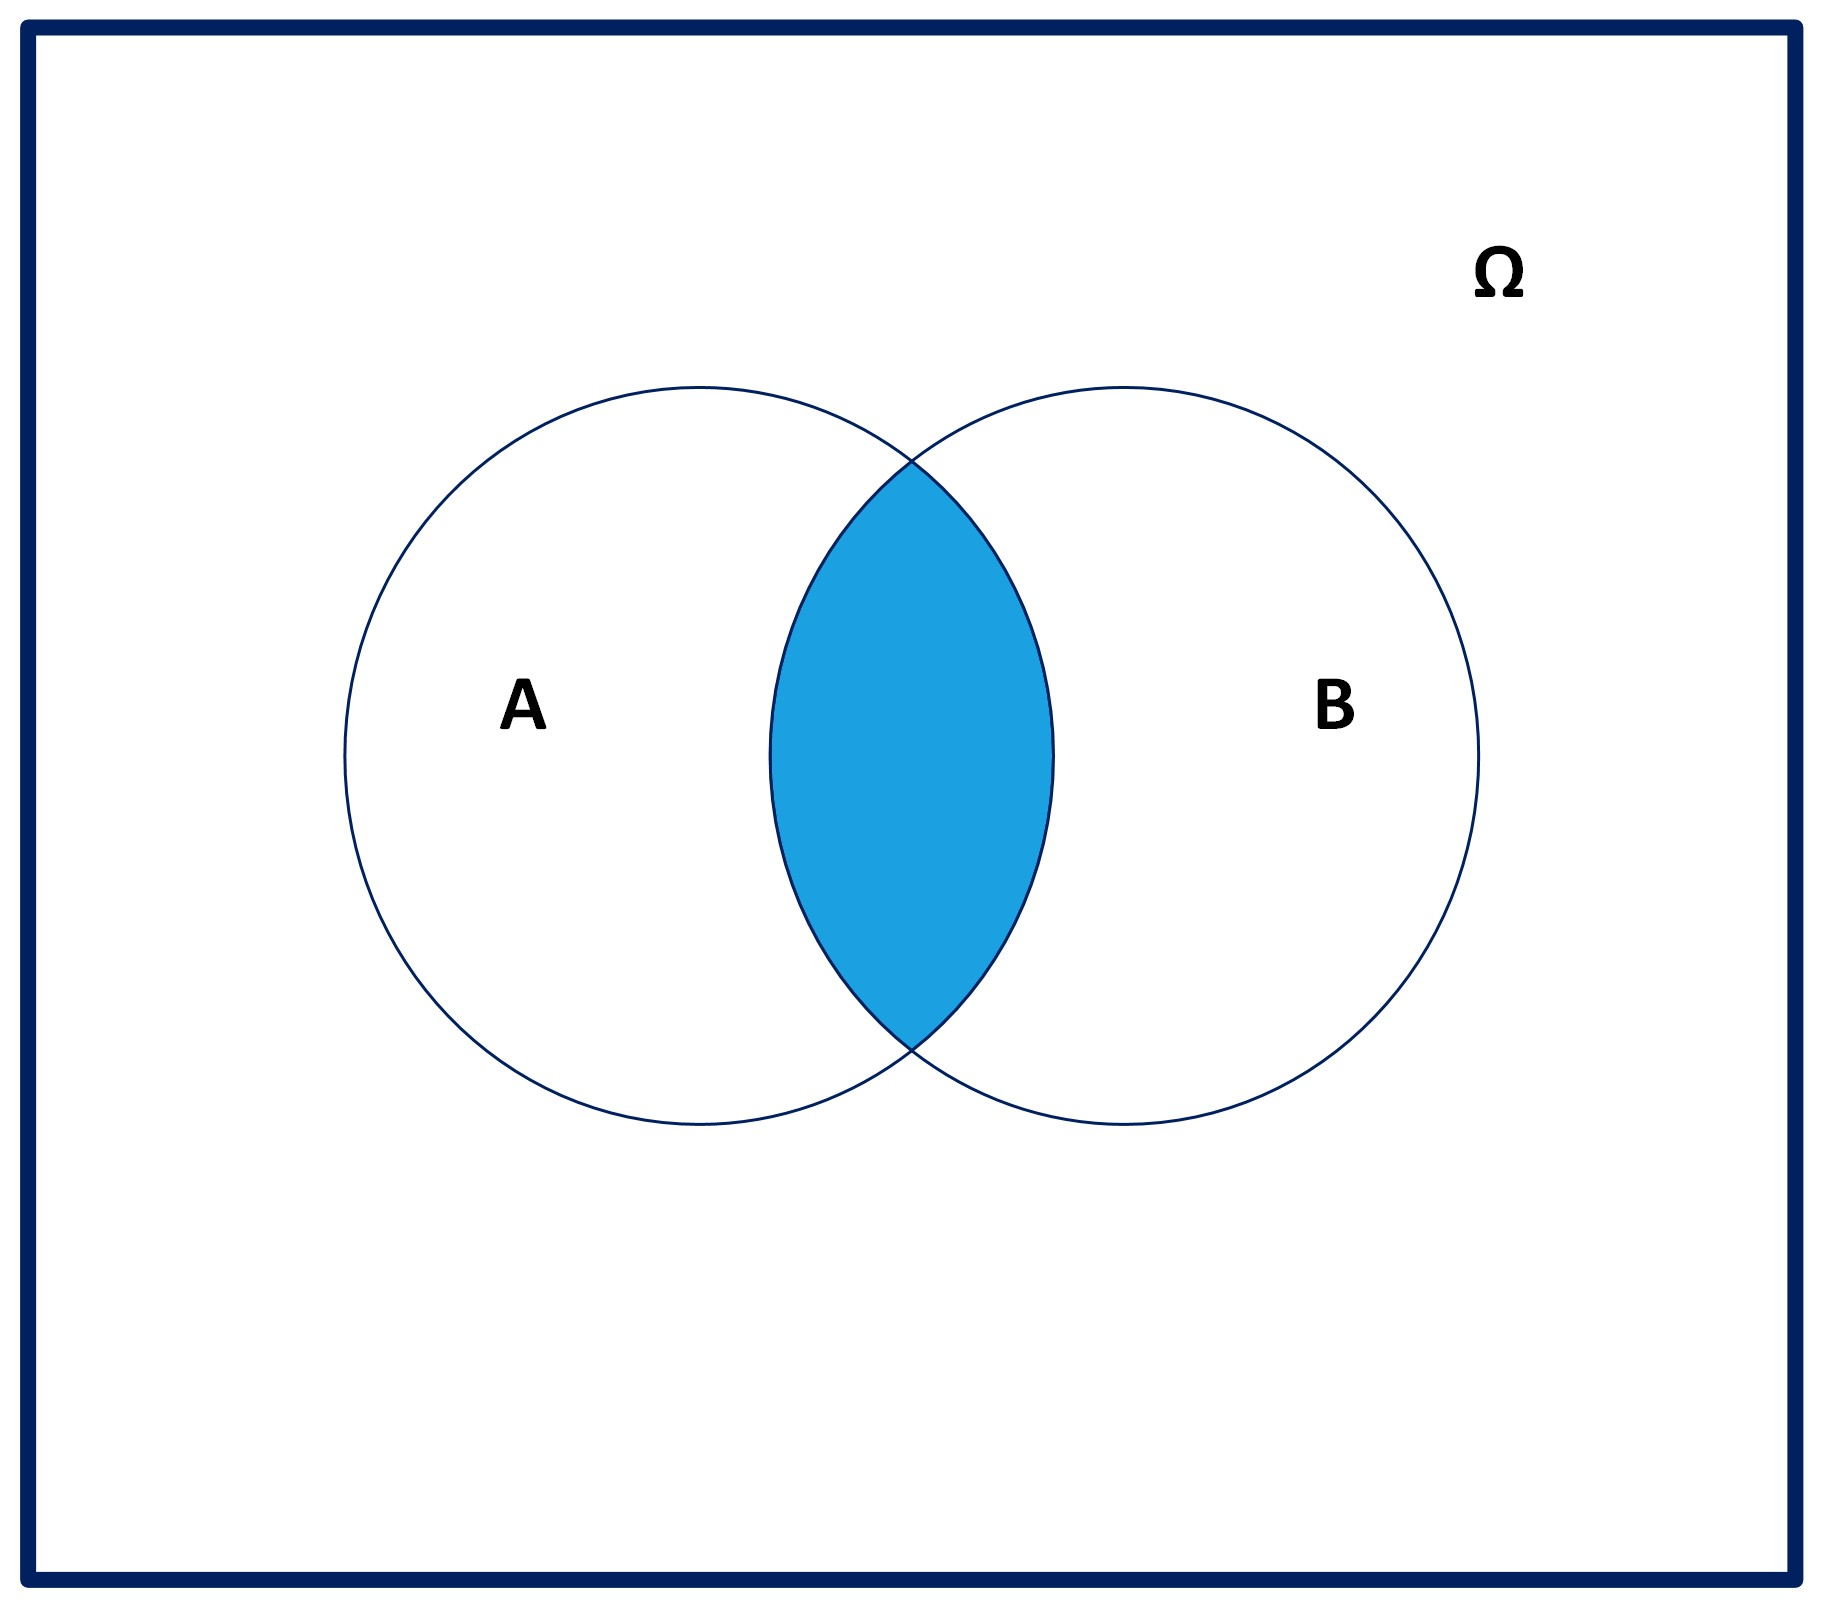
\includegraphics[width=\linewidth,height=1.5625in,keepaspectratio]{Images/venn1AyB.jpeg}
&
\includegraphics[width=\linewidth,height=1.51042in,keepaspectratio]{Images/venn1ComplementarioInterseccion.jpeg} \\
\end{longtable}

\[(A\cap B)^c=A^c\cup B^c\]

\begin{longtable}[]{@{}
  >{\centering\arraybackslash}p{(\linewidth - 4\tabcolsep) * \real{0.3333}}
  >{\centering\arraybackslash}p{(\linewidth - 4\tabcolsep) * \real{0.3333}}
  >{\centering\arraybackslash}p{(\linewidth - 4\tabcolsep) * \real{0.3333}}@{}}
\toprule\noalign{}
\begin{minipage}[b]{\linewidth}\centering
\(A^c\)
\end{minipage} & \begin{minipage}[b]{\linewidth}\centering
\(B^c\)
\end{minipage} & \begin{minipage}[b]{\linewidth}\centering
\(A^c\cup B^c\)
\end{minipage} \\
\midrule\noalign{}
\endhead
\bottomrule\noalign{}
\endlastfoot
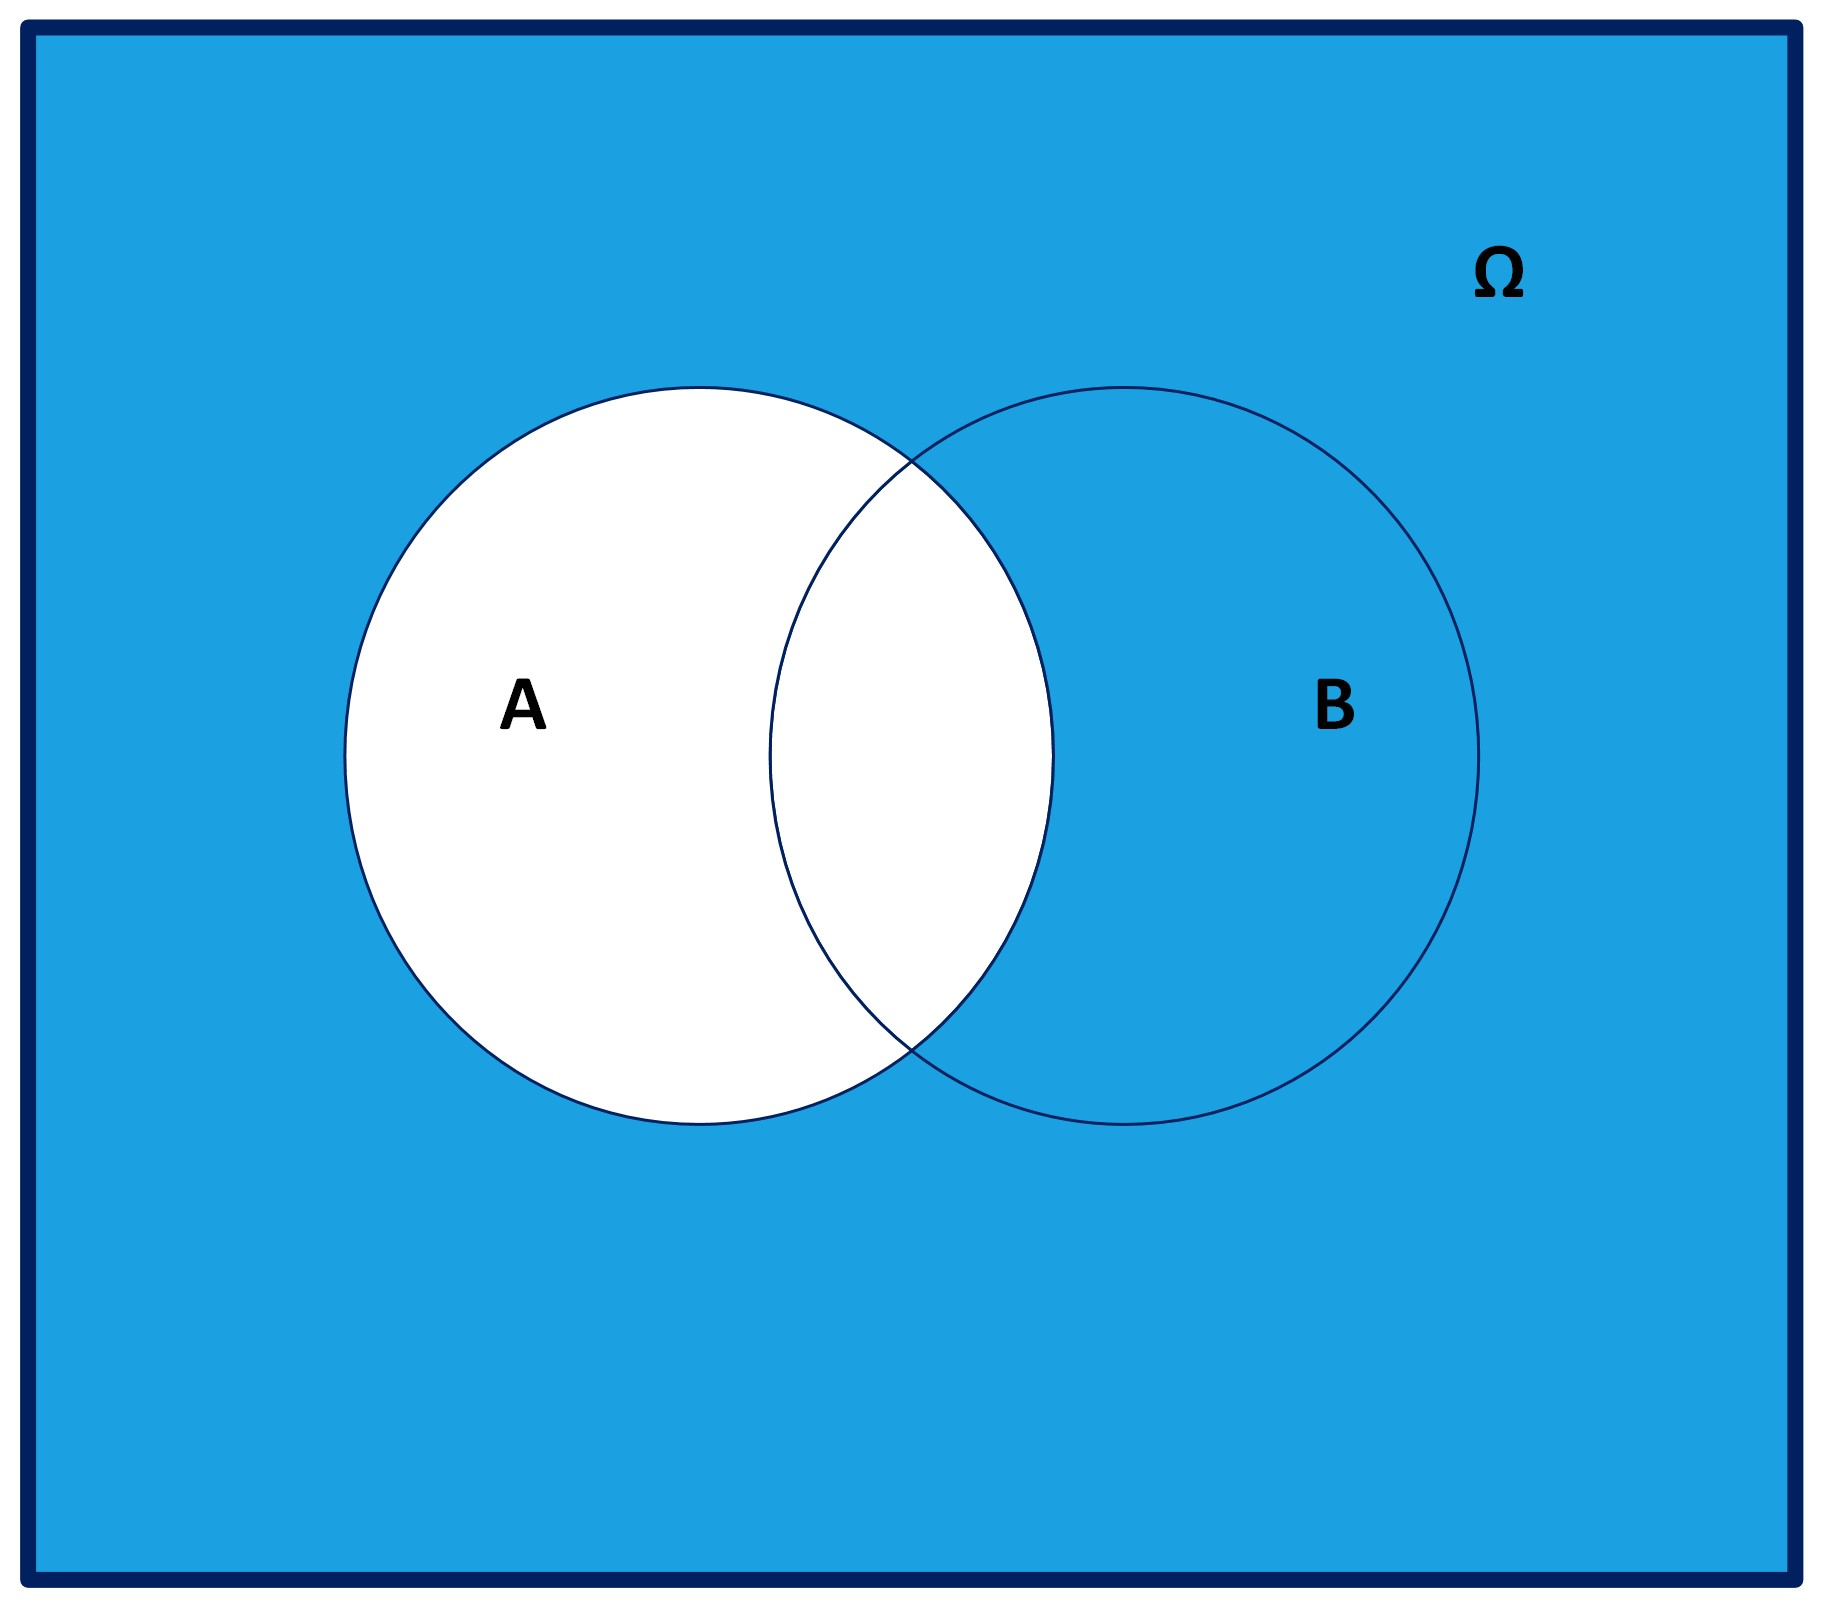
\includegraphics[width=\linewidth,height=1.5625in,keepaspectratio]{Images/venn1Ac_conB.jpeg}
&
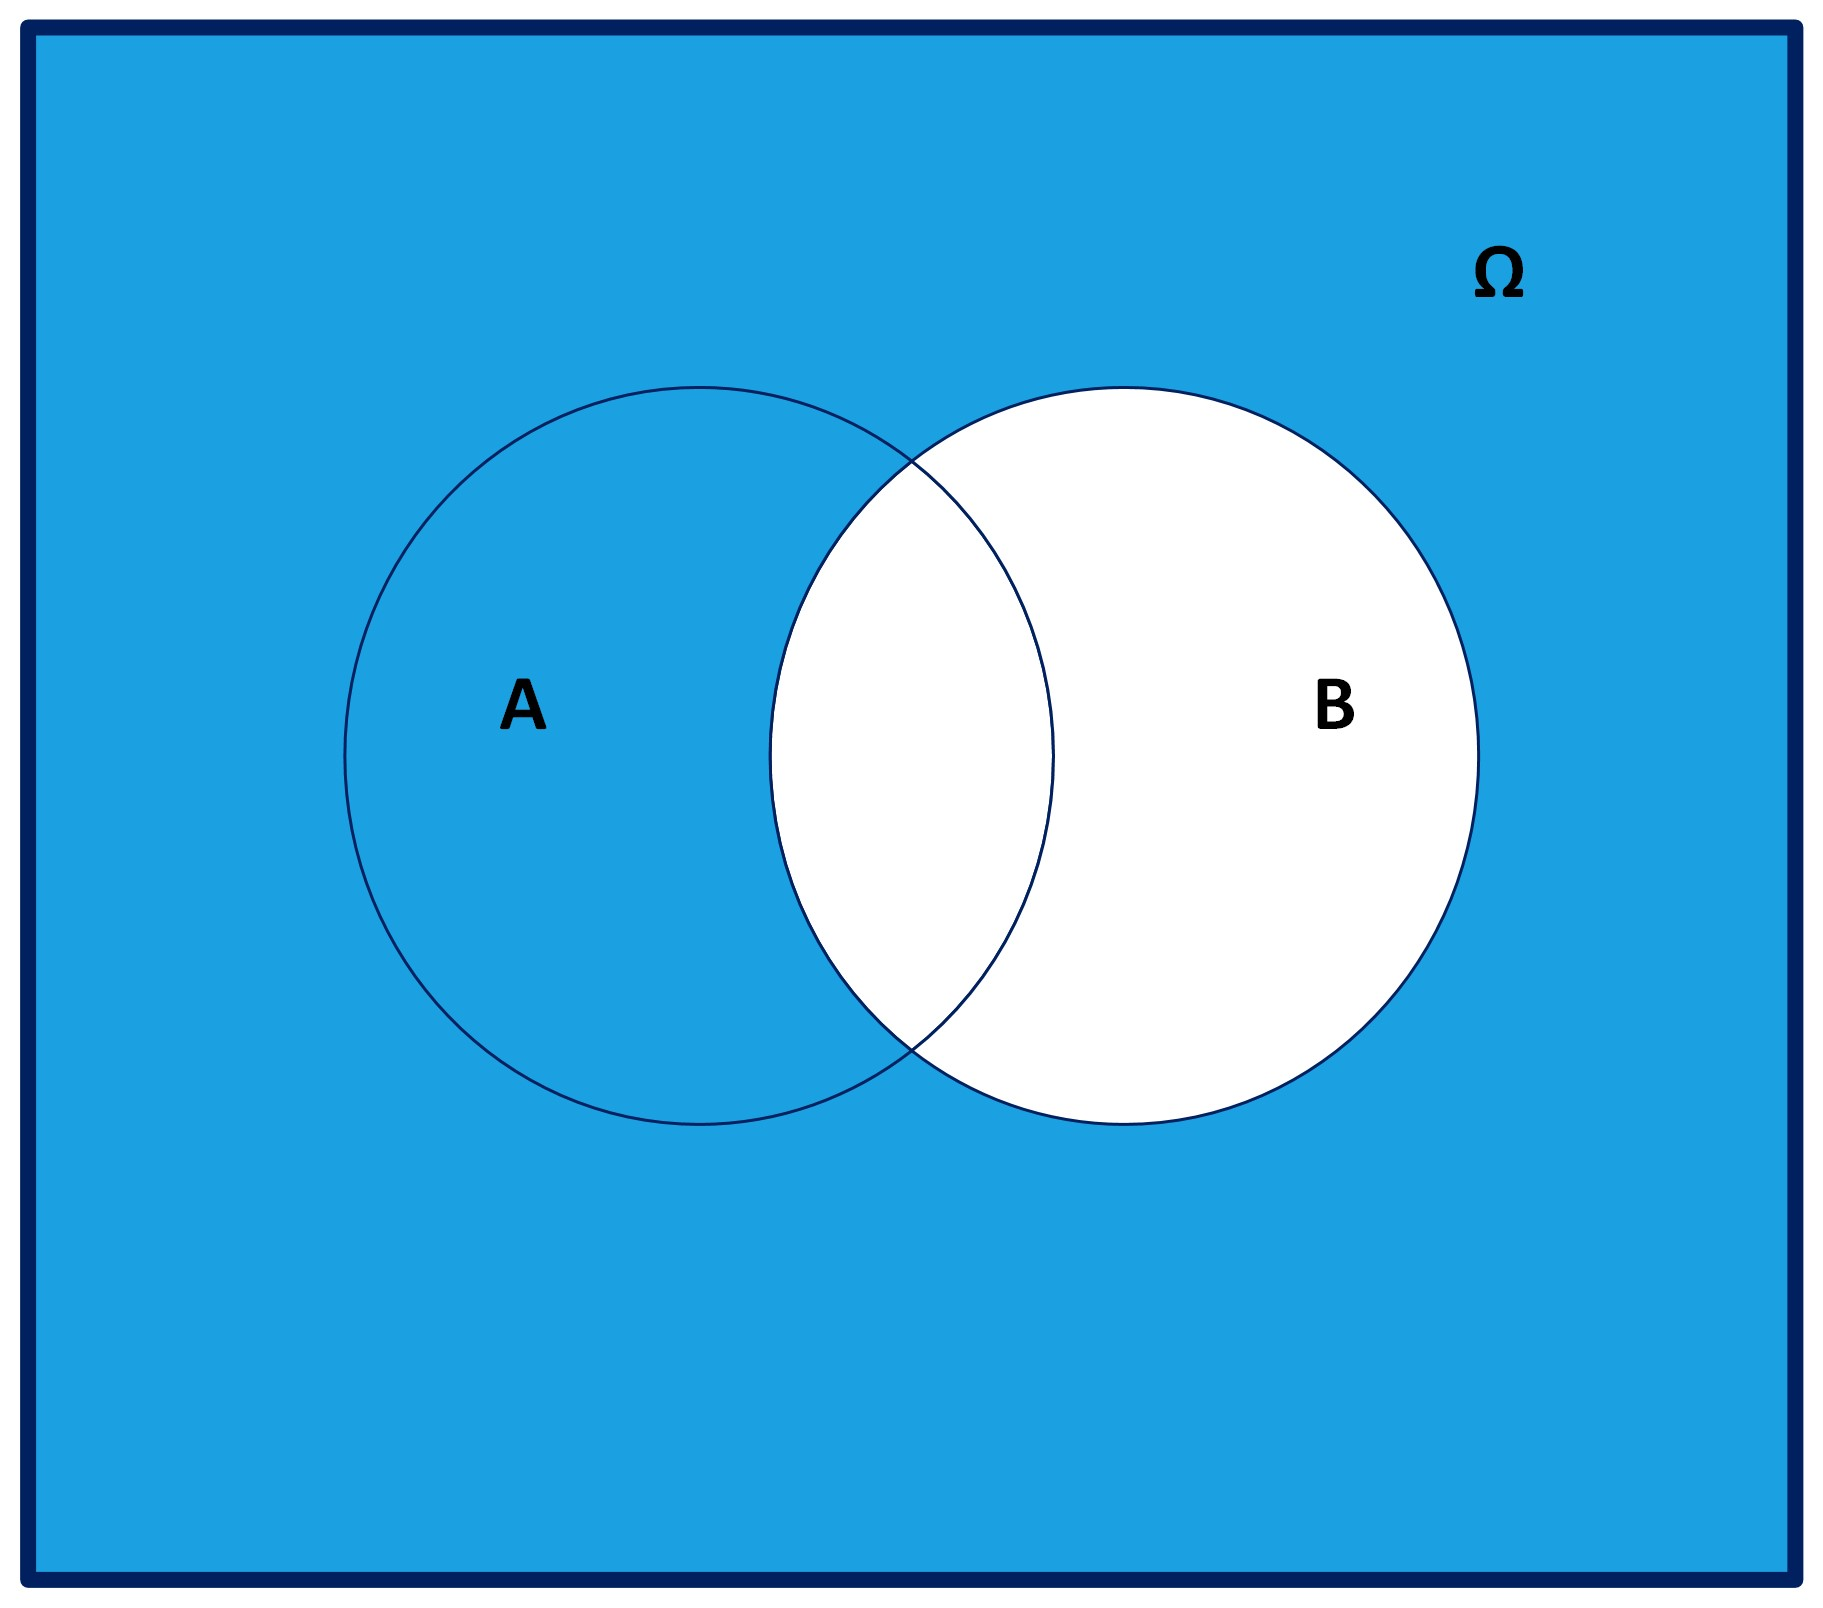
\includegraphics[width=\linewidth,height=1.5625in,keepaspectratio]{Images/venn1Bc_conA.jpeg}
&
\includegraphics[width=\linewidth,height=1.51042in,keepaspectratio]{Images/venn1ComplementarioInterseccion.jpeg} \\
\end{longtable}

\section{Definición de
probabilidad}\label{definiciuxf3n-de-probabilidad}

La probabilidad de un suceso es una puntuación (\emph{score}) numérico
entre 0 y 1 que mide la verosimilitud de que este evento se produzca.

Esta verosimilitud puede estar justificada por:

\begin{itemize}
\item
  Estimación personal
\item
  Estimación de expertos
\item
  La frecuencia con la que se da
\item
  Cálculo formal
\end{itemize}

Definición formal de probabilidad

Sea \(\Omega\) el espacio muestral de un experimento aleatorio.
Supongamos que el número de posibles resultados, por el momento, es
finito.

Una probabilidad sobre \(\Omega\) es una aplicación
\(P:\mathcal{P}(\Omega)\to [0,1]\) con las siguientes propiedades:

\begin{enumerate}
\def\labelenumi{\arabic{enumi}.}
\tightlist
\item
  \(0\leq P(A)\leq 1\), para todo suceso \(A\).
\item
  \(P(\Omega)=1\).
\item
  Si \(\{A_1,A_2,\ldots,A_n\}\) son sucesos disjuntos dos a dos,
  entonces
\end{enumerate}

\[
P(A_1\cup A_2\cup \cdots \cup A_n)=P(A_1)+P(A_2)+\cdots +P(A_n)
\]

Si \(a\in \Omega\) es un suceso elemental cometeremos el abuso de
notación de poner \(P(a)\) en lugar de \(P(\{a\})\).

Veamos un ejemplo real de cómo se calcula la probabilidad de un suceso.

Ejemplo

En la página de la
\href{http://www.donasang.org/que-es-la-sang/es_frequencies-dels-diferents-grups.html}{Fundación
Banco de Sangre y Tejidos de las Islas Baleares (17-08-2023)} podemos
encontrar información sobre los porcentajes de tipos de sangre de los
donantes de las Islas Baleares:

\[A: 46\%;\  B: 7.5\%;\  AB: 3.5\%;\  O: 43\%.\]

¿Cuál es la probabilidad de que un balear donante de sangre no sea del
tipo O?

\textbf{Experimento aleatorio:} tipo de sangre de un paciente humano:

\[\Omega=\{\mbox{A,B,AB,O}\}\]

\textbf{Probabilidad} de un suceso: se asimila al porcentaje observado
de individuos.

\textbf{Suceso:} \(\{\mbox{O}\}^c=\{\mbox{A,B,AB}\}\).

\[P(\{\mbox{O}\}^c)\!=\!P(\{\mbox{A,B,AB}\})\!=\!
P(\mbox{A})+P (\mbox{B})+P(\mbox{AB})\!=\!0.57.\]

Necesitaremos tener propiedades y fórmulas prácticas para poder calcular
probabilidades de sucesos más complejos. Veamos algunas de ellas.

Propiedades básicas de la probabilidad

\begin{itemize}
\item
  \(P(\emptyset)=0\).
\item
  \(\scriptsize{P(A-B)=P(A)-P(A\cap B)}\) porque
  \(\scriptsize{P(A)=P(A-B)+P(A\cap B)}\).
\end{itemize}

\begin{center}
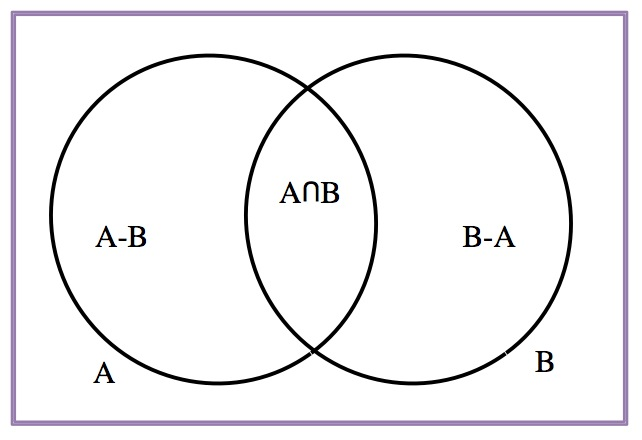
\includegraphics[width=0.3\linewidth,height=\textheight,keepaspectratio]{Images/proba1dibujos/A-B.jpg}
\end{center}

\begin{itemize}
\item
  Si \(B\subseteq A\), entonces \(0\leq P(B)\leq P(A)\).
\item
  \(P(A^c)=1-P(A)\).
\end{itemize}

Una identidad muy utilizada es la de la probabilidad de la unión de dos
sucesos cualesquiera.

La Probabilidad de la unión de dos sucesos

\(P(A\cup B)=P(A)+P(B)-P(A\cap B)\)

\begin{center}
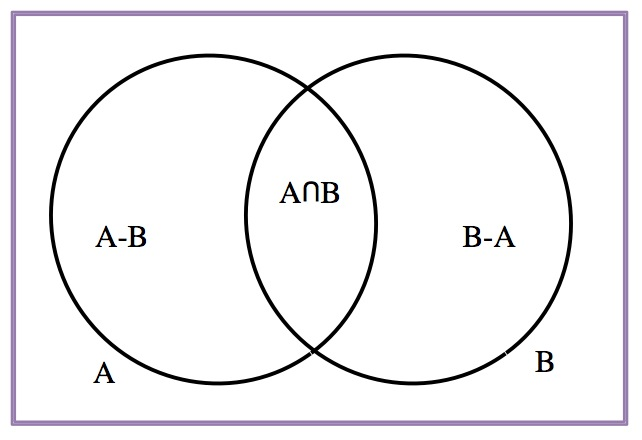
\includegraphics[width=0.6\linewidth,height=\textheight,keepaspectratio]{Images/proba1dibujos/A-B.jpg}
\end{center}

La demostración analítica de esta propiedad es la siguiente:

\begin{eqnarray*}
P(A)+P(B)-P(A\cap B) &=& P(A-B)+P(A\cap B)\\ 
& & +P(B-A)+ P(A\cap  B)-P(A\cap  B)\\
&=& P(A-B)+P(A\cap B)+ P(B-A) \\
&=& P(A\cup B).\\
\end{eqnarray*}

Probabilidad de la unión de \(n\) conjuntos

Sean \(A_1, A_2,\ldots A_n\) sucesos. Entonces:

\[
P(\cup_{i=1}^n A_i)=\sum_{i=1}^n P(A_i)-\sum_{1\leq i<j\leq n}P(A_i\cap A_j)+\cdots +(-1)^{n-1}P(A_1\cap A_2\cap \cdots \cap A_n).
\]

La demostración es sencilla mediante inducción: partimos del caso base
de dos sucesos, suponemos que es cierta para \(n\) sucesos y luego la
extendemos al caso de \(n+1\) sucesos.

Como comprobación, consideremos un ejemplo genérico con tres sucesos.

\(A=\{1,4,5,6\}\), \(B=\{2,4,6,7\}\) y \(C=\{3,5,6,7\}\). En este caso
la fórmula nos da

\[
P(A\cup B\cup C)=  P(A)+P(B)+P(C)-P(A\cap B)-P(A\cap C)
-P(B\cap C)+P(A\cap B\cap C).
\]

Gráficamente tenemos esta situación:

\begin{center}
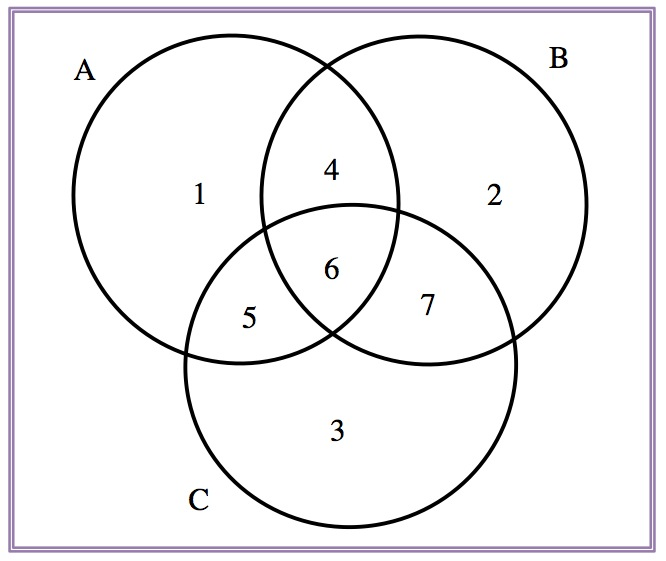
\includegraphics[width=0.3\linewidth,height=\textheight,keepaspectratio]{Images/proba1dibujos/tresconjunts.jpg}
\end{center}

Ahora podemos comprobar la fórmula para este caso.

\begin{eqnarray*}
P(A\cup B\cup C)&=&P(A)+P(B)+P(C)-P(A\cap B) \\
  & & - P(A\cap C)-P(B\cap C)+P(A\cap B\cap C).\\
\end{eqnarray*}

Efectivamente tenemos que:

\[P(A\cup B\cup C)=P(1)+P(2)+P(3)+P(4)+P(5)+P(6)+P(7).\]

Una de las formas más intuitiva de asignación de probabilidades es hacer
el cociente entre los casos favorables a que acontezca el vento y los
casos posibles del experimento; la llmadad fórmula de Laplace.

Propiedad

\begin{itemize}
\item
  En general dado un suceso \(A=\{a_1,a_2,\ldots,a_k\}\), entonces \[
  P(A)=P(a_1)+P(a_2)+\cdots+P(a_k).
  \]
\item
  \textbf{Fórmula de Laplace}: Si todos los sucesos elementales tienen
  la misma probabilidad, \[
  P(A)=\frac{|A|}{|\Omega|}\Big(=\frac{\mbox{casos favorables}}{\mbox{casos posibles}}\Big).
  \]
\end{itemize}

En el procesamiento del lenguaje se suelen estudiar las frecucias de
plabaras o letras de un determinado idioma. Veamos un ejemplo sobre las
frecuencias de las vocales en castellano.

Ejemplo: Frecuencia de vocales

Los porcentajes de vocales de un determinado idioma (de alfabeto latino)
según la
\href{https://es.wikipedia.org/wiki/Frecuencia_de_aparici\%C3\%B3n_de_letras}{Wikipedia}
son:

\[A: 18.7\%;\ E: 26.1\%;\ I: 25.7\%;\ O: 24.4\%;\ U: 5.1\%.\]

¿Cuál es la probabilidad que una vocal escogida al azar de este idioma
sea una E o una O?

El espacio muestral del experimento es \(\Omega=\{A,E,I,O,U\}\).

El suceso que deseamos analizar es \(\{E,0\}\).

Y su probabilidad es

\[P(\{E,O\})=P(E)+P(O)=0.261+0.244=0.505.\]

Otro ejemplo en este caso es sobre un test de drogas en el que se
analiza la presencia de cocaína y cannabis en la sangre de los
conductores, inspirado en un caso real.

Ejemplo: Consumo de drogas

Segun un árticulo de
\href{https://elpais.com/politica/2019/01/02/actualidad/1546426491_623324.html}{El
País}, en un control especial de la policía el \(0.1\%\) de todos los
conductores analizados en un control de tráfico dan positivo en un el
test en cocaína, y el \(1\%\) da positivo en cannabis. Un \(1.05\%\) da
positivo en alguno de los dos test.

\textbf{Pregunta}: ¿Cuál es la probabilidad que un individuo analizado
en el control de drogas escogido al azar no de positivo en ninguno de lo
dos test?

Los sucesos elementales del enunciado del problema son:

\begin{itemize}
\tightlist
\item
  \(A\): dar positivo en cocaína; \(P(A)=0.001.\)
\item
  \(B\): dar positivo en cannabis; \(P(B)=0.01.\)
\end{itemize}

En este caso nos interesa estudiar los sucesos:

\begin{itemize}
\tightlist
\item
  \(A\cup B\): dar positivo en alguno de los dos test;
  \(P(A\cup B)=0.0105.\)
\item
  \((A\cup B)^c\): no dar positivo en ninguno de los test,por tanto:
\end{itemize}

\[P((A\cup B)^c)=1-P(A\cup B)=1-0.0105=0.9895.\]

\textbf{Pregunta}: ¿Cuál es la probabilidad que un analizado al azar de
positivo en los dos test en cocaína y cannabis?

Los sucesos elementales son:

\begin{itemize}
\tightlist
\item
  \(A\): dar positivo en cocaína; \(P(A)=0.001.\)
\item
  \(B\): dar positivo en cannabis; \(P(B)=0.01.\)
\end{itemize}

En este caso nos interesa estudiar los sucesos:

\begin{itemize}
\tightlist
\item
  \(A\cup B\): dar positivo en algún de los dos test;
  \(P(A\cup B)=0.0105.\)
\item
  \(A\cap B\): dar positivo en los dos test
\end{itemize}

de donde, por tanto:

\[\begin{array}{rl}
{P(A\cap B)} &{=P(A)+P(B)-P(A\cup B)}\\ &{=0.001+0.01-0.0105=0.0005}.
\end{array}\]

\textbf{Pregunta}: ¿Cuál es la probabilidad de que un conductor
analizado de positivo en cocaína pero no en cannabis?

Los sucesos elementales son:

\begin{itemize}
\tightlist
\item
  \(A\): dar positivo en cocaína; \(P(A)=0.001.\)
\item
  \(B\): dar positivo en cannabis; \(P(B)=0.01.\)
\end{itemize}

En este caso nos interesa estudiar los sucesos:

\begin{itemize}
\tightlist
\item
  \(A\cap B\): dar positivo en los dos test; \(P(A\cap B)=0.0005.\)
\item
  \(A-B\): dar positivo en cocaína pero no en cannabis, por lo tanto
  tenemos que :
\end{itemize}

\[P(A-B) =P(A)-P(A\cap B) =0.001-0.0005=0.0005.\]

\section{Probabilidad condicionada}\label{probabilidad-condicionada}

Probabilidad condicionada

Dados dos sucesos \(A\) y \(B\), con \(P(A)>0\), la probabilidad
\(P(B|A)\) de \(B\) condicionado a \(A\) es la probabilidad

\begin{itemize}
\tightlist
\item
  de que suceda \(B\) suponiendo que pasa \(A\),
\item
  de que si pasa \(A\), entonces suceda \(B\),
\item
  de que un resultado de \(A\) también pertenezca a \(B\).
\end{itemize}

Se calcula a través de la definición:

\[
P(B|A)=\frac{P(A\cap B)}{P(A)}.
\]

Ejemplo

En una clase de 20 hombres y 30 mujeres, 15 hombres y 18 mujeres llevan
gafas. Contestemos las siguientes preguntas:

¿Cuál es la probabilidad de que un alumno lleve gafas?

\[
\frac{33}{50}
\]

¿Cuál es la probabilidad de que un alumno sea mujer y lleve gafas?

\[
\frac{18}{50}
\]

¿Cuál es la probabilidad de que un chica lleve gafas?

\[
\frac{18}{30}=\frac{18/50}{30/50}=\frac{P(\mbox{mujer  y gafas})}{P(\mbox{mujer})}.
\]

Si escogemos un estudiante al azar ¿Cuál es la probabilidad que si es
mujer, entonces lleve gafas?

\[
\frac{18}{30}.
\]

¿Cuál es la probabilidad de que un alumno que lleve gafas sea mujer?

\[
\frac{18}{33}=\frac{18/50}{33/50}=\frac{P(\mbox{mujer y gafas})}{P(\mbox{gafas})}.
\]

Si escogemos un estudiante al azar ¿Cuál es la probabilidad de que si
lleva gafas, entonces sea mujer? \[
    \frac{18}{33}
    \]

¡Atención!

Hay que distinguir bien entre

\begin{itemize}
\tightlist
\item
  \(P(A\cap B)\): probabilidad de \(A\) \(\color{red}{\text{y}}\) \(B\).
\end{itemize}

\emph{Probabilidad de que sea mujer y lleve gafas.}

\begin{itemize}
\tightlist
\item
  \(P(A|B)\): probabilidad de que \(\color{red}{\text{si}}\) pasa \(B\),
  \(\color{red}{\text{entonces}}\) pase \(A\).
\end{itemize}

\emph{Probabilidad de que, si es mujer, lleve gafas.}

Cuando utilizamos probabilidad condicional \(P(A|B)\) estamos
restringiendo el espacio muestral a \(B\).

\subsection{Probabilidad condicionada.
Propiedades}\label{probabilidad-condicionada.-propiedades}

La probabilidad condicionada es una probabilidad, en el setido de la
siguiente propiedad.

Propiedad

Sea \(A\subseteq \Omega\) un suceso tal que \(P(A)>0\), entonces

\[
\begin{array}{rccl}
P(-|A):& \mathcal{P}(\Omega) & \to & [0,1]\\
&B & \mapsto & P(B|A).
\end{array}
\] satisface las propiedades de las probabilidades, como por ejemplo:

\[
\begin{array}{l}
P(B^c|A)=1-P(B|A),\\
P(B_1\cup B_2|A)=P(B_1|A)+P(B_2|A)-P(B_1\cap B_2|A).
\end{array}
\]

También se cumpliran el resto de propiedades miestras condiciones todas
ellas al mismo suceso \(A\).

Ejercicio

Escribid el resto de propiedades que cumpliría una probabilidad
condicionada al evento \(A\).

Veamos un ejemplo donde se aplica la probabilidad condicionada, en este
caso, para calcular la probabilidad de que un adulto sea hipertenso,
dado que cree que lo es.

Ejemplo

Un 15\% de los adultos son hipertensos, un 25\% de los adultos creen que
son hipertensos, y un 9\% de los adultos son hipertensos y creen que lo
son.

Si un adulto cree que es hipertenso, ¿cuál es la probabilidad que lo
sea?

Sean los sucesos

\begin{itemize}
\tightlist
\item
  \(A\): ser hipertenso, \(P(A)=0.15\) ,
\item
  \(B\): creer ser hipertenso, \(P(B)=0.25\),
\end{itemize}

Ahora podemos definir el suceso:

\begin{itemize}
\tightlist
\item
  \(A\cap B\): ser hipertenso y creerlo, \(P(A\cap B)=0.09\).
\end{itemize}

de donde, la probabilidad condicionada de ser hipertenso creyéndonos que
lo somos es:

\[\scriptsize P(A|B)=\dfrac{P(A\cap B)}{P(B)}=\dfrac{0.09}{0.25}=0.36.\]

Otra pregunta es, si un adulto es hipertenso, ¿cuál es la probabilidad
que crea que lo es?

Si tenemos los sucesos:

\begin{itemize}
\tightlist
\item
  \(A\): ser hipertenso,
\item
  \(B\): creer ser hipertenso
\end{itemize}

entonces buscamos la probabilidad \(P(B|A)\):

\[
\begin{array}{rl}
P(B|A) & =\dfrac{P(A\cap B)}{P(A)}=\dfrac{0.09}{0.15}=
0.6
\end{array}
\]

Ejemplo

Otro ejemplo de probabilidad condicionada en este caso un ejemplo simple
de dígito de control de error.

Un dígito de control de error toma el valor 0 en el 99\% de los casos en
que hay un error. Si la probabilidad de error en un mensaje es del
\(0.5\%\). ¿cuál es la probabilidad de que el mensaje sea erróneo y el
código de error tenga valor 0?

\begin{itemize}
\tightlist
\item
  \(B\): mensaje con error; \(P(B)=0.005\),
\item
  \(A\): código de error vale 0,
\item
  \(P(A|B)=0.99\),
\end{itemize}

entonces: \[P(A\cap B)=P(B)\cdot P(A|B)=0.005\cdot 0.99=0.00495.\]

La probabilidad condicional también es útil en la resolución de
problemas de clasificación, como el siguiente ejemplo.

Ejemplo: SPAM

Un 50\% de correos recibidos en un servidor llevan adjuntos y un 65\%
son publicidad no deseada (SPAM). Sólo un 15\% de estos correos no
llevan adjuntos y no son SPAM.

\begin{itemize}
\tightlist
\item
  ¿Cuál es la probabilidad que un correo lleve adjunto si es SPAM?
\item
  ¿Cuál es la probabilidad que un correo \textbf{no} tenga adjuntos si
  \textbf{no} es SPAM?
\item
  ¿Cuál es la probabilidad que un correo lleve adjunto si es SPAM?
\end{itemize}

Asignemos sucesos y probabilidades

\begin{itemize}
\tightlist
\item
  \(A\): llevar adjuntos; \(P(A)=0.5\), - \(S\): SPAM; \(P(S)=0.65\), -
  \(A^c\cap S^c=(A\cup S)^c\): no llevar adjunto y no ser SPAM;
  \(P((A\cup S)^c)=0.15\),
\end{itemize}

\[P(A|S)=\dfrac{P(A\cap S)}{P(S)}=?\]

\begin{itemize}
\item
  ¿Cuál es la probabilidad que un correo lleve adjunto si es SPAM?
\item
  \(P(A)=0.5, P(S)=0.65, P(A^c\cap S^c)=P((A\cup S)^c)=0.15\),
\item
  \(P(A\cup S)=1-P((A\cup S)^c)=0.85\),
\item
  \(P(A\cap S)=P(A)+P(S)-P(A\cup S)=0.3\),
\end{itemize}

\[P(A|S)=\dfrac{P(A\cap S)}{P(S)}=\dfrac{0.3}{0.65}\approx 0.46.\]

\begin{itemize}
\item
  Otra pregunta es ¿Cuál es la probabilidad de que un correo no lleve
  adjuntos si no es SPAM?
\item
  \(P(A)=0.5, P(S)=0.65, P(A^c\cap S^c)=P((A\cup S)^c)=0.15.\)
\end{itemize}

\[P(A^c|S^c)=\dfrac{P(A^c\cap S^c)}{P(S^c)}=\dfrac{P(A^c\cap S^c)}{1-P(S)}=\dfrac{0.15}{0.35}\approx 0.43.\]

\section{Teorema de la probabilidad
total}\label{teorema-de-la-probabilidad-total}

Teorema de la probabilidad total

Dados dos sucesos \(A\) y \(B\) se tiene que

\[
\begin{array}{rl}
P(B)&= P(B\cap A) +P(B\cap A^c)\\
& =P(A)\cdot P(B|A)+ P(A^c)\cdot P(B|A^c).
\end{array}
\]

Vamos a generalizar el resultado anterior a una colección de sucesos
\(A_1,A_2,\ldots,A_n\) que forman una partición del espacio muestral
\(\Omega\).

Partición del espacio espacio muestral

Los sucesos \(A_1,A_2,\ldots, A_n\) son una \textbf{partición} del
espacio muestral \(\Omega\) de un determinado experimento aleatorio, si
cumplen las condiciones siguientes:

\begin{enumerate}
\def\labelenumi{\arabic{enumi}.}
\tightlist
\item
  \(A_1\cup A_2\cup\ldots\cup A_n=\Omega\),
\item
  \(A_1,A_2,\ldots,A_n\) son incompatibles dos a dos
  (\(A_i\cap A_j=\emptyset\)).
\end{enumerate}

Ahora podemos volver a enunciar el teorema anterior pero en esta ocasión
para particiones arbitrarias.

Teorema de la probabilidad total generalizado

Sea \(A_1,A_2,\ldots,A_n\) una partición de \(\Omega\). Sea \(B\) un
suceso cualquiera. Entonces

\[
\begin{array}{rl}
P(B)&= P(B\cap A_1)+\cdots +P(B\cap A_n)\\
& =P(A_1)\cdot P(B|A_1)+\ldots+P(A_n)\cdot P(B|A_n).
\end{array}
\]

Revisitemos el ejemplo de los mensajes con dígitos de control de error.

Ejemplo

Un dígito de control de error toma el valor 0 en un \(99\%\) de los
casos en que hay un error y en un \(5\%\) de los mensajes sin error. La
probabilidad de error en un mensaje es del \(0.5\%\).

¿Cuál es la probabilidad de que un mensaje escogido al azar tenga el
dígito de control a 0?

Sean los sucesos del enunciado:

\begin{itemize}
\tightlist
\item
  \(B\): mensaje con error; \(P(B)=0.005\),
\item
  \(A\): código de error vale 0,
\end{itemize}

entonces obtenemos las probabilidades a partir del enunciado:

\begin{itemize}
\tightlist
\item
  \(P(A|B)=0.99,\)
\item
  \(P(A|B^c)= 0.05\)
\end{itemize}

y por tanto,

\[
\begin{array}{rl}
P(A)=& P(B)\cdot P(A|B)+P(B^c)\cdot P(A|B^c)\\
& =0.005\cdot 0.99+0.995\cdot 0.05=0.0547.
\end{array}
\]

\section{Clasificación o diagnostico caso
binario}\label{clasificaciuxf3n-o-diagnostico-caso-binario}

Consideremos alguna de las siguientes situaciones:

\begin{itemize}
\tightlist
\item
  Un algoritmo detecta si una transacción con tarjeta de crédito es
  fraude o no.
\item
  Un algoritmo detecta si tiene o no que mostrar un anuncio en una web.
\item
  Un prueba de embarazo.
\item
  Una prueba médica para una enfermedad concreta.
\end{itemize}

Nos ceñiremos a la casuística más elemental el algoritmo de
clasificación o la diagnosis solo da dos resultado \textbf{Positivo} (sí
tienes la enfermedad, sí es un fraude) o \textbf{Negativo} (en caso
contrario).

SPAM continuación

En todas estas situaciones podemos calcular lo que se llama
\textbf{matriz de confusión} que representa todas las situaciones
posibles. En el caso de estudiar una condición de tipo binario,

\begin{longtable}[]{@{}lcc@{}}
\toprule\noalign{}
& El Test da Positivo & El Test da Negativo \\
\midrule\noalign{}
\endhead
\bottomrule\noalign{}
\endlastfoot
Condición Positiva & Correcto & Error \\
Condición Negativa & Error & Correcto \\
\end{longtable}

En general los modelos y algoritmos de clasificación suelen aportar
puntuaciones (\emph{scores}) que determinan el grado de pertenencia a
una clase, o que miden si dos objetos están en la misma clase.

Así el resultado del clasificador o del diagnóstico puede ser:

\begin{itemize}
\tightlist
\item
  \textbf{un número real}, en cuyo caso debe clasificador entre cada
  clase debe determinarse por un valor umbral (\emph{threshold}) por
  ejemplo para determinar si una persona está estresado podemos dar un
  \emph{scores} entre 0 y 1 (1 máximo estrés 0 estrés nulo),
\item
  \textbf{un resultado discreto} que indica directamente una de las
  clases (esto es necesario si es un algoritmo que debe decidir qué
  hacer con el objeto.
\end{itemize}

Falsos Positivos y Negativos

Consideremos un problema de predicción de clases binario, en la que los
resultados se etiquetan positivos (P) o negativos (N). Hay cuatro
posibles resultados a partir de un clasificador binario como el
propuesto.

\begin{itemize}
\tightlist
\item
  Si el resultado de una exploración es P y el valor dado es también P,
  entonces se conoce como un Verdadero Positivo (VP).
\item
  Sin embargo si el valor real es N entonces se conoce como un Falso
  Positivo (FP).
\item
  De igual modo, tenemos un Verdadero Negativo (VN) cuando tanto la
  exploración como el valor dado son N.
\item
  Un Falso Negativo (FN) cuando el resultado de la predicción es N pero
  el valor real es P.
\end{itemize}

Veamos el siguiente ejemplo:

Falsos Positivos y Negativos

Un ejemplo aproximado de un problema real es el siguiente: consideremos
una prueba diagnóstica que persiga determinar si una persona tiene una
cierta enfermedad.

\begin{itemize}
\tightlist
\item
  Un falso positivo en este caso ocurre cuando la prueba predice que el
  resultado es positivo, cuando la persona no tiene realmente la
  enfermedad.
\item
  Un falso negativo, por el contrario, ocurre cuando el resultado de la
  prueba es negativo, sugiriendo que no tiene la enfermedad cuando
  realmente sí la tiene.
\end{itemize}

En un diagnósticos de una cierta condición (por ejemplo, test embarazo,
test de enfermedad), tenemos dos tipos de sucesos:

\begin{itemize}
\tightlist
\item
  \(T\): el test da positivo,
\item
  \(M\): el sujeto satisface la condición.
\end{itemize}

Necesitamos algunas denominaciones adicionales:

Falsos Positivos y Negativos

\begin{itemize}
\tightlist
\item
  \textbf{Falsos positivos} \(T\cap M^c\): El test da positivo, pero la
  condición no se da,
\item
  \textbf{Coeficiente de falsos positivos} \(P(T|M^c)\),
\item
  \textbf{Falsos negativos} \(T^c\cap M\): El test da negativo, pero la
  condición sí que se da,
\item
  \textbf{Coeficiente de falsos negativos}: \(P(T^c|M)\).
\end{itemize}

Falsos Positivos y Negativos

Un test diseñado para diagnosticar una determinada enfermedad tiene un
coeficiente de falsos negativos de 0.06, y un coeficiente de falsos
positivos de 0.04. En un estudio masivo se observa que un 15\% de la
población da positivo al test.

¿Cuál es la probabilidad que una persona escogida aleatoriamente tenga
esta enfermedad?

Los datos del problema son:

\begin{itemize}
\tightlist
\item
  \(T\): dar positivo al test; \(P(T)=0.15\),
\item
  \(M\): tener la enfermedad,
\item
  \(P(T)=0.15\), \(P(T^c|M)=0.06\), \(P(T|M^c)=0.04\),
\item
  ¿\(P(M)\)?
\end{itemize}

\[
P(T) =P(M)\cdot P(T|M)+P(M^c)\cdot P(T|M^c).
\]

donde

\[
\begin{array}{l}
P(T|M)=1-P(T^c|M)=0.94 \\
P(M^c)=1-P(M).
\end{array}
\]

Por lo tanto

\[
\begin{array}{rl}
0.15 & = P(M)\cdot 0.94+(1-P(M))\cdot 0.04\\
 & =0.04+0.9\cdot P(M)\\
P(M) & =\dfrac{0.11}{0.9}\approx 0.1222.
\end{array}
\]

\chapter{Teorema de Bayes}\label{teorema-de-bayes}

Teorema de Bayes para dos sucesos

Sean \(A\) y \(B\) dos sucesos. Si \(P(B)>0\), entonces

\[
P(A|B) =\dfrac{P(A)\cdot P(B|A)}{P(B)}=\dfrac{P(A)\cdot P(B|A)}{P(A)\cdot P(B|A)+P(A^c)\cdot P(B|A^c)}.
\]

Ejemplo

Demostrar el teorema de Bayes utilizando que

\[P(A|B) =\dfrac{P(A\cap B)}{P(B)}=\cdots\]

Generalicemos este resultado para una partición arbitraria del espacio
muestral.

Teorema de Bayes para una partición

Sea \(A_1,A_2,\ldots,A_n\) una partición de \(\Omega\). Sea \(B\) un
suceso tal que \(P(B)>0\). entonces(para cualquier \(i=1,2,\ldots,n\)):

\[
\begin{array}{rl}
P(A_i|B) & =\dfrac{P(A_i)\cdot P(B|A_i)}{P(B)}\\
& =\dfrac{P(A_i)\cdot P(B|A_i)}{P(A_1)\cdot P(B|A_1)+\cdots+P(A_n)\cdot P(B|A_n)},
\end{array}
\]

Podéis demostrar el teorema de Bayes utilizando que

\[P(A_i|B) =\dfrac{P(A_i\cap B)}{P(B)}=\cdots\]

Test de VIH

Un test para detección de VIH da positivo un 99\% de los casos en los
que está presente y en un 5\% de los casos en los que el virus está
ausente. En una población con un \(0.5\%\) de infectados por VIH, ¿cuál
es la probabilidad que un individuo que haya dado positivo en el test
esté infectado?

Los sucesos del ejemplo son:

\begin{itemize}
\tightlist
\item
  \(A\): individuo infectado,
\item
  \(B\): el test da positivo,
\end{itemize}

de donde podemos calcular:

\[\scriptsize{
P(A|B) =\dfrac{P(B|A)\cdot P(A)}{P(B|A)\cdot P(A)+P(B|A^c)\cdot P(A^c)}=\dfrac{0.99\cdot 0.005}{0.005\cdot 0.99+0.995\cdot 0.05}=0.09.}
\]

Un test para detección de VIH da positivo un 99\% de los casos en los
que está presente y en un 5\% de los casos en los que el virus está
ausente. En una población con un \(0.5\%\) de infectados por VIH, ¿cuál
es la probabilidad de que un individuo que haya dado \textbf{negativo}
en el test \textbf{no} esté infectado?

Los sucesos del ejemplo son:

\begin{itemize}
\tightlist
\item
  \(A\): individuo infectado,
\item
  \(B\): el test da positivo,
\end{itemize}

de donde podemos calcular:

\[
\scriptsize{P(A^c|B^c) =\dfrac{P(B^c|A^c)\cdot P(A^c)}{P(B^c|A)\cdot P(A)+P(B^c|A^c)\cdot P(A^c)}=\dfrac{0.95\cdot 0.995}{0.01\cdot 0.005+0.95\cdot 0.995}=0.999947.}
\]

Ejemplo: Tipos de clientes

Se ha observado que los cientes de una empresa de ventas por internet
son de tres tipos, A, B y C, disjuntos dos a dos. La probabilidad que
ser de cualquiera de cada uno de los tipos es \(1/3\), pero la
probabilidad de compra de cada tipo es diferente: si es de tipo A compra
un 50\% de las veces, si de tipo B, un 75\% de las veces, y de tipo C,
un 60\%.

Supongamos que llega un cliente ¿cuál es la probabilidad de que si ha
comprado sea del tipo B?

Los sucesos del ejercicio son \(A\): el cliente es de tipo A, \(B\): el
cliente es de tipo B, \(C\): el cliente es de tipo C y

\[P(A)=P(B)=P(C)=1/3.\]

Buscamos estudiar el suceso \(E\): el cliente compra, se tiene que:

\[P(E|A)=0.5, P(E|B)=0.75, P(E|C)=0.6.\]

\[P(B|E)\!=\!\dfrac{P(E|B)\cdot P(B)}{P(E|A)\!\cdot\! P(A)\!+\!P(E|B)\!\cdot\! P(B)\!+\!P(E|C)\!\cdot\! P(C)}\!=\!\ldots\]

Ejemplo: Fidelización de clientes

Para fidelizar a sus clientes una empresa implementa un test de
detección precoz de abandono de clientes de una empresa de telefonía da
positivo el 97.5\% de las ocasiones en las que, posteriormente, el
cliente se da de baja, y un 12\% de las veces en que no se dio de baja.
La probabilidad que un cliente escogido al azar se dé de baja es de un
2\%.

\begin{itemize}
\tightlist
\item
  ¿Cuál es la probabilidad que un individuo escogido al azar de positivo
  en el test?
\item
  ¿Cuál es la probabilidad que un individuo escogido al azar se de de
  baja y dé positivo en el test?
\item
  ¿Cuál es la probabilidad que un individuo que dé negativo en el test
  se dé de baja?
\end{itemize}

Definimos los sucesos y datos del ejercicio:

\begin{itemize}
\tightlist
\item
  \(T\): Dar positivo al test,
\item
  \(B\): darse de baja; \(P(B)=0.02\),
\item
  \(P(T|B)=0.975, P(T|B^c)=0.12\).
\end{itemize}

\[P(B)=0.02, P(T|B)=0.975, P(T|B^c)=0.12.\]

\begin{itemize}
\tightlist
\item
  ¿Cuál es la probabilidad que un individuo escogido al azar de positivo
  en el test?
\end{itemize}

\[
\begin{array}{rl}
P(T) = & P(B)\cdot P(T|B)+P(B^c)\cdot P(T|B^c)\\[1ex]
& =0.02\cdot 0.975+0.98\cdot 0.12=0.1371.
\end{array}
\]

¿Cuál es la probabilidad que un individuo escogido al azar se de de baja
y dé positivo en el test?

\[P(B\cap T)= P(B)\cdot P(T|B)=0.02\cdot 0.975=0.0195.\]

\[P(B)=0.02, P(T|B)=0.975, P(T|B^c)=0.12.\]

¿Cuál es la probabilidad que un individuo que dé negativo en el test se
dé de baja?

\[
\begin{array}{rl}
P(B|T^c)= &\displaystyle \frac{P(B\cap T^c)}{P(T^c)}=
\frac{P(B)-P(B\cap T)}{1-P(T)}\\[2ex] & \displaystyle =
\frac{0.02-0.0195}{1-0.1371}\approx 0.00058
\end{array}
\]

O también se obtiene así \[
    P(B|T^c)=\frac{P(T^c|B)\cdot P(B)}{P(T^c|B)\cdot P(B)+P(T^c|B^c)\cdot P(B^c)},
    \]

donde \(P(T^c|B)=1-P(T|B)=0.025\) y \(P(T^c|B^c)=1-P(T|B^c)=0.88.\)

\chapter{Independencia de sucesos}\label{independencia-de-sucesos}

Sucesos Independientes

Diremos que los sucesos \(A\) y \(B\) son \textbf{independientes} si
\(P(A\cap B)=P(A)\cdot P(B)\).

\(A_1,\ldots, A_n\) son sucesos \textbf{independientes} cuando, para
toda subfamilia \(A_{i_1},\ldots,A_{i_k}\), \[
P(A_{i_1}\cap \cdots\cap A_{i_k})=P(A_{i_1})\cdots P(A_{i_k}).
\]

Propiedad

Dados dos sucesos \(A\) y \(B\) con \(P(A),P(B)0\), las siguientes
afirmaciones son equivalentes:

\begin{enumerate}
\def\labelenumi{\arabic{enumi}.}
\tightlist
\item
  \(A\) y \(B\) son independientes.
\item
  \(P(A|B)=P(A)\).
\item
  \(P(B|A)=P(B)\).
\item
  \(A^c\) y \(B\) son independientes.
\item
  \(A\) y \(B^c\) son independientes.
\item
  \(A^c\) y \(B^c\) son independientes.
\end{enumerate}

Veamos un secillo ejemplo de compras de billetes de avión y alojamiento
en hotel.

Ejemplo billete avión

En la web de viajes WEBTravel, el 55\% de los clientes compra billete de
avión, el \(20\%\) alojamiento en hotel, y el \(60\%\) billete de avión
o alojamiento en hotel. ¿Son los sucesos comprar billete de avión y
comprar alojamiento en hotel independientes?

Los sucesos y datos del ejemplo son:

\begin{itemize}
\tightlist
\item
  \(A\): comprar billete de avión; \(P(A)=0.55\),
\item
  \(B\): comprar alojamiento; \(P(B)=0.2\),
\end{itemize}

por tanto, podemos calcular las probabilidades siguientes

\(P(A\cap B)=P(A)+P(B)-P(A\cup B)=0.55+0.2-0.6=0.15\) y
\(P(A)\cdot P(B) = 0.55\cdot 0.2=0.11.\)

Concluimos que son dependientes, ya que
\(P(A\cap B)\neq P(A)\cdot P(B)\).

\section{Sucesos independientes vs
disjuntos}\label{sucesos-independientes-vs-disjuntos}

sucesos disjuntos e independencia

\begin{enumerate}
\def\labelenumi{\arabic{enumi}.}
\tightlist
\item
  Dos sucesos \(A\) y \(B\) disjuntos, ¿son necesariamente
  independientes?
\item
  Dos sucesos \(A\) y \(B\) independientes, ¿son necesariamente
  disjuntos?
\item
  \(\emptyset\) y un suceso cualquiera \(A\), ¿son necesariamente
  independientes?
\item
  \(\Omega\) y un suceso cualquiera \(A\), ¿son necesariamente
  independientes?
\item
  ¿Qué condiciones se tienen que dar para que un suceso \(A\) sea
  independiente de si mismo?
\end{enumerate}

\chapter{Variables aleatorias}\label{variables-aleatorias}

\section{Introducción}\label{introducciuxf3n}

Hasta ahora nuestros sucesos han sido de varios tipos: \(\{C,+\}\) en la
moneda, nombres de periódicos, ángulos en una ruleta, número de veces
que sale cara en el lanzamiento de una moneda etc\ldots.

Necesitamos estandarizar de alguna manera todos estos sucesos. Una
solución es asignar a cada suceso un cierto conjunto de números reales,
es decir, convertir todos los sucesos en \emph{sucesos de números
reales} para trabajar con ellos de forma unificada.

Para conseguirlo utilizaremos unas funciones que transformen los
elementos del espacio muestral en números; esta funciones son las
variables aleatorias.

\section{Definición de variable
aleatoria}\label{definiciuxf3n-de-variable-aleatoria}

Comenzaremos dando una definición poco rigurosa, pero suficiente, de
variable aleatoria.

Variable Aleatoria (definición práctica)

Una variable aleatoria (v.a.) es una aplicación que toma valores
numéricos determinados por el resultado de un experimento aleatorio

Notación

\begin{itemize}
\tightlist
\item
  Normalmente representaremos las v.a. por letras mayúsculas
  \(X,Y,Z\ldots\)
\item
  Los valores que ``\emph{toman}'' las v.a. los representaremos por
  letras minúsculas (las mismas en principio) \(x,y,z\ldots\)
\end{itemize}

Ejemplo

Lanzamos un dado convencional de parchís el espacio muestral del
experimento es

\[\Omega=\{1,2, 3, 4,  5, 6\}.\]

Una v.a \(X:\Omega\to\mathbb{R}\) sobre este espacio queda definida por

\[X(1)=1, X(2)=2, X(3)=3, (4)=4, X(5)=5, X(6)=6.\]

\begin{itemize}
\tightlist
\item
  Ahora el suceso \(A=\{2, 4, 6\}\), es decir ``salir número par'', es
  equivalente a \(\{X=2,X=4,X=6\}\).
\item
  El suceso \(B=\{1,2,3\}\), es decir ``salir un número inferior o igual
  a \(3\)'' es en términos de la v.a. \(\{X=1,X=2,X=3\}\) o también
  \(\{X\leq
  3\}\).
\end{itemize}

Consideremos el experimento lanzar una anilla al cuello de una botella.
Si acertamos a ensartar la anilla en la botella el resultado del
experimento es \textbf{éxito} y \textbf{fracaso} en caso contrario.

El espacio muestral asociado a este experimento será
\(\Omega=\{\mbox{éxito, fracaso}\}\). Construyamos la siguiente variable
aleatoria:

\[X:\{\mbox{éxito, fracaso}\}\to\mathbb{R}\]

definida por

\[X(\mbox{éxito})=1 \mbox{ y } X(\mbox{fracaso})=0.\]

\section{Tipos de variables
aleatorias}\label{tipos-de-variables-aleatorias}

Hay dos tipos fundamentales de variables aleatorias, las discretas y las
continuas.

Damos a continuación una definición informal.

Variables Aleatorias Discretas y Continuas

\begin{itemize}
\tightlist
\item
  Una variable aleatoria es \textbf{discreta} si sólo puede tomar una
  cantidad numerable de valores con probabilidad positiva.
\item
  Las variables aleatorias \textbf{continuas} toman valores en
  intervalos.
\item
  También existen las variables aleatorias \textbf{mixtas}; con una
  parte discreta y otra continua.
\end{itemize}

\section{Ejemplo}\label{ejemplo}

Ejemplo

Son variables \emph{aleatorias discretas}:

\begin{itemize}
\tightlist
\item
  Número de artículos defectuosos en un cargamento.
\item
  Número de clientes que llegan a una ventanilla de un banco en una
  hora.
\item
  Número de errores detectados en las cuentas de una compañía.
\item
  Número de reclamaciones de una póliza de un seguro médico.
\end{itemize}

Son variables \emph{aleatorias continuas}:

\begin{itemize}
\tightlist
\item
  Renta anual de una familia.
\item
  Cantidad de petróleo importado por un país.
\item
  Variación del precio de las acciones de una compañía de
  telecomunicaciones.
\item
  Porcentaje de impurezas en un lote de productos químicos.
\end{itemize}

\section{Variables aleatorias
discretas}\label{variables-aleatorias-discretas}

Pasamos ahora a describir el comportamiento de la v.a. Para ello
utilizaremos distintas funciones que nos darán algunas probabilidades de
la variable aleatoria.

En el caso discreto estas funciones son la de probabilidad, y la función
de distribución o de probabilidad acumulada.

En el caso discreto la función de probabilidad es la que nos da las
probabilidades de los sucesos elementales de la v.a. que definimos a
continuación.

\section{Distribuciones de probabilidad
discretas}\label{distribuciones-de-probabilidad-discretas}

Función de Probabilidad

La \textbf{función de probabilidad} (\emph{probability mass function} o
incluso abusando de notación \emph{probability density function}) de una
variable aleatoria discreta \(X\) a la que denotaremos por \(P_{X}(x)\)
está definida por

\[P_{X}(x)=P(X=x),\]

es decir la probabilidad de que \(X\) tome el valor \(x\).

Si \(X\) no asume ese valor \(x\), entonces \(P_{X}(x)=0\).

\textbf{Dominio de una variable aleatoria discreta}

El conjunto \[D_X=\{ x\in\mathbb{R} \mid P_X(x)>0\}\] recibe el nombre
de \textbf{dominio} de la v.a. y son los valores posibles de esta
variable.

En el caso discreto lo más habitual es que \(X(\Omega)=D_X\).

Ejemplo: Dado de parchís

Lanzamos un dado de parchís una vez, en esta ocasión representaremos los
sucesos elementales por el número de puntos de la cara obtenida, tenemos
que
\[\Omega=\{\mbox{1-puntos,2-puntos,3-puntos,4-puntos,5-puntos,6-puntos}\}\]
y la variable aleatoria \(X:\Omega\to \mathbb{R}\) viene definida por

\[X(\mbox{i-puntos})=i\mbox{ para } i=1,2,3,4,5,6.\]

Supongamos que el dado está bien balanceado. Entonces
\[\scriptsize{P_{X}(1)=P_{X}(2)=P_{X}(3)=P_{X}(4)=P_{X}(5)=P_{X}(6)=\frac16; \mbox{  concretamente}.}\]

\[\scriptsize{
P_{X}(x)=
  \left\{
  \begin{array}{ll}
   \frac16 ,& \mbox{si } x=1,2,3,4,5,6.\\
  0 & \mbox{en otro caso.}
  \end{array}
  \right.}
\]

Su dominio es \[D_X=\{1,2,3,4,5,6\}.\]

Ejemplo: lanzamiento moneda

Sea \(X\) la v.a. asociada al lanzamiento de una moneda. Su espacio
muestral es \(\Omega=\{c,+\}\), la v.a. queda definida por:

\[X(\omega)=\left\{\begin{array}{ll} 1 & \mbox{si } \omega=c \\
0 & \mbox{si }\omega=+\end{array}\right.\] Su función de probabilidad
es:

\[P_{X}(x)=P(X=x)=\left\{\begin{array}{ll} \frac12, & \mbox{si } x=0,1,\\
0, & \mbox{en otro caso}.\end{array}\right.\]

Finalmente su dominio es \(D_X=\{0,1\}.\)

Ejemplo: urna con bolas

Tenemos una urna con tres bolas rojas, una negra y dos blancas.
Realizamos una extracción y observamos el color de la bola entonces un
espacio muestral es \[\Omega=\{roja, blanca, negra\}.\]

Una variable aleatoria asociada al experimento es:

\[X(\omega)=\left\{\begin{array}{ll} 1, & \mbox{si } \omega=roja,  \\
2, & \mbox{si }\omega=negra ,\\ 3, & \mbox{si } \omega=blanca.\end{array}\right.\]

La función de probabilidad es

\[P_{X}(x)=\left\{\begin{array}{ll} \frac36, & \mbox{si } x=1,\\[0.5ex]
\frac16, & \mbox{si } x=2,\\ \frac26, & \mbox{si } x=3,\\ 0 & \mbox{en otro
caso.}\end{array}\right.\]

El dominio de la v.a. \(X\) es \(D_X=\{1,2,3\}.\)

\section{Propiedades de la función de
probabilidad.}\label{propiedades-de-la-funciuxf3n-de-probabilidad.}

Propiedades básicas de la función de probabilidad

Sea \(X\) una v.a. discreta \(X:\Omega:\to\mathbb{R}\) con dominio
\(D_X\). Su función de probabilidad \(P_{X}\) verifica las siguientes
propiedades:

\begin{itemize}
\tightlist
\item
  \(0\leq P_{X}(x)\leq 1\) para todo \(x\in\mathbb{R},\)
\item
  \(\sum\limits_{x\in D_X} P_{X}(x)=1.\)
\end{itemize}

Ejemplo: urna con bolas

Lanzamos al aire tres veces, de forma independiente, una moneda
perfecta. El espacio muestral de este experimento es
\[\Omega=\{ccc,cc+,c+c,+cc,c++,+c+,++c,+++\}\] (expresados en orden de
aparición).

Este espacio tiene todos los sucesos elementales equiprobables.

Consideremos la variable aleatoria asociada a este experimento:

\[X=\mbox{ número de caras en los tres lanzamientos}.\]

Su función de probabilidad es:

\[
\begin{array}{l}
P(X=0)=P(\{+++\})=\frac18,\\ P(X=1)=P(\{c++,+c+,++c\})=\frac38,\\
    P(X=2)=P(\{cc+,c+c,+cc\})=\frac38,\\
    P(X=3)=P(\{ccc\})=\frac18.
\end{array}
\]

Podemos reescribir la función de probabilidad de \(X\) de forma
simplificada:

\[P_{X}(x)=\left\{\begin{array}{ll} \frac18, & \mbox{si } x=0, 3,\\[0.5ex]
\frac38, & \mbox{si } x=1,2,\\ 0, & \mbox{en otro caso}.\end{array}\right.\]

Efectivamente los valores de la función de distribución suman 1:

\[\sum_{x=0}^3 P_X(x)= \frac18+\frac38+\frac38+\frac18=1.\]

\section{Función de distribución de variables
aleatorias}\label{funciuxf3n-de-distribuciuxf3n-de-variables-aleatorias}

Función de distribución de Probabilidad (acumuladada)

La función de \emph{distribución de probabilidad} (acumulada) de la v.a.
\(X\) (de cualquier tipo; discreta o continua) \(F_{X}(x)\) representa
la probabilidad de que \(X\) tome un menor o igual que \(x\), es decir,

\[F_{X}(x)=P(X\leq x).\]

Esta función también se denomina función de \textbf{distribución de
probabilidad o simplemente función de distribución} de una v.a., y en
inglés \emph{cumulative distribution function} por lo que se abrevia con
el acrónimo \texttt{cdf}.

Propiedades de la Función de Distribución

Sea \(X\) una v.a. y \(F_{X}\) su función de distribución:

\begin{enumerate}
\def\labelenumi{\arabic{enumi}.}
\tightlist
\item
  \(P(X>x)=1-P(X\leq x)=1-F_{X}(x).\)
\item
  Sea a y b tales que \(a<b\),
  \(P(a<X\leq b)=P(X\leq b)-P(X\leq a)=F_{X}(b)-F_{X}(a).\)
\end{enumerate}

\textbf{Demostración}:

Tenemos que el complementario de \(X\) mayor que \(x\) es:
\(\overline{\left\{X>x\right\}}=\left\{X>x\right\}^c=\left\{X\leq x\right\}\).
Además,

\[P(X>x)=1-P(\overline{\left\{X>x\right\}})=1-P(X\leq x)=1-F_{X}(x),\]

lo que demuestra la primera propiedad.

Por otro lado, si \(X\) se encuentra entre dos valores \(a\) y \(b\)
\(\left\{a< X \leq b\right\}= \left\{X\leq b\right\}-\left\{X\leq  a\right\}\).
Ahora podemos hacer

\begin{eqnarray*}
P(a<X\leq b)&=&P(\left\{X\leq b\right\}-\left\{X\leq a\right\})\\
&=& P(\left\{X\leq b\right\})-P(\left\{X\leq a\right\})\\
&=& F_{X}(b)-F_{X}(a).
\end{eqnarray*}

Lo que finaliza la demistración de la propiedad.

Propiedades de la Función de Distribución

Sea \(F_{X}\) la función de distribución de una v.a. \(X\) entonces:

\begin{itemize}
\tightlist
\item
  \(0\leq F_{X}(x)\leq 1\).
\item
  La función \(F_{X}\) es no decreciente.
\item
  La función \(F_{X}\) es continua por la derecha.
\item
  Si denotamos por
  \(F_X(x_0^{-})=\displaystyle \lim_{x\to x_0^{-}} F(x)\), entonces se
  cumple que \(P(X< x_0)=F_X(x_0^{-})\) y que
  \(P(X=x_0)=F_X(x_0)-F_X(x_0^{-})\).
\item
  Se cumple que \(\displaystyle \lim_{x\to\infty} F_{X}(x)=1\);
  \(\displaystyle \lim_{x\to-\infty}F_{X}(x)=0\).
\item
  Toda función \(F\) verificando las propiedades anteriores es función
  de distribución de alguna v.a. \(X\).
\end{itemize}

Advertencia: Desigualdades estrictas

En las propiedades anteriores no se pueden cambiar en general las
desigualdades de estrictas o no estrictas.

Veamos que propiedades tenemos cuando se cambian estas desigualdades.

Dada una \(F_{X}\) una función de distribución de la v.a. \(X\) y
denotamos por
\[F_{X}(x_0^{-})=\displaystyle \lim_{x\to x_0^{-}} F_{X}(x),\],

entonces se cumplen las siguientes igualdades:

\begin{itemize}
\tightlist
\item
  \(P(X=x)=F_{X}(x)-F_{X}(x^{-})\).
\item
  \(P(a< X< b)=F_{X}(b^{-})-F_{X}(a)\).
\item
  \(P(a\leq X< b)=F_{X}(b^{-})-F_{X}(a^{-})\).
\item
  \(P(X<a)=F_{X}(a^{-})\),
\item
  \(P(a\leq X\leq b)=F_{X}(b)-F_{X}(a^{-})\).
\item
  \(P(X\geq a)=1-F_{X}(a^{-})\).
\end{itemize}

Más propiedades de la función de distribución

\begin{itemize}
\tightlist
\item
  Si \(F_X\) es continua en \(x\) se tiene que \(P(X=x)=0\). Así que si
  la v.a. es continua \(P(X\leq a)=P(X< a)+P(X=a)=P(X<a)\) y propiedades
  similares.
\item
  Sea \(X\) una variable aleatoria discreta que con dominio \(D_X\) y
  que tiene por función de probabilidad \(P_{X}(x)\) entonces su función
  de distribución \(F_{X}(x_0)\) es
  \[F_{X}(x_0)=\sum_{x\leq x_0} P_{X}(x),\] donde
  \(\sum\limits_{x\leq x_0}\) indica que sumamos todos los \(x \in D_X\)
  tales que \(x\leq
  x_0.\)
\end{itemize}

\textbf{Demostración}:

Si \(X\) es continua, \[P(X=a)=F(a)-F(a^{-})=F(a)-F(a)=0\] por lo tanto

\[P(X\leq a)=P(X<a)+P(X=a)= P(X<a)+0= P(X<a),\]

lo que demuestra la primera propiedad.

Para demostrar la segunda basta hacer

\[ 
F_{X}(x_0)= P(X\leq x_0)=P\left(\bigcup_{x\leq
x_0; x\in D_X} \{x\}\right)= \sum_{x\leq x_0}P(X=x)= \sum_{x\leq x_0}P_{X}(x).
\] Lo que demuestra estas dos propiedades.

Ejemplo: dado (continuación)

En el experimento del dado se tiene que:

\[P_{X}(x)=\left\{\begin{array}{ll} \frac16, & \mbox{si } x=1,2,3,4,5,6\\ 0, & \mbox{en el resto de casos.}\end{array}\right.\]

por lo tanto

\[\scriptsize{F_{X}(x)=P(X\leq x)=\left\{\begin{array}{ll}
   0, & \mbox{si } x<1,\\
   \frac16, &\mbox{si } 1\leq x<2,\\[1ex]
   \frac26, &\mbox{si } 2\leq x<3,\\
   \frac36, &\mbox{si } 3\leq x<4,\\
   \frac46, &\mbox{si } 4\leq x<5,\\
   \frac56, &\mbox{si } 5\leq x<6,\\
   1, &\mbox{si } 6\leq x.\end{array}\right.}\]

Calculemos más detalladamente algún valor de \(F_{X}\), por ejemplo:

\begin{eqnarray*}
F_{X}(3.5) & = & P(X\leq 3.5)=  P(\{X=1\}\cup\{X=2\}\cup \{X=3\})\\
&=& P(\{X=1\})+P(\{X=2\})+P(\{X=3\})\\
&=& \frac16+\frac16+\frac16=\frac36 =\frac12,
\end{eqnarray*}

o de otra forma

\[F_{X}(3.5)=\sum_{x\leq 3.5} P_X(x)=\sum_{x=1}^3 P(X=x)=\sum_{x=1}^3 \frac16= 3 \cdot
   \frac16=\frac12.
\]

Propiedades

Sea \(X\) una variable con función de distribución \(F_{X}\) entonces:

\begin{itemize}
\tightlist
\item
  \(0\leq F_{X}(x)\leq 1\) para todo \(x\),
\item
  Si \(x<x'\), entonces \[F_{X}(x)\leq F_{X}(x').\] Es una función
  creciente,es decir, no necesariamente estrictamente creciente.
\item
  \(\displaystyle \lim_{x\to -\infty}F_{X}(x)=0\) y
  \(\displaystyle \lim_{x\to +\infty}F_{X}(x)=1.\)
\item
  Es continua por la derecha
  \(\displaystyle \lim_{x\to x_0^{+}}F_{X}(x)=F_{X}(x_0)\).
\end{itemize}

\section{Momentos de variables aleatorias
discretas}\label{momentos-de-variables-aleatorias-discretas}

Al igual que en la estadística descriptiva se utilizan distintas medidas
para resumir los valores centrales y para medir la dispersión de una
muestra, podemos definir las correspondiente medidas para variables
aleatorias.

A estas medidas se les suele añadir el adjetivo \textbf{poblacionales}
mientras que a las que provienen de la muestra se las adjetiva como
\textbf{muestrales}.

Por ejemplo podemos buscar un valor que resuma toda la variable. Este
valor es el que ``\emph{esperamos}'' que se resuma la v.a. o esperamos
que las realizaciones de la v.a. queden cerca de él. Demos su definición
formal.

\subsection{Esperanza de un variable aleatoria
discreta}\label{esperanza-de-un-variable-aleatoria-discreta}

Esperanza de una variable aleatoria discreta

El valor \textbf{esperado o esperanza} (\emph{expected value} en inglés)
\(E(X)\) de una v.a. discreta \(X\), se define como

\[
E(X)=\sum_{x\in X(\Omega)} x\cdot P_{X}(x).
\]

En ocasiones se denomina \textbf{media} (\emph{mean} en inglés,
\emph{mitjana} en catalán) poblacional o simplemente media y muy
frecuentemente se la denota \(\mu_{X}=E(X)\) o simplemente \(\mu=E(X)\).

Ejemplo: Intepretación de de la media

\textbf{Ejemplo: lanzamiento de un dado} \(n\) veces

Supongamos que lanzamos un dado \(n\) veces y obtenemos unas frecuencias
absolutas \(n_{i}\) para el resultado \(i\) con \(i=1,\ldots,6\). Sea
\(X\) la v.a. que nos representa el valor de una tirada del dado.

Calculemos la media aritmética (o media muestral) de los datos

\[
\overline{x}=\frac{1\cdot n_1+2\cdot  n_2+3\cdot  n_3+4\cdot  n_4+5\cdot  n_5+6 \cdot 
n_6}{n}=\sum_{x=1}^6 x \cdot \frac{n_{x}}{n}.
\]

Si \(n\to \infty\) se tiene que
\(\displaystyle\lim_{n\to \infty} \frac{n_{x}}{n}=P_{X}(x).\) Por lo
tanto
\(E(X)=\displaystyle \lim_{n\to\infty}\sum_{x=1}^6x \cdot \frac{n_{x}}{n}.\)

Entonces el valor esperado en una v.a. discreta puede entenderse como el
valor promedio que tomaría una v.a. en un número grande de repeticiones.

Ejemplo: Erratas en un texto

Sea \(X\)= número de erratas en una página de un texto con dominio
\(D_X=\{0,1,2\}\).

Resulta que

\begin{align*}
P(X=0)&= 0.42,\ P(X=1)=0.4,\ P(X=2)=0.18, \mbox{ por lo tanto, }\\
E(X)&= 0\cdot 0.42+ 1\cdot 0.4 + 2 \cdot 0.18=0.76.
\end{align*}

Elegida una página del texto al azar esperamos encontrar \(0.76\)
errores por página.

Supongamos que el editor nos paga \(2\) euros por cada página que
encontremos con \(1\) error y \(3\) euros por cada página con dos
errores (y nada por las páginas correctas) ¿Cuánto \emph{esperamos}
cobrar si analizamos una página?

Propiedad: Esperanzas de funciones de variables aleatorias discretas

Sea \(X\) una v.a. discreta con función de probabilidad \(P_{X}\) y de
distribución \(F_{X}\). Entonces el \emph{valor esperado de una función}
\(g(x)\) es:

\[E(g(X))=\sum_{x}g(x) \cdot  P_{X}(x).\]

Propiedades

\begin{itemize}
\tightlist
\item
  \(E(k)=k\) para cualquier constante \(k\).
\item
  Si \(a\leq X\leq b\) entonces \(a\leq E(X)\leq b\).
\item
  Si \(X\) es una v.a. discreta que toma valores enteros no negativos
  entonces \(E(X)=\sum_{x=0}^{+\infty}(1- F_X(x)).\)
\end{itemize}

La demostración de las propiedades anteriores se deja como ejercicio.

Ejemplo: paleta de colores aleatoria

Supongamos que estamos sentados delante de nuestro ordenador con un
amigo y le decimos que en dos minutos podemos programar una paleta para
poner colores a unos gráficos.

Queremos que la paleta tenga dos botones con las opciones color rojo y
color azul. Como hemos programado a gran velocidad resulta que el
programa tiene un error; cada vez que se abre la paleta los colores se
colocan al azar (con igual probabilidad) en cada botón, así que no
sabemos en qué color hemos de pinchar.

Además, como nos sobraron \(15\) segundos para hacer el programa y
pensando en la comodidad del usuario, la paleta se cierra después de
haber seleccionado un color y hay que volverla a abrir de nuevo.

La pregunta es ¿cuál es el valor esperado del número de veces que hemos
pinchar el botón de color azul antes de obtener este color?

Llamemos \(X\) al número de veces que pinchamos en el botón azul (y nos
sale rojo) hasta obtener el primer azul. La variable \(X\) toma valores
en los enteros no negativos. Su función de probabilidad queda
determinada por

\[
P_X(x)=P(X=x)=P(\stackrel{x \mbox{ veces}}{\overbrace{rojo, rojo,\ldots,rojo},azul})
=\left(\frac12\right)^{x+1}.
\]

:::::

\section{Series geométricas}\label{series-geomuxe9tricas}

\textbf{Series geométricas}

\begin{itemize}
\tightlist
\item
  Una \textbf{progresión geométrica} de razón \(r\) es una sucesión de
  la forma\\
  \[
  r^0, r^1,\ldots,r^n,\ldots.
  \]
\item
  La serie geométrica es la suma de todos los valores de la progresión
  geométrica \(\displaystyle\sum_{k=0}^{+\infty} r^k\).
\item
  Las sumas parciales desde el término \(n_0\) al \(n\) de una
  progresión geométrica valen \[
  \sum_{k=n_0}^n r^k=\frac{r^{n_0}- r^n r}{1-r}.
  \]
\end{itemize}

Propiedades

\begin{itemize}
\item
  Si \(|r|<1\) la serie geométrica es convergente y
  \[\sum_{k=0}^{+\infty }
  r^k=\frac1{1-r}\].
\item
  En el caso en que se comience en \(n_0\) se tiene que
  \[\sum_{k=n_0}^{+\infty} r^k=\frac{r^{n_0}}{1-r}.\]
\item
  Si \(|r|<1\) también son convergentes las derivadas, respecto de
  \(r\), de la serie geométrica y convergen a la derivada
  correspondiente. Así tenemos que
\end{itemize}

\begin{eqnarray*}
\left(\sum_{k=0}^{+\infty} r^k\right)'= & \sum_{k=1}^{+\infty}k
r^{k-1}; \qquad  \left(\frac1{1-r}\right)'=\frac1{(1-r)^2}\\
\left(\sum_{k=0}^{+\infty} r^k\right)^{''}=&\sum_{k=2}^{+\infty}k (k-1)
r^{k-2}  ;\qquad  \left(\frac1{1-r}\right)^{''}=\frac2{(1-r)^3}
\end{eqnarray*}.

Ejemplo: paleta de colores (continuación)

Si seguimos con el ejemplo de la paleta de colores, su esperanza es:

\[E(X)=\sum_{x=0}^{+\infty} x\cdot  P(X=x)=\sum_{x=0}^{+\infty} x\cdot
\left(\frac12\right)^{x+1}=  \left(\frac12\right)^2\sum_{x=1}^{+\infty} x\cdot
\left(\frac12\right)^{x-1}=\left(\frac12\right)^2\cdot
\frac1{\left(1-\frac12\right)^2}=1.
\]

Ahora calculemos su función de distribución

\[F_X(x)= P(X\leq x)=\sum_{k=0}^x P(X=k)=\sum_{k=0}^x
\left(\frac12\right)^{k+1}= \frac{\frac12-\frac12^{x+1}\cdot
\frac12}{1-\frac12}=1-\left(\frac12\right)^{x+1}.
\] Como la variable toma valores enteros positivos, podemos calcular su
valor esperado de esta otra manera

\[E(X)=\sum_{x=0}^{+\infty} (1-F_X(x))=\sum_{x=0}^{+\infty}\left(\frac12\right)^{x+1}=\frac12\cdot 
\frac1{1-\frac12}=1.\]

Calculad el valor esperado de la variable

\[
Y=\mbox{número de intentos para conseguir el color azul.}
\]

\section{Momentos de una variable aleatoria.
Varianza}\label{momentos-de-una-variable-aleatoria.-varianza}

Definición: Momentos de orden \(m\)

Llamaremos \textbf{momento de orden} \(m\) respecto al punto \(C\) a
\[E\left((X-C)^m\right).\]

\begin{itemize}
\tightlist
\item
  Cuando \(C=0\) los momentos reciben el nombre de \textbf{momentos
  respecto al origen}.
\item
  Cuando \(C=E(X)\) reciben el nombre de \textbf{momentos centrales o
  respecto de la media}. Luego la esperanza es el momento de orden \(1\)
  respecto al origen. Estos momentos son la versión poblacional de los
  momentos que vimos en el curso de estadística descriptiva, recibiendo
  estos último el nombre de momentos muestrales.
\end{itemize}

Resumen de conceptos:

\begin{itemize}
\tightlist
\item
  Hemos descrito el comportamiento aleatorio de una v.a. discreta
  mediante sus funciones de probabilidad \(P_{X}\) y de distribución
  \(F_{X}\).
\item
  También tenemos un valor central; el valor esperado \(E(X)\).
\item
  Como medida básica nos queda definir una medida de lo lejos que están
  los datos del valor central \(E(X)\) una de estas medidas es la
  varianza de \(X\).
\end{itemize}

\section{Medidas de la variabilidad}\label{medidas-de-la-variabilidad}

Definición: Varianza

Sea \(X\) una v.a. Llamaremos \textbf{varianza} de \(X\) a

\[Var(X)=E((X-E(X))^2).\]

Por lo tanto, la varianza es el momento central de orden \(2\).

De forma frecuente se utiliza la notación \[\sigma_{X}^2=Var(X).\]

A la raíz cuadrada positiva de la varianza
\[\sigma_{X}=+\sqrt{Var(X)}.\]

se la denomina desviación típica o estándar de \(X\).

\textgreater{} Propiedad

\begin{itemize}
\tightlist
\item
  Si \(X\) es una v.a. discreta con función de probabilidad \(P_X\) su
  varianza es
  \[\sigma_{X}^2=Var(X)=E((X-E(X))^2)=\sum_{x}(x-E(X))^2\cdot  P_{X}(x).\]
\item
  Sea \(X\) una v.a.
  \[Var(X)=E(X^2)-(E(X))^2=\sum_{x} x^2\cdot  P_{X}(X)-(E(X))^2\]
\end{itemize}

\textbf{Demostración}

\textbf{Demostración de b)}

\begin{eqnarray*}
Var(X)&= & \sum_{x}(x-E(X))^2 P_{X}(x) = \sum_{x}(x^2 -2\cdot x\cdot E(X)+(E(X)^2)\cdot P_{X}(x)\\
&=& \sum_{x}x^2\cdot P_{X}(x) -  E(X)\sum_{x}2\cdot x \cdot P_{X}(x) + (E(X)^2)\cdot\sum_{x} P_{X}(x)\\
&=& E(X^2)- 2 E(X)\cdot E(X) + (E(X))^2=E(X^2)-(E(X))^2.
\end{eqnarray*}

Se deja como ejercicio la primera afirmación.

Ejemplo: número de errores (continuación)

Calculemos en el ejemplo del contero de errores la varianza de estos.

Recordemos que:

\[
P(X=0)=0.42,\quad P(X=1)=0.4, \quad P(X=2)=0.18,
\]

y que

\[
E(X)=0.76.
\]

Entonces:

\[
Var(X)=E(X^2)-(E(X))^2 = E(X^2)-(0.76)^2.
\]

Ahora necesitamos calcular

\[E(X^2)= 0^2 (0.41)+ 1^2 (0.4)+ 2^2 (0.18)=0.4+0.72=1.12\] y por lo
tanto

\[Var(X)= E(X^2)-(0.76)^2=1.12-0.5776=0.542\] y
\[\sqrt{Var(X)}=\sqrt{0.542}\]

En resumen \(\sigma_{X}^2=0.542\) y \(\sigma_{X}=\sqrt{0.542}\)

\section{Propiedades de la varianza}\label{propiedades-de-la-varianza}

\textbf{Propiedades de la varianza}

\begin{itemize}
\tightlist
\item
  \(Var(X)\geq 0\).
\item
  \(Var(cte)=E(cte^2)-(E(cte))^2= cte^2 - cte^2=0\).
\item
  El mínimo de \(E((X-C)^2)\) se alcanza cuando \(C=E(X)\) y es
  \(Var(X)\). Esta propiedad es una de las que hace útil a la varianza
  como medida de dispersión.
\end{itemize}

\textbf{Ejercicio}

Se deja como ejercicio la demostración de estas propiedades.

\section{se la denomina desviación
t}\label{se-la-denomina-desviaciuxf3n-t}

Transformación lineal

Un \textbf{cambio de variable lineal} o \textbf{transformación lineal}
de una v.a. \(X\) es otra v.a. \(Y= a+ b\cdot  X\) donde
\(a,b\in\mathbb{R}\).

EPorpiedad: Esperanza de una trnaformación lineal

Sea \(X\) una v.a. con \(E(X)=\mu_{X}\) y \(Var(X)=\sigma_{X}^2\) y
\(a,b\in\mathbb{R}\). Entonces si \(Y=a+b\cdot  X\):

\begin{itemize}
\tightlist
\item
  \(E(Y)=E(a + b X)=a+ b E(X)= a + b \cdot \mu_{X}\).
\item
  \(Var(Y)=Var(a+bX)=b^2 Var(X)= b^2\cdot  \sigma_{X}^2\)-
\item
  \(\sigma_{Y}=\sqrt{Var(Y)}=\sqrt{b^2 Var(X)}=|b| \cdot \sigma_{X}\)-
\end{itemize}

\textbf{Demostración}:

\begin{eqnarray*}
E(Y)&=& E(a+bX)=\sum_{x}(a+b\cdot x)\cdot P_{X}(x)\\
&=& a \sum_{x} P_{X}(x) + b \sum_{x} x\cdot P_{X}(x)\\ 
&=& a + b\cdot E(X)=a + b\cdot\mu_{X}.
\end{eqnarray*}

Lo que demuestra esta propiedad, las emás se dejan comom ejercicio.

\section{Variables aleatorias
continuas.}\label{variables-aleatorias-continuas.}

Como ya hemos dicho las variables aleatorias continuas toman valores en
intervalos o áreas.

Lo más habitual es que estas variables tengan función de distribución
continua y derivable (salvo a los más en una cantidad finita o numerable
de puntos:-)).

En lo que sigue supondremos que la función de distribución de variables
aleatorias continuas cumplen estas propiedades.

Notemos que si \(X\) es una v.a. con función de distribución continua se
tiene que \(P(X=x_0)=F_X(x_0)-F(x_0^{-})=0\). Por lo que no tiene
sentido definir \emph{función de probabilidad}.

En general tendremos que \(P(X<x_0)=P(X\leq x_0)\).

Por otra parte podemos utilizar una regla parecida del cociente entre
casos favorables y casos posibles de Laplace pero en este caso el conteo
se hace por la \emph{medida} de los casos posibles partida por la
\emph{medida} de los casos favorables.

Veamos un ejemplo de v.a. continua, que ampliaremos en el tema
siguiente, en el que se utilizan todos estos conceptos.

Ejemplo: Distribución uniforme en \([0,1]\)

\textbf{Ejemplo: distancia dardo centro de la diana}

Supongamos que lanzamos un dardo a una diana de radio \(1\), de forma
que sea \emph{equiprobable} cualquier distancia al centro (¡Cuidado!
esto no es equivalente que cualquier punto de la diana sea
\emph{equiprobable}).

Consideremos la v.a. continua \(X=\) distancia al centro de la diana.

Su función de distribución es

\[
F_{X}(x)=
\left\{
\begin{array}{ll}
0, & \mbox{si } x\leq 0,\\
x, & \mbox{si } 0<x<1,\\
1, & \mbox{si } x\geq 1.
\end{array}
\right.
\]

consideremos

\begin{itemize}
\tightlist
\item
  C.F. \emph{longitud favorable} que es \(x-0\),
\item
  C.P. \emph{longitud posible} que es \(1-0\),
\end{itemize}

luego

\[P(X\leq x)=\frac{C.F.}{C.P.}=\frac{x-0}{1-0}=x.\]

el siguente código grafica la función de distribución uniforme

\begin{Shaded}
\begin{Highlighting}[]
\FunctionTok{curve}\NormalTok{(}\FunctionTok{punif}\NormalTok{(x,}\DecValTok{0}\NormalTok{,}\DecValTok{1}\NormalTok{),}\AttributeTok{xlim=}\FunctionTok{c}\NormalTok{(}\SpecialCharTok{{-}}\DecValTok{1}\NormalTok{,}\DecValTok{2}\NormalTok{),}\AttributeTok{col=}\StringTok{"blue"}\NormalTok{,}
      \AttributeTok{main=}\StringTok{"Función de distribución de una v.a. }\SpecialCharTok{\textbackslash{}n}
\StringTok{      uniforme en el intervalo unidad."}\NormalTok{)}
\end{Highlighting}
\end{Shaded}

\begin{center}
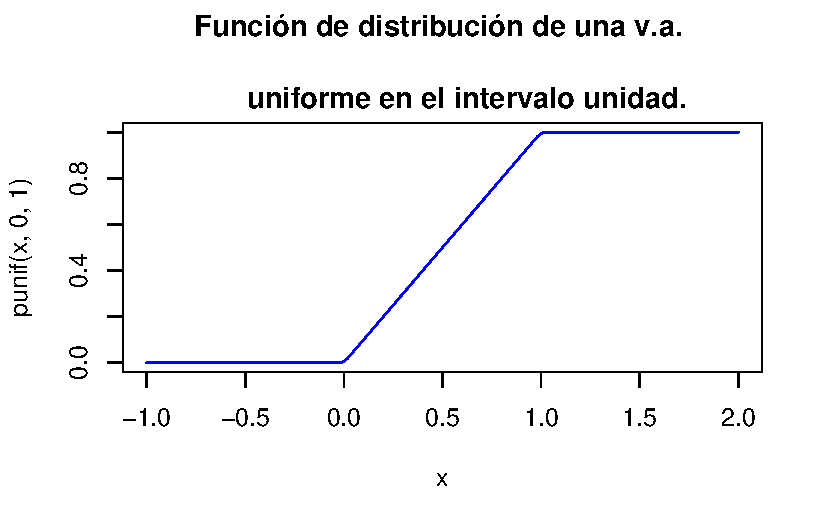
\includegraphics[width=0.45\linewidth,height=\textheight,keepaspectratio]{variables_aleatorias_files/figure-pdf/figUNIF-1.pdf}
\end{center}

Propiedades

En las variables continuas los sucesos del tipo \(\{X\leq x \}\) y
\(\{X< x \}\) tendrán la misma probabilidad. Otras identidades similares
son :

\begin{itemize}
\tightlist
\item
  \(P(X\leq b)=P(X<b)\).
\item
  \(P(X<b)=P(X<a)+P(a<X<b)\).
\item
  \(P(a<X<b)=P(X<b)-P(X<a)\).
\end{itemize}

\textbf{Demostración:}

Algunas identidades son evidentes \(P(X\leq b)=P(X<b)+P(X=b)=P(X<b).\)

Para otras, como la siguiente, podemos hacer

\[\{X\leq a\}\cap \{a<X<b\}=\emptyset\]
\[\{X\leq a\}\cup \{a<X<b\}=\{X<b\},\]

entonces

\(P(X< b)= P(\{X\leq a\}\cup \{a<X<b\}) = P(X\leq a)+P(a<X<b)= P(X< a)+P(a<X<b).\)

La demostración de las otras propiedades las dejamos como ejercicio.

Propiedades de la Función de Distribución

Las propiedades anteriores y combinaciones de ellas se pueden escribir
utilizando la función de distribución de \(X\):

Dada una variable aleatoria continua se tiene que:

\begin{itemize}
\tightlist
\item
  \(F_{X}(b)=F_{X}(a)+P(a<X<b)\).
\item
  \(P(a<X<b)=F_{X}(b)-F_{X}(a)\).
\item
  \(P(a\leq X\leq b)=F_{X}(b)-F_{X}(a)\).
\end{itemize}

Se deja la demostración como ejercicio.

Ejemplo Ejemplo

\textbf{Ejemplo: diana (continuación)}

En el ejemplo de la diana:

\[P(0.25<X<0.3)=F_{X}(0.3)-F_{X}(0.25)=0.3-0.25=0.05.\]

Definición: Función de densidad

Una función \(f:\mathbb{R}\to\mathbb{R}\) es una función de densidad
sobre \(\mathbb{R}\) si cumple que

\begin{itemize}
\tightlist
\item
  \(f_{X}(x)\geq 0\) para todo \(x \in\mathbb{R}.\)
\item
  \(f\) es continua salvo a lo más en una cantidad finita de puntos
  sobre cada intervalo acotado de \(\mathbb{R}\).
\item
  \(\displaystyle\int\limits_{-\infty}^{+\infty} f_{X}(x) dx=1.\)
\end{itemize}

Propiedad: relación entre la función de distribcuión y la densidad

Sea \(X\) una v.a. con función de distribución \(F_X\). Sea
\(f:\mathbb{R}\to\mathbb{R}\) una función de densidad tal que

\[F_X(x)=\displaystyle\int_{-\infty}^{x} f_X(t) dt.\mbox{ para todo } x\in\mathbb{R},\]

Entonces \(X\) es una variable aleatoria continua y \(f_X\) es la
densidad de la v.a. \(X\).

Además el los valores de \(F_X\) son continuos y derivables en los
puntos donde \(f_X\) es continua y la derivada de la función de
distribución es una densidad \(F'_x(x)=f_X(x)\).

Definición: Dominio de una variable aleatoria continua

El conjunto \(D_X=\{x\in\mathbb{R}| f_x(x)>0\}\) recibe el nombre de
soporte o dominio de la variable aleatoria continua y se interpreta como
su conjunto de resultados posibles.

Ejemplo: diana (continuación)

En nuestra ejemplo de la diana, la función \(f\) es una densidad

\[
f_{X}(x)=\left\{
\begin{array}{ll}
0, & \mbox{si } x\leq 0,\\
1, & \mbox{si } 0 < x < 1,\\
0, & \mbox{si } 1\leq x.
\end{array}\right.
\]

que es la densidad de \(X\), en efecto:

\[
f_{X}(x)=\left\{
\begin{array}{ll}
0, & \mbox{si } x\leq 0,\\
1, & \mbox{si } 0 < x < 1,\\
0, & \mbox{si } 1\leq x.
\end{array}\right.
\]

\begin{itemize}
\item
  Si \(x \leq 0\) entonces
  \(\displaystyle\int_{-\infty}^x f_X(t) dt = 0.\)
\item
  Si \(0\leq x\leq 1\) entonces
  \(\displaystyle\int_{-\infty}^x f_X(t) dt = \int_0^x 1 dt = x.\)
\item
  Si \(x\geq 1\) entonces
  \(\displaystyle\int_{-\infty}^x f_X(t) dt = \int_0^1 1 dt = 1.\)
\end{itemize}

Por lo tanto, \(F_X(x)=\displaystyle\int_{-\infty}^x f_X(t) dt\) para
todo \(x\in\mathbb{R}.\)

\begin{Shaded}
\begin{Highlighting}[]
\FunctionTok{curve}\NormalTok{(}\FunctionTok{dunif}\NormalTok{(x,}\DecValTok{0}\NormalTok{,}\DecValTok{1}\NormalTok{),}\AttributeTok{xlim=}\FunctionTok{c}\NormalTok{(}\SpecialCharTok{{-}}\FloatTok{0.5}\NormalTok{,}\FloatTok{1.5}\NormalTok{),}\AttributeTok{col=}\StringTok{"blue"}\NormalTok{,}
      \AttributeTok{main=}\StringTok{"Densidad de la distribución uniforme en [0,1]"}\NormalTok{)}
\end{Highlighting}
\end{Shaded}

\begin{center}
\includegraphics[width=0.5\linewidth,height=\textheight,keepaspectratio]{variables_aleatorias_files/figure-pdf/unnamed-chunk-1-1.pdf}
\end{center}

Propiedades

La función de densidad nos permite calcular diversas probabilidades.

Propiedades de la función de densidad

\begin{itemize}
\item
  Sea \(X\) una v.a. continua con función de distribución \(F_X\) y de
  densidad \(f_X\), entonces \begin{eqnarray*}
  P(a< X< b) &=&  P(a<X\leq b)= P(a\leq X< b)=\\
   & & P(a\leq X\leq b)= \displaystyle\int_{a}^b f_X(x) dx.
  \end{eqnarray*}
\item
  Si \(A\) es un subconjunto adecuado de \(\mathbb{R}\) entonces
  \[P(X\in A)=\displaystyle\int_{A} f(x) dx=\displaystyle\int_{A\cap D_X} f(x) dx.
  \]
\end{itemize}

Propiedades de la función de densidad

Sea \(X\) una v.a. continua con función de distribución \(F_X\) y de
densidad \(f_X\), entonces:

\begin{itemize}
\tightlist
\item
  Si \(f_x\) es continua en un punto \(x\), \(F_X\) es derivable en ese
  punto y \(F_X'(x)=f_X(x).\)
\item
  \(P(X=x)=0\) para todo \(x\in\mathbb{R}.\)
\end{itemize}

Ejercicio

Comprobar estas propiedades en el ejemplo de la diana.

Ejemplo tiempo ejecución de un proceso

Sea \(X=\) tiempo de ejecución de un proceso. Se supone que \(X\) sigue
una distribución uniforme en dos unidades de tiempo, si tarda más el
proceso se cancela.

Calculemos la función de densidad y de distribución de la v.a \(X\).

Entonces

\[
F_{X}(x)=P(X\leq x)=\frac{CF}{CP}=\frac{x}2.
\]

Luego su función de distribución es:

\[
F_{X}(x)=\left\{\begin{array}{ll}
0, & \mbox{si } x\leq 0,\\
\frac{x}2 & \mbox{si } 0<x<2,\\
1, & \mbox{si } 2\leq x.
\end{array}\right.
\]

Su función de densidad por su lado es: \[
f_{X}(x)=F_{X}'(x)=\left\{\begin{array}{ll}
0 & \mbox{si } x\leq 0\\
\frac12 & \mbox{si } 0<x\leq 2\\
0 & \mbox{si } 2\leq x
\end{array}\right.
\]

Efectivamente

\begin{itemize}
\tightlist
\item
  \(f_{X}(x)\geq 0,\) y tiene un conjunto finito de discontinuidades: en
  \(0\) y en \(2\)
\item
  \(F_X(x)=\displaystyle\int_{-\infty}^x f_X(t) dt,\) para todo
  \(x\in \mathbb{R}\) (Ejercicio: resolverlo gráficamente.)
\item
  \(\displaystyle\int_{-\infty}^{+\infty}f_{X}(x)dx=
  \int_0^2\frac12dx=\left[\frac{x}2\right]_0^2
  =\frac22-\frac02=1.\)
\end{itemize}

Ejercicio: Tiempo de un proceso

Calcular la probabilidad de que uno de nuestros procesos tarde más de
una unidad de tiempo en ser procesado. Calcular también la probabilidad
de que dure entre \(0.5\) y \(1.5\) unidades de tiempo.

\section{Esperanza y varianza para variables aleatorias
continuas}\label{esperanza-y-varianza-para-variables-aleatorias-continuas}

Algunas de estas propiedades ya han sido estudiadas en el caso de
variables aleatorias discretas. Por ello, en esta sección nos
centraremos en presentar sus definiciones, métodos de cálculo y algunos
ejemplos en el contexto continuo.

A partir de ahora, salvo indicación en contrario, consideraremos que
\(X\) es una variable aleatoria continua con función de densidad
\(f_{X}(x)\)

Definición: Esperanza y Varianza v.a. continuas

\begin{itemize}
\tightlist
\item
  Su esperanza es:
  \[E(X)=\displaystyle\int\limits_{-\infty}^{+\infty} x\cdot f_{X}(x)dx.\]
\item
  Si \(g(x)\) es una función de la variable \(X\) entonces:
  \[E(g(X))=\displaystyle\int\limits_{-\infty}^{+\infty} g(x)\cdot f_{X}(x)dx.\]
\item
  \textbf{Varianza} \[\sigma_{X}^2=E((X-\mu_{X})^2)=
    \displaystyle\int\limits_{-\infty}^{+\infty} (x-\mu_{X})^2 \cdot f_{X}(x)dx.
    \]
\item
  Su desviación típica es: \[\sigma_{X}=+\sqrt{\sigma_{X}^2}.\]
\end{itemize}

Propiedades

\begin{itemize}
\tightlist
\item
  \(\sigma_{X}^2\geq 0\).
\item
  \(Var(cte)=E(cte^2)-(E(cte))^2= cte^2 - cte^2=0\).
\item
  \(\displaystyle Var(x)=E(X^2)-\mu_{X}^2=\int_{-\infty}^{+\infty}x^2\cdot  f_{X}(x)dx - \mu_{X}^2.\)
\item
  El mínimo de \(E((X-C)^2)\) se alcanza cuando \(C=E(X)\) y es
  \(Var(X)\).
\end{itemize}

Ejemplo: diana (continuación)

\[\mu_{X}=  \int_0^1 x  dx=\left[\frac{x}{2}\right]_0^1=\frac12,\]
\[E(X^2)=\int_0^1 x^2 dx=\left[\frac{x^3}{3}\right]_0^1=\frac13,\]

\[Var(X)=E(X^2)-E(X)^2=\frac13-\left(\frac12\right)^2=\frac1{12}.\]
Podemos comprobar que con la definición directa el resultado es el mismo

\[
Var(X)=E\left(\left(X-E(X)\right)^2\right)=
\int_0^1 \left(x-\frac12\right)^2 dx=
\left[\frac13 \left(x-\frac12\right)^3\right]_0^1= 
\frac13\cdot \left(\left(1-\frac12\right)^3-\left(0-\frac12\right)^3\right)
= \frac13\left(\frac18-\left(-\frac18\right)\right)=\frac13\cdot \frac28=\frac1{12}.
\]

\section{Esperanza de transformaciones lineales de v.a.
continuas}\label{esperanza-de-transformaciones-lineales-de-v.a.-continuas}

Propiedad

Sea \(X\) una v.a. continua con \(E(X)=\mu_{X}\) y
\(Var(X)=\sigma_{X}^2\) sea \(Y=a+b X\), donde \(a,b\in\mathbb{R}\), es
una nueva v.a. continua obtenida mediante una transformación lineal de
\(X\). Se verifican las mismas propiedades que en el caso discreto:

\begin{itemize}
\tightlist
\item
  \(E(Y)=E(a+b\cdot  X)=a+b\cdot  E(X)\).
\item
  \(Var(Y)=Var(a+b\cdot  X)=b^2 \cdot  Var(X)\).
\item
  \(\sigma_{Y}=|b|\cdot  \sigma_{X}\).
\item
  \(Z=\frac{X-\mu_{X}}{\sigma_{X}}\) es una transformación lineal de
  \(X\) de forma que \[E(Z)=0 \mbox{ y } Var(Z)=1\]
\end{itemize}

Ejemplo

En una empresa de venta de vinos por internet, sea \(X=\) número de
litros de vino del país vendidos en un año. Supongamos que sabemos que
\(E(X)=10000\) y que \(Var(X)=100.\) Supongamos que los gastos fijos de
distribución son 50.000 € y el beneficio por litro es de 10 € por
botella. Definimos \(T=10\cdot X-50000,\) que será el beneficio después
de gastos.

Entonces la esperanza del beneficio es \[E(T)=10 E(X)-50000 = 50000,\] y
\[Var(T)=10^2 Var(X)= 10000.\]

\section{Transformaciones de variables
aleatorias}\label{transformaciones-de-variables-aleatorias}

Muchas variables aleatorias son funciones de otras v.a. En lo que sigue
resumiremos diversas técnicas para dada una v.a. \(X\) y una
transformación \(Y=h(X)\) encontrar \(F_{Y}\) a partir de \(F_{X}\).

Propiedad: Transformaciones de v.a. discretas

Sea \(X\) una v.a. discreta con
\(X(\Omega)=\{x_1,x_2,\ldots,x_{n},..\}\) y sea
\(h:\mathbb{R}\to\mathbb{R}\) una aplicación. Entonces \(Y=h(X)\) es
también una v.a. discreta. Además si \(P_X\) y \(F_{X}\) son las
funciones de probabilidad y de distribución de \(X\) entonces

\begin{itemize}
\tightlist
\item
  \(\displaystyle P_{Y}(y)=\sum_{x_{i}|h(x_{i})=y}P_X(x_{i}).\)
\item
  \(\displaystyle F_{Y}(y)=\sum_{x_{i}|h(x_{i})\leq y} P_X(x_{i}).\)
\end{itemize}

Desafortunadamente para variables no discretas el resultado no es tan
sencillo como el anterior, pues la transformación de, por ejemplo, una
v.a. continua puede ser continua, discreta, mixta,\(\ldots\)

Propiedad: Transformación de v.a. continuas en continuas**

Sea \(X\) una v.a. continua cuya función de densidad es \(f_{X}\). Sea
\(h:\mathbb{R}\to\mathbb{R}\), una aplicación estrictamente monótona y
derivable, por lo tanto \(h'(x)\not=0\) para todo \(x\in\mathbb{R}\).
Sea \(Y=h(X)\) la transformación de \(X\) por \(h\). Entonces \(Y\) es
una v.a. continua con función de densidad

\[f_{Y}(y)=\left.\frac{f_{X}(x)}
{\left|h'(x)\right|}\right|_{x=h^{-1}(y)}\]

Densidad de una transformación de una v.a. continua

Sea \(X\) una v.a. continua cuya función de densidad es \(f_{X}\). Sea
\[h:\mathbb{R}\to\mathbb{R}\] una aplicación, no necesariamente monótona
tal que :

\begin{itemize}
\tightlist
\item
  sea derivable con derivada no nula
\item
  la ecuación \(h(x)=y\) tiene un número finito de soluciones
  \(x_1,x_2,..,x_{n}\)
\end{itemize}

entonces:

\[
\displaystyle f_{Y}(y)=\left.\sum_{k=1}^{n} \frac{f_{X}(x)}
{\left|h'(x)\right|}\right|_{x=x_{k}}.
\]

\section{Método general de transformación de
v.a.}\label{muxe9todo-general-de-transformaciuxf3n-de-v.a.}

Cuando no podamos aplicar las propiedades anteriores intentaremos
calcular primero la función de distribución de la transformación y luego
su densidad.

Notemos que en general si \(Y=g(X)\) es una v.a. transformación de la
v.a. \(X\) entonces

\[
F_{Y}(y)=P(Y\leq y)=P(g(X)\leq y).
\]

Por ejemplo, si \(g\) es estrictamente creciente y continua,

\[
F_{Y}(y)=P(g(X)\leq y)=P(X\leq g^{-1}(y))=F_{X}(g^{-1}(y)),
\]

y si \(g\) es estrictamente decreciente y continua, \[
F_{Y}(y)=P(g(X)\leq y)=P(X\geq g^{-1}(y))=1-F_{X}(g^{-1}(y)).
\]

\section{Desigualdades de Markov y de
Chebychev}\label{desigualdades-de-markov-y-de-chebychev}

En esta sección distintas desigualdades que acotan determinadas
probabilidades de una variable aleatoria.

Estas desigualdades sirven en algunos casos para acotar probabilidades
de determinados sucesos.

También son útiles desde el punto de vista teórico, por ejemplo para
justificar que la varianza es una medida de la dispersión de los datos.

\subsection{Desigualdad de Markov}\label{desigualdad-de-markov}

Propiedad: Desigualdad de Markov

Sea \(X\) una v.a. positiva con \(E(X)\) finita. Entonces

\[P(X\geq a)\leq \frac{E(X)}{a}\mbox{ para todo }a>0.\]

\textbf{Demostración}:

Si \(X\) es continua y solo toma valores positivos

\begin{eqnarray*}
E(X) &=& \int_{-\infty}^{+\infty} x\cdot f_{X}(x) dx=  \int_0^{+\infty} x\cdot f_{X}(x) dx=  \int_0^{a} x\cdot f_{X}(x) dx +\int_{a}^{+\infty} x\cdot f_{X}(x) dx \\
& &\geq   \int_{a}^{+\infty} x\cdot
f_{X}(x) dx \geq a \int_{a}^{+\infty}
f_{X}(x) dx = a \cdot  P(X\geq a),
\end{eqnarray*}

de donde se sigue que

\[P(X\geq a)\leq \frac{E(X)}{a}.\]

\subsection{Desigualdad de Markov}\label{desigualdad-de-markov-1}

Sea \(X\) una v.a. con \(E(X)\) finita entonces para todo \(a>0\)

\[P(|X|\geq a )\leq \frac{E(|X|)}{a}.\]

\textbf{Ejercicio}

Demuestra el corolario anterior a partir de la desigualdad de Markov.

\section{Desigualdad de Chebychev}\label{desigualdad-de-chebychev}

Propiedad: Desigualdad de Chebychev

La \textbf{desigualdad de Chebychev} también se denomina de Chebyshov y
en inglés \emph{Chebyshev}.

Desigualdad de Chebychev

Sea \(X\) una v.a.con \(E(X)=\mu\) y \(Var(X)=\sigma^2\) entonces para
todo \(a>0\),

\[P(|X-\mu|\geq a)\leq \frac{\sigma^2}{a^2}.\]

\textbf{Demostración}

Apliquemos la consecuencia de la desigualdad de Markov a la v.a. no
negativa

\[Y^2=(X-\mu)^2\]

entonces

\[
P(Y^2\geq a^2) \leq 
\frac{E(Y^2)}{a^2}=\frac{E((X-\mu)^2)}{a^2}
= \frac{Var(X)}{a^2}=\frac{\sigma^2}{a^2}
.
\]

Por otra parte

\[
P(Y^2\geq a^2)=P(|Y|\geq a)= P(|X-\mu|\geq a),
\]

hecho que, junto con la desigualdad anterior, demuestra el resultado.

\subsection{Uso de la desigualdad de
Chebychev}\label{uso-de-la-desigualdad-de-chebychev}

Utilidad básica de la desigualdad de Chebychev

Supongamos que \(X\) es una v.a. con \(Var(X)=0\), entonces, aplicando
la desigualdad anterior

\[P(|X-E(X)|\geq a )=0\mbox{ para todo }a>0,\]

lo que implica que

\[P(X=E(X))=1,\]

Por lo que la probabilidad de que \(X\) sea constantemente \(E(X)\) es
1, hecho que nos confirma la utilidad de la varianza como una medida de
la dispersión de los datos.

Ejemplo: tiempo de respuesta

Se sabe que el tiempo de respuesta medio y la desviación típica de un
sistema multiusuario son 15 y 3 unidades de tiempo respectivamente.
Entonces:

\[
P(|X-15|\geq 5)\leq \frac9{25}=0.36.
\]

Si substituimos \(a\) por \(a\cdot \sigma\) en la desigualdad de
Chebychev, nos queda:

\[
P(|X-\mu|\geq a\cdot \sigma)\leq
\frac{\sigma^2}{(a\cdot \sigma)^2}=\frac1{a^2},
\]

que es otra manera de expresar la desigualdad de Chebychev.

\section{Más formas de la desgualdad de
Chebychev}\label{muxe1s-formas-de-la-desgualdad-de-chebychev}

La desigualdad de Chebychev también se puede escribir de al menos dos
maneras más:

\[
P(\mu-a\leq X\leq \mu+a)\geq 1-\frac{\sigma^2}{a^2},
\]

y tomado como \(a=k\cdot \sigma\),

\[
P(\mu-k\cdot \sigma\leq X\leq \mu+ k \cdot \sigma)\geq 1-\frac1{k^2}.
\]

\subsection{La varianza como medida de
dispersión}\label{la-varianza-como-medida-de-dispersiuxf3n}

Tomando la segunda expresión que hemos visto para la desigualdad de
Chebychev para distintos valores de \(k>0\) obtenemos la siguiente
tabla:

\begin{table}
\centering
\begin{tabular}{|c|c|}
$k$ &  $P\left(|X-E(X)|\geq k  \cdot \sigma\right)$\\
\hline
$1$ & $\leq 1$ \\
$2$ & $\leq 0.25$ \\
$3$ & $\leq 0.111$ \\
$4$ & $\leq 0.0025$\\ \hline
\end{tabular}
\end{table}

Por ejemplo para \(k=2\), esta desigualdad se puede interpretar como
que, dada una v.a. \(X\) con cualquier distribución que tenga \(E(X)\) y
\(Var(X)\) finitos, \emph{la probabilidad de que un valor se aleje de la
media} \(\mu\) más de \(a=2\) desviaciones típicas es menor o igual que
\(0.25\).

Es decir sólo el 25\% de los valores estarán alejados de la media más de
\(2\cdot \sigma\) ¡\emph{Sea cual sea la distribución de la v.a.}!

\chapter{Distribuciones notables 1}\label{distribuciones-notables-1}

\section{Introducción}\label{introducciuxf3n-1}

En este tema estudiaremos diversos tipos de experimentos que son muy
frecuentes y algunas de las variables aleatorias asociadas a ellos.

Estas variables reciben distintos nombres que aplicaremos sin distinción
al tipo de población del experimento a la variable o a su función de
probabilidad, densidad o distribución.

Empezaremos con las variables aleatorias discretas que se presentan con
frecuencia ya que están relacionadas con situaciones muy comunes como el
número de caras en varios lanzamiento de una moneda, el número de veces
que una maquina funciona hasta que se estropea, el numero de clientes en
una cola,\ldots{}

\section{Distribución Bernoulli}\label{distribuciuxf3n-bernoulli}

Distribución Bernoulli

Consideremos un experimento con dos resultados posibles éxito (E) y
fracaso (F). El espacio de sucesos será \(\Omega=\{E,F\}\).

Supongamos que la probabilidad de éxito es \(P(E)=p\), y naturalmente
\(P(F)=1-p=q\) con \(0<p<1\).

Consideremos la aplicación

\[
X:\Omega=\{E,F\}\to \mathbb{R}
\]

definida por

\[
X(E)=1\mbox{, }X(F)=0.
\]

Su función de probabilidad es

\[
P_{X}(x)=
\left\{
\begin{array}{ll} 1-p=q & \mbox{si } x=0\\
p & \mbox{si } x=1\\
0 & \mbox{en cualquier otro caso}
\end{array}
\right..
\]

Su función de distribución es

\[
F_{X}(x)=P(X\leq x)=
\left\{
\begin{array}{ll} 
0 & \mbox{si } x<0\\
1-p=q & \mbox{si } 0\leq x <1\\
1 & \mbox{si } 1\leq x \\
\end{array}
\right..
\]

Bajo estas condiciones diremos que \(X\) \textbf{es una v.a. Bernoulli}
o que sigue una ley de \textbf{distribución de probabilidad Bernoulli}
de parámetro \(p\). * Lo denotaremos por
\[X\sim Ber(p)\mbox{ o también } X\sim B(1,p).\]

Este tipo de experimentos (éxito/fracaso)se reciben el nombre de
experimentos Bernoulli.

Fue su descubridor un científico suizo
\href{https://es.wikipedia.org/wiki/Jakob_Bernoulli}{Jacob Bernoulli},
uno más de la conocida
\href{https://es.wikipedia.org/wiki/Familia_Bernoulli}{familia de
científicos suizos Bernoulli}.

Su \textbf{valor esperado} es

\[E(X)=\displaystyle\sum_{x=0}^1 x\cdot P(X=x)= 0\cdot(1-p)+1\cdot p=p.\]

Calculemos también \(E(X^2)\)

\[E(X^2)=\displaystyle\sum_{x=0}^1 x^2\cdot P(X=x)= 0^2\cdot(1-p)+1^2\cdot p=p.\]

La \textbf{varianza} de una va.a Bernouilli es

\[Var(X)=E(X^2)-\left(E(X)\right)^2=p-p^2=p\cdot (1-p)=p\cdot q.\]

Su desviación típica es

\[
\sqrt{Var(X)}=\sqrt{p \cdot (1-p)}.
\]

Pongamos en una tabla resumen v.a con distribución Bernoulli

\renewcommand{\arraystretch}{1.75}
\begin{table}
\centering
\begin{tabular}{|l|}
\hline\rowcolor{LightBlue}
$X$ Bernoulli:  $Ber(p)$ 
\\\hline
$\scriptstyle{ D_X=   \{0,1\}}$  
\\\hline
$\scriptsize{P_X(x)=P(X=x)=
\left\{
\begin{array}{ll}
1-p=q & \mbox{ si } x=0\\
p & \mbox{ si } x=1 \\
0  & \mbox{ en otro caso.}
\end{array}\right.}
$ 
\\\hline
$\scriptsize{  F_X(x)=P(X\leq X)=
\left\{
\begin{array}{ll}
  0 &   \mbox{ si } x<0\\ 
 (1-p)  &  \mbox{ si } 0\leq x< 1 \\ 
1 & \mbox{ si } x\geq 1
\end{array}
\right.}$.
\\\hline
$\scriptstyle E(X)=p$; $\scriptstyle  Var(X)= p \cdot (1-p)$ \\\hline
\end{tabular}
\end{table}

Ejemplo : Cálculos con R

Veamos los cálculos básicos \(Ber(p=0.25)\) en \texttt{R}.

\begin{Shaded}
\begin{Highlighting}[]
\FunctionTok{dbinom}\NormalTok{(}\DecValTok{0}\NormalTok{,}\AttributeTok{size=}\DecValTok{1}\NormalTok{,}\AttributeTok{prob=}\FloatTok{0.25}\NormalTok{)}
\end{Highlighting}
\end{Shaded}

\begin{verbatim}
[1] 0.75
\end{verbatim}

\begin{Shaded}
\begin{Highlighting}[]
\FunctionTok{dbinom}\NormalTok{(}\DecValTok{1}\NormalTok{,}\AttributeTok{size=}\DecValTok{1}\NormalTok{,}\AttributeTok{prob=}\FloatTok{0.25}\NormalTok{)}
\end{Highlighting}
\end{Shaded}

\begin{verbatim}
[1] 0.25
\end{verbatim}

\begin{Shaded}
\begin{Highlighting}[]
\FunctionTok{rbinom}\NormalTok{(}\AttributeTok{n=}\DecValTok{20}\NormalTok{,}\AttributeTok{size =} \DecValTok{1}\NormalTok{,}\AttributeTok{prob=}\FloatTok{0.25}\NormalTok{)}
\end{Highlighting}
\end{Shaded}

\begin{verbatim}
 [1] 0 0 0 0 0 0 0 1 1 0 1 0 0 0 1 0 0 0 0 0
\end{verbatim}

El siguiente código dibuja las función de probabilidad y la de
distribución de una \(Ber(p=0.25)\)

\begin{center}
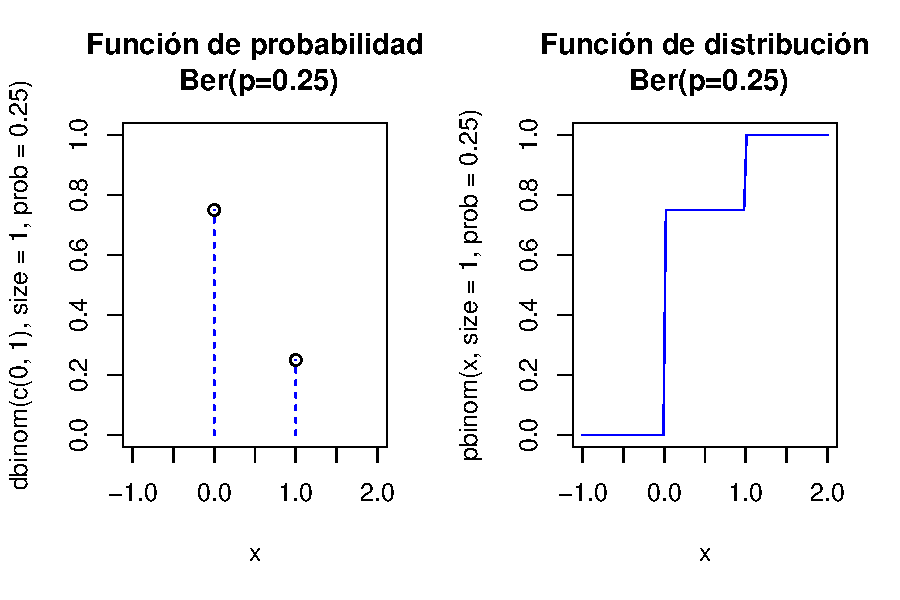
\includegraphics[width=0.7\linewidth,height=\textheight,keepaspectratio]{distibuciones_notables_1_files/figure-pdf/ber_plot_1-1.pdf}
\end{center}

\section{Distribución binomial}\label{distribuciuxf3n-binomial}

Distribución binomial

Si repetimos \(n\) veces de forma independiente un experimento Bernoulli
de parámetro \(p\).

El espacio muestral \(\Omega\) estará formado por cadenas de \(E\)'s y
\(F\)'s de longitud \(n\) Consideremos la v.a.

\[X(\overbrace{EFFF\ldots EEF}^{n})=\mbox{número de éxitos en la cadena}.\]
A la variable aleatoria anterior se le conoce como distribución binomial
de parámetros \(n\) y \(p\), y lo denotaremos por \(X\sim B(n,p).\)

Obviamente se tiene que una v.a. Bernoulli es una binomial con \(n=1\)

\[B(1,p)=Ber(p).\]

La \textbf{función de probabilidad} de una binomial es

\[
P_{X}(x)=\left\{
\begin{array}{ll}
{n\choose x}\cdot  p^x \cdot(1-p)^{n-x} &\mbox{ si } x=0,1,\ldots,n\\
0  & \mbox{ en otro caso}
\end{array}\right..
\]

Su \textbf{función de distribución} no tiene una fórmula cerrada. Hay
que acumular la función de probabilidad:

\begin{eqnarray*}
F_{X}(x)=P(X\leq x) & = & \sum_{i=0}^x P_X(i)\\
& = & 
\left\{
\begin{array}{ll}
0 & \mbox{ si } x<0\\\displaystyle
\sum_{i=0}^k {n\choose i}\cdot  p^i \cdot (1-p)^{n-i} & \mbox{ si } 
\left\{
  \begin{array}{l} 
  k\leq x< k+1\\
  k=0,1,\ldots,n.
  \end{array}
\right.\\
1 & \mbox{ si } n\leq x
\end{array}
\right.
\end{eqnarray*}

Recordemos los números binomiales con un ejemplo

Números binomiales

Los números binomiales calculan el número de equipos de baloncesto
distintos que (\(k=5\) jugadores) se pueden hacer con 6 jugadores
(\(n=6\)).

Es decir cuántas maneras distintas hay para elegir (\emph{choose}) 5
jugadores en un conjunto de 6 jugadores. Todo el mundo diría ¡¡¡6!!!.
Efectivamente con R es

\begin{Shaded}
\begin{Highlighting}[]
\FunctionTok{choose}\NormalTok{(}\DecValTok{6}\NormalTok{,}\DecValTok{5}\NormalTok{)}
\end{Highlighting}
\end{Shaded}

\begin{verbatim}
[1] 6
\end{verbatim}

Con 10 jugadores el número de equipos de 5 distintos es bastante más
grande

\begin{Shaded}
\begin{Highlighting}[]
\FunctionTok{choose}\NormalTok{(}\DecValTok{10}\NormalTok{,}\DecValTok{5}\NormalTok{)}
\end{Highlighting}
\end{Shaded}

\begin{verbatim}
[1] 252
\end{verbatim}

Y, por ejemplo, con un equipo de fútbol profesional que tiene en
plantilla 22 jugadores (quitando los guardametas) se pueden formar
¡¡nada menos que!!

\begin{Shaded}
\begin{Highlighting}[]
\FunctionTok{choose}\NormalTok{(}\DecValTok{22}\NormalTok{,}\DecValTok{10}\NormalTok{)}
\end{Highlighting}
\end{Shaded}

\begin{verbatim}
[1] 646646
\end{verbatim}

un bonito número capicúa que nos da el número de equipos distintos que
se pueden formar.

Ejercicio

Calculad las funciones de distribución de una binomial \(B(n=1,p=0.3)\)
y comprobar que coinciden con las distribuciones de una \(Ber(p=0.3)\).

Observaciones sobre la distribución binomial

\begin{itemize}
\tightlist
\item
  La probabilidad de fracaso se suele denotar con \(q=1-p\), \textbf{sin
  ningún aviso adicional}, con el fin de acortar y agilizar la escritura
  de las fórmulas.
\item
  Su \textbf{función de distribución no tienen una formula general}, hay
  que calcularla con una función de R o python\ldots{} En el siglo
  pasado se tabulaban en los libros de papel :-).
\item
  En el material adicional os pondremos unas tablas de esta distribución
  para distintos valores de \(n\) y \(p\) para que disfrutéis de tan
  ancestral método de cálculo.
\item
  Cualquier paquete estadístico, hoja de cálculo dispone de funciones
  para el cálculo de estas probabilidades, así que el \textbf{uso de las
  tablas} queda \textbf{totalmente anticuado}.
\end{itemize}

La \textbf{esperanza} de una v.a. \(X\) con distribución \(B(n,p)\) es

\[E(X)=\displaystyle\sum_{k=0}^n k \cdot  {n \choose k }\cdot p^k\cdot q^{n-k} = n\cdot p.\]

La esperanza de \(X^2\) es

\begin{eqnarray*}
E(X^2)&=& \displaystyle\sum_{k=0}^n k^2 \cdot  {n \choose k }\cdot p^k\cdot q^{n-k}\\
&=& n\cdot p\cdot q+(n\cdot p)^2.
\end{eqnarray*}

Por lo tanto su \textbf{varianza} se calcula así

\[Var(X)=E(X^2)-\left(E(X)\right)^2=n\cdot p \cdot q=n\cdot p\cdot (1-p).\]

Su desviación típica es

\[\sqrt{n\cdot p\cdot q}=\sqrt{n\cdot p\cdot (1-p)}.\]

En temas posteriores veremos una forma sencilla del cálculo de la
esperanza y varianza de una \(B(n,p)\) como las suma de \(n\) v.a.
\(Ber(p)\) independientes.

Ejercicio

Justificar de forma intuitiva que si \(X_i\) con \(i=1,2,\ldots, n\) son
v.a. \(Ber(p)\) independientes entonces
\(X=\displaystyle\sum_{i=1}^n X_i\) sigue una distribución \(B(n,p).\)

\subsection{\texorpdfstring{Resumen v.a con distribución binomial
\(B(n,p)\)}{Resumen v.a con distribución binomial B(n,p)}}\label{resumen-v.a-con-distribuciuxf3n-binomial-bnp}

\renewcommand{\arraystretch}{1.75}
\begin{table}
\centering
\begin{tabular}{|l|}
\hline\rowcolor{LightBlue}
$X$ binomial:   $B(n,p)$ \\\hline
$\scriptstyle  D_X=   \{0,1,\ldots n\}$  \\\hline
$\scriptstyle P_X(x)=P(X=x)=\left\{\begin{array}{ll}\scriptstyle {n\choose x}\cdot  p^x\cdot  (1-p)^{n-x} & \mbox{ si } x=0,1,\ldots,n\\0  & \mbox{ en otro caso.}\end{array}\right.$ \\\hline
$\scriptstyle  F_X(x)=P(X\leq X)=
\scriptstyle\left\{
\begin{array}{ll}
\scriptstyle  0 & \scriptstyle  \mbox{ si } x<0\\ 
\scriptstyle \sum_{i=0}^k {n\choose i}\cdot  p^i\cdot  (1-p)^{n-i} &  
\scriptstyle \mbox{si } \scriptstyle k\leq x< k+1 \mbox{\small para } \scriptstyle k=0,1,\dots,n \\ 
\scriptstyle 1 & \scriptstyle  \mbox{ si } x\geq n
\end{array}
\right.$.\\\hline
$\scriptstyle E(X)=n\cdot p$; $\scriptstyle  Var(X)=n\cdot p \cdot (1-p)$ \\\hline
\end{tabular}
\end{table}

\subsection{Cálculos binomial con R}\label{cuxe1lculos-binomial-con-r}

Veamos los cálculos básicos con funciones de R para una v.a \(X\) con
distribución binomial \(B(n=10,p=0.25)\).

Si queremos calcular con \texttt{R} algún valor de la función de
distribución como por ejemplo \(F_X(0)=P(X\leq 0)\), tenemos que hacer:

\begin{Shaded}
\begin{Highlighting}[]
\FunctionTok{pbinom}\NormalTok{(}\DecValTok{0}\NormalTok{,}\AttributeTok{size=}\DecValTok{10}\NormalTok{,}\AttributeTok{prob=}\FloatTok{0.25}\NormalTok{)}
\end{Highlighting}
\end{Shaded}

\begin{verbatim}
[1] 0.05631351
\end{verbatim}

y si queremos por ejemplo \(F_X(4)=P(X\leq 4)\), tenemos que hacer:

\begin{Shaded}
\begin{Highlighting}[]
\FunctionTok{pbinom}\NormalTok{(}\DecValTok{4}\NormalTok{,}\AttributeTok{size=}\DecValTok{10}\NormalTok{,}\AttributeTok{prob=}\FloatTok{0.25}\NormalTok{)}
\end{Highlighting}
\end{Shaded}

\begin{verbatim}
[1] 0.9218731
\end{verbatim}

Sin embargo, si queremos calcular algún valor de la función de
probabilidad como por ejemplo \(P(X=0)\), tenemos que hacer:

\begin{Shaded}
\begin{Highlighting}[]
\FunctionTok{dbinom}\NormalTok{(}\DecValTok{0}\NormalTok{,}\AttributeTok{size=}\DecValTok{10}\NormalTok{,}\AttributeTok{prob=}\FloatTok{0.25}\NormalTok{)}
\end{Highlighting}
\end{Shaded}

\begin{verbatim}
[1] 0.05631351
\end{verbatim}

o por ejemplo para \(P(X=4)\):

\begin{Shaded}
\begin{Highlighting}[]
\FunctionTok{dbinom}\NormalTok{(}\DecValTok{4}\NormalTok{,}\AttributeTok{size=}\DecValTok{10}\NormalTok{,}\AttributeTok{prob=}\FloatTok{0.25}\NormalTok{)}
\end{Highlighting}
\end{Shaded}

\begin{verbatim}
[1] 0.145998
\end{verbatim}

\subsubsection{Generación de muestras aleatorias con
R}\label{generaciuxf3n-de-muestras-aleatorias-con-r}

Generaremos una muestra aleatoria de 100 valores de una población con
distribución \(B(20,0.5)\)

\begin{Shaded}
\begin{Highlighting}[]
\FunctionTok{set.seed}\NormalTok{(}\DecValTok{2019}\NormalTok{)}
\FunctionTok{rbinom}\NormalTok{(}\DecValTok{100}\NormalTok{,}\AttributeTok{size =} \DecValTok{20}\NormalTok{,}\AttributeTok{prob=}\FloatTok{0.5}\NormalTok{)}
\end{Highlighting}
\end{Shaded}

\begin{verbatim}
  [1] 12 11  9 11  6  6 12  5  7 11 12 11  8  8 11 11  7 11  9 10  9 10 14
 [24]  8  8  5 11 14 11 10 11  5 12  8  6  7  9 10  5 12 11  9 12 11 12 10
 [47] 13 13  8  8  9  7  6  9 10  9 16 13  6  6  8  8 11  9 12 15  9  7 12
 [70] 11  9  8  9  8 11 15  7 10  9 12  6 13 14  8 10  8 10 11 11  9 10 11
 [93] 12  8 10 12  9 13  9 13
\end{verbatim}

Que corresponde a los resultados de repetir 100 veces el experimento de
lanzar una moneda 20 veces y contar el número de caras.

\subsection{Cálculos distribución binomial con
python}\label{cuxe1lculos-distribuciuxf3n-binomial-con-python}

Veamos los cálculos básicos con funciones de python para una v.a \(X\)
con distribución binomial \(B(n=10,p=0.25)\).

Primero importamos la función \texttt{binom} de la librería
\texttt{scipy.stat}

\begin{Shaded}
\begin{Highlighting}[]
\ImportTok{from}\NormalTok{ scipy.stats }\ImportTok{import}\NormalTok{ binom}
\end{Highlighting}
\end{Shaded}

En general en el paquete \texttt{scipy}, la función de probabilidad se
invocará con el método \texttt{pmf}, la de distribución con el método
\texttt{cdf} mientras que una muestra aleatoria que siga esta
distribución con el método \texttt{rvs}. En todos ellos aparecerá
siempre el parámetro \texttt{loc} que se utiliza para desplazar el
dominio de la variable aleatoria. Por ejemplo, en este caso

\begin{Shaded}
\begin{Highlighting}[]
\NormalTok{binom.pmf(k, n, p, loc) }\OperatorTok{=}\NormalTok{  binom.pmf(k }\OperatorTok{{-}}\NormalTok{ loc, n, p)}
\end{Highlighting}
\end{Shaded}

Para calcular los valores de la función de distribución como por ejemplo
\(F_X(0)=P(X\leq 0)\) y \(F_X(4)=P(X\leq 4)\) utilizamos la función
\texttt{cdf}

\begin{Shaded}
\begin{Highlighting}[]
\NormalTok{binom.cdf(}\DecValTok{0}\NormalTok{,n}\OperatorTok{=}\DecValTok{10}\NormalTok{,p}\OperatorTok{=}\FloatTok{0.25}\NormalTok{)}
\end{Highlighting}
\end{Shaded}

\begin{verbatim}
0.056313514709472684
\end{verbatim}

\begin{Shaded}
\begin{Highlighting}[]
\NormalTok{binom.cdf(}\DecValTok{4}\NormalTok{,n}\OperatorTok{=}\DecValTok{10}\NormalTok{,p}\OperatorTok{=}\FloatTok{0.25}\NormalTok{)}
\end{Highlighting}
\end{Shaded}

\begin{verbatim}
0.9218730926513672
\end{verbatim}

Notemos que al no indicar el valor de \texttt{loc}, se le asume que toma
el valor 0.

\section{Cálculos distribución binomial con
python}\label{cuxe1lculos-distribuciuxf3n-binomial-con-python-1}

Para calcular los valores de la función de probabilidad \(P(X=0)\) y
\(P(X=4)\) utilizamos la función \texttt{pmf}:

\begin{Shaded}
\begin{Highlighting}[]
\NormalTok{binom.pmf(}\DecValTok{0}\NormalTok{,n}\OperatorTok{=}\DecValTok{10}\NormalTok{,p}\OperatorTok{=}\FloatTok{0.25}\NormalTok{)}
\end{Highlighting}
\end{Shaded}

\begin{verbatim}
0.056313514709472656
\end{verbatim}

\begin{Shaded}
\begin{Highlighting}[]
\NormalTok{binom.pmf(}\DecValTok{4}\NormalTok{,n}\OperatorTok{=}\DecValTok{10}\NormalTok{,p}\OperatorTok{=}\FloatTok{0.25}\NormalTok{)}
\end{Highlighting}
\end{Shaded}

\begin{verbatim}
0.14599800109863284
\end{verbatim}

Notemos que al no indicar el valor de \texttt{loc}, se le asume que toma
el valor 0.

Si queremos generar una muestras aleatorias que siga una distribución
binomial, podemos usar la función \texttt{rvs}. En este caso,
generaremos una muestra aleatoria de 100 valores de una población
\(B(20,0.5)\)

\begin{Shaded}
\begin{Highlighting}[]
\NormalTok{binom.rvs(n}\OperatorTok{=}\DecValTok{20}\NormalTok{,p}\OperatorTok{=}\FloatTok{0.25}\NormalTok{,size }\OperatorTok{=} \DecValTok{100}\NormalTok{)}
\end{Highlighting}
\end{Shaded}

\begin{verbatim}
array([3, 5, 9, 2, 9, 6, 1, 7, 6, 3, 7, 6, 5, 8, 4, 5, 1, 6, 5, 7, 4, 6,
       7, 4, 7, 4, 6, 5, 4, 7, 6, 2, 5, 9, 5, 8, 8, 5, 5, 4, 4, 6, 6, 5,
       7, 6, 7, 7, 3, 7, 4, 5, 5, 9, 3, 4, 5, 7, 5, 7, 4, 5, 5, 8, 5, 5,
       3, 5, 5, 3, 5, 2, 5, 6, 5, 4, 3, 5, 8, 3, 4, 6, 6, 2, 2, 6, 5, 2,
       7, 4, 3, 4, 3, 5, 7, 2, 5, 6, 3, 1], dtype=int64)
\end{verbatim}

Observación

Notemos que la secuencia aleatoria generada no es la misma que con
\texttt{R}. De hecho, si volvemos a ejecutar esta función obtendremos
una muestra aleatoria distinta.

\begin{Shaded}
\begin{Highlighting}[]
\NormalTok{binom.rvs(n}\OperatorTok{=}\DecValTok{20}\NormalTok{,p}\OperatorTok{=}\FloatTok{0.25}\NormalTok{,size }\OperatorTok{=} \DecValTok{100}\NormalTok{)}
\end{Highlighting}
\end{Shaded}

\begin{verbatim}
array([ 3,  3,  7,  6,  5,  9,  6,  5,  6,  6,  4,  7,  4,  2,  3,  4,  8,
        4,  6,  4,  2,  7,  4,  1,  3,  3,  5,  4,  6,  8,  6,  5,  5,  5,
        3,  1,  4,  2,  4,  3,  6,  3,  7,  7, 10,  4,  4,  4,  3,  3,  6,
        4,  7,  2,  4,  5,  7,  5,  5,  3,  5,  4,  4,  7,  7,  8,  3,  2,
        4,  5,  3,  4,  2,  8,  4,  3,  3,  6,  8,  4,  5,  5,  4,  8,  4,
        6,  6,  5,  8,  5,  8,  3,  4,  5,  1, 10,  6,  4,  6,  4],
      dtype=int64)
\end{verbatim}

\subsection{Cálculos binomial con
python}\label{cuxe1lculos-binomial-con-python}

Veamos algunos cálculos básicos con funciones de python para la binomial
\(B(n=10,p=0.25)\).

\begin{Shaded}
\begin{Highlighting}[]
\NormalTok{binom.cdf(}\DecValTok{5}\NormalTok{,n}\OperatorTok{=}\DecValTok{10}\NormalTok{,p}\OperatorTok{=}\FloatTok{0.25}\NormalTok{)}
\end{Highlighting}
\end{Shaded}

\begin{verbatim}
0.9802722930908203
\end{verbatim}

\begin{Shaded}
\begin{Highlighting}[]
\NormalTok{binom.pmf(}\DecValTok{1}\NormalTok{,n}\OperatorTok{=}\DecValTok{10}\NormalTok{,p}\OperatorTok{=}\FloatTok{0.25}\NormalTok{)}
\end{Highlighting}
\end{Shaded}

\begin{verbatim}
0.1877117156982421
\end{verbatim}

\begin{Shaded}
\begin{Highlighting}[]
\NormalTok{binom.rvs(n}\OperatorTok{=}\DecValTok{20}\NormalTok{,p}\OperatorTok{=}\FloatTok{0.25}\NormalTok{,size}\OperatorTok{=}\DecValTok{10}\NormalTok{)}
\end{Highlighting}
\end{Shaded}

\begin{verbatim}
array([10,  5,  7,  8,  5,  5,  6,  2,  3,  5], dtype=int64)
\end{verbatim}

\subsection{Gráficas de la distribución binomial con
R}\label{gruxe1ficas-de-la-distribuciuxf3n-binomial-con-r}

El siguiente código de R dibuja las función de probabilidad y la de
distribución de una \(B(n=10,p=0.25)\)

\begin{center}
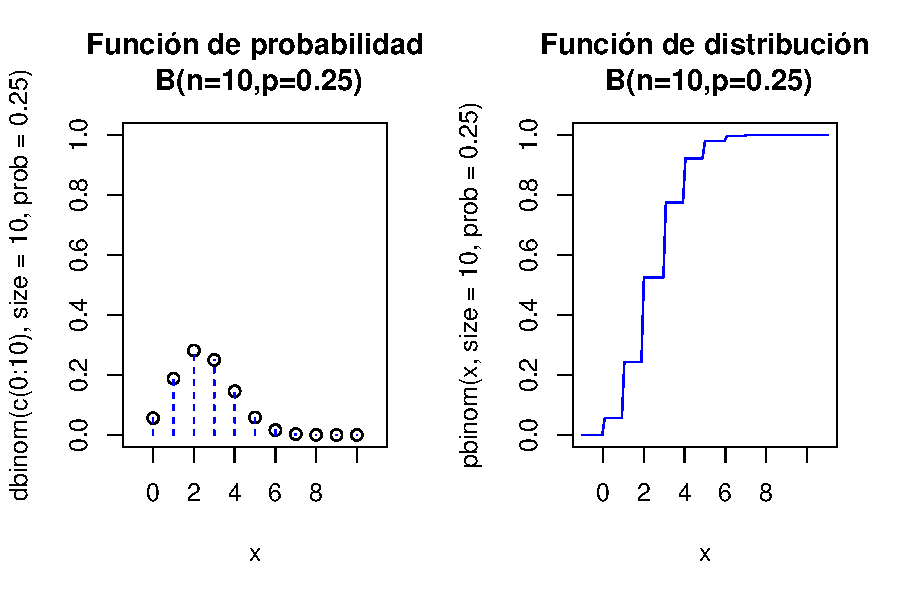
\includegraphics[width=0.55\linewidth,height=\textheight,keepaspectratio]{distibuciones_notables_1_files/figure-pdf/unnamed-chunk-7-1.pdf}
\end{center}

\subsection{Gráficos de la distribución binomial con
python}\label{gruxe1ficos-de-la-distribuciuxf3n-binomial-con-python}

Necesitaremos usar estas librerías:

\begin{Shaded}
\begin{Highlighting}[]
\ImportTok{import}\NormalTok{ numpy }\ImportTok{as}\NormalTok{ np}
\ImportTok{import}\NormalTok{ matplotlib.pyplot }\ImportTok{as}\NormalTok{ plt}
\ImportTok{import}\NormalTok{ scipy.stats }\ImportTok{as}\NormalTok{ stats}
\end{Highlighting}
\end{Shaded}

\begin{Shaded}
\begin{Highlighting}[]
\CommentTok{\# Parámetros de la distribución binomial}
\NormalTok{n }\OperatorTok{=} \DecValTok{10}
\NormalTok{p }\OperatorTok{=} \FloatTok{0.7}

\CommentTok{\# Valores posibles de X}
\NormalTok{x }\OperatorTok{=}\NormalTok{ np.arange(}\DecValTok{0}\NormalTok{, n}\OperatorTok{+}\DecValTok{1}\NormalTok{)}

\CommentTok{\# Función de probabilidad (PMF)}
\NormalTok{pmf\_values }\OperatorTok{=}\NormalTok{ stats.binom.pmf(x, n, p)}

\CommentTok{\# Función de distribución acumulada (CDF)}
\NormalTok{cdf\_values }\OperatorTok{=}\NormalTok{ stats.binom.cdf(x, n, p)}

\CommentTok{\# Graficar la función de probabilidad (PMF)}
\NormalTok{plt.figure(figsize}\OperatorTok{=}\NormalTok{(}\DecValTok{12}\NormalTok{, }\DecValTok{5}\NormalTok{))}
\NormalTok{plt.subplot(}\DecValTok{1}\NormalTok{, }\DecValTok{2}\NormalTok{, }\DecValTok{1}\NormalTok{)}
\NormalTok{plt.bar(x, pmf\_values, color}\OperatorTok{=}\StringTok{\textquotesingle{}blue\textquotesingle{}}\NormalTok{, alpha}\OperatorTok{=}\FloatTok{0.7}\NormalTok{, label}\OperatorTok{=}\StringTok{\textquotesingle{}P(X=k)\textquotesingle{}}\NormalTok{)}
\NormalTok{plt.xlabel(}\StringTok{\textquotesingle{}Valores de X\textquotesingle{}}\NormalTok{)}
\NormalTok{plt.ylabel(}\StringTok{\textquotesingle{}Probabilidad\textquotesingle{}}\NormalTok{)}
\NormalTok{plt.title(}\StringTok{\textquotesingle{}Función de Probabilidad (PMF) {-} Binomial(10, 0.7)\textquotesingle{}}\NormalTok{)}
\NormalTok{plt.xticks(x)}
\end{Highlighting}
\end{Shaded}

\begin{verbatim}
([<matplotlib.axis.XTick object at 0x000001BE393DFFD0>, <matplotlib.axis.XTick object at 0x000001BE393DF670>, <matplotlib.axis.XTick object at 0x000001BE393D1AF0>, <matplotlib.axis.XTick object at 0x000001BE39D27F10>, <matplotlib.axis.XTick object at 0x000001BE39D21D90>, <matplotlib.axis.XTick object at 0x000001BE39D21670>, <matplotlib.axis.XTick object at 0x000001BE39D1C5B0>, <matplotlib.axis.XTick object at 0x000001BE39D216D0>, <matplotlib.axis.XTick object at 0x000001BE39D27220>, <matplotlib.axis.XTick object at 0x000001BE39D1CD90>, <matplotlib.axis.XTick object at 0x000001BE39D2CB80>], [Text(0, 0, ''), Text(0, 0, ''), Text(0, 0, ''), Text(0, 0, ''), Text(0, 0, ''), Text(0, 0, ''), Text(0, 0, ''), Text(0, 0, ''), Text(0, 0, ''), Text(0, 0, ''), Text(0, 0, '')])
\end{verbatim}

\begin{Shaded}
\begin{Highlighting}[]
\NormalTok{plt.legend()}
\NormalTok{plt.grid(axis}\OperatorTok{=}\StringTok{\textquotesingle{}y\textquotesingle{}}\NormalTok{, linestyle}\OperatorTok{=}\StringTok{\textquotesingle{}{-}{-}\textquotesingle{}}\NormalTok{, alpha}\OperatorTok{=}\FloatTok{0.7}\NormalTok{)}

\CommentTok{\# Graficar la función de distribución acumulada (CDF)}
\NormalTok{plt.subplot(}\DecValTok{1}\NormalTok{, }\DecValTok{2}\NormalTok{, }\DecValTok{2}\NormalTok{)}
\NormalTok{plt.step(x, cdf\_values, where}\OperatorTok{=}\StringTok{\textquotesingle{}mid\textquotesingle{}}\NormalTok{, color}\OperatorTok{=}\StringTok{\textquotesingle{}red\textquotesingle{}}\NormalTok{, label}\OperatorTok{=}\StringTok{\textquotesingle{}F(X)\textquotesingle{}}\NormalTok{)}
\NormalTok{plt.scatter(x, cdf\_values, color}\OperatorTok{=}\StringTok{\textquotesingle{}red\textquotesingle{}}\NormalTok{)}
\NormalTok{plt.xlabel(}\StringTok{\textquotesingle{}Valores de X\textquotesingle{}}\NormalTok{)}
\NormalTok{plt.ylabel(}\StringTok{\textquotesingle{}Probabilidad acumulada\textquotesingle{}}\NormalTok{)}
\NormalTok{plt.title(}\StringTok{\textquotesingle{}Función de Distribución Acumulada (CDF) {-} Binomial(10, 0.7)\textquotesingle{}}\NormalTok{)}
\NormalTok{plt.xticks(x)}
\end{Highlighting}
\end{Shaded}

\begin{verbatim}
([<matplotlib.axis.XTick object at 0x000001BE39D2CEE0>, <matplotlib.axis.XTick object at 0x000001BE39D2C940>, <matplotlib.axis.XTick object at 0x000001BE39D501F0>, <matplotlib.axis.XTick object at 0x000001BE39D901F0>, <matplotlib.axis.XTick object at 0x000001BE39D9D4C0>, <matplotlib.axis.XTick object at 0x000001BE39D943D0>, <matplotlib.axis.XTick object at 0x000001BE39D94C10>, <matplotlib.axis.XTick object at 0x000001BE39D7C3A0>, <matplotlib.axis.XTick object at 0x000001BE39D81EE0>, <matplotlib.axis.XTick object at 0x000001BE39D90DF0>, <matplotlib.axis.XTick object at 0x000001BE39D9D520>], [Text(0, 0, ''), Text(0, 0, ''), Text(0, 0, ''), Text(0, 0, ''), Text(0, 0, ''), Text(0, 0, ''), Text(0, 0, ''), Text(0, 0, ''), Text(0, 0, ''), Text(0, 0, ''), Text(0, 0, '')])
\end{verbatim}

\begin{Shaded}
\begin{Highlighting}[]
\NormalTok{plt.legend()}
\NormalTok{plt.grid(axis}\OperatorTok{=}\StringTok{\textquotesingle{}y\textquotesingle{}}\NormalTok{, linestyle}\OperatorTok{=}\StringTok{\textquotesingle{}{-}{-}\textquotesingle{}}\NormalTok{, alpha}\OperatorTok{=}\FloatTok{0.7}\NormalTok{)}

\CommentTok{\# Mostrar gráficos}
\NormalTok{plt.tight\_layout()}
\NormalTok{plt.show()}
\end{Highlighting}
\end{Shaded}

\begin{center}
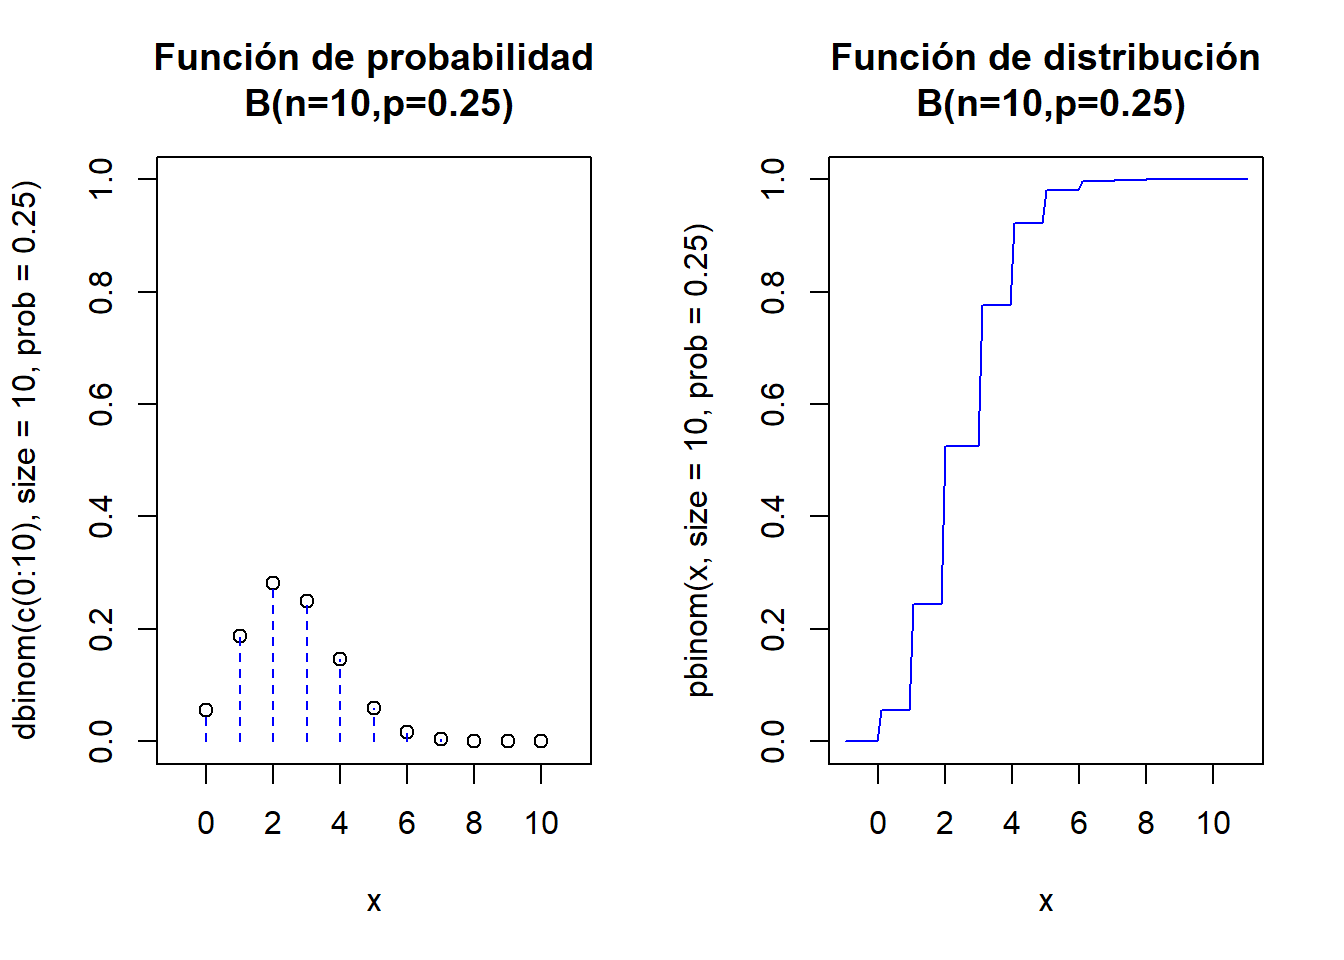
\includegraphics[width=0.7\linewidth,height=\textheight,keepaspectratio]{distibuciones_notables_1_files/figure-pdf/unnamed-chunk-9-1.pdf}
\end{center}

Ejemplo: número de bolas rojas extraídas de una urna con reposición

Tenemos una urna con \(100\) bolas de las cuales 40 son rojas y 60 son
blancas. Extraemos al azar una bola, anotamos su color y la devolvemos a
(reponemos en) la urna.

Supongamos que repetimos este proceso \(n=10\) reponiendo en cada
ocasión la bola extraída.

Consideremos la variable aleatoria \(X\) como el número de bolas rojas
extraídas (con reposición) en \(n=10\) repeticiones del mismo
experimento de Bernoulli.

Bajo estas condiciones repetimos \(n=10\) veces el mismo experimento de
Bernoulli con probabilidad de éxito (sacar bola roja)
\[P(Roja)=P(Éxito)=p=\frac{40}{100}=0.4.\]

Así que la variable \(X\) que es el número de bolas rojas extraídas de
la urna (con reposición) en \(n=10\) ocasiones sigue una ley binomial
\(B(n=10,p=0.4).\)

Nos preguntamos:

\begin{enumerate}
\def\labelenumi{\arabic{enumi}.}
\tightlist
\item
  ¿Cuál es la probabilidad de que saquemos exactamente \(4\) bolas
  rojas?
\item
  ¿Cuál es la probabilidad de que saquemos al menos \(4\) bolas rojas?
\item
  ¿Cuál es la probabilidad de que saquemos menos de \(3\) bolas rojas?
\item
  ¿Cuál es el valor esperado del número de bolas rojas?
\item
  ¿Cuál es la desviación típica del número de bolas rojas?
\end{enumerate}

\textbf{Solución 1}. ¿Cuál es la probabilidad de que saquemos
exactamente \(4\) rojas?

Utilizando la función de probabilidad, tenemos que: \begin{eqnarray*}
P(X=4)&=&{10\choose 4}\cdot 0.4^4\cdot (1-0.4)^{10-4}
= \frac{10!}{(10-4)!\cdot 4!}\cdot 0.4^4\cdot 0.6^6\\
&=& \frac{7\cdot 8\cdot 9\cdot 10}{1\cdot 2\cdot 3\cdot 4}\cdot 0.4^4\cdot 0.6^6=0.2508227.
\end{eqnarray*}

Con R

\begin{Shaded}
\begin{Highlighting}[]
\FunctionTok{dbinom}\NormalTok{(}\DecValTok{4}\NormalTok{,}\AttributeTok{size=}\DecValTok{10}\NormalTok{,}\AttributeTok{prob =} \FloatTok{0.4}\NormalTok{)}
\end{Highlighting}
\end{Shaded}

\begin{verbatim}
[1] 0.2508227
\end{verbatim}

\textbf{Solución 2}. ¿Cuál es la probabilidad de que saquemos al menos
\(4\) bolas rojas?

La probabilidad de sacar al menos 4 rojas se expresa como

\(P(X \geq  4)=1-P(X<4)=1-P(X\leq 3):\)

\begin{eqnarray*}
P(x\leq 3)&=& P(X=0)+P(X=1)+P(X=2)+P(X=3)\\
&=& 
 {10\choose 0}\cdot 0.4^0\cdot (1-0.4)^{10-0}+ {10\choose 1}\cdot 0.4^1\cdot (1-0.4)^{10-1}\\
&+&{10\choose 2}\cdot 0.4^2\cdot (1-0.4)^{10-2}+ {10\choose 3}\cdot 0.4^3\cdot (1-0.4)^{10-3}\\
&=&0.3822806.
\end{eqnarray*}

Con \texttt{R}

\begin{Shaded}
\begin{Highlighting}[]
\FunctionTok{pbinom}\NormalTok{(}\DecValTok{3}\NormalTok{,}\DecValTok{10}\NormalTok{,}\FloatTok{0.4}\NormalTok{)}
\end{Highlighting}
\end{Shaded}

\begin{verbatim}
[1] 0.3822806
\end{verbatim}

Así que

\[P(X \geq 4 )=1-P(X< 4)=1-P(X\leq 3)=1-0.3822806=0.6177194.\]

Otra manera usando \texttt{R} sería:

\begin{Shaded}
\begin{Highlighting}[]
\DecValTok{1}\SpecialCharTok{{-}}\FunctionTok{pbinom}\NormalTok{(}\DecValTok{3}\NormalTok{,}\DecValTok{10}\NormalTok{,}\FloatTok{0.4}\NormalTok{)}
\end{Highlighting}
\end{Shaded}

\begin{verbatim}
[1] 0.6177194
\end{verbatim}

Aunque en estos casos el parámetro \texttt{lower.tail\ =\ FALSE} es sin
duda nuestra mejor opción:

\begin{Shaded}
\begin{Highlighting}[]
\FunctionTok{pbinom}\NormalTok{(}\DecValTok{3}\NormalTok{,}\DecValTok{10}\NormalTok{,}\FloatTok{0.4}\NormalTok{,}\AttributeTok{lower.tail =} \ConstantTok{FALSE}\NormalTok{)}
\end{Highlighting}
\end{Shaded}

\begin{verbatim}
[1] 0.6177194
\end{verbatim}

\textbf{Solución 3}. ¿Cuál es la probabilidad de que saquemos menos de
\(3\) bolas rojas?

\begin{eqnarray*}
P(X< 3)&=& P(X\leq 2)=  P(X=0)+P(X=1)+P(X=2)\\
&=& 
{10\choose 0}\cdot 0.4^0\cdot (1-0.4)^{10-0}+ {10\choose 1}\cdot 0.4^1\cdot (1-0.4)^{10-1}\\
&&+
{10\choose 2}\cdot 0.4^2\cdot (1-0.4)^{10-2}\\
&=&0.1672898.
\end{eqnarray*}

En \texttt{R}:

\begin{Shaded}
\begin{Highlighting}[]
\FunctionTok{dbinom}\NormalTok{(}\DecValTok{0}\NormalTok{,}\DecValTok{10}\NormalTok{,}\FloatTok{0.4}\NormalTok{)}\SpecialCharTok{+}\FunctionTok{dbinom}\NormalTok{(}\DecValTok{1}\NormalTok{,}\DecValTok{10}\NormalTok{,}\FloatTok{0.4}\NormalTok{)}\SpecialCharTok{+}\FunctionTok{dbinom}\NormalTok{(}\DecValTok{2}\NormalTok{,}\DecValTok{10}\NormalTok{,}\FloatTok{0.4}\NormalTok{)}
\end{Highlighting}
\end{Shaded}

\begin{verbatim}
[1] 0.1672898
\end{verbatim}

\begin{Shaded}
\begin{Highlighting}[]
\FunctionTok{pbinom}\NormalTok{(}\DecValTok{2}\NormalTok{,}\DecValTok{10}\NormalTok{,}\FloatTok{0.4}\NormalTok{)}
\end{Highlighting}
\end{Shaded}

\begin{verbatim}
[1] 0.1672898
\end{verbatim}

\textbf{Solución 4}. ¿Cuál es el valor esperado del número de bolas
rojas?

Como \(X\) es una \(B(n=10,p=0.4)\) sabemos que

\[E(X)=n\cdot p = 10\cdot 0.4=4.\]

Aunque en python tenemos la función \texttt{stats} que nos lo calcula
directamente:

\begin{Shaded}
\begin{Highlighting}[]
\BuiltInTok{print}\NormalTok{(}\StringTok{"E(X) = }\SpecialCharTok{\{m\}}\StringTok{"}\NormalTok{.}\BuiltInTok{format}\NormalTok{(m}\OperatorTok{=}\NormalTok{binom.stats(n }\OperatorTok{=} \DecValTok{10}\NormalTok{, p }\OperatorTok{=} \FloatTok{0.4}\NormalTok{, moments}\OperatorTok{=}\StringTok{\textquotesingle{}m\textquotesingle{}}\NormalTok{)))}
\end{Highlighting}
\end{Shaded}

\begin{verbatim}
E(X) = 4.0
\end{verbatim}

\textbf{Solución 5}. ¿Cuál es la desviación típica del número de bolas
rojas?

La varianza es: \[
Var(X)=n\cdot p \cdot(1-p)=10\cdot 0.4\cdot 0.6=2.4.
\]

Por lo tanto la desviación típica es

\[\sqrt{Var(X)}=\sqrt{2.4}= 1.5491933.\]

Aunque en python tenemos la función \texttt{stats} que nos lo calcula
directamente:

\begin{Shaded}
\begin{Highlighting}[]
\BuiltInTok{print}\NormalTok{(}\StringTok{"Var(X) = }\SpecialCharTok{\{v\}}\StringTok{"}\NormalTok{.}\BuiltInTok{format}\NormalTok{(v}\OperatorTok{=}\NormalTok{binom.stats(n }\OperatorTok{=} \DecValTok{10}\NormalTok{, p }\OperatorTok{=} \FloatTok{0.4}\NormalTok{, moments}\OperatorTok{=}\StringTok{\textquotesingle{}v\textquotesingle{}}\NormalTok{)))}
\end{Highlighting}
\end{Shaded}

\begin{verbatim}
Var(X) = 2.4
\end{verbatim}

\section{Distribución geométrica}\label{distribuciuxf3n-geomuxe9trica}

\begin{itemize}
\item
  Todos hemos jugado a, por ejemplo, tirar una moneda hasta que
  obtengamos la primera cara.
\item
  O también tirar una pelota a una canasta de baloncesto hasta obtener
  la primera canasta.
\item
  Desde otro punto de vista también podemos intentar modelar el número
  de veces que accionamos una interruptor y la bombilla se ilumina hasta
  que falla.
\item
  O también el número de veces que un cajero automático nos da dinero
  hasta que falla.
\end{itemize}

La \textbf{modelización de este tipo de problemas se consigue con la
llamada distribución geométrica}.

\section{Distribución geométrica}\label{distribuciuxf3n-geomuxe9trica-1}

Distribución geométrica

\begin{itemize}
\tightlist
\item
  Repitamos un experimento Bernoulli, de parámetro \(p\), de forma
  independiente hasta obtener el primer éxito.
\item
  Sea \(X\) la v.a. que cuenta el número de fracasos antes del primer
  éxito. Por ejemplo que hayamos tenido \(x\) fracasos será una cadena
  de \(x\) fracasos culminada con un éxito. Más concretamente
\end{itemize}

\[P(\overbrace{FFF\ldots F}^{x}E)=P(F)^{x}\cdot P(E)=(1-p)^{x}\cdot p=q^{x}\cdot p.\]

\section{Distribución geométrica}\label{distribuciuxf3n-geomuxe9trica-2}

Su función de probabilidad es

\[
P_X(x)=P(X=x)=\left\{\begin{array}{ll}
(1-p)^{x}\cdot p & \mbox{ si } x=0,1,2,\ldots\\
0 &\mbox{ en otro caso}
\end{array}\right..
\]

\begin{itemize}
\tightlist
\item
  La v.a. definida anteriormente diremos que sigue una distribución
  geométrica de parámetro \(p\).
\item
  La denotaremos por \(Ge(p)\).
\item
  Su dominio es \(D_X=\{0,1,2,\ldots\}\).
\end{itemize}

\section{Función de distribución
geométrica}\label{funciuxf3n-de-distribuciuxf3n-geomuxe9trica}

Calculemos P(\(X\leq 3\)).

Por la propiedad de la probabilidad del suceso complementario tenemos
que

\[
P(X\leq 3 )=1-P(X> 3)=1-P(X\geq 4)
\]

Efectivamente, el complementario del evento \(X\leq 3\) nos dice que
hemos fracasado más de tres veces hasta conseguir el primer éxito, es
decir, \textbf{hemos fracasado 4 o más veces}. Podemos simbolizar dicho
evento de la forma siguiente: \[
\{X>3\}=\{X\geq 4\}= \{FFFF\}
\]

\section{Función de distribución
geométrica}\label{funciuxf3n-de-distribuciuxf3n-geomuxe9trica-1}

Ahora, al ser los intentos independientes, tenemos que:

\begin{eqnarray*}
P(X>3) & = & P(\{FFFF\})= P(F)\cdot P(F)\cdot P(F)\cdot P(F)\\
&=& (1-p)\cdot (1-p)\cdot (1-p)\cdot (1-p)= (1-p)^{3+1}\\
&=&(1-p)^{4}.
\end{eqnarray*}

El valor de la función de distribución de \(X\) en \(x=3\) será, pues:
\[F_X(3)=P(X\leq 3)=1-P(X>3)=1-(1-p)^{3+1}.\] Generalizando el resultado
anterior a cualquier entero positivo \(k=0,1,2,\ldots\), tenemos:
\[F_X(k)=P(X\leq k)=1-(1-p)^{k+1},\mbox{ si } k=0,1,2,\ldots\]

\section{Función de distribución
geométrica}\label{funciuxf3n-de-distribuciuxf3n-geomuxe9trica-2}

En general, tendremos que: \[
F_X(x)=P(X\leq x)=
\left\{\begin{array}{ll} 
0, & \mbox{ si } x<0,\\
1- (1-p),  & \mbox{ si } k=0\leq x <1,\\
1- (1-p)^2, & \mbox{ si } k=1\leq x <2,\\
1- (1-p)^3, & \mbox{ si } k=2\leq x <3,\\
1- (1-p)^{k+1}, & \mbox{ si } \left\{ \begin{array}{l}k\leq x< k+1,\\\mbox{para } k=0,1,2,\ldots\end{array}
    \right.
\end{array}
\right..
\]

\section{Función de distribución
geométrica}\label{funciuxf3n-de-distribuciuxf3n-geomuxe9trica-3}

De forma más compacta, tendremos que \[
F_X(x)=P(X\leq x)=
\left\{\begin{array}{ll} 
0, & \mbox{ si } x<0,\\
1- (1-p)^{k+1}, & \mbox{ si } \left\{ \begin{array}{l}k\leq x< k+1,\\\mbox{para } k=0,1,2,\ldots\end{array}
\right.
\end{array}
\right..
\]

Notemos que el límite de la función de distribución es: \[
\displaystyle\lim_{k\to +\infty } F_X(k)=\lim_{k\to +\infty } 1-(1-p)^{k+1}=
1,
\] ya que \(0<1-p<1\).

\section{Sumas derivadas series
geométricas}\label{sumas-derivadas-series-geomuxe9tricas}

Recordemos del tema de variables aleatorias que

Propiedades

\begin{itemize}
\tightlist
\item
  Si \(|r|<1\) también son convergentes las derivadas, respecto de
  \(r\), de la serie geométrica y convergen a la derivada
  correspondiente. Así tenemos que
\end{itemize}

\[
\begin{array}{rlrl}
\left(\sum_{k=0}^{+\infty} r^k\right)'&= \sum_{k=1}^{+\infty}k\cdot
r^{k-1} &= \left(\frac1{1-r}\right)'=\frac1{(1-r)^2}\\
\left(\sum_{k=0}^{+\infty} r^k\right)^{''}&= \sum_{k=2}^{+\infty}k \cdot(k-1)\cdot
r^{k-2}&=\left(\frac1{1-r}\right)^{''}=\frac2{(1-r)^3}
\end{array}
\]

\section{\texorpdfstring{Esperanza de una v.a.
\(Ge(p)\)}{Esperanza de una v.a. Ge(p)}}\label{esperanza-de-una-v.a.-gep}

Recordemos que \(P(X=x)=(1-p)^x\cdot p\) si \(x=0,1,2,\ldots\) y
aplicado la fórmula anterior con \(r=1-p\)

\begin{eqnarray*}
E(X)&=&\sum_{x=0}^{+\infty} x\cdot P_x(x)=\sum_{x=0}^{+\infty} x\cdot (1-p)^x\cdot p\\
&=& p\cdot (1-p) \cdot \sum_{x=1}^{+\infty} x\cdot (1-p)^{x-1}\\
&=& p\cdot (1-p)\cdot \frac{1}{(1-(1-p))^2}=p\cdot (1-p)\cdot \frac{1}{p^2}=\frac{1-p}{p}
\end{eqnarray*}

\section{\texorpdfstring{Valor \(E(X^2)\) de una v.a.
\(Ge(p)\)}{Valor E(X\^{}2) de una v.a. Ge(p)}}\label{valor-ex2-de-una-v.a.-gep}

\begin{eqnarray*}
E(X^2)&=&\sum_{x=0}^{+\infty} x^2\cdot P_X(x)=\sum_{x=1}^{+\infty} x^2\cdot (1-p)^x\cdot p\\
&=& 
\sum_{x=1}^{+\infty} (x\cdot (x-1)+x)\cdot (1-p)^{x}\cdot p\\
&=&
\sum_{x=1}^{+\infty} x\cdot (x-1)\cdot (1-p)^{x}\cdot p+\sum_{x=1}^{+\infty} x \cdot (1-p)^{x}\cdot p\\
&=&
(1-p)^{2}\cdot p\cdot \sum_{x=2}^{+\infty} x\cdot (x-1)\cdot (1-p)^{x-2}\\ 
&  +&   (1-p)\cdot p\sum_{x=1}^{+\infty} x \cdot (1-p)^{x-1} = \ldots
\end{eqnarray*}.

\section{\texorpdfstring{Valor \(E(X^2)\) de una v.a.
\(Ge(p)\)}{Valor E(X\^{}2) de una v.a. Ge(p)}}\label{valor-ex2-de-una-v.a.-gep-1}

\begin{eqnarray*}
E(X^2)&=&\ldots\\
&=&
(1-p)^{2}\cdot p\cdot \sum_{x=2}^{+\infty} x\cdot (x-1)\cdot (1-p)^{x-2}\\ 
&  +&   (1-p)\cdot p\sum_{x=1}^{+\infty} x \cdot (1-p)^{x-1}\\
&=&
p\cdot (1-p)^2 \frac{2}{(1-(1-p))^3}+  (1-p)\cdot p \frac{1}{(1-(1-p))^2}\\
&=&
p\cdot (1-p)^2 \frac{2}{p^3}+  (1-p)\cdot p \frac{1}{p^2}\\
&=&\frac{2\cdot (1-p)^2}{p^2}+\frac{1-p}{p}.
\end{eqnarray*}

\section{\texorpdfstring{Varianza de una v.a.
\(Ge(p)\)}{Varianza de una v.a. Ge(p)}}\label{varianza-de-una-v.a.-gep}

\begin{eqnarray*}
Var(X)&=&E(X^2)-E(X)^2=\frac{2\cdot (1-p)^2}{p^2}+\frac{1-p}{p}-\left(\frac{1-p}{p}\right)^2\\
&=&
\frac{2\cdot (1-p)^2+p\cdot(1-p)-(1-p)^2}{p^2}=\frac{(1-p)^2+p\cdot(1-p)}{p^2}\\
&=&
\frac{1-2\cdot p + p^2+p-p^2}{p^2}\\
&=& \frac{1-p}{p^2}.
\end{eqnarray*}

Y su desviación típica será

\[\sqrt{Var(X)}=\sqrt{\frac{1-p}{p^2}}.\]

\section{\texorpdfstring{Resumen distribución geométrica \(Ge(p)\)
empezando en
0}{Resumen distribución geométrica Ge(p) empezando en 0}}\label{resumen-distribuciuxf3n-geomuxe9trica-gep-empezando-en-0}

\renewcommand{\arraystretch}{1.75}
\begin{table}
\centering
\begin{tabular}{|l|}
\hline\rowcolor{LightBlue}
$X=$ Geométrica (empieza en $0$) número de fracasos  para conseguir el primer éxito
\\\hline
$D_X=\{0,1,\ldots n,\ldots\}$ \\\hline
$P_X(x)=P(X=x)=\left\{\begin{array}{ll}(1-p)^{x}\cdot p & \mbox{ si } x=0,1,2,\ldots \\0  & \mbox{ en otro caso.}\end{array}\right.$\\\hline
$F_X(x)=P(X\leq X)=\left\{\begin{array}{ll} 0 & \mbox{ si } x<0\\
  1- (1-p)^{k+1} & \mbox{ si } \left\{ \begin{array}{l}k\leq x< k+1\\\mbox{para } k=0,1,2,\ldots\end{array}
    \right.\end{array}\right.$ \\\hline
$E(X)=\frac{1-p}{p}$; $Var(X)=\frac{1-p}{p^2}$\\\hline
\end{tabular}
\end{table}

\section{La variable geométrica que cuenta los intentos para obtener el
primer
éxito.}\label{la-variable-geomuxe9trica-que-cuenta-los-intentos-para-obtener-el-primer-uxe9xito.}

\begin{itemize}
\tightlist
\item
  Supongamos que sólo estamos interesados en el \textbf{número de
  intentos} para obtener el primer éxito.
\item
  Si definimos \(Y\)= número de intentos para obtener el primer éxito.
  Entonces \(Y=X+1\) donde \(X\sim Ge(p)\).
\item
  Su dominio es \(D_Y=\{1,2,\ldots\}\)
\item
  La media se incrementa en un intento debido al éxito
  \(E(Y)=E(X+1)=E(X)+1=\frac{1-p}{p}+1=\frac1{p}\).
\item
  La varianza es la misma \(Var(Y)=Var(X+1)=Var(X)=\frac{1-p}{p^2}\).
\end{itemize}

\section{\texorpdfstring{Resumen distribución geométrica \(Ge(p)\)
empezando en
\(1\).}{Resumen distribución geométrica Ge(p) empezando en 1.}}\label{resumen-distribuciuxf3n-geomuxe9trica-gep-empezando-en-1.}

\renewcommand{\arraystretch}{1.75}
\begin{table}
\centering
\begin{tabular}{|l|}
\hline\rowcolor{LightBlue}
$Y$ geométrica (que cuenta el éxito) número de \blue{INTENTOS}  para OBTENER el primer éxito
\\\hline
$D_Y=\{1,2,\ldots n,\ldots\}$ \\\hline
$P_Y(y)=P(Y=y)=\left\{\begin{array}{ll}(1-p)^{y-1}\cdot p & \mbox{ si } y=1,2,3,\ldots\\  0  & \mbox{ en otro caso.}\end{array}\right.$\\\hline
$F_Y(y)=P(Y\leq y)=\left\{\begin{array}{ll} 0 & \mbox{ si } y<1\\ 1- (1-p)^{k} & \mbox{ si } \left\{ \begin{array}{l}k\leq y< k+1\\\mbox{para } k=1,2,3,\dots \end{array}    \right.\end{array}\right.$ \\\hline
$E(X)=\frac1{p}; Var(X)=\frac{1-p}{p^2}$
\\\hline
\end{tabular}
\end{table}

\section{Propiedad de la falta de
memoria}\label{propiedad-de-la-falta-de-memoria}

Propiedad de la falta de memoria

Sea \(X\) una v.a. discreta con dominio \(D_X=\{0,1,2,\ldots\}\), con
\(P(X=0)=p\).

Entonces \(X\) sigue una ley \(Ge(p)\) si, y sólo si, \[
P\left(X> k+j\big| X\geq j\right)=P(X> k)
\] para todo \(k,j=0,1,2,3\ldots\).

\section{Propiedad de la falta de
memoria}\label{propiedad-de-la-falta-de-memoria-1}

\textbf{Demostración}

Si \(X\) es geométrica entonces el lado derecho de la igualdad es

\[
P(X>k)=1-P(X\leq k)=1-\left(1-(1-p)^{k+1}\right)=(1-p)^{k+1},
\] y el lado de izquierdo es

\scriptsize\{ \begin{eqnarray*}
P\left(X> k+j\big| X\geq j\right)&=&\frac{P\left(\{X> k+j\}\cap \{X\geq j\} \right)}{P\left(X\geq j\right)}=
\frac{P\left(X>k+j \right)}{P\left(X\geq j \right)} = \frac{1-P(X\leq k+j)}{1-P(X\leq j-1)}\\
&=&  \frac{1-(1-(1-p)^{k+j+1})}{1-(1-(1-p)^{j-1+1})} =\frac{(1-p)^{k+j+1}}{(1-p)^{j}} = (1-p)^{k+1},
\end{eqnarray*} \} \normalsize

lo que demuestra la igualdad.

\section{Propiedad de la falta de
memoria}\label{propiedad-de-la-falta-de-memoria-2}

Para demostrar el recíproco, tomemos \(j=1\) y \(k\geq 0\). Entonces,
por la propiedad de la pérdida de memoria: \[
P\left(X> k+1\big| X\geq 1\right)=P(X> k)
\] Como \(P(X=0)=p\), tenemos que
\(P(X \geq 1 )=1-P(X<1)=1-P(X=0)=1-p\).

Combinado las igualdades, tenemos que:

\[
P\left(X> k+1\big| X\geq 1\right)=\frac{P(X>k+1, X\geq 1)}{P(X\geq 1)}=\frac{P(X>k+1)}{P(X\geq 1)}=P(X>k).
\] Así podemos poner que

\begin{eqnarray*}
P(X>k+1)&=&P(X\geq 1)\cdot P(X>k)=\left(1-P(X<1)\right)\cdot P(X>k)\\
&=&\left(1-P(X=0)\right)\cdot P(X>k)=(1-p)\cdot P(X>k).
\end{eqnarray*}

\section{Propiedad de la falta de
memoria}\label{propiedad-de-la-falta-de-memoria-3}

Es decir en general tenemos que

\[
P(X>k+1)=(1-p)\cdot P(X>k)
\] Del mismo modo para \(j=2\)

\[
\scriptsize{P(X>k+2)=(1-p)\cdot P(X>k+1)}
\]

Restando la primera igualdad de la última obtenemos.

\[
\scriptsize{P(X>k+1)-P(X>k+2)=(1-p)\cdot P(X>k)-(1-p)\cdot P(X>k+1)}
\]

de donde operando en cada lado de la igualdad obtenemos la recurrencia

\[
\scriptsize{[1-P(X\leq k+1)]-[1-P(X\leq k+2)]=(1-p)\cdot [P(X>k)-P(X>k+1)]}
\]

\section{Propiedad de la falta de
memoria}\label{propiedad-de-la-falta-de-memoria-4}

Ahora operando \[
P(X\leq k+2)-P(X\leq k+1)=(1-p)\cdot[1-P(X\leq k)-\left(1-P(X\leq k+1)\right)]
\] \[
P(X=k+2)=(1-p)\cdot[P(X\leq k+1)-P(X\leq k)]
\] \[
P(X=k+2)=(1-p)\cdot P(X=k+1)
\]

\section{Propiedad de la falta de
memoria}\label{propiedad-de-la-falta-de-memoria-5}

De forma similar obtenemos

\[
P(X=k+1)=(1-p)\cdot P(X=k)
\] Utilizando la recurrencia anterior, podemos calcular todas las
probabilidades \(P(X=k)\) a partir de la \(P(X=0)=p\): \[
\scriptsize{
\begin{array}{rl}
P(X=0)&= p,\\
P(X=1)&=P(X=0+1)= (1-p)\cdot P(X=0) =(1-p)\cdot  p,\\
P(X=2)&=P(X=1+1)= (1-p)\cdot P(X=1)=(1-p)\cdot (1-p)\cdot p=(1-p)^2\cdot p,\\
 \vdots &    \vdots \\
P(X=k)&=P(X=(k-1)+1)= (1-p)\cdot P(X=k-1)=(1-p)\cdot (1-p)^{k-1}\cdot p=(1-p)^{k}\cdot p,
\end{array}
}
\] lo que demuestra el recíproco, es decir, que \(X\) es \(Geom(p)\).

\section{Falta de memoria}\label{falta-de-memoria}

Observación: Interpretación de la propiedad

La propiedad de la falta de memoria \[
P(X> k+j\big|X \geq j)=P(X > k),
\]\\
significa que, aunque \textbf{ya llevemos al menos \(j\) fracasos}, la
probabilidad de \textbf{que fracasemos \(k\) veces más} no disminuye, es
la misma que era cuando empezamos el experimento.

A este efecto se le suele etiquetar con la frase \textbf{el experimento
carece de memoria} o es un \textbf{experimento sin memoria}
(\emph{Memoryless Property}).

\section{Ejemplo falta de memoria}\label{ejemplo-falta-de-memoria}

Un ejemplo muy sencillo nos aclarará el alcance de esta propiedad

\textbf{Ejercicio: la llave que abre la puerta}

Tenemos un llavero con 10 llaves, solo una de ellas abre una puerta.
Cada vez que probamos una llave y falla olvidamos que llave hemos
probado. ¿Cuál es la probabilidad de que si ya lo hemos intentado 5
veces necesitemos más de 4 intentos adicionales para abrir la puerta?

Tomemos \(k=4,j=5\), aplicando la propiedad de la falta de memoria

\[
P(X> 4+5/X \geq 5)=P(X > 4)
\]

Después de 5 fracasos no estamos ``más cerca'' de abrir la puerta. La
propiedad de la falta de memoria nos dice que en \textbf{después de cada
intento es como si empezásemos de nuevo a abrir la puerta}. Tras 5
fracasos la probabilidad de que fallemos más de 4 veces más es la misma
que cuando lo intentamos la primera vez.

\section{Ejemplo falta de memoria}\label{ejemplo-falta-de-memoria-1}

¿Cuál es el número esperado de fracasos hasta abrir la puerta?

\[
E(X)=\frac{1-p}{p}=\frac{1-\frac{1}{10}}{\frac{1}{10}}=\frac{\frac{9}{10}}{\frac{1}{10}}=9.
\]

La varianza es

\[
Var(X)=\frac{1-p}{p^2}=\frac{1-\frac{1}{10}}{\left(\frac{1}{10}\right)^2}=\frac{\frac{9}{10}}{\frac{1}{100}}=
90.
\]

La desviación típica es \(\sqrt{90}=9.486833.\)

\section{Ejemplo: El clásico del
fútbol}\label{ejemplo-el-cluxe1sico-del-fuxfatbol}

\textbf{Ejemplo: partidos hasta que el Barça gana al Madrid}

Los partidos Real Madrid vs FC Barcelona de \textbf{la liga} española se
suelen denominar \textbf{El Clásico}, sean en el Bernabeu (estadio del
Real Madrid) o en el Camp Nou (estadio del Barça)

Sea \(X\) la variable que cuenta el número de veces consecutivas que en
un partido de fútbol de la liga el Barça no gana al Madrid sea en el
Camp Nou o el Bernabeu.

Nuestra amiga Aina es muy culé (hincha del Barça) y quiere averiguar
cuántos partidos consecutivos de \textbf{El Clásico} tiene que ver hasta
ver ganar al Barça por primera vez.

Le interesa estimar cuánto le va a costar este capricho. Tendrá que
comprar las entradas y pagar los viajes de Barcelona a Madrid.

En \href{https://es.wikipedia.org/wiki/El_Cl\%C3\%A1sico}{datos
historicos de \textbf{El clásico} en la wikipedia} están los datos hasta
el 3 de marzo de 2019: se han jugado en total 178 \textbf{Clásicos}
donde el Real Madrid ganó en 72 ocasiones, el Barça, en 72 y empataron
34 veces.

\section{Ejemplo: El clásico del
fútbol}\label{ejemplo-el-cluxe1sico-del-fuxfatbol-1}

Nos hacemos las siguientes preguntas:

\begin{itemize}
\tightlist
\item
  Si Aina solo tiene dinero para ir a ver 3 partidos, ¿cuál es la
  probabilidad de no ver ganar al Barça en al menos tres partidos
  consecutivos?
\item
  ¿Cuántos partidos se tienen que jugar de media para ver ganar al Barça
  por primera vez?
\end{itemize}

Con los datos anteriores, podemos estimar que la probabilidad de que el
Barça gane un clásico cualquiera es:

\[P(\mbox{Barça})=\frac{72}{178}=0.4045.\]

Por tanto, podemos modelar la variable \(X\), que cuenta el número de
veces consecutivas que en un partido de fútbol de la liga el Barça no
gana al Madrid, con una ley geométrica empezando en cero con
probabilidad de éxito \(p=P(\mbox{Barça})=\frac{72}{178}\),

\section{Ejemplo: El clásico del
fútbol}\label{ejemplo-el-cluxe1sico-del-fuxfatbol-2}

\[X=Ge\left(p=\frac{72}{178}=0.4045\right)\]

Así que lo que nos pregunta Aina es la siguiente probabilidad

\[P(X\geq 3)=1-P(X\leq 2)=1-\left(1-\frac{72}{178}\right)^{2+1}=0.7888.\]

Así que Aina tiene una probabilidad del \(78.88\%\) de no ver ganar al
Barça en al menos 3 partidos antes de ver uno en el sí que gane.

\section{Variable geométrica: El
clásico}\label{variable-geomuxe9trica-el-cluxe1sico}

Para responder a la segunda pregunta, usando que la distribución de
\(X\) es:

\[X=Ge\left(p=\frac{72}{178}=0.4045\right)\]

entonces

\[E(X)=\frac{1-p}{p}=\frac{1-0.4045}{0.4045}=1.4722\]

y

\[Var(X)=\frac{1-p}{p^2}=\frac{1-0.4045}{0.4045^2}=3.6397\]

La desviación típica es \[\sqrt{3.6397}=1.9078.\]

\section{Cálculos con R}\label{cuxe1lculos-con-r}

Veamos los cálculos básicos con R para la distribución geométrica
\(Ge(p=0.25)\). R implementa la geométrica que cuenta el número de
fracasos.

\(P(X=0)=(1-0.25)^0\cdot 0.25^1=0.25\)

\begin{Shaded}
\begin{Highlighting}[]
\FunctionTok{dgeom}\NormalTok{(}\DecValTok{0}\NormalTok{,}\AttributeTok{prob=}\FloatTok{0.25}\NormalTok{)}
\end{Highlighting}
\end{Shaded}

\begin{verbatim}
[1] 0.25
\end{verbatim}

\(P(X\leq 0)=1- (1-0.25)^{0+1}=1-0.75=0.25\)

\begin{Shaded}
\begin{Highlighting}[]
\FunctionTok{pgeom}\NormalTok{(}\DecValTok{0}\NormalTok{,}\AttributeTok{prob=}\FloatTok{0.25}\NormalTok{)}
\end{Highlighting}
\end{Shaded}

\begin{verbatim}
[1] 0.25
\end{verbatim}

\section{Cálculos con R}\label{cuxe1lculos-con-r-1}

\(P(X\leq 4)=1-(1-0.25)^{4+1}=1-0.75=1-0.75^5=0.7626953.\)

\begin{Shaded}
\begin{Highlighting}[]
\FunctionTok{pgeom}\NormalTok{(}\DecValTok{4}\NormalTok{,}\AttributeTok{prob=}\FloatTok{0.25}\NormalTok{)}
\end{Highlighting}
\end{Shaded}

\begin{verbatim}
[1] 0.7626953
\end{verbatim}

Una muestra aleatoria de tamaño 25 de una \(Ge(0.25)\)

\begin{Shaded}
\begin{Highlighting}[]
\FunctionTok{rgeom}\NormalTok{(}\AttributeTok{n=}\DecValTok{25}\NormalTok{,}\AttributeTok{prob=}\FloatTok{0.25}\NormalTok{)}
\end{Highlighting}
\end{Shaded}

\begin{verbatim}
 [1]  5  4  1  6 10  0  0 10  7  0  6  2  1  3  0  2  5  0  0  5  5  3  3
[24]  2  2
\end{verbatim}

\section{Gráficos con R el código}\label{gruxe1ficos-con-r-el-cuxf3digo}

\begin{Shaded}
\begin{Highlighting}[]
\FunctionTok{par}\NormalTok{(}\AttributeTok{mfrow=}\FunctionTok{c}\NormalTok{(}\DecValTok{1}\NormalTok{,}\DecValTok{2}\NormalTok{))}
\NormalTok{x}\OtherTok{=}\FunctionTok{c}\NormalTok{(}\DecValTok{0}\SpecialCharTok{:}\DecValTok{10}\NormalTok{)}
\FunctionTok{plot}\NormalTok{(}\AttributeTok{x=}\NormalTok{x,}\AttributeTok{y=}\FunctionTok{dgeom}\NormalTok{(x,}\AttributeTok{prob=}\FloatTok{0.25}\NormalTok{),}
  \AttributeTok{ylim=}\FunctionTok{c}\NormalTok{(}\DecValTok{0}\NormalTok{,}\DecValTok{1}\NormalTok{),}\AttributeTok{xlim=}\FunctionTok{c}\NormalTok{(}\SpecialCharTok{{-}}\DecValTok{1}\NormalTok{,}\DecValTok{11}\NormalTok{),}\AttributeTok{xlab=}\StringTok{"x"}\NormalTok{,}
  \AttributeTok{main=}\StringTok{"Función de probabilidad}\SpecialCharTok{\textbackslash{}n}\StringTok{ Ge(p=0.25)"}\NormalTok{)}
\FunctionTok{lines}\NormalTok{(}\AttributeTok{x=}\FunctionTok{rep}\NormalTok{(}\DecValTok{0}\SpecialCharTok{:}\DecValTok{10}\NormalTok{,}\AttributeTok{each=}\DecValTok{2}\NormalTok{),}\AttributeTok{y=}\NormalTok{aux, }\AttributeTok{type =} \StringTok{"h"}\NormalTok{, }\AttributeTok{lty =} \DecValTok{2}\NormalTok{,}\AttributeTok{col=}\StringTok{"blue"}\NormalTok{)}
\NormalTok{aux0}\OtherTok{=}\FunctionTok{dgeom}\NormalTok{(}\FunctionTok{c}\NormalTok{(}\DecValTok{0}\SpecialCharTok{:}\DecValTok{10}\NormalTok{),}\AttributeTok{prob=}\FloatTok{0.25}\NormalTok{)}
\NormalTok{ceros}\OtherTok{=}\FunctionTok{rep}\NormalTok{(}\DecValTok{0}\NormalTok{,}\DecValTok{21}\NormalTok{)}
\NormalTok{ceros}
\NormalTok{aux}\OtherTok{=}\NormalTok{ceros}
\NormalTok{aux[}\DecValTok{2}\SpecialCharTok{*}\NormalTok{(}\FunctionTok{c}\NormalTok{(}\DecValTok{1}\SpecialCharTok{:}\DecValTok{11}\NormalTok{))]}\OtherTok{\textless{}{-}}\NormalTok{aux0}
\FunctionTok{curve}\NormalTok{(}\FunctionTok{pgeom}\NormalTok{(x,}\AttributeTok{prob=}\FloatTok{0.25}\NormalTok{),}
  \AttributeTok{xlim=}\FunctionTok{c}\NormalTok{(}\SpecialCharTok{{-}}\DecValTok{1}\NormalTok{,}\DecValTok{10}\NormalTok{),}\AttributeTok{col=}\StringTok{"blue"}\NormalTok{,}
  \AttributeTok{main=}\StringTok{"Función de distribución}\SpecialCharTok{\textbackslash{}n}\StringTok{ Ge(p=0.25)"}\NormalTok{)}
\FunctionTok{par}\NormalTok{(}\AttributeTok{mfrow=}\FunctionTok{c}\NormalTok{(}\DecValTok{1}\NormalTok{,}\DecValTok{1}\NormalTok{))}
\end{Highlighting}
\end{Shaded}

\section{Los gráficos con R}\label{los-gruxe1ficos-con-r}

\begin{center}
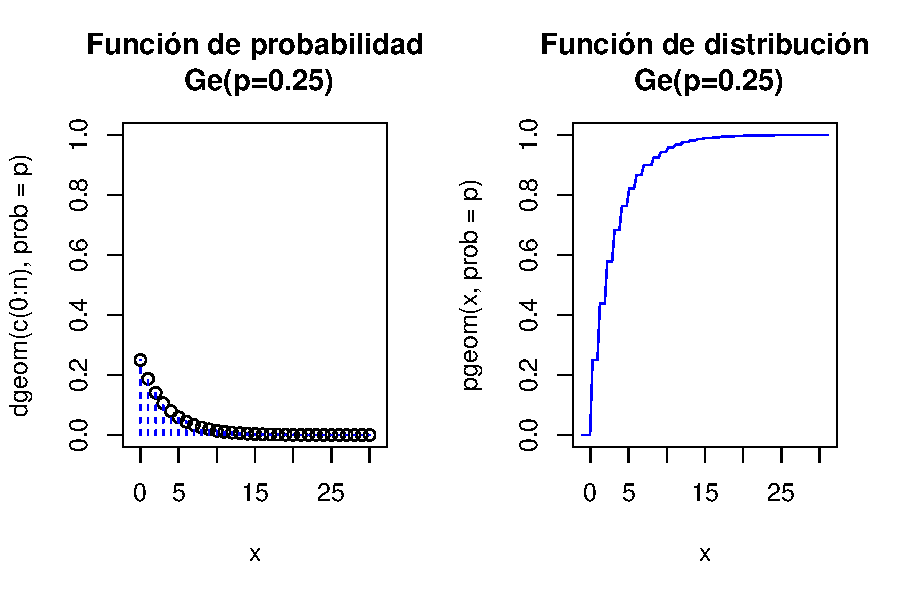
\includegraphics[width=0.8\linewidth,height=\textheight,keepaspectratio]{distibuciones_notables_1_files/figure-pdf/graficos22-1.pdf}
\end{center}

\section{Cálculos con python}\label{cuxe1lculos-con-python}

Veamos los cálculos básicos con python para la distribución geométrica
\(Ge(p=0.25)\). scipy.stats implementa la distribución geométrica que
cuenta el número intentos así que empieza en 1

Cargamos la función de la librería

\begin{Shaded}
\begin{Highlighting}[]
\ImportTok{from}\NormalTok{ scipy.stats }\ImportTok{import}\NormalTok{ geom}
\end{Highlighting}
\end{Shaded}

\section{Cálculos con python}\label{cuxe1lculos-con-python-1}

La función de probabilidad es \texttt{geom.pmf(x,p,loc=0)=geom.pmf(x,p)}
es un geométrica que cuenta el número de intentos para obtener el primer
éxito el valor por defecto del último parámetro es \texttt{loc=0}.

Si queremos la que cuenta el número de fracasos para obtener el primer
éxito (la geométrica que empieza en 0) tenemos que usar
\texttt{geom.pmf(x,p,loc=-1)}.

Es decir \texttt{geom.pmf(x,p,loc=-1)=geom.pmf(x-1,p,loc=0)}

Veamos pues los cálculos para la \(Ge(p)\) que empieza en \(0\).

\(P(X=0)=(1-0.25)^0\cdot 0.25^1=0.25\)

\begin{Shaded}
\begin{Highlighting}[]
\NormalTok{geom.pmf(}\DecValTok{0}\NormalTok{,p}\OperatorTok{=}\FloatTok{0.25}\NormalTok{,loc}\OperatorTok{={-}}\DecValTok{1}\NormalTok{)}
\end{Highlighting}
\end{Shaded}

\begin{verbatim}
0.25
\end{verbatim}

\(P(X\leq 0)=1- (1-0.25)^{0+1}=1-0.75=0.25\)

\begin{Shaded}
\begin{Highlighting}[]
\NormalTok{geom.cdf(}\DecValTok{0}\NormalTok{,p}\OperatorTok{=}\FloatTok{0.25}\NormalTok{,loc}\OperatorTok{={-}}\DecValTok{1}\NormalTok{)}
\end{Highlighting}
\end{Shaded}

\begin{verbatim}
0.24999999999999997
\end{verbatim}

\(P(X\leq 4)=1-(1-0.25)^{4+1}=1-0.75=1-0.75^5=0.7626953.\)

\begin{Shaded}
\begin{Highlighting}[]
\NormalTok{geom.cdf(}\DecValTok{4}\NormalTok{,p}\OperatorTok{=}\FloatTok{0.25}\NormalTok{,loc}\OperatorTok{={-}}\DecValTok{1}\NormalTok{)}
\end{Highlighting}
\end{Shaded}

\begin{verbatim}
0.7626953125
\end{verbatim}

Una muestra aleatoria de tamaño 25 de una \(Ge(0.25)\)

\begin{Shaded}
\begin{Highlighting}[]
\NormalTok{geom.rvs(p}\OperatorTok{=}\FloatTok{0.25}\NormalTok{, size}\OperatorTok{=}\DecValTok{20}\NormalTok{, loc}\OperatorTok{={-}}\DecValTok{1}\NormalTok{)}
\end{Highlighting}
\end{Shaded}

\begin{verbatim}
array([ 9,  2,  2,  4, 17,  1,  5,  2,  1,  2,  2,  3,  1,  0,  1,  0,  4,
        1,  0,  3], dtype=int64)
\end{verbatim}

\section{Cálculos con python}\label{cuxe1lculos-con-python-2}

\textbf{Ejercicio}

Qué probabilidades son las que calcula el siguiente código y qué tipo de
variables geométricas son?

\begin{Shaded}
\begin{Highlighting}[]
\NormalTok{geom.cdf(}\BuiltInTok{range}\NormalTok{(}\DecValTok{5}\NormalTok{),p}\OperatorTok{=}\FloatTok{0.3}\NormalTok{,loc}\OperatorTok{=}\DecValTok{0}\NormalTok{)}
\end{Highlighting}
\end{Shaded}

\begin{verbatim}
array([0.    , 0.3   , 0.51  , 0.657 , 0.7599])
\end{verbatim}

\begin{Shaded}
\begin{Highlighting}[]
\NormalTok{geom.cdf(}\BuiltInTok{range}\NormalTok{(}\DecValTok{5}\NormalTok{),p}\OperatorTok{=}\FloatTok{0.3}\NormalTok{,loc}\OperatorTok{={-}}\DecValTok{1}\NormalTok{)}
\end{Highlighting}
\end{Shaded}

\begin{verbatim}
array([0.3    , 0.51   , 0.657  , 0.7599 , 0.83193])
\end{verbatim}

\section{Cálculos con python esperanza y
varianza}\label{cuxe1lculos-con-python-esperanza-y-varianza}

Con python también podemos calcular directamente algunos parámetros
asociado a una función de distribución predefinida

\begin{Shaded}
\begin{Highlighting}[]
\NormalTok{geom.stats(p}\OperatorTok{=}\FloatTok{0.25}\NormalTok{, loc}\OperatorTok{=}\DecValTok{0}\NormalTok{, moments}\OperatorTok{=}\StringTok{\textquotesingle{}mv\textquotesingle{}}\NormalTok{)}
\end{Highlighting}
\end{Shaded}

\begin{verbatim}
(array(4.), array(12.))
\end{verbatim}

\begin{Shaded}
\begin{Highlighting}[]
\NormalTok{geom.stats(p}\OperatorTok{=}\FloatTok{0.25}\NormalTok{, loc}\OperatorTok{={-}}\DecValTok{1}\NormalTok{, moments}\OperatorTok{=}\StringTok{\textquotesingle{}mv\textquotesingle{}}\NormalTok{)}
\end{Highlighting}
\end{Shaded}

\begin{verbatim}
(array(3.), array(12.))
\end{verbatim}

\section{Cálculos con python esperanza y
varianza}\label{cuxe1lculos-con-python-esperanza-y-varianza-1}

\textbf{Ejercicio}

Comprobad que las medias y las varianzas calculadas en el código
anterior, corresponden a una \(Ge(p=0.3)\) empezando en \(1\) y a una
\(Ge(p=0.3)\) empezando en \(0\).

¿Son las varianzas siempre iguales?

\section{Gráficos con python}\label{gruxe1ficos-con-python}

\begin{Shaded}
\begin{Highlighting}[]
\NormalTok{p }\OperatorTok{=} \FloatTok{0.25}
\NormalTok{x }\OperatorTok{=}\NormalTok{ np.arange(geom.ppf(}\FloatTok{0.01}\NormalTok{, p),geom.ppf(}\FloatTok{0.99}\NormalTok{, p))}
\NormalTok{fig }\OperatorTok{=}\NormalTok{plt.figure(figsize}\OperatorTok{=}\NormalTok{(}\DecValTok{5}\NormalTok{, }\FloatTok{2.7}\NormalTok{))}
\NormalTok{ax }\OperatorTok{=}\NormalTok{ fig.add\_subplot(}\DecValTok{1}\NormalTok{,}\DecValTok{2}\NormalTok{,}\DecValTok{1}\NormalTok{)}
\NormalTok{ax.plot(x, geom.pmf(x, p), }\StringTok{\textquotesingle{}bo\textquotesingle{}}\NormalTok{, ms}\OperatorTok{=}\DecValTok{5}\NormalTok{, label}\OperatorTok{=}\StringTok{\textquotesingle{}geom pmf\textquotesingle{}}\NormalTok{)}
\NormalTok{ax.vlines(x, }\DecValTok{0}\NormalTok{, geom.pmf(x, p), colors}\OperatorTok{=}\StringTok{\textquotesingle{}b\textquotesingle{}}\NormalTok{, lw}\OperatorTok{=}\DecValTok{2}\NormalTok{, alpha}\OperatorTok{=}\FloatTok{0.5}\NormalTok{)}
\ControlFlowTok{for}\NormalTok{ tick }\KeywordTok{in}\NormalTok{ ax.xaxis.get\_major\_ticks():}
\NormalTok{  tick.label.set\_fontsize(}\DecValTok{5}\NormalTok{)}
\ControlFlowTok{for}\NormalTok{ tick }\KeywordTok{in}\NormalTok{ ax.yaxis.get\_major\_ticks():}
\NormalTok{  tick.label.set\_fontsize(}\DecValTok{5}\NormalTok{) }
\NormalTok{ax }\OperatorTok{=}\NormalTok{ fig.add\_subplot(}\DecValTok{1}\NormalTok{,}\DecValTok{2}\NormalTok{,}\DecValTok{2}\NormalTok{)}
\NormalTok{ax.plot(x, geom.cdf(x, p), }\StringTok{\textquotesingle{}bo\textquotesingle{}}\NormalTok{, ms}\OperatorTok{=}\DecValTok{5}\NormalTok{, label}\OperatorTok{=}\StringTok{\textquotesingle{}geom pmf\textquotesingle{}}\NormalTok{)}
\NormalTok{ax.vlines(x, }\DecValTok{0}\NormalTok{, geom.cdf(x, p), colors}\OperatorTok{=}\StringTok{\textquotesingle{}b\textquotesingle{}}\NormalTok{, lw}\OperatorTok{=}\DecValTok{2}\NormalTok{, alpha}\OperatorTok{=}\FloatTok{0.5}\NormalTok{)}
\ControlFlowTok{for}\NormalTok{ tick }\KeywordTok{in}\NormalTok{ ax.xaxis.get\_major\_ticks():}
\NormalTok{  tick.label.set\_fontsize(}\DecValTok{5}\NormalTok{)}
\ControlFlowTok{for}\NormalTok{ tick }\KeywordTok{in}\NormalTok{ ax.yaxis.get\_major\_ticks():}
\NormalTok{  tick.label.set\_fontsize(}\DecValTok{5}\NormalTok{)}
\NormalTok{fig.suptitle(}\StringTok{\textquotesingle{}Distribucion Geometrica\textquotesingle{}}\NormalTok{)}
\NormalTok{plt.show()}
\end{Highlighting}
\end{Shaded}

\section{Gráficos con python}\label{gruxe1ficos-con-python-1}

\begin{center}
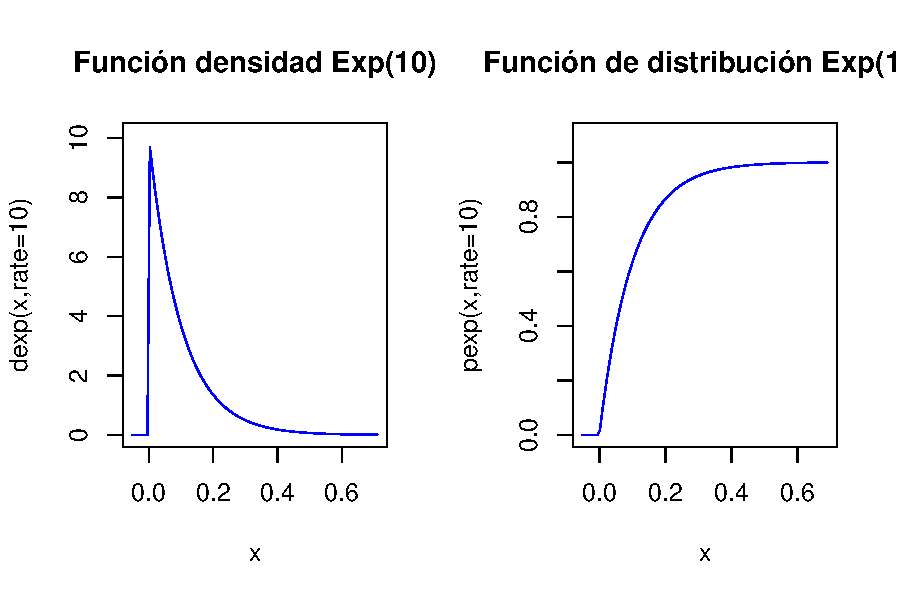
\includegraphics[width=0.7\linewidth,height=\textheight,keepaspectratio]{distibuciones_notables_1_files/figure-pdf/unnamed-chunk-20-1.pdf}
\end{center}

\chapter{Distribución binomial
negativa}\label{distribuciuxf3n-binomial-negativa}

\section{El problema de la puerta con dos
cerraduras}\label{el-problema-de-la-puerta-con-dos-cerraduras}

Supongamos que disponemos de 10 llaves distintas y tenemos que abrir una
puerta con \textbf{dos cerraduras}.

Comenzamos por la primera cerradura, de tal forma que cada vez olvidamos
qué llave hemos probado.

Una vez abierta la primera cerradura probamos de igual forma con la
segunda hasta que también la abrimos.

Sea \(X=\) la v.a. que cuenta el número de fracasos hasta abrir la
puerta.

Acertar una llave de la puerta es un experimento Bernoulli con
probabilidad de éxito \(p=0.1\). Lo repetiremos hasta obtener 2 éxitos.

\section{Distribución binomial
negativa}\label{distribuciuxf3n-binomial-negativa-1}

En general tendremos un experimento de Bernoulli con probabilidad de
éxito \(0<p<1\) tal que:

\begin{itemize}
\tightlist
\item
  Repetimos el experimento hasta obtener el \(n\)-ésimo éxito ¡¡abrir la
  maldita puerta!!.
\item
  Sea \(X\) la v.a. que cuenta el número fallos hasta abrir la puerta,
  es decir, hasta conseguir el n-ésimo éxito. Notemos que no contamos
  los éxitos, solo contamos los fracasos
\end{itemize}

\section{Distribución binomial
negativa}\label{distribuciuxf3n-binomial-negativa-2}

Si representamos como es habitual un suceso como una cadena de F's y
E's, para \(n=2\), algunos sucesos elementales serán:
\[\small{\{EE,FEE,EFE, FFEE,FEFE,EFFE,FFFEE,FFEFE,FEFFE,EFFFE\}.}\]

Calculemos algunas probabilidades para \(n=2\): \[
\small{
\begin{array}{rl}
P(X=0) & =P(\{EE\})=p^2, \\
P(X=1) & =P(\{FEE,EFE\})=2\cdot (1-p)\cdot p^2, \\
P(X=2) & =P(\{FFEE,FEFE,EFFE\})=3\cdot (1-p)^2\cdot p^2, \\
P(X=3) & =P(\{FFFEE,FFEFE,FEFFE,EFFFE\})=4\cdot (1-p)^3\cdot p^2.
\end{array}
}
\]

\section{Distribución binomial
negativa}\label{distribuciuxf3n-binomial-negativa-3}

En general su función de probabilidad es

\[
P_{X}(k)=P(X=k)=\left\{\begin{array}{ll}
     {k+n-1\choose n-1} \cdot (1-p)^{k}\cdot p^n & \mbox{si } k=0,1,\ldots\\
     0 & \mbox{en otro caso}\end{array}\right.
\]

\section{Distribución binomial
negativa}\label{distribuciuxf3n-binomial-negativa-4}

Una v.a. con este tipo de distribución recibe el nombre de
\textbf{binomial negativa} y la denotaremos por \(BN(n,p)\).

Notemos que \(BN(1,p)=Ge(p)\).

\section{Distribución binomial
negativa}\label{distribuciuxf3n-binomial-negativa-5}

\textbf{Demostración}

Justifiquemos el resultado. Sea \(X\) una \(BN(n,p)\) y sea
\(k=0,1,2,\ldots\).

\[\scriptsize{P(X=k)=P(\mbox{Todas las cadenas de E's y F' con $k$ F, con $n$ E y acabadas en E})}\]

\[
\scriptsize{\overbrace{\underbrace{\overbrace{EFFF\ldots EEF}^{n-1 \quad \mbox{Éxitos}.}}}_{k \quad\mbox{Fracasos}}^{k+n-1\mbox{ posiciones}}E}
\]

De estas cadenas hay tantas como maneras de elegir de entre las
\(k+n-1\) primeras posiciones \(n-1\) para colocar los éxitos. Esta
cantidad es el número binomial \({k+n-1\choose n-1}.\)

\section{Números binomiales
negativos}\label{nuxfameros-binomiales-negativos}

Números binomiales negativos

Dados dos enteros positivos \(n\) y \(k\) se define el número binomial
negativo como

\[\binom{-n}{k}=\frac{(-n)(-n-1)\cdots (-n-k+1)}{k!}.\]

Los números binomiales negativos generalizan la fórmula de Newton para
exponentes negativos: \[
(t+1)^{-n}=\sum_{k=0}^{+\infty}\left(\begin{array}{c} -n
\\ k\end{array}\right) t^{k}
\]

\section{Números binomiales
negativos}\label{nuxfameros-binomiales-negativos-1}

\texttt{R} usa la función \texttt{choose} para calcular números
binomiales, sean negativos o no. Veámoslo con un ejemplo:

\[
\begin{array}{rl}
{-6\choose 4}&=\frac{-6\cdot (-6-1)\cdot \cdot (-6-2)\cdot (-6-3) }{4!}\\
&=  \frac{-6\cdot(-7)\cdot (-8)\cdot (-9)}{24}\\
&= \frac{3024}{24}=126.
\end{array}
\]

Si realizamos el cálculo con \texttt{R} obtenemos el mismo resultado:

\begin{Shaded}
\begin{Highlighting}[]
\FunctionTok{choose}\NormalTok{(}\SpecialCharTok{{-}}\DecValTok{6}\NormalTok{,}\DecValTok{4}\NormalTok{)}
\end{Highlighting}
\end{Shaded}

\begin{verbatim}
[1] 126
\end{verbatim}

\section{\texorpdfstring{Esperanza de una
\(BN(n,p)\)}{Esperanza de una BN(n,p)}}\label{esperanza-de-una-bnnp}

Su \textbf{esperanza es}

\[E(X)=\sum_{k=0}^{+\infty} k\cdot {k+n-1\choose n-1} \cdot (1-p)^{k}\cdot p^n=n\cdot\frac{1-p}{p}.\]

La \textbf{esperanza de \(X^2\) es}

\[E(X^2)=\sum_{k=0}^{+\infty} k^2\cdot {k+n-1\choose n-1} \cdot (1-p)^{k}\cdot p^n=n\cdot\frac{1-p}{p^2}+\left(n\cdot \frac{1-p}{p}\right)^2.\]

\section{\texorpdfstring{Varianza de una
\(BN(n,p)\)}{Varianza de una BN(n,p)}}\label{varianza-de-una-bnnp}

Por último la \textbf{varianza es}

\[
Var(X)=E(X^2)-E(X)^2=
\]

\[=n\cdot \frac{1-p}{p^2}+\left(n\cdot \frac{1-p}{p}\right)^2-\left(n\cdot \frac{1-p}{p}\right)^2=
n\cdot \frac{1-p}{p^2}.\]

y por tanto la desviación típica es

\[\sqrt{Var(X)} = \frac{\sqrt{n(1-p)}}{p}\]

\section{\texorpdfstring{Resumen distribución Binomial Negativa
\(BN(n,p)\)}{Resumen distribución Binomial Negativa BN(n,p)}}\label{resumen-distribuciuxf3n-binomial-negativa-bnnp}

\renewcommand{\arraystretch}{1.8}
\begin{table}
\centering
\begin{tabular}{|l|}
\hline\rowcolor{LightBlue}
 $X=$ Número de fracasos antes de conseguir el $n$-ésimo éxito, $P(\mbox{Éxito})=p$. $BN(n,p)$ 
\\\hline
$D_X=\{0,1,2,3\ldots\}$  \\\hline
$P_X(k)=P(X=k)=\left\{\begin{array}{ll} {k+n-1\choose n-1} \cdot (1-p)^{k}\cdot p^n, & \mbox{si }  k=0,1,\ldots \\ 0, & \mbox{en otro caso.}\end{array}\right.$\\\hline
$
F_X(x)=P(X\leq x)=
\left\{
\begin{array}{ll} 0, & \mbox{si } x<0\\\displaystyle\sum_{i=0}^{k} P(X=i) & \mbox{si  }\left\{\begin{array}{l}k\leq x< k+1,\\k=0,1,2,\ldots\end{array}\right.\end{array}\right.$ 
\\\hline
$E(X)=n\cdot\frac{1-p}{p}$;  $Var(X)=n\cdot \frac{1-p}{p^2}.$ \\\hline
\end{tabular}
\end{table}

\section{\texorpdfstring{Ejemplo puerta dos cerraduras
\(BN(n=2,p=0.1)\).}{Ejemplo puerta dos cerraduras BN(n=2,p=0.1).}}\label{ejemplo-puerta-dos-cerraduras-bnn2p0.1.}

\textbf{Ejercicio: Puerta con dos cerraduras}

Recordemos nuestra puerta con dos cerraduras que se abren
secuencialmente. Tenemos un manojo de 10 llaves casi idénticas de manera
que cada vez que probamos una llave olvidamos qué llave hemos usado.

Sea \(X\) la v.a que nos da el número de intentos fallidos hasta abrir
abrir la puerta.

\section{\texorpdfstring{Ejemplo
\(BN(n,p)\)}{Ejemplo BN(n,p)}}\label{ejemplo-bnnp}

Estamos interesado en modelar este problema. La preguntas son:

\begin{enumerate}
\def\labelenumi{\arabic{enumi}.}
\tightlist
\item
  ¿Cuál es la distribución de probabilidad de \(X\) la v.a que nos da el
  número fallos hasta abrir la puerta?
\item
  ¿Cuál es la función de probabilidad y de distribución de \(X\)?
\item
  ¿Cuál es la probabilidad de fallar exactamente 5 veces antes de abrir
  la puerta?
\item
  ¿Cuál es la probabilidad de fallar más de 4?
\item
  ¿Cuál es el número esperado de fallos? ¿Y su desviación típica?
\end{enumerate}

\section{\texorpdfstring{Ejemplo dos cerraduras
\(BN(n=2,p=0.1)\).}{Ejemplo dos cerraduras BN(n=2,p=0.1).}}\label{ejemplo-dos-cerraduras-bnn2p0.1.}

\textbf{Solución 1.} ¿Cuál es la distribución de probabilidad de \(X\)
la v.a que nos da el número fallos hasta abrir la puerta?

Bajo estados condiciones tenemos que la probabilidad de ``éxito'' de
cada intento es \(p=\frac{1}{10}=0.1\). Como cada vez \emph{olvidamos}
qué llave hemos probado, cada intento será independiente del anterior.

Así que la variable \(X\) que queremos modelar cuenta el número fallos
de repeticiones sucesivas e independientes de un experimento
\(Ber(p=0.1)\) hasta conseguir 2 éxitos en un experimento.

Por lo tanto podemos asegurar que \(X\) sigue un distribución
\(BN(n=2,p=0.1).\)

\section{\texorpdfstring{Ejemplo
\(BN(n=2,p=0.1)\)}{Ejemplo BN(n=2,p=0.1)}}\label{ejemplo-bnn2p0.1}

\textbf{Solución 2.} ¿Cuál es la función de probabilidad y de
distribución del \(X\)?

En general la función de probabilidad de una \(BN(n,p)\) es

\[
P_X(k)=P(X=k)=
\left\{
\begin{array}{cc} 
{k+n-1\choose n-1} \cdot (1-p)^{k}\cdot p^n & \mbox{si }  k=0,1,\ldots \\ 0 & \mbox{en otro caso.}\end{array}\right.
\]

Si aplicamos la expresión anterior para \(n=2\) y \(p=0.1\), obtenemos:
\[
P_X(k)=P(X=k)=
\left\{
\begin{array}{cc} 
{k+2-1\choose 2-1} \cdot 0.9^{k}\cdot 0.1^2 & \mbox{si }  k=0,1,2,\ldots \\ 0 & \mbox{en otro caso.}\end{array}\right.
\]

\section{\texorpdfstring{Ejemplo
\(BN(n=2,p=0.1)\)}{Ejemplo BN(n=2,p=0.1)}}\label{ejemplo-bnn2p0.1-1}

Simplificando

\[
P_X(X=k)=P(X=k)=
\left\{
\begin{array}{cc} 
0.01\cdot (k+1)\cdot 0.9^{k}, & \mbox{si }  k=0,1,2,\ldots \\ 0 & \mbox{en otro caso.}\end{array}\right.
\]

La función de distribución en general es

\[
F_X(x)=P(X\leq x)=
\left\{
\begin{array}{ll}
0 & \mbox{si } x<0 \\
\displaystyle\sum_{i=0}^{k }{i+n-1\choose n-1} \cdot (1-p)^{i+n-1}\cdot p^n 
& \mbox{si }\left\{\begin{array}{l} k\leq x< k+1\\k=0,1,2,\ldots\end{array}\right. 
\end{array}
\right.
\]

\section{\texorpdfstring{Ejemplo
\(BN(n=2,p=0.1)\)}{Ejemplo BN(n=2,p=0.1)}}\label{ejemplo-bnn2p0.1-2}

Simplificando para \(n=2\), \(p=0.1\).

\[
F_X(x)=P(X\leq x)=
\left\{
\begin{array}{ll}
0, & \mbox{si } x<0, \\
\displaystyle\sum_{i=0}^{k }0.01\cdot (i+1) \cdot 0.9^{i+1},
& \mbox{si }\left\{\begin{array}{l} k\leq x< k+1,\\k=0,1,2,\ldots\end{array}\right. 
\end{array}
\right.
\]

\textbf{Solución 3.} ¿Cuál es la probabilidad de fallar exactamente 5
veces antes de abrir la puerta?

\[
P(X=5)= 0.01\cdot (5+1) \cdot 0.9^{5}= 0.06 \cdot 0.9^{5}= 0.0354294.
\]

\section{\texorpdfstring{Ejemplo
\(BN(n=2,p=0.1)\)}{Ejemplo BN(n=2,p=0.1)}}\label{ejemplo-bnn2p0.1-3}

\textbf{Solución 4.} ¿Cuál es la probabilidad de fallar más de 4?

Nos piden que\\
\[
P(X>4)=1-P(X\leq 4).
\]

Calculemos primero \(P(X\leq 4):\)

\[
\begin{array}{rl}
P(X\leq 4) &=  \displaystyle\sum_{x=0}^{4} P(X=x)=P(X=0)+P(X=1)+P(X=2)+P(X=3)+P(X=4)\\
&= 0.01\cdot (0+1) \cdot 0.9^{0}+0.01\cdot (1+1) \cdot 0.9^{1}+0.01\cdot (2+1) \cdot 0.9^{2} \\ &\ \ 
+0.01\cdot (3+1) \cdot 0.9^{3} + 0.01\cdot (4+1) \cdot 0.9^{4} \\ & =
0.01 +0.018+0.0243+0.02916+0.032805 = 0.114265.
\end{array}
\]

\section{\texorpdfstring{Ejemplo
\(BN(n=2,p=0.1)\)}{Ejemplo BN(n=2,p=0.1)}}\label{ejemplo-bnn2p0.1-4}

Por lo tanto

\[
P(X>4)=1-P(X\leq 4)=1-0.114265=
0.885735.
\]

\textbf{Solución 5.} ¿Cuál es el número esperado de fallos? ¿Y su
desviación típica?

Como \(X\) sigue una ley \(BN(n=2,p=0.1)\)

\[E(X)=n\cdot \frac{1-p}{p}=2\cdot \frac{1-0.1}{0.1}=18.\]

El número de fallos esperado es 18. La varianza es

\[
Var(X)=n\cdot\frac{1-p}{p^2}=2 \cdot \frac{1-0.1}{0.1^2}=180,
\]

y su desviación típica \(\sqrt{180}=13.41641.\)

\section{Cálculos con R}\label{cuxe1lculos-con-r-2}

La función de \texttt{R} que calcula la función de probabilidad de la
binomial negativa con sus parámetros básicos es:

\begin{verbatim}
dnbinom(x, size, prob,...)`
\end{verbatim}

donde \texttt{size} (\(n\)) es el número de éxitos y \texttt{prob}
(\(p\)), la probabilidad de éxito.

Así en el ejemplo de la puerta con dos cerraduras, \(X\) es una
\(BN(n=size=2,p=prob=0.1)\). Por ejemplo, \(P(X=5)\) que hemos calculado
en el ejemplo anterior, vale:

\begin{Shaded}
\begin{Highlighting}[]
\FunctionTok{dnbinom}\NormalTok{(}\DecValTok{5}\NormalTok{,}\AttributeTok{size=}\DecValTok{2}\NormalTok{,}\AttributeTok{p=}\FloatTok{0.1}\NormalTok{)}
\end{Highlighting}
\end{Shaded}

\begin{verbatim}
[1] 0.0354294
\end{verbatim}

\section{Cálculos con R}\label{cuxe1lculos-con-r-3}

De forma similar calculamos calculamos \(P(X\leq 4)\),
\(P(X>4)=1-P(X\leq 4)\) y \(P(X>4)\).

\begin{Shaded}
\begin{Highlighting}[]
\FunctionTok{pnbinom}\NormalTok{(}\DecValTok{4}\NormalTok{,}\AttributeTok{size=}\DecValTok{2}\NormalTok{,}\AttributeTok{p=}\FloatTok{0.1}\NormalTok{)}
\end{Highlighting}
\end{Shaded}

\begin{verbatim}
[1] 0.114265
\end{verbatim}

\begin{Shaded}
\begin{Highlighting}[]
\DecValTok{1}\SpecialCharTok{{-}}\FunctionTok{pnbinom}\NormalTok{(}\DecValTok{4}\NormalTok{,}\AttributeTok{size=}\DecValTok{2}\NormalTok{,}\AttributeTok{p=}\FloatTok{0.1}\NormalTok{)}
\end{Highlighting}
\end{Shaded}

\begin{verbatim}
[1] 0.885735
\end{verbatim}

\begin{Shaded}
\begin{Highlighting}[]
\FunctionTok{pnbinom}\NormalTok{(}\DecValTok{4}\NormalTok{,}\AttributeTok{size=}\DecValTok{2}\NormalTok{,}\AttributeTok{p=}\FloatTok{0.1}\NormalTok{,}\AttributeTok{lower.tail=}\ConstantTok{FALSE}\NormalTok{)}
\end{Highlighting}
\end{Shaded}

\begin{verbatim}
[1] 0.885735
\end{verbatim}

\section{Cálculos con python}\label{cuxe1lculos-con-python-3}

La función con python es \texttt{nbinom.pmf(k,\ n,\ p,\ loc)}. Hay que
cargarla desde \texttt{scpi.stats}

\begin{Shaded}
\begin{Highlighting}[]
\ImportTok{from}\NormalTok{ scipy.stats }\ImportTok{import}\NormalTok{ nbinom}
\end{Highlighting}
\end{Shaded}

Recordemos que de nuevo se cumple que

\begin{Shaded}
\begin{Highlighting}[]
\NormalTok{nbinom.pmf(k, n, p, loc) }\OperatorTok{=}\NormalTok{ nbinom.pmf(k}\OperatorTok{{-}}\NormalTok{loc, n, p)\textasciigrave{}}
\end{Highlighting}
\end{Shaded}

\section{\texorpdfstring{Cálculos \(BN(n,p)\) con
python}{Cálculos BN(n,p) con python}}\label{cuxe1lculos-bnnp-con-python}

\begin{Shaded}
\begin{Highlighting}[]
\NormalTok{nbinom.pmf(k}\OperatorTok{=}\DecValTok{5}\NormalTok{,n}\OperatorTok{=}\DecValTok{2}\NormalTok{,p}\OperatorTok{=}\FloatTok{0.1}\NormalTok{)}
\end{Highlighting}
\end{Shaded}

\begin{verbatim}
0.0354294
\end{verbatim}

\begin{Shaded}
\begin{Highlighting}[]
\NormalTok{nbinom.pmf(k}\OperatorTok{=}\DecValTok{5}\NormalTok{,n}\OperatorTok{=}\DecValTok{2}\NormalTok{,p}\OperatorTok{=}\FloatTok{0.1}\NormalTok{,loc}\OperatorTok{=}\DecValTok{0}\NormalTok{)}
\end{Highlighting}
\end{Shaded}

\begin{verbatim}
0.0354294
\end{verbatim}

\begin{Shaded}
\begin{Highlighting}[]
\NormalTok{nbinom.cdf(k}\OperatorTok{=}\DecValTok{4}\NormalTok{,n}\OperatorTok{=}\DecValTok{2}\NormalTok{,p}\OperatorTok{=}\FloatTok{0.1}\NormalTok{)}
\end{Highlighting}
\end{Shaded}

\begin{verbatim}
0.11426500000000002
\end{verbatim}

\begin{Shaded}
\begin{Highlighting}[]
\DecValTok{1}\OperatorTok{{-}}\NormalTok{nbinom.cdf(k}\OperatorTok{=}\DecValTok{4}\NormalTok{,n}\OperatorTok{=}\DecValTok{2}\NormalTok{,p}\OperatorTok{=}\FloatTok{0.1}\NormalTok{)}
\end{Highlighting}
\end{Shaded}

\begin{verbatim}
0.8857349999999999
\end{verbatim}

\section{\texorpdfstring{Cálculos \(BN(n,p)\) con
python}{Cálculos BN(n,p) con python}}\label{cuxe1lculos-bnnp-con-python-1}

Generemos 100 observaciones aleatorias de una \(BN(n=2,0.1)\). Es decir
serán las veces que hemos fallado hasta abrir la puerta 100 veces.

\begin{Shaded}
\begin{Highlighting}[]
\NormalTok{nbinom.rvs(n}\OperatorTok{=}\DecValTok{2}\NormalTok{, p}\OperatorTok{=}\FloatTok{0.1}\NormalTok{, size}\OperatorTok{=}\DecValTok{100}\NormalTok{)}
\end{Highlighting}
\end{Shaded}

\begin{verbatim}
array([11, 15,  7, 34,  9,  1, 25, 15, 16, 34, 17, 19,  1, 31, 17, 16,  7,
       12, 10,  7,  4, 24,  4,  8,  8, 21, 16,  1, 10,  5, 14,  4,  3, 11,
       15, 13, 57,  4, 13, 21,  2, 17,  7, 16, 46, 12,  6,  9,  3, 20, 12,
       23,  9,  9,  5, 19, 41, 39, 44, 42, 14, 13, 32,  1, 17, 35, 13, 33,
        5, 17, 30, 60,  7,  3,  8, 12,  4, 43,  2,  6, 21, 25, 15,  7, 36,
       18, 32, 27,  8,  2, 34,  5, 40, 12,  5, 15, 16, 13,  7, 35],
      dtype=int64)
\end{verbatim}

\section{\texorpdfstring{Cálculos \(BN(n,p)\) con
python}{Cálculos BN(n,p) con python}}\label{cuxe1lculos-bnnp-con-python-2}

La \textbf{esperanza} y la \textbf{varianza}de una \(BN(n=2,0.1)\)
valen:

\begin{Shaded}
\begin{Highlighting}[]
\NormalTok{n, p}\OperatorTok{=}\DecValTok{2}\NormalTok{,}\FloatTok{0.1}
\NormalTok{params }\OperatorTok{=}\NormalTok{ nbinom.stats(n,p,moments}\OperatorTok{=}\StringTok{\textquotesingle{}mv\textquotesingle{}}\NormalTok{)}
\BuiltInTok{print}\NormalTok{(}\StringTok{"E(X)=}\SpecialCharTok{\{m\}}\StringTok{"}\NormalTok{.}\BuiltInTok{format}\NormalTok{(m}\OperatorTok{=}\NormalTok{params[}\DecValTok{0}\NormalTok{]))}
\end{Highlighting}
\end{Shaded}

\begin{verbatim}
E(X)=18.0
\end{verbatim}

\begin{Shaded}
\begin{Highlighting}[]
\BuiltInTok{print}\NormalTok{(}\StringTok{"Var(X)=}\SpecialCharTok{\{v\}}\StringTok{"}\NormalTok{.}\BuiltInTok{format}\NormalTok{(v}\OperatorTok{=}\NormalTok{params[}\DecValTok{1}\NormalTok{]))}
\end{Highlighting}
\end{Shaded}

\begin{verbatim}
Var(X)=179.99999999999997
\end{verbatim}

\section{Gráficas de la binomial negativa con
R}\label{gruxe1ficas-de-la-binomial-negativa-con-r}

El siguiente código de R dibuja las función de probabilidad y la de
distribución de una \(BN(n=2,p=0.1)\)

\begin{Shaded}
\begin{Highlighting}[]
\FunctionTok{par}\NormalTok{(}\AttributeTok{mfrow=}\FunctionTok{c}\NormalTok{(}\DecValTok{1}\NormalTok{,}\DecValTok{2}\NormalTok{))}
\NormalTok{aux}\OtherTok{=}\FunctionTok{rep}\NormalTok{(}\DecValTok{0}\NormalTok{,}\DecValTok{22}\NormalTok{)}
\NormalTok{aux[}\FunctionTok{seq}\NormalTok{(}\DecValTok{2}\NormalTok{,}\DecValTok{22}\NormalTok{,}\DecValTok{2}\NormalTok{)]}\OtherTok{=}\FunctionTok{dnbinom}\NormalTok{(}\FunctionTok{c}\NormalTok{(}\DecValTok{0}\SpecialCharTok{:}\DecValTok{10}\NormalTok{),}\AttributeTok{size=}\DecValTok{2}\NormalTok{,}\AttributeTok{prob=}\FloatTok{0.1}\NormalTok{)}
\FunctionTok{plot}\NormalTok{(}\AttributeTok{x=}\FunctionTok{c}\NormalTok{(}\DecValTok{0}\SpecialCharTok{:}\DecValTok{10}\NormalTok{),}\AttributeTok{y=}\FunctionTok{dnbinom}\NormalTok{(}\FunctionTok{c}\NormalTok{(}\DecValTok{0}\SpecialCharTok{:}\DecValTok{10}\NormalTok{),}\AttributeTok{size=}\DecValTok{2}\NormalTok{,}\AttributeTok{prob=}\FloatTok{0.1}\NormalTok{),}
  \AttributeTok{ylim=}\FunctionTok{c}\NormalTok{(}\DecValTok{0}\NormalTok{,}\DecValTok{1}\NormalTok{),}\AttributeTok{xlim=}\FunctionTok{c}\NormalTok{(}\SpecialCharTok{{-}}\DecValTok{1}\NormalTok{,}\DecValTok{11}\NormalTok{),}\AttributeTok{xlab=}\StringTok{"x"}\NormalTok{,}
  \AttributeTok{main=}\StringTok{"Función de probabilidad}\SpecialCharTok{\textbackslash{}n}\StringTok{ BN(n=2,p=0.1)"}\NormalTok{)}
\FunctionTok{lines}\NormalTok{(}\AttributeTok{x=}\FunctionTok{rep}\NormalTok{(}\DecValTok{0}\SpecialCharTok{:}\DecValTok{10}\NormalTok{,}\AttributeTok{each=}\DecValTok{2}\NormalTok{),}\AttributeTok{y=}\NormalTok{aux, }\AttributeTok{type =} \StringTok{"h"}\NormalTok{, }\AttributeTok{lty =} \DecValTok{2}\NormalTok{,}\AttributeTok{col=}\StringTok{"blue"}\NormalTok{)}
\FunctionTok{curve}\NormalTok{(}\FunctionTok{pnbinom}\NormalTok{(x,}\AttributeTok{size=}\DecValTok{2}\NormalTok{,}\AttributeTok{prob=}\DecValTok{0}\NormalTok{,}\DecValTok{1}\NormalTok{),}
  \AttributeTok{xlim=}\FunctionTok{c}\NormalTok{(}\SpecialCharTok{{-}}\DecValTok{1}\NormalTok{,}\DecValTok{11}\NormalTok{),}\AttributeTok{col=}\StringTok{"blue"}\NormalTok{,}
  \AttributeTok{main=}\StringTok{"Función de distribución}\SpecialCharTok{\textbackslash{}n}\StringTok{ BN(n=2,p=0.1)"}\NormalTok{)}
\FunctionTok{par}\NormalTok{(}\AttributeTok{mfrow=}\FunctionTok{c}\NormalTok{(}\DecValTok{1}\NormalTok{,}\DecValTok{1}\NormalTok{))}
\end{Highlighting}
\end{Shaded}

\section{Gráficas de la binomial negativa con
R}\label{gruxe1ficas-de-la-binomial-negativa-con-r-1}

\begin{center}
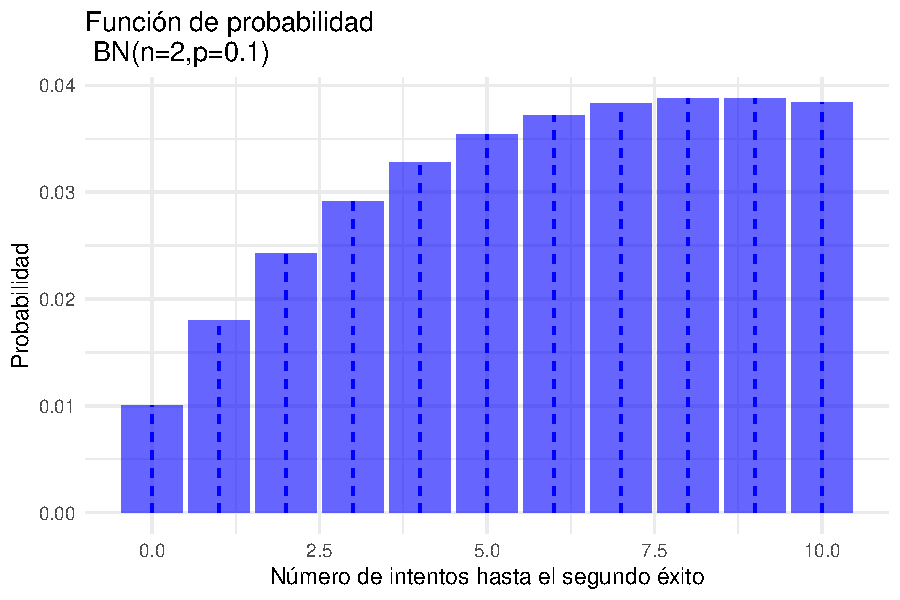
\includegraphics[width=0.7\linewidth,height=\textheight,keepaspectratio]{distibuciones_notables_1_files/figure-pdf/unnamed-chunk-31-1.pdf}
\end{center}

\section{Gráficos de la binomial negativa con
python}\label{gruxe1ficos-de-la-binomial-negativa-con-python}

\textbf{Ejercicio}

Buscad en los manuales de python cómo se dibuja la función de
probabilidad y de distribución de una binomial. negativa

Necesitamos de nuevo más librerías

\begin{Shaded}
\begin{Highlighting}[]
\ImportTok{import}\NormalTok{ numpy }\ImportTok{as}\NormalTok{ np}
\ImportTok{from}\NormalTok{ scipy.stats }\ImportTok{import}\NormalTok{ nbinom}
\ImportTok{import}\NormalTok{ matplotlib.pyplot }\ImportTok{as}\NormalTok{ plt}
\end{Highlighting}
\end{Shaded}

\section{Gráficos de la binomial negativa con
python}\label{gruxe1ficos-de-la-binomial-negativa-con-python-1}

\begin{Shaded}
\begin{Highlighting}[]
\NormalTok{n, p }\OperatorTok{=} \DecValTok{10}\NormalTok{, }\FloatTok{0.25}
\NormalTok{x }\OperatorTok{=}\NormalTok{ np.arange(}\DecValTok{0}\NormalTok{,nbinom.ppf(}\FloatTok{0.99}\NormalTok{, n, p))}
\NormalTok{fig }\OperatorTok{=}\NormalTok{plt.figure(figsize}\OperatorTok{=}\NormalTok{(}\DecValTok{5}\NormalTok{, }\FloatTok{2.7}\NormalTok{))}
\NormalTok{ax }\OperatorTok{=}\NormalTok{ fig.add\_subplot(}\DecValTok{1}\NormalTok{,}\DecValTok{2}\NormalTok{,}\DecValTok{1}\NormalTok{)}
\NormalTok{ax.plot(x, nbinom.pmf(x, n, p), }\StringTok{\textquotesingle{}bo\textquotesingle{}}\NormalTok{, ms}\OperatorTok{=}\DecValTok{5}\NormalTok{, label}\OperatorTok{=}\StringTok{\textquotesingle{}nbinom pmf\textquotesingle{}}\NormalTok{)}
\NormalTok{ax.vlines(x, }\DecValTok{0}\NormalTok{, nbinom.pmf(x, n, p), colors}\OperatorTok{=}\StringTok{\textquotesingle{}b\textquotesingle{}}\NormalTok{, lw}\OperatorTok{=}\DecValTok{2}\NormalTok{, alpha}\OperatorTok{=}\FloatTok{0.5}\NormalTok{)}
\ControlFlowTok{for}\NormalTok{ tick }\KeywordTok{in}\NormalTok{ ax.xaxis.get\_major\_ticks():}
\NormalTok{  tick.label.set\_fontsize(}\DecValTok{5}\NormalTok{)}
\ControlFlowTok{for}\NormalTok{ tick }\KeywordTok{in}\NormalTok{ ax.yaxis.get\_major\_ticks():}
\NormalTok{  tick.label.set\_fontsize(}\DecValTok{5}\NormalTok{) }
\NormalTok{ax }\OperatorTok{=}\NormalTok{ fig.add\_subplot(}\DecValTok{1}\NormalTok{,}\DecValTok{2}\NormalTok{,}\DecValTok{2}\NormalTok{)}
\NormalTok{ax.plot(x, nbinom.cdf(x, n, p), }\StringTok{\textquotesingle{}bo\textquotesingle{}}\NormalTok{, ms}\OperatorTok{=}\DecValTok{5}\NormalTok{, label}\OperatorTok{=}\StringTok{\textquotesingle{}nbinom pmf\textquotesingle{}}\NormalTok{)}
\NormalTok{ax.vlines(x, }\DecValTok{0}\NormalTok{, nbinom.cdf(x, n, p), colors}\OperatorTok{=}\StringTok{\textquotesingle{}b\textquotesingle{}}\NormalTok{, lw}\OperatorTok{=}\DecValTok{2}\NormalTok{, alpha}\OperatorTok{=}\FloatTok{0.5}\NormalTok{)}
\ControlFlowTok{for}\NormalTok{ tick }\KeywordTok{in}\NormalTok{ ax.xaxis.get\_major\_ticks():}
\NormalTok{  tick.label.set\_fontsize(}\DecValTok{5}\NormalTok{)}
\ControlFlowTok{for}\NormalTok{ tick }\KeywordTok{in}\NormalTok{ ax.yaxis.get\_major\_ticks():}
\NormalTok{  tick.label.set\_fontsize(}\DecValTok{5}\NormalTok{)}
\NormalTok{fig.suptitle(}\StringTok{\textquotesingle{}Distribucion Binomial Negativa\textquotesingle{}}\NormalTok{)}
\NormalTok{plt.show()}
\end{Highlighting}
\end{Shaded}

\section{Gráficos de la binomial negativa con
python}\label{gruxe1ficos-de-la-binomial-negativa-con-python-2}

\begin{center}
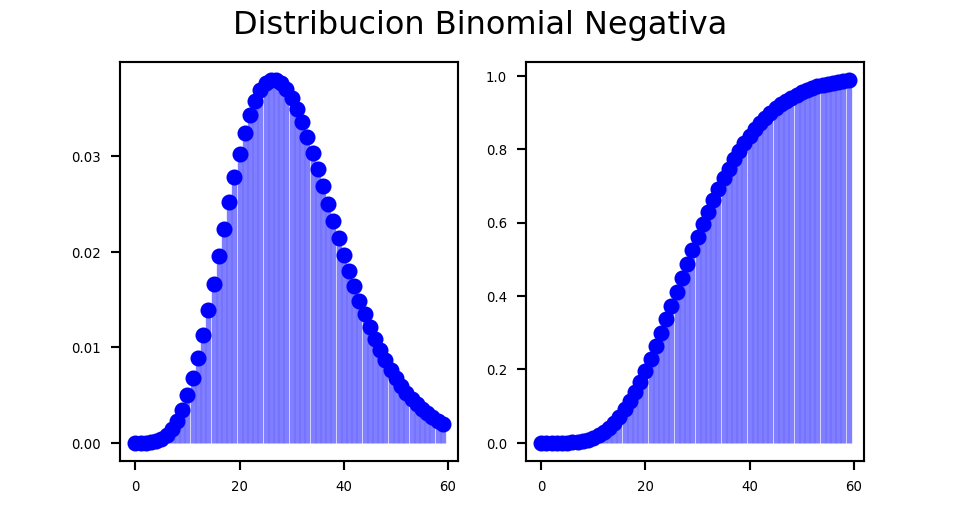
\includegraphics[width=0.7\linewidth,height=\textheight,keepaspectratio]{distibuciones_notables_1_files/figure-pdf/negativa_py_show-1.pdf}
\end{center}

\section{Ejercicio: Acceso aleatorio a un sistema con triple
clave.}\label{ejercicio-acceso-aleatorio-a-un-sistema-con-triple-clave.}

\textbf{Sistema con tres claves de acceso}

Supongamos que tenemos un sistema informático tiene un programa de
seguridad que genera accesos con claves de 3 dígitos
\(000,001,\ldots 999\). En total 1000 posibilidades.

Como una clave de tres dígitos es fácil de romper proponemos considerar
tres claves consecutivas de acceso al sistema, cada una de 3 dígitos.

Para acceder al sistema hay que dar las tres claves de forma consecutiva
y por orden.

Es decir hasta que no averiguamos la primera clave no pasamos a la
segunda clave.

Supongamos que cada vez que ponemos las dos claves olvidamos el
resultado y seguimos poniendo claves al azar hasta adivinar la
contraseña.

Así hasta conseguir entrar en el sistema.

Sea \(X\) la v.a que nos da el número de fallos antes de entrar en el
sistema.

\section{Ejercicio acceso aleatorio a un sistema con triple
clave.}\label{ejercicio-acceso-aleatorio-a-un-sistema-con-triple-clave.-1}

Estamos interesados en modelar este problema. La preguntas son:

\begin{enumerate}
\def\labelenumi{\arabic{enumi}.}
\tightlist
\item
  ¿Cuál es la distribución de probabilidad de \(X\), la v.a que nos da
  el número de fallos antes de acceder al sistema.
\item
  ¿Cuál es la función de probabilidad y de distribución del \(X\)?
\item
  ¿Cuál es la probabilidad de fallar 150 veces antes de acceder en el
  sistema?
\item
  ¿Cuál es la probabilidad de fallar más de 150 veces antes de entrar en
  el sistema?
\item
  ¿Cuál es el número esperado de fallos antes de acceder al sistema? ¿Y
  su varianza?
\end{enumerate}

\section{\texorpdfstring{Ejemplo
\(BN(r,p)\)}{Ejemplo BN(r,p)}}\label{ejemplo-bnrp}

\textbf{Solución 1.} ¿Cuál es la distribución de probabilidad de \(X\),
la v.a que nos da el número de fallos antes de acceder al sistema?

Bajo estados condiciones tenemos que la probabilidad de ``éxito'' de
cada intento es \(p=\frac{1}{1000}=0.001\). Y como cada vez
\emph{olvidamos} en los dígitos cada intento será independiente del
anterior.

Así que la variable \(X\) cuenta el número de fracasos independientes
hasta conseguir 3 éxitos en un experimento \(Ber(p=0.001)\) por lo tanto
\(X\) sigue un distribución \(BN(n=3,p=0.001).\)

\section{\texorpdfstring{Ejemplo
\(BN(r,p)\)}{Ejemplo BN(r,p)}}\label{ejemplo-bnrp-1}

\textbf{Solución 2.} ¿Cuál es la función de probabilidad y de
distribución del \(X\)

En general la función de probabilidad de una \(BN(n,p)\) es

\[
P_X(X=x)=P(X=x)=
\left\{
\begin{array}{cc} 
{x+n-1\choose n-1} \cdot (1-p)^{x}\cdot p^n & \mbox{si }  x=0,1,\ldots \\ 0 & \mbox{en otro caso.}\end{array}\right.
\] En particular la función de probabilidad de una \(BN(n=3,p=0.001)\)
es

\[
P_X(X=x)=P(X=x)=
\left\{
\begin{array}{cc} 
{x+2\choose 2} \cdot 0.999^{x}\cdot 0.001^3 & \mbox{si }  x=0,1,2,\ldots \\ 0 & \mbox{en otro caso.}\end{array}\right.
\]

\section{\texorpdfstring{Solución ejemplo
\(BN(n=3,p=0.001)\)}{Solución ejemplo BN(n=3,p=0.001)}}\label{soluciuxf3n-ejemplo-bnn3p0.001}

\textbf{Solución 3.} ¿Cuál es la probabilidad de fallar 150 veces antes
de acceder en el sistema?

Nos piden

\[
\scriptsize{P(X=150)= {152\choose 2} \cdot 0.999^{150}\cdot 0.001^3.}
\]

Lo calcularemos operando con R

\begin{Shaded}
\begin{Highlighting}[]
\FunctionTok{choose}\NormalTok{(}\DecValTok{152}\NormalTok{,}\DecValTok{2}\NormalTok{)}\SpecialCharTok{*}\FloatTok{0.999}\SpecialCharTok{\^{}}\DecValTok{150}\SpecialCharTok{*}\FloatTok{0.001}\SpecialCharTok{\^{}}\DecValTok{3}
\end{Highlighting}
\end{Shaded}

\begin{verbatim}
[1] 9.876743e-06
\end{verbatim}

\begin{Shaded}
\begin{Highlighting}[]
\FunctionTok{dnbinom}\NormalTok{(}\DecValTok{150}\NormalTok{,}\AttributeTok{size=}\DecValTok{3}\NormalTok{,}\AttributeTok{p=}\FloatTok{0.001}\NormalTok{)}
\end{Highlighting}
\end{Shaded}

\begin{verbatim}
[1] 9.876743e-06
\end{verbatim}

\section{\texorpdfstring{Solución ejemplo
\(BN(n=3,p=0.001)\)}{Solución ejemplo BN(n=3,p=0.001)}}\label{soluciuxf3n-ejemplo-bnn3p0.001-1}

\textbf{Solución 3.} ¿Cuál es la probabilidad de fallar 150 veces antes
de acceder en el sistema?

Nos piden, lo resolveremos con python

\[
P(X=150)= {152\choose 2} \cdot 0.999^{150}\cdot 0.001^3
\]

\begin{Shaded}
\begin{Highlighting}[]
\ImportTok{from}\NormalTok{  scipy.special }\ImportTok{import}\NormalTok{ binom}
\NormalTok{binom(}\DecValTok{152}\NormalTok{,}\DecValTok{2}\NormalTok{)}\OperatorTok{*}\FloatTok{0.999}\OperatorTok{**}\DecValTok{150}\OperatorTok{*}\FloatTok{0.001}\OperatorTok{**}\DecValTok{3}
\end{Highlighting}
\end{Shaded}

\begin{verbatim}
9.876743459670526e-06
\end{verbatim}

\begin{Shaded}
\begin{Highlighting}[]
\NormalTok{nbinom.pmf(}\DecValTok{150}\NormalTok{,n}\OperatorTok{=}\DecValTok{3}\NormalTok{,p}\OperatorTok{=}\FloatTok{0.001}\NormalTok{)}
\end{Highlighting}
\end{Shaded}

\begin{verbatim}
9.876743459670532e-06
\end{verbatim}

\section{\texorpdfstring{Solución ejemplo
\(BN(n,p)\)}{Solución ejemplo BN(n,p)}}\label{soluciuxf3n-ejemplo-bnnp}

\textbf{Solución 4.} ¿Cuál es la probabilidad de fallar más de 150 veces
antes de entrar en el sistema?

\[P(X>150)=1-P(X\leq 150)\]

Calculemos \(P(X\leq 150)\)

\begin{eqnarray*}
P(X\leq 150) &=& P(X=0)+P(X=1)+P(X=2)+\ldots+P(X=150)\\
&=& \sum_{k=0}^{150} {k+3-1\choose 3-1} \cdot (0.999)^{k}\cdot 0.001^3\ldots = \ldots =\ensuremath{5.2320035\times 10^{-4}}
\end{eqnarray*}

\section{\texorpdfstring{Solución ejemplo
\(BN(n,p)\)}{Solución ejemplo BN(n,p)}}\label{soluciuxf3n-ejemplo-bnnp-1}

Con R

\begin{Shaded}
\begin{Highlighting}[]
\FunctionTok{pnbinom}\NormalTok{(}\DecValTok{150}\NormalTok{,}\DecValTok{3}\NormalTok{,}\FloatTok{0.001}\NormalTok{)}
\end{Highlighting}
\end{Shaded}

\begin{verbatim}
[1] 0.0005232003
\end{verbatim}

Con python

\begin{Shaded}
\begin{Highlighting}[]
\NormalTok{nbinom.cdf(}\DecValTok{150}\NormalTok{,n}\OperatorTok{=}\DecValTok{3}\NormalTok{,p}\OperatorTok{=}\FloatTok{0.001}\NormalTok{)}
\end{Highlighting}
\end{Shaded}

\begin{verbatim}
0.0005232003490824064
\end{verbatim}

\section{\texorpdfstring{Solución ejemplo
\(BN(n,p)\)}{Solución ejemplo BN(n,p)}}\label{soluciuxf3n-ejemplo-bnnp-2}

El valor pedido será pues: \[
P(X>150)=1-P(X\leq 150)=1-\ensuremath{5.2320035\times 10^{-4}}=0.9994768.
\] Vemos que es muy probable que fallemos más de 150 veces antes de
entrar en el sistema.

\section{\texorpdfstring{Solución ejemplo
\(BN(n,p)\)}{Solución ejemplo BN(n,p)}}\label{soluciuxf3n-ejemplo-bnnp-3}

\textbf{Solución 5.} ¿Cuál es el número esperado de fallos antes de
acceder al sistema? ¿Y su desviación típica?

Tenemos que
\(E(X)=n\cdot \frac{1-p}{p}=3\cdot \frac{1- 0.001}{0.001}=2997\) y
\(Var(X)=n\cdot \frac{1-p}{p^2}=3\cdot \frac{1- 0.001^2}{0.001^2}=\ensuremath{2.997\times 10^{6}}.\)

Con python

\begin{Shaded}
\begin{Highlighting}[]
\NormalTok{params }\OperatorTok{=}\NormalTok{ nbinom.stats(n}\OperatorTok{=}\DecValTok{3}\NormalTok{,p}\OperatorTok{=}\FloatTok{0.001}\NormalTok{,moments}\OperatorTok{=}\StringTok{\textquotesingle{}mv\textquotesingle{}}\NormalTok{)}
\BuiltInTok{print}\NormalTok{(}\StringTok{"E(X) = }\SpecialCharTok{\{m\}}\StringTok{"}\NormalTok{.}\BuiltInTok{format}\NormalTok{(m}\OperatorTok{=}\NormalTok{params[}\DecValTok{0}\NormalTok{]))}
\end{Highlighting}
\end{Shaded}

\begin{verbatim}
E(X) = 2997.0
\end{verbatim}

\begin{Shaded}
\begin{Highlighting}[]
\BuiltInTok{print}\NormalTok{(}\StringTok{"Var(X) = }\SpecialCharTok{\{v\}}\StringTok{"}\NormalTok{.}\BuiltInTok{format}\NormalTok{(v}\OperatorTok{=}\NormalTok{params[}\DecValTok{1}\NormalTok{]))}
\end{Highlighting}
\end{Shaded}

\begin{verbatim}
Var(X) = 2997000.0
\end{verbatim}

\section{¿Tres claves de tres dígitos o una de 9
dígitos?}\label{tres-claves-de-tres-duxedgitos-o-una-de-9-duxedgitos}

\textbf{Ejercicio}

Supongamos que ponemos una sola clave de 9 dígitos. Estudiemos en este
caso la variable aleatoria que da el número de fallos antes de entrar en
el sistema y comparemos los resultados.

Si seguimos suponiendo que cada vez ponemos la contraseña al azar pero
esta vez con una clave de 9 dígitos. La probabilidad de éxito será ahora
\(p=\frac{1}{10^{9}}\).

Si llamamos \(X_9\) a la variable aleatoria que nos da el número de
fallos antes de entra en el sistema seguirá una distribución
\(Ge(p=\frac{1}{10^9}=0.000000001)\).

\section{Qué da más seguridad ¿tres claves de tres dígitos o una de 9
dígitos?}\label{quuxe9-da-muxe1s-seguridad-tres-claves-de-tres-duxedgitos-o-una-de-9-duxedgitos}

Su valor esperado es

\[
E(X_9)=\frac{1-p}{p}=\frac{1-0.000000001}{0.000000001}=\ensuremath{10\times 10^{8}}.
\]

\(1000 000 000\) son 1000 millones de fallos esperados hasta abrir la
puerta.

Recordemos que con tres contraseñas de 3 dígitos el valor esperado de
fallos es

\[3\cdot \frac{1-0.001}{0.001}=2997.\]

Por lo tanto, desde el punto de vista de la seguridad, es mejor una
clave larga de 9 dígitos que tres cortas si escribimos las contraseñas
al azar.

\chapter{Distribución de Poisson}\label{distribuciuxf3n-de-poisson}

\section{Distribución Poisson}\label{distribuciuxf3n-poisson}

Diremos que una v.a. discreta \(X\) con \(X(\Omega)=\mathbf{N}\) tiene
distribución de Poisson con parámetro \(\lambda>0\), y lo denotaremos
por \(Po(\lambda)\) si su función de probabilidad es:

\[
P_{X}(x)=P(X=x)=
\left\{\begin{array}{ll}
\frac{\lambda^x}{x!} e^{-\lambda}& \mbox{ si } x=0,1,\ldots\\
0 & \mbox{en otro caso}\end{array}\right..
\]

\section{Distribución Poisson}\label{distribuciuxf3n-poisson-1}

Usando que el desarrollo en serie de Taylor de la función exponencial es
\[
e^{\lambda}=\sum_{x=0}^{+\infty} \frac{\lambda^x}{x!},
\] es fácil comprobar que la suma de la función de probabilidad en todos
los valores del dominio de \(X\), o sea, los enteros positivos, vale 1.

Además recordemos que dado \(x\in\mathbb{R}-\{0\}\) se tiene que

\[
\lim_{n\to\infty} \left(1+\frac{x}{n}\right)^n=e^x.
\]

\section{Distribución Poisson}\label{distribuciuxf3n-poisson-2}

Usando la expresión anterior para \(x=-\lambda\), tenemos:

\[
\lim_{n\to\infty} \left(1-\frac{\lambda}{n}\right)^n=\lim_{n\to\infty} \left(1+\frac{-\lambda}{n}\right)^n=e^{-\lambda}.
\]

\section{La distribución de Poisson como ``límite'' de una
binomial.}\label{la-distribuciuxf3n-de-poisson-como-luxedmite-de-una-binomial.}

La distribución de Poisson
(\href{https://es.wikipedia.org/wiki/Sim\%C3\%A9on_Denis_Poisson}{Siméon
Denis Poisson}) aparece en el conteo de determinados eventos que se
producen en un intervalo de tiempo o en el espacio.

Supongamos que nuestra variable de interés es \(X\), el número de
eventos en el intervalo de tiempo \((0,t]\), como por ejemplo el número
de llamadas a un \emph{call center} en una hora donde suponemos que se
cumplen las siguientes condiciones:

\section{La distribución Poisson como ``límite'' de una
binomial.}\label{la-distribuciuxf3n-poisson-como-luxedmite-de-una-binomial.}

\begin{enumerate}
\def\labelenumi{\arabic{enumi}.}
\tightlist
\item
  El número promedio de eventos en el intervalo \((0,t]\) es
  \(\lambda>0\).
\item
  Es posible dividir el intervalo de tiempo en un gran número de
  subintervalos (denotemos por \(n\) al número de intervalos) de forma
  que:

  \begin{itemize}
  \tightlist
  \item
    La probabilidad de que se produzcan dos o más eventos en un
    subintervalo es despreciable.
  \item
    El número de ocurrencias de eventos en un intervalo es independiente
    del número de ocurrencias en otro intervalo.
  \item
    La probabilidad de que un evento ocurra en un subintervalo es
    \(p_n=\frac{\lambda}{n}\)·
  \end{itemize}
\end{enumerate}

\section{La distribución Poisson como ``límite'' de una
binomial.}\label{la-distribuciuxf3n-poisson-como-luxedmite-de-una-binomial.-1}

Bajo estas condiciones, podemos considerar que el número de eventos en
el intervalo \((0,t]\) será el número de ``éxitos'' en \(n\)
repeticiones independientes de un proceso Bernoulli de parámetro \(p_n\)

Entonces si \(n\to\infty\) y \(p_n\cdot n\) se mantiene igual a
\(\lambda\) resulta que la función de probabilidad de \(X\) se puede
escribir como

\section{La distribución Poisson como ``límite'' de una
binomial.}\label{la-distribuciuxf3n-poisson-como-luxedmite-de-una-binomial.-2}

\[
\begin{array}{rl}
P(X_n=k)&=\left(\begin{array}{c} n\\ k\end{array}\right) \cdot p_n^k\cdot  (1-p_n)^{n-k}
\\
&= {n\choose k}\cdot \left(\frac{\lambda}{n}\right)^{k}\cdot \left(1-\frac{\lambda}{n}\right)^{n-k}\\
&=
\frac{\lambda^k}{k!}\cdot\frac{n!}{(n-k)!\cdot n^k}\cdot
\left(1-\frac{\lambda}{n}\right)^{n}\cdot \left(1-\frac{\lambda}{n}\right)^{-k}.
\end{array}
\]

\section{La distribución Poisson como ``límite'' de una
binomial.}\label{la-distribuciuxf3n-poisson-como-luxedmite-de-una-binomial.-3}

Si hacemos tender \(n\) hacia \(\infty\), obtenemos: \[
\lim_{n\to \infty} P(X_n=k) = \lim_{n\to \infty} \frac{\lambda^k}{k!}\cdot\frac{n!}{(n-k)!\cdot n^k} \cdot
\left(1-\frac{\lambda}{n}\right)^{n}\cdot \left(1-\frac{\lambda}{n}\right)^{-k}.
\]

Calculemos el límite de algunos de los factores de la expresión

\[
\displaystyle\lim_{n\to \infty}\frac{n!}{(n-k)!\cdot n^k}= \lim_{n\to \infty}\frac{n\cdot (n-1)\cdots (n-k-1)}{n^k}
=\lim_{n\to \infty}\frac{n^{k}+\cdots}{n^k}=1.
\]

\section{La distribución Poisson como ``límite'' de una
binomial.}\label{la-distribuciuxf3n-poisson-como-luxedmite-de-una-binomial.-4}

\[
\lim_{n\to \infty} \left(1-\frac{\lambda}{n}\right)^{n}=e^{-\lambda}
\]

Y también teniendo en cuanta que \(k\) es constante.

\[
\lim_{n\to \infty} \left(1-\frac{\lambda}{n}\right)^{-k}=\lim_{n\to \infty} 1^{-k}=\lim_{n\to \infty}  1=1.
\]

\section{La distribución Poisson como ``límite'' de una
binomial.}\label{la-distribuciuxf3n-poisson-como-luxedmite-de-una-binomial.-5}

Para acabar

\[
\displaystyle\lim_{n\to\infty} P(X_n=k)=
\lim_{n\to\infty} \left(\begin{array}{c} n\\ k\end{array}\right)
\cdot p_n^k \cdot (1-p_n)^{n-k}= \frac{\lambda^k}{k!}\cdot 1 \cdot e^{-\lambda}\cdot 1=\frac{\lambda^k}{k!}\cdot e^{-\lambda}.
\]

Lo que confirma que límite de una serie de variables
\(B(n,p_n=\frac{\lambda}{n})\) sigue una ley \(Po(\lambda)\).

\section{Procesos de Poisson}\label{procesos-de-poisson}

Lo interesante de las variables Poisson es que podemos modificar (si el
modelo lo permite) el intervalo de tiempo \((0,t]\) en el que contamos
los eventos.

Claro que esto no tiene que poder ser así.

Pero en general si la variable es poisson en \((0,t]\) también lo será
en cualquier subintervalo \((0,t']\) para todo \(t'\) tal que
\(0<t'<t\).

Así que podremos definir una serie de variables \(X_t\) de distribución
\(Po(\lambda\cdot t)\).

\section{Procesos de Poisson}\label{procesos-de-poisson-1}

Definición procesos de Poisson

Consideremos un experimento \emph{Poisson} con \(\lambda\) igual al
promedio de eventos en una unidad de tiempo (u.t.).

Si \(t\) es una cantidad de tiempo en u.t., la v.a. \(X_{t}\)=numero de
eventos en el intervalo \((0,t]\) es una \(Po(\lambda\cdot t)\).

El conjunto de variables \(\{X_t\}_{t>0}\) recibe el nombre de
\textbf{proceso de Poisson}.

\section{\texorpdfstring{Resumen distribución Poisson
\(X\sim Po(\lambda)\)}{Resumen distribución Poisson X\textbackslash sim Po(\textbackslash lambda)}}\label{resumen-distribuciuxf3n-poisson-xsim-polambda}

\renewcommand{\arraystretch}{1.75}
\begin{table}
\centering
\begin{tabular}{|l|}
\hline\rowcolor{LightBlue}
$X$ con distribución  Poisson  de media o promedio $\lambda$,  $Po(\lambda)$
\\\hline
$D_X=\{0,1,\ldots \}$ \\\hline
$P_X(x)=P(X=x)=\left\{\begin{array}{ll}  \frac{\lambda^x}{x!}e^{-\lambda} & \mbox{ si } x=0,1,\ldots\\ 0  & \mbox{ en otro caso.}\end{array}\right.$\\\hline
$\scriptstyle F_X(x)=P(X\leq X)=\left\{\begin{array}{ll} 0 & \mbox{si } x<0\\\displaystyle\scriptstyle\sum_{i=0}^{k} P(X=i)= \displaystyle\scriptstyle\sum_{i=0}^{k} \frac{\lambda^i}{i!}\cdot e^{-\lambda} & \mbox{si  }\left\{\begin{array}{l}\scriptstyle k\leq x< k+1\\\scriptstyle k=0,1,2,\ldots\end{array}\right.\end{array}\right.$
     \\\hline
$E(X)=\lambda$; $Var(X)=\lambda$\\\hline
\end{tabular}
\end{table}

\section{\texorpdfstring{Resumen proceso Poisson
\(X_t\sim Po(\lambda\cdot t)\)}{Resumen proceso Poisson X\_t\textbackslash sim Po(\textbackslash lambda\textbackslash cdot t)}}\label{resumen-proceso-poisson-x_tsim-polambdacdot-t}

\renewcommand{\arraystretch}{1.75}
\begin{table}
\centering
\begin{tabular}{|l|}
\hline\rowcolor{LightBlue}
$X_t=$ número de eventos en el intervalo $(0,t]$  $Po(\lambda\cdot t)$  donde  $\lambda$ promedio por u.t. 
\\\hline
$D_X=\{0,1,\ldots \}$ \\\hline
$P_X(x)=P(X=x)=\left\{\begin{array}{ll}  \frac{(\lambda\cdot t)^x}{x!}e^{-\lambda\cdot t} & \mbox{ si } x=0,1,\ldots\\ 0  & \mbox{ en otro caso.}\end{array}\right.$\\\hline
$\scriptstyle F_X(x)=P(X\leq X)=\left\{\begin{array}{ll} 0 & \mbox{si } x<0\\\displaystyle\scriptstyle\sum_{i=0}^{k} P(X=i)= \displaystyle\scriptstyle\sum_{i=0}^{k} \frac{(\lambda\cdot t)^i}{i!}\cdot e^{-\lambda\cdot t} & \mbox{si  }\left\{\begin{array}{l}\scriptstyle k\leq x< k+1\\\scriptstyle k=0,1,2,\ldots\end{array}\right.\end{array}\right.$

   \\\hline
$E(X)=\lambda\cdot t$; $Var(X)=\lambda\cdot t$\\\hline
\end{tabular}
\end{table}

\section{Aproximación de la distribución binomial por la
Poisson}\label{aproximaciuxf3n-de-la-distribuciuxf3n-binomial-por-la-poisson}

Bajo el punto de vista anterior y si \(p\) es pequeño y \(n\)
suficientemente grande la distribución \(B(n,p)\) se aproxima a una
\(Po(\lambda=n\cdot p)\).

Existen distintos criterios (ninguno perfecto) de cuando la aproximación
es buena.

Por ejemplo si

\[n\geq 20\mbox{ o mejor }n\geq 30, n\cdot p < 10 \mbox{ y } p\leq 0.05,\]

la aproximación de una \(B(n,p)\) por una \(Po(n\cdot p)\) es buena.
Sobre todo para los valores cercanos a \(E(X)=\lambda\).

Condición deseable \(n\geq 20\), \(n\cdot p < 10\), \(p\leq 0.05\).

\section{\texorpdfstring{Ejemplo
\(Po(\lambda)\)}{Ejemplo Po(\textbackslash lambda)}}\label{ejemplo-polambda}

\textbf{Ejemplo}: Trampa insectos.

La conocida
\href{https://es.wikipedia.org/wiki/Insecticida_el\%C3\%A9ctrico}{lámpara
antiinsectos o insecticida eléctrico} atrae a los insectos voladores con
una luz ultravioleta y los mata por electrocución.

Consideremos la v.a. \(X\) que cuenta el número de insectos caídos en la
trampa en una hora. Supongamos que el número promedio de insectos que
captura la trampa en una hora es \(E(X)=20\) y que podemos admitir que
\(X\) sigue una ley de probabilidad \(Po(\lambda=20)\).

Nos piden

\begin{enumerate}
\def\labelenumi{\arabic{enumi}.}
\tightlist
\item
  Comentar de forma breve si se cumplen intuitivamente las condiciones
  para tener una distribución Poisson.
\item
  Escribir de forma explicita la función de probabilidad y de
  distribución de \(X\).
\item
  Calculad la probabilidad de que en una hora caigan en la trampa
  exactamente 21 insectos.
\item
  Calculad la probabilidad de que en una hora caigan en la trampa al
  menos 6 insectos.
\item
  ¿Cuál es el valor esperando, la varianza y la desviación típica de
  \(X\)?
\end{enumerate}

\section{\texorpdfstring{Ejemplo
\(Po(\lambda)\)}{Ejemplo Po(\textbackslash lambda)}}\label{ejemplo-polambda-1}

\textbf{Solución 1.} Comentar de forma breve si se cumplen
intuitivamente las condiciones para tener una distribución Poisson.

\begin{enumerate}
\def\labelenumi{\arabic{enumi}.}
\tightlist
\item
  El número promedio de eventos en el intervalo \((0,1]\), una hora es
  \(\lambda=20>0\).
\item
  Es posible dividir el intervalo de tiempo de una hora en un gran
  número de subintervalos (denotemos por \(n\) al número de intervalos)
  de forma que:

  \begin{itemize}
  \tightlist
  \item
    La probabilidad de que se produzcan dos o más electrocuciones un
    subintervalo es despreciable. No es posible que dos mosquitos se
    electrocuten al mismo tiempo.
  \item
    El número de ocurrencias, electrocuciones de insectos, en un
    intervalo es independiente del número de electrocuciones en otro
    intervalo.
  \item
    La probabilidad de que un evento ocurra en un subintervalo es
    \(p_n=\frac{\lambda}{n}\)· Podemos dividir los 20 insectos promedio
    entre los \(n\) intervalos (trozo de hora) de forma que
    \(p_n=\frac{\lambda}{n}\).
  \item
    Por ejemplo si \(n=60\) tenemos que
    \(p_n=\frac{20}{60}=\frac{1}{3}\). La probabilidad de que en un
    minuto la trampa chisporrotee es \(\frac{1}{3}\).
  \end{itemize}
\end{enumerate}

\section{\texorpdfstring{Ejemplo
\(Po(\lambda)\)}{Ejemplo Po(\textbackslash lambda)}}\label{ejemplo-polambda-2}

\textbf{Solución 2.} Escribid de forma explicita la función de
probabilidad y de distribución de \(X\).

La distribución de probabilidad de un \(Po(\lambda)\) es

\[
P_X(x)=P(X=x)=\left\{\begin{array}{ll}  \frac{\lambda^x}{x!}e^{-\lambda} & \mbox{ si } x=0,1,\ldots\\ 0  & \mbox{ en otro caso.}\end{array}\right.
\]

En nuestro caso, \(\lambda =20\):

\[
P_X(x)=P(X=x)=\left\{\begin{array}{ll}\frac{20^x}{x!}e^{-20} & \mbox{ si } x=0,1,\ldots\\ 0  & \mbox{ en otro caso.}\end{array}\right.
\]

\section{\texorpdfstring{Ejemplo
\(Po(\lambda)\)}{Ejemplo Po(\textbackslash lambda)}}\label{ejemplo-polambda-3}

La función de distribución es

\[
F_X(x)=P(X\leq X)=
\left\{\begin{array}{ll} 
0 & \mbox{si } x<0\\
\displaystyle\sum_{i=0}^{k} P(X=i)=\sum_{i=0}^{k}\frac{\lambda^i}{i!}\cdot e^{-\lambda} & \mbox{si  }
\left\{\begin{array}{l}
k\leq x< k+1\\k=0,1,2,\ldots
\end{array}
\right.
\end{array}
\right.
\]

En nuestro caso \[
F_X(x)=P(X\leq X)=
\left\{\begin{array}{ll} 
0 & \mbox{si } x<0\\
\displaystyle\sum_{i=0}^{k} P(X=i)=\sum_{i=0}^{k}\frac{20^i}{i!}\cdot e^{-20} & \mbox{si  }
\left\{\begin{array}{l}
k\leq x< k+1\\k=0,1,2,\ldots
\end{array}
\right.
\end{array}
\right.
\]

\section{\texorpdfstring{Ejemplo
\(Po(\lambda)\)}{Ejemplo Po(\textbackslash lambda)}}\label{ejemplo-polambda-4}

\textbf{Solución 3.} Calculad la probabilidad de que en una hora caigan
en la trampa exactamente 21 insectos.

Nos piden la probabilidad siguiente: \[
P(X=21)=\frac{20^{21}}{21!} e^{-20}=0.0846051.
\]

Para realizar el cálculo anterior, podemos usar \texttt{R} como
calculadora o usar la función \texttt{dpois} que nos calcula la función
de distribución de la variable de Poisson:

\begin{Shaded}
\begin{Highlighting}[]
\DecValTok{20}\SpecialCharTok{\^{}}\DecValTok{21}\SpecialCharTok{/}\FunctionTok{factorial}\NormalTok{(}\DecValTok{21}\NormalTok{)}\SpecialCharTok{*}\FunctionTok{exp}\NormalTok{(}\SpecialCharTok{{-}}\DecValTok{20}\NormalTok{)}
\end{Highlighting}
\end{Shaded}

\begin{verbatim}
[1] 0.08460506
\end{verbatim}

\begin{Shaded}
\begin{Highlighting}[]
\FunctionTok{dpois}\NormalTok{(}\DecValTok{21}\NormalTok{,}\AttributeTok{lambda =} \DecValTok{20}\NormalTok{)}
\end{Highlighting}
\end{Shaded}

\begin{verbatim}
[1] 0.08460506
\end{verbatim}

\section{\texorpdfstring{Ejemplo
\(Po(\lambda)\)}{Ejemplo Po(\textbackslash lambda)}}\label{ejemplo-polambda-5}

\textbf{Solución 4.} Calculad la probabilidad de que en una hora caigan
en la trampa al menos 6 insectos.

Nos piden la probabilidad siguiente: \[
\begin{array}{rl}
 P(X\geq 6)&=1- P(X<6)=1-P(X\leq 5)=1-F_X(5)=1-\displaystyle\sum_{x=0}^{5} \frac{20^{x}}{x!}\cdot e^{-20}\\
 &=
 1-\left(\frac{20^{0}}{0!}\cdot e^{-20}+\frac{20^{1}}{1!}\cdot e^{-20}+\frac{20^{2}}{2!}\cdot e^{-20}+\frac{20^{3}}{3!}\cdot e^{-20}+\frac{20^{4}}{4!}\cdot e^{-20}+\frac{20^{5}}{5!}\cdot e^{-20}\right)\\
 &=
 1-e^{-20}\cdot \left(1+20+\frac{400}{4}+\frac{8000}{6}+\frac{160000}{24}+\frac{3200000}{120}\right)\\
 &=
 1-e^{-20} \cdot \left(\frac{1 \cdot 120+20\cdot 120+400\cdot 30+8000\cdot 20+160000\cdot 24+3200000\cdot 1}{120}\right)\\
 &= 1-e^{-20}\cdot\left(\frac{4186520}{120}\right)=1-\ensuremath{7.1908841\times 10^{-5}} =0.9999281.
\end{array}
\]

\section{\texorpdfstring{Ejemplo
\(Po(\lambda)\)}{Ejemplo Po(\textbackslash lambda)}}\label{ejemplo-polambda-6}

\textbf{Solución 5.} ¿Cuál es el valor esperado, la varianza y la
desviación típica de \(X\)?

El valor esperado del número de insectos caídos en la trampa en una hora
es

\[E(X)=\lambda=20\]

Su varianza es \[Var(X)=\lambda=20\]

y su desviación típica vale
\[\sqrt{Var(X)}=+\sqrt{\lambda}=+\sqrt{20}=4.47214.\]

\section{Cálculos con R}\label{cuxe1lculos-con-r-4}

Consideremos por ejemplo una v.a. \(X\) con distribución
\(Po(\lambda=3)\). Calculemos \(P_X(0)=P(X=0), P_X(1)=P(X=1)\) con
\texttt{R}:

\begin{Shaded}
\begin{Highlighting}[]
\FunctionTok{dpois}\NormalTok{(}\DecValTok{0}\NormalTok{,}\AttributeTok{lambda =} \DecValTok{3}\NormalTok{)}
\end{Highlighting}
\end{Shaded}

\begin{verbatim}
[1] 0.04978707
\end{verbatim}

\begin{Shaded}
\begin{Highlighting}[]
\FunctionTok{dpois}\NormalTok{(}\DecValTok{1}\NormalTok{,}\AttributeTok{lambda =} \DecValTok{3}\NormalTok{)}
\end{Highlighting}
\end{Shaded}

\begin{verbatim}
[1] 0.1493612
\end{verbatim}

\section{Cálculos con R}\label{cuxe1lculos-con-r-5}

Si quisiéramos hallar la función de distribución en los mismos valores
anteriores, \(F_X(0)=P(X\leq 0), F_X(1)=P(X\leq 1)\), haríamos lo
siguiente:

\begin{Shaded}
\begin{Highlighting}[]
\FunctionTok{ppois}\NormalTok{(}\DecValTok{0}\NormalTok{,}\AttributeTok{lambda =} \DecValTok{3}\NormalTok{)}
\end{Highlighting}
\end{Shaded}

\begin{verbatim}
[1] 0.04978707
\end{verbatim}

\begin{Shaded}
\begin{Highlighting}[]
\FunctionTok{ppois}\NormalTok{(}\DecValTok{1}\NormalTok{,}\AttributeTok{lambda =} \DecValTok{3}\NormalTok{)}
\end{Highlighting}
\end{Shaded}

\begin{verbatim}
[1] 0.1991483
\end{verbatim}

\begin{Shaded}
\begin{Highlighting}[]
\FunctionTok{dpois}\NormalTok{(}\DecValTok{0}\NormalTok{,}\AttributeTok{lambda =} \DecValTok{3}\NormalTok{)}\SpecialCharTok{+}\FunctionTok{dpois}\NormalTok{(}\DecValTok{1}\NormalTok{,}\AttributeTok{lambda =} \DecValTok{3}\NormalTok{) }\DocumentationTok{\#\# es igual a ppois(1,lambda=3)}
\end{Highlighting}
\end{Shaded}

\begin{verbatim}
[1] 0.1991483
\end{verbatim}

\section{Cálculos con R}\label{cuxe1lculos-con-r-6}

A continuación, comprobemos que
\(F_X(10)=\sum\limits_{x=0}^{10} P_X(x)\):

\begin{Shaded}
\begin{Highlighting}[]
\FunctionTok{dpois}\NormalTok{(}\DecValTok{0}\SpecialCharTok{:}\DecValTok{10}\NormalTok{,}\DecValTok{3}\NormalTok{)}
\end{Highlighting}
\end{Shaded}

\begin{verbatim}
 [1] 0.0497870684 0.1493612051 0.2240418077 0.2240418077 0.1680313557
 [6] 0.1008188134 0.0504094067 0.0216040315 0.0081015118 0.0027005039
[11] 0.0008101512
\end{verbatim}

\begin{Shaded}
\begin{Highlighting}[]
\FunctionTok{sum}\NormalTok{(}\FunctionTok{dpois}\NormalTok{(}\DecValTok{0}\SpecialCharTok{:}\DecValTok{10}\NormalTok{,}\DecValTok{3}\NormalTok{))}
\end{Highlighting}
\end{Shaded}

\begin{verbatim}
[1] 0.9997077
\end{verbatim}

\begin{Shaded}
\begin{Highlighting}[]
\FunctionTok{ppois}\NormalTok{(}\DecValTok{10}\NormalTok{,}\DecValTok{3}\NormalTok{)}
\end{Highlighting}
\end{Shaded}

\begin{verbatim}
[1] 0.9997077
\end{verbatim}

\section{Cálculos distribución Poisson con
R}\label{cuxe1lculos-distribuciuxf3n-poisson-con-r}

Si quisiéramos generar una secuencia de \(100\) observaciones para una
distribución de Poisson de parámetro \(\lambda=3\), \(Po(3)\),
tendríamos que hacer:

\begin{Shaded}
\begin{Highlighting}[]
\FunctionTok{rpois}\NormalTok{(}\AttributeTok{n=}\DecValTok{100}\NormalTok{,}\AttributeTok{lambda =} \DecValTok{3}\NormalTok{)}
\end{Highlighting}
\end{Shaded}

\begin{verbatim}
  [1] 2 5 3 3 2 2 5 2 4 4 2 3 2 2 2 2 2 3 3 5 3 3 2 4 2 3 2 1 1 3 4 6 2 5 3
 [36] 4 1 1 6 3 4 1 4 3 4 3 0 2 1 4 3 0 2 4 2 3 5 2 1 3 3 4 2 5 0 3 1 1 4 6
 [71] 4 5 0 4 0 3 3 3 4 1 2 6 2 2 2 2 1 2 5 2 5 3 7 3 5 2 3 2 1 3
\end{verbatim}

\section{Cálculos con R}\label{cuxe1lculos-con-r-7}

\textbf{Ejercicio de la trampa para insectos (continuación)}

En el ejercicio de la trampa para insectos teníamos que \(X\) es una
\(Po(20)\). Responded con R a la preguntas 3 y 4 de este ejercicio

\textbf{Pregunta 3.} Calculad la probabilidad de que en una hora caigan
en la trampa exactamente 21 insectos.

Recordemos que la probabilidad pedida es \(P(X=21)\):

\begin{Shaded}
\begin{Highlighting}[]
\FunctionTok{dpois}\NormalTok{(}\DecValTok{21}\NormalTok{,}\AttributeTok{lambda=}\DecValTok{20}\NormalTok{)}\CommentTok{\# P(X=21)}
\end{Highlighting}
\end{Shaded}

\begin{verbatim}
[1] 0.08460506
\end{verbatim}

\section{Cálculos con R}\label{cuxe1lculos-con-r-8}

\textbf{Pregunta 4.} Calculad la probabilidad de que en una hora caigan
en la trampa al menos 6 insectos.

Recordemos que la probabilidad pedida es
\(P(X\geq 6)=1-P(X<6)=1-P(X\leq 5)\):

\begin{Shaded}
\begin{Highlighting}[]
\FunctionTok{ppois}\NormalTok{(}\DecValTok{5}\NormalTok{,}\AttributeTok{lambda=}\DecValTok{20}\NormalTok{)}
\end{Highlighting}
\end{Shaded}

\begin{verbatim}
[1] 7.190884e-05
\end{verbatim}

\begin{Shaded}
\begin{Highlighting}[]
\DecValTok{1}\SpecialCharTok{{-}}\FunctionTok{ppois}\NormalTok{(}\DecValTok{5}\NormalTok{,}\AttributeTok{lambda=}\DecValTok{20}\NormalTok{) }\CommentTok{\# es 1{-}P(X\textless{}=5)=P(X\textgreater{}=6)}
\end{Highlighting}
\end{Shaded}

\begin{verbatim}
[1] 0.9999281
\end{verbatim}

\begin{Shaded}
\begin{Highlighting}[]
\FunctionTok{ppois}\NormalTok{(}\DecValTok{5}\NormalTok{,}\AttributeTok{lambda=}\DecValTok{20}\NormalTok{,}\AttributeTok{lower.tail =}\ConstantTok{FALSE}\NormalTok{ ) }\CommentTok{\# acumula hacia arriba }
\end{Highlighting}
\end{Shaded}

\begin{verbatim}
[1] 0.9999281
\end{verbatim}

\begin{Shaded}
\begin{Highlighting}[]
\CommentTok{\# P(X\textgreater{}5)=P(X\textgreater{}=6)=P(X=6)+P(X=7)+...}
\end{Highlighting}
\end{Shaded}

\section{Gráficos de la distribución Poisson con
R}\label{gruxe1ficos-de-la-distribuciuxf3n-poisson-con-r}

\begin{Shaded}
\begin{Highlighting}[]
\NormalTok{lambda}\OtherTok{=}\DecValTok{20}\NormalTok{; }\FunctionTok{par}\NormalTok{(}\AttributeTok{mfrow=}\FunctionTok{c}\NormalTok{(}\DecValTok{1}\NormalTok{,}\DecValTok{2}\NormalTok{)); n}\OtherTok{=}\FunctionTok{qpois}\NormalTok{(}\FloatTok{0.99}\NormalTok{,}\AttributeTok{lambda=}\NormalTok{lambda)}
\NormalTok{aux}\OtherTok{=}\FunctionTok{rep}\NormalTok{(}\DecValTok{0}\NormalTok{,(n}\SpecialCharTok{+}\DecValTok{1}\NormalTok{)}\SpecialCharTok{*}\DecValTok{2}\NormalTok{); aux[}\FunctionTok{seq}\NormalTok{(}\DecValTok{2}\NormalTok{,(n}\SpecialCharTok{+}\DecValTok{1}\NormalTok{)}\SpecialCharTok{*}\DecValTok{2}\NormalTok{,}\DecValTok{2}\NormalTok{)]}\OtherTok{=}\FunctionTok{dpois}\NormalTok{(}\FunctionTok{c}\NormalTok{(}\DecValTok{0}\SpecialCharTok{:}\NormalTok{n),}\AttributeTok{lambda=}\NormalTok{lambda)}
\NormalTok{ymax}\OtherTok{=}\FunctionTok{max}\NormalTok{(}\FunctionTok{ppois}\NormalTok{(}\DecValTok{0}\SpecialCharTok{:}\NormalTok{n,}\AttributeTok{lambda=}\NormalTok{lambda)) }
\FunctionTok{plot}\NormalTok{(}\AttributeTok{x=}\FunctionTok{c}\NormalTok{(}\DecValTok{0}\SpecialCharTok{:}\NormalTok{n),}\AttributeTok{y=}\FunctionTok{dpois}\NormalTok{(}\FunctionTok{c}\NormalTok{(}\DecValTok{0}\SpecialCharTok{:}\NormalTok{n),}\AttributeTok{lambda=}\NormalTok{lambda),}
     \AttributeTok{ylim=}\FunctionTok{c}\NormalTok{(}\DecValTok{0}\NormalTok{,ymax),}\AttributeTok{xlim=}\FunctionTok{c}\NormalTok{(}\SpecialCharTok{{-}}\DecValTok{1}\NormalTok{,n}\SpecialCharTok{+}\DecValTok{1}\NormalTok{),}\AttributeTok{xlab=}\StringTok{"x"}\NormalTok{, }\AttributeTok{ylab=}\StringTok{"Función de probabilidad"}\NormalTok{,}
     \AttributeTok{main=}\FunctionTok{paste0}\NormalTok{(}\FunctionTok{c}\NormalTok{(}\StringTok{"Función de probabilidad}\SpecialCharTok{\textbackslash{}n}\StringTok{  Po(lambda="}\NormalTok{,lambda,}\StringTok{")"}\NormalTok{)}
                 \AttributeTok{collapse =} \StringTok{""}\NormalTok{))}
\FunctionTok{lines}\NormalTok{(}\AttributeTok{x=}\FunctionTok{rep}\NormalTok{(}\DecValTok{0}\SpecialCharTok{:}\NormalTok{n,}\AttributeTok{each=}\DecValTok{2}\NormalTok{),}\AttributeTok{y=}\NormalTok{aux,}\AttributeTok{pch=}\DecValTok{21}\NormalTok{, }\AttributeTok{type =} \StringTok{"h"}\NormalTok{, }\AttributeTok{lty =} \DecValTok{2}\NormalTok{,}\AttributeTok{col=}\StringTok{"blue"}\NormalTok{)}
\FunctionTok{curve}\NormalTok{(}\FunctionTok{ppois}\NormalTok{(x,}\AttributeTok{lambda=}\NormalTok{lambda),}
      \AttributeTok{xlim=}\FunctionTok{c}\NormalTok{(}\SpecialCharTok{{-}}\DecValTok{1}\NormalTok{,n}\SpecialCharTok{+}\DecValTok{1}\NormalTok{),}\AttributeTok{col=}\StringTok{"blue"}\NormalTok{,}\AttributeTok{ylab=}\StringTok{"Función de Distribución"}\NormalTok{,}
      \AttributeTok{main=}\FunctionTok{paste0}\NormalTok{(}\FunctionTok{c}\NormalTok{(}\StringTok{"Función de distribución }\SpecialCharTok{\textbackslash{}n}\StringTok{ Po(lambda="}\NormalTok{,lambda,}\StringTok{")"}\NormalTok{),}
                  \AttributeTok{collapse =} \StringTok{""}\NormalTok{))}
\FunctionTok{par}\NormalTok{(}\AttributeTok{mfrow=}\FunctionTok{c}\NormalTok{(}\DecValTok{1}\NormalTok{,}\DecValTok{1}\NormalTok{))}
\end{Highlighting}
\end{Shaded}

\section{Gráficos de la distribución Poisson con
R}\label{gruxe1ficos-de-la-distribuciuxf3n-poisson-con-r-1}

\begin{center}
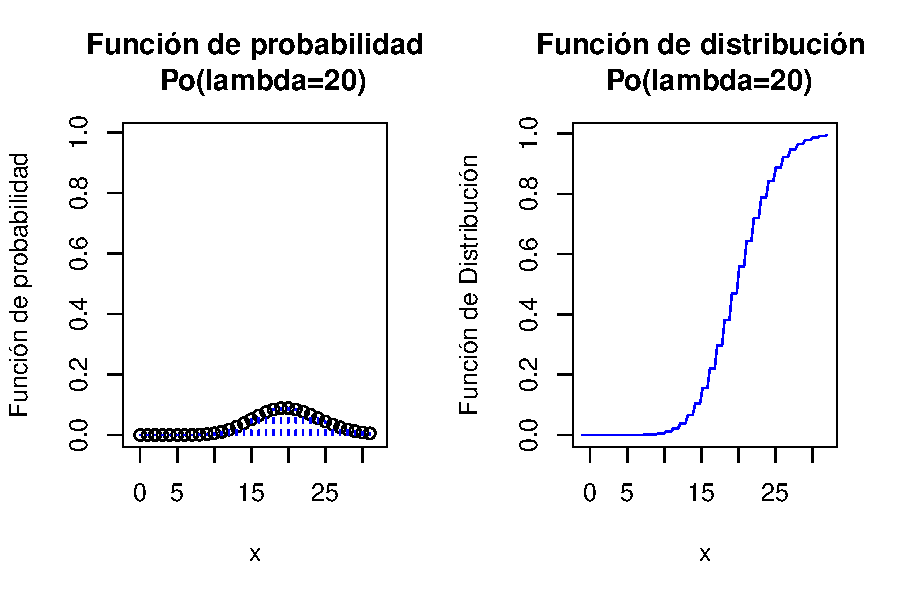
\includegraphics[width=0.7\linewidth,height=\textheight,keepaspectratio]{distibuciones_notables_1_files/figure-pdf/graficosPOISON-1.pdf}
\end{center}

\section{Cálculos con python}\label{cuxe1lculos-con-python-4}

Sea \(X\) un una v.a. \(Po(\lambda=3)\). Entonces

\(P_X(0)=P(X=0), P_X(1)=P(X=1)\) en este orden son

\begin{Shaded}
\begin{Highlighting}[]
\ImportTok{from}\NormalTok{ scipy.stats }\ImportTok{import}\NormalTok{ poisson}
\NormalTok{poisson.pmf(}\DecValTok{0}\NormalTok{,mu }\OperatorTok{=} \DecValTok{3}\NormalTok{)}
\end{Highlighting}
\end{Shaded}

\begin{verbatim}
0.049787068367863944
\end{verbatim}

\begin{Shaded}
\begin{Highlighting}[]
\NormalTok{poisson.pmf(}\DecValTok{1}\NormalTok{,mu }\OperatorTok{=} \DecValTok{3}\NormalTok{)}
\end{Highlighting}
\end{Shaded}

\begin{verbatim}
0.14936120510359185
\end{verbatim}

\section{Cálculos con python}\label{cuxe1lculos-con-python-5}

Sea \(X\) un una v.a. \(Po(\lambda=3)\). Entonces

\(F_X(0)=P(X\leq 0), F_X(1)=P(X\leq 1)\) en este orden son

\begin{Shaded}
\begin{Highlighting}[]
\NormalTok{poisson.cdf(}\DecValTok{0}\NormalTok{,mu }\OperatorTok{=} \DecValTok{3}\NormalTok{)}
\end{Highlighting}
\end{Shaded}

\begin{verbatim}
0.04978706836786395
\end{verbatim}

\begin{Shaded}
\begin{Highlighting}[]
\NormalTok{poisson.cdf(}\DecValTok{1}\NormalTok{,mu }\OperatorTok{=} \DecValTok{3}\NormalTok{)}
\end{Highlighting}
\end{Shaded}

\begin{verbatim}
0.1991482734714558
\end{verbatim}

\begin{Shaded}
\begin{Highlighting}[]
\NormalTok{poisson.pmf(}\DecValTok{0}\NormalTok{,mu }\OperatorTok{=} \DecValTok{3}\NormalTok{)}\OperatorTok{+}\NormalTok{poisson.pmf(}\DecValTok{1}\NormalTok{,mu}\OperatorTok{=} \DecValTok{3}\NormalTok{) }
\end{Highlighting}
\end{Shaded}

\begin{verbatim}
0.1991482734714558
\end{verbatim}

\begin{Shaded}
\begin{Highlighting}[]
\CommentTok{\#\# es igual a poisson.cdf(1,lambda=3)}
\end{Highlighting}
\end{Shaded}

\section{Cálculos con python}\label{cuxe1lculos-con-python-6}

Por ejemplo podemos comprobar que
\(F_X(10)=\displaystyle\sum_{0}^{10} P_X(x)\)

\begin{Shaded}
\begin{Highlighting}[]
\NormalTok{poisson.pmf(}\BuiltInTok{range}\NormalTok{(}\DecValTok{0}\NormalTok{,}\DecValTok{10}\NormalTok{),mu}\OperatorTok{=}\DecValTok{3}\NormalTok{)}
\end{Highlighting}
\end{Shaded}

\begin{verbatim}
array([0.04978707, 0.14936121, 0.22404181, 0.22404181, 0.16803136,
       0.10081881, 0.05040941, 0.02160403, 0.00810151, 0.0027005 ])
\end{verbatim}

\begin{Shaded}
\begin{Highlighting}[]
\BuiltInTok{sum}\NormalTok{(poisson.pmf(}\BuiltInTok{range}\NormalTok{(}\DecValTok{0}\NormalTok{,}\DecValTok{10}\NormalTok{),mu}\OperatorTok{=}\DecValTok{3}\NormalTok{))}
\end{Highlighting}
\end{Shaded}

\begin{verbatim}
0.9988975118698846
\end{verbatim}

\begin{Shaded}
\begin{Highlighting}[]
\NormalTok{poisson.cdf(}\DecValTok{10}\NormalTok{,mu}\OperatorTok{=}\DecValTok{3}\NormalTok{)}
\end{Highlighting}
\end{Shaded}

\begin{verbatim}
0.9997076630493527
\end{verbatim}

\section{Cálculos con python}\label{cuxe1lculos-con-python-7}

En el ejercicio de la trampa para insectos teníamos que \(X\) es una
\(Po(20)\). Responded con python a la preguntas 3 y 4 de este ejercicio

\textbf{Pregunta 3.} Calculad la probabilidad de que en una hora caigan
en la trampa exactamente 21 insectos.

La respuesta a la pregunta 3 es calcular \(P(X=21)\)

\begin{Shaded}
\begin{Highlighting}[]
\NormalTok{poisson.pmf(}\DecValTok{21}\NormalTok{,mu}\OperatorTok{=}\DecValTok{20}\NormalTok{)}
\end{Highlighting}
\end{Shaded}

\begin{verbatim}
0.08460506418293791
\end{verbatim}

\begin{Shaded}
\begin{Highlighting}[]
\CommentTok{\# P(X=21)}
\end{Highlighting}
\end{Shaded}

\section{Cálculos con python}\label{cuxe1lculos-con-python-8}

\textbf{Pregunta 4.} Calculad la probabilidad de que en una hora caigan
en la trampa al menos 6 insectos.

La pregunta 4 nos pide calcular \(P(X\geq 6)=1-P(X\leq 5)\)

\begin{Shaded}
\begin{Highlighting}[]
\DecValTok{1}\OperatorTok{{-}}\NormalTok{poisson.cdf(}\DecValTok{5}\NormalTok{,mu}\OperatorTok{=}\DecValTok{20}\NormalTok{) }
\end{Highlighting}
\end{Shaded}

\begin{verbatim}
0.9999280911594716
\end{verbatim}

\begin{Shaded}
\begin{Highlighting}[]
\CommentTok{\# es 1{-}P(X\textless{}=5)=P(X\textgreater{}=6)}
\end{Highlighting}
\end{Shaded}

\section{Cálculos con python}\label{cuxe1lculos-con-python-9}

Como ya hemos visto con \texttt{scipy.stats} podemos pedir los momentos
de una variable aleatoria \(Po(3)\)

\begin{Shaded}
\begin{Highlighting}[]
\NormalTok{poisson.stats(mu}\OperatorTok{=}\DecValTok{3}\NormalTok{, moments}\OperatorTok{=}\StringTok{\textquotesingle{}mv\textquotesingle{}}\NormalTok{)}
\end{Highlighting}
\end{Shaded}

\begin{verbatim}
(array(3.), array(3.))
\end{verbatim}

Y también generar secuencias de observaciones aleatorias de una
población \(Po(3)\)

\begin{Shaded}
\begin{Highlighting}[]
\NormalTok{poisson.rvs(mu}\OperatorTok{=}\DecValTok{3}\NormalTok{,size}\OperatorTok{=}\DecValTok{40}\NormalTok{)}
\end{Highlighting}
\end{Shaded}

\begin{verbatim}
array([2, 4, 3, 5, 3, 2, 4, 2, 1, 2, 2, 1, 2, 1, 3, 1, 2, 2, 2, 3, 2, 3,
       0, 1, 5, 2, 7, 3, 1, 3, 2, 4, 6, 3, 3, 2, 3, 3, 1, 2], dtype=int64)
\end{verbatim}

\section{Gráficos con python}\label{gruxe1ficos-con-python-2}

\begin{Shaded}
\begin{Highlighting}[]
\ImportTok{from}\NormalTok{ scipy.stats }\ImportTok{import}\NormalTok{ poisson}
\NormalTok{mu }\OperatorTok{=} \DecValTok{10} \CommentTok{\# mu = lambda}
\NormalTok{x }\OperatorTok{=}\NormalTok{ np.arange(poisson.ppf(}\FloatTok{0.01}\NormalTok{, mu),poisson.ppf(}\FloatTok{0.99}\NormalTok{, mu))}
\NormalTok{fig }\OperatorTok{=}\NormalTok{plt.figure(figsize}\OperatorTok{=}\NormalTok{(}\DecValTok{5}\NormalTok{, }\FloatTok{2.7}\NormalTok{))}
\NormalTok{ax }\OperatorTok{=}\NormalTok{ fig.add\_subplot(}\DecValTok{1}\NormalTok{,}\DecValTok{2}\NormalTok{,}\DecValTok{1}\NormalTok{)}
\NormalTok{ax.plot(x, poisson.pmf(x, mu), }\StringTok{\textquotesingle{}bo\textquotesingle{}}\NormalTok{, ms}\OperatorTok{=}\DecValTok{5}\NormalTok{, label}\OperatorTok{=}\StringTok{\textquotesingle{}poisson pmf\textquotesingle{}}\NormalTok{)}
\NormalTok{ax.vlines(x, }\DecValTok{0}\NormalTok{, poisson.pmf(x, mu), colors}\OperatorTok{=}\StringTok{\textquotesingle{}b\textquotesingle{}}\NormalTok{, lw}\OperatorTok{=}\DecValTok{2}\NormalTok{, alpha}\OperatorTok{=}\FloatTok{0.5}\NormalTok{)}
\ControlFlowTok{for}\NormalTok{ tick }\KeywordTok{in}\NormalTok{ ax.xaxis.get\_major\_ticks():}
\NormalTok{  tick.label.set\_fontsize(}\DecValTok{5}\NormalTok{)}
\ControlFlowTok{for}\NormalTok{ tick }\KeywordTok{in}\NormalTok{ ax.yaxis.get\_major\_ticks(): }
\NormalTok{  tick.label.set\_fontsize(}\DecValTok{5}\NormalTok{) }
\end{Highlighting}
\end{Shaded}

\section{Gráficos con python}\label{gruxe1ficos-con-python-3}

\begin{Shaded}
\begin{Highlighting}[]
\NormalTok{ax }\OperatorTok{=}\NormalTok{ fig.add\_subplot(}\DecValTok{1}\NormalTok{,}\DecValTok{2}\NormalTok{,}\DecValTok{2}\NormalTok{)}
\NormalTok{ax.plot(x, poisson.cdf(x, mu), }\StringTok{\textquotesingle{}bo\textquotesingle{}}\NormalTok{, ms}\OperatorTok{=}\DecValTok{5}\NormalTok{, label}\OperatorTok{=}\StringTok{\textquotesingle{}poisson cdf\textquotesingle{}}\NormalTok{)}
\NormalTok{ax.vlines(x, }\DecValTok{0}\NormalTok{, poisson.cdf(x, mu), colors}\OperatorTok{=}\StringTok{\textquotesingle{}b\textquotesingle{}}\NormalTok{, lw}\OperatorTok{=}\DecValTok{2}\NormalTok{, alpha}\OperatorTok{=}\FloatTok{0.5}\NormalTok{)}
\ControlFlowTok{for}\NormalTok{ tick }\KeywordTok{in}\NormalTok{ ax.xaxis.get\_major\_ticks():}
\NormalTok{  tick.label.set\_fontsize(}\DecValTok{5}\NormalTok{)}
\ControlFlowTok{for}\NormalTok{ tick }\KeywordTok{in}\NormalTok{ ax.yaxis.get\_major\_ticks():}
\NormalTok{  tick.label.set\_fontsize(}\DecValTok{5}\NormalTok{)}
\NormalTok{fig.suptitle(}\StringTok{\textquotesingle{}Distribucion de Poisson\textquotesingle{}}\NormalTok{)}
\NormalTok{plt.show()}
\end{Highlighting}
\end{Shaded}

\section{Gráficos con python}\label{gruxe1ficos-con-python-4}

\begin{center}
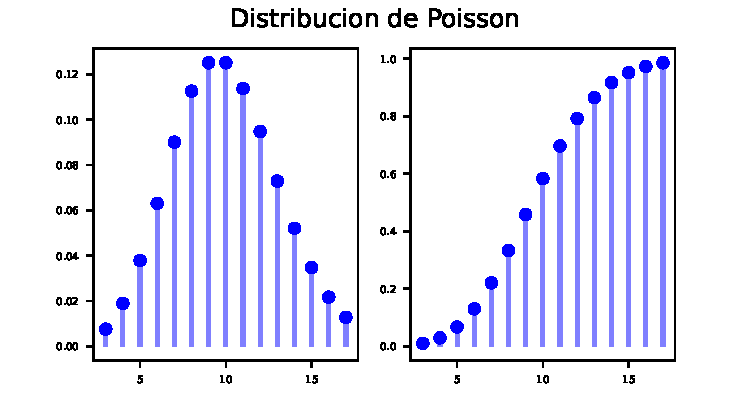
\includegraphics[width=0.7\linewidth,height=\textheight,keepaspectratio]{distibuciones_notables_1_files/figure-pdf/py_poiss2_plot-1.pdf}
\end{center}

\section{Ejemplo proceso Poisson}\label{ejemplo-proceso-poisson}

\textbf{Número de impactos de insectos en la visera de un casco}

Un colega de trabajo, al que llamaremos JG, es muy aficionado a los
grandes premios de velocidad tanto en coches como en motos.

Como es tan aficionado está obsesionado con muchas de las más
extravagantes estadísticas de estos deportes. En particular le
propusimos que estudiara el número de insectos que chocan contra la
visera de un casco de un motorista GP o de un conductor de fórmula 1 .

\section{Ejemplo proceso Poisson}\label{ejemplo-proceso-poisson-1}

La idea es que el número de insectos está igualmente repartido por todo
el circuito y de promedio impactan \(\lambda>0\) insectos por minuto.
También es razonable suponer que:

\begin{itemize}
\tightlist
\item
  podemos dividir la superficie de la visera en cuadrados
  suficientemente pequeños de forma que la probabilidad de que caigan
  dos insectos en la misma zona es prácticamente 0.
\item
  la probabilidad de que un insecto impacte en un cuadrado cualquiera de
  la visera es independiente de cualquier otro cuadrado.
\item
  si hemos dividido la visera en \(n\) cuadrados la probabilidad \(p_n\)
  de impacto de un cuadrado vale \(p_n=\frac{\lambda}{n}\).
\end{itemize}

Bajo estas condiciones, si denotamos por \(X_t\) como el número de
insectos que ha impactado en la visera en el intervalo \((0,t]\) (en
\(t\) minutos), podemos afirmar que \(X_t\) es un proceso de Poisson
\(Po(\lambda\cdot t)\).

\section{Ejemplo proceso Poisson}\label{ejemplo-proceso-poisson-2}

Supongamos que nos dicen que \(\lambda=3\) insectos por minuto. Entonces
el proceso de poisson \(X_t\) seguirá un ley \(Po(3\cdot t).\)

Ahora estamos en condiciones de preguntar al proceso de Poisson.

¿Cuál es la probabilidad de que en 10 minutos impacten más de 25
insectos?

En este caso \(t=10\) \(X_{10}\)= número de insectos que impactan en 10
minutos, el intervalo \([0,10)\) que sigue una \(P(3\cdot 10=30)\). Por
lo tanto

\[P(X>25)=1-P(X\leq 25)\]

lo resolvemos con R

\begin{Shaded}
\begin{Highlighting}[]
\DecValTok{1}\SpecialCharTok{{-}}\FunctionTok{ppois}\NormalTok{(}\DecValTok{25}\NormalTok{,}\AttributeTok{lambda=}\DecValTok{30}\NormalTok{)}
\end{Highlighting}
\end{Shaded}

\begin{verbatim}
[1] 0.7916426
\end{verbatim}

\section{Ejemplo proceso Poisson}\label{ejemplo-proceso-poisson-3}

Otra pregunta interesante es que tengamos que esperar más de 2 minutos
para observar el primer impacto

\[P(X_2=0)=\frac{(3\cdot 2)^0}{0!}\cdot e^{-3\cdot 2}= e^{-6}=0.002479.\]

Con R

\begin{Shaded}
\begin{Highlighting}[]
\DecValTok{6}\SpecialCharTok{\^{}}\DecValTok{0}\SpecialCharTok{/}\FunctionTok{factorial}\NormalTok{(}\DecValTok{0}\NormalTok{)}\SpecialCharTok{*}\FunctionTok{exp}\NormalTok{(}\SpecialCharTok{{-}}\DecValTok{6}\NormalTok{)}
\end{Highlighting}
\end{Shaded}

\begin{verbatim}
[1] 0.002478752
\end{verbatim}

\begin{Shaded}
\begin{Highlighting}[]
\FunctionTok{ppois}\NormalTok{(}\DecValTok{0}\NormalTok{,}\AttributeTok{lambda=}\DecValTok{3}\SpecialCharTok{*}\DecValTok{2}\NormalTok{)}
\end{Highlighting}
\end{Shaded}

\begin{verbatim}
[1] 0.002478752
\end{verbatim}

\chapter{Distribución
hipergeométrica}\label{distribuciuxf3n-hipergeomuxe9trica}

\section{Modelo de la distribución
hipergeométrica}\label{modelo-de-la-distribuciuxf3n-hipergeomuxe9trica}

Supongamos que disponemos de una urna de de sorteos que contiene \(m\)
bolas blancas y \(n\) bolas rojas.

En total en esta urna hay \(m+n\) bolas, \(m\) blancas y \(n\) rojas. Si
extraemos dos bolas de la urna lo podemos hacer de dos formas:

\begin{itemize}
\tightlist
\item
  Extraer una anotar su color y reponerla. Sacar otra y anotar su color.
  Hemos extraído la bola con reposición.
\item
  Extraer simultáneamente dos bolas (sin reposición) y contar el número
  de bolas blancas.
\end{itemize}

\section{Modelo de la distribución
hipergeométrica}\label{modelo-de-la-distribuciuxf3n-hipergeomuxe9trica-1}

Sea \(X\) es la v.a. que cuenta el número de bolas blancas extraídas.

\begin{itemize}
\tightlist
\item
  En el primer caso, \(X\) es una \(B(n=2,p=\frac{m}{m+n})\) ya que
  consiste en repetir dos veces el mismo experimento de Bernoulli.
\item
  En el segundo caso, \(X\) sigue una distribución hipergeométrica que
  estudiaremos en esta sección.
\end{itemize}

\section{Modelo de la distribución
hipergeométrica}\label{modelo-de-la-distribuciuxf3n-hipergeomuxe9trica-2}

Distribución hipergeométrica

Sean \(n\), \(m\) y \(k\) tres número enteros positivos y tales que
\(k<m+n\).

Consideremos una urna que contiene \(m+n\) bolas de las que \(m\) son
blancas y las restantes \(n\) no (son no blancas).

El número total de bolas es \(m+n\). Extraemos de forma aleatoria \(k\)
bolas de la urna sin reemplazarlas.

\section{Modelo de la distribución
hipergeométrica}\label{modelo-de-la-distribuciuxf3n-hipergeomuxe9trica-3}

Sea \(X\) la v.a. que cuenta el número de bolas blancas extraídas.
Diremos que la distribución de \(X\) es hipergeométrica de parámetros
\(m\), \(n\) y \(k\) y la denotaremos por \(H(m,n,k)\).

Su dominio es

\[D_X=\left\{x\in\mathbf{N}\mid \max\{0,k-n\}\leq  x \leq \min\{m,k\}\right\}\]

Para explicarlo, veamos varios ejemplos:

\begin{itemize}
\tightlist
\item
  \(H(m=5,n=2,k=3)\). Tenemos \(m=5\) bolas blancas, \(n=2\) no blancas
  y sacamos \(k=3\) bolas sin reposición.

  \begin{itemize}
  \tightlist
  \item
    En este caso el mínimo de bolas blancas extraídas es \(1=k-n=3-2\),
    ya que sólo hay dos no blancas.
  \item
    En cambio, el máximo si es \(k=3\), ya que tenemos bolas blancas de
    ``sobra''.
  \end{itemize}
\end{itemize}

\section{Modelo de la distribución
hipergeométrica}\label{modelo-de-la-distribuciuxf3n-hipergeomuxe9trica-4}

\[D_X=\left\{x\in\mathbf{N}\mid \max\{0,k-n\}\leq  x \leq \min\{m,k\}\right\}\]

\begin{itemize}
\tightlist
\item
  \(H(m=2,n=5,k=3)\). Tenemos \(m=2\) bolas blancas, \(n=5\) no blancas
  y sacamos \(k=3\) bolas sin reposición.

  \begin{itemize}
  \tightlist
  \item
    En este caso el mínimo de bolas blancas es \(0\) ya que puedo sacar
    3 no blancas.
  \item
    En cambio, el máximo si es \(m=2\), ya que aunque saquemos \(k=3\)
    bolas, al llegar a 2 ya hemos extraído todas las bolas blancas de la
    urna.
  \end{itemize}
\item
  \(H(m=10,n=10,k=3)\). Tenemos \(m=10\) bolas blancas, \(n=10\) no
  blancas y sacamos \(k=3\) bolas sin reposición.

  \begin{itemize}
  \tightlist
  \item
    En este caso podemos obtener desde \(0\) blancas hasta \(k=3\)
    blancas.
  \end{itemize}
\end{itemize}

\section{Modelo de la distribución
hipergeométrica}\label{modelo-de-la-distribuciuxf3n-hipergeomuxe9trica-5}

Su función de probabilidad es:

Su función de probabilidad es: \[
P_{X}(x)=\left\{
\begin{array}{ll}
\frac{\binom{m}{x}\cdot \binom{n}{k-x}}{\binom{m+n}{k}}, & \mbox{ si }
\max\{0,k-n\}\leq x \leq \min\{m,k\}, \mbox { para  } x\in \mathbf{N},\\
0,  & \mbox{en otro caso.}\end{array}\right.
\]

\section{Distribución
hipergeométrica}\label{distribuciuxf3n-hipergeomuxe9trica-1}

\textbf{Observación: otras parametrizaciones}

En ocasiones se parametriza una v.a. hipergeométrica mediante \(N=m+n\),
número total de bolas, \(k\), número de extracciones y \(p\),
probabilidad de extraer una bola blanca.

Así podemos \textbf{parametrizar alternativamente} la distribución
hipergeométrica así

\[H(N,k,p)\mbox{ donde } p=\frac{m}{N}.\]

\section{\texorpdfstring{Resumen distribución Hipergeométrica
\(H(m,n,k)\).}{Resumen distribución Hipergeométrica H(m,n,k).}}\label{resumen-distribuciuxf3n-hipergeomuxe9trica-hmnk.}

\renewcommand{\arraystretch}{1.75}
\begin{table}
\centering
\begin{tabular}{|l|}
\hline\rowcolor{LightBlue}
$X= \left\{\begin{array}{l}
\mbox{número de bolas blancas  en $k$ extracciones}\\
\mbox{sin reposición de una urna con} $m$\\
\mbox{bolas blancas y }$n$ \mbox{ negras.}
\end{array}\right.$;  $H(m,n,k)$
\\\hline
$D_X=\left\{x\in\mathbb{N}\mid \max\{0,k-n\}\leq  x \leq \min\{m,k\}\right\}$\\\hline
$P_X(x)=P(X=x)=\left\{
\begin{array}{ll}
\frac{\binom{m}{x}\cdot \binom{n}{k-x}}{\binom{m+n}{k}}, & \mbox{ si }
\max\{0,k-n\}\leq x \leq \min\{m,k\}, \\
0,  & \mbox{en otro caso.}\end{array}\right.$\\\hline
$F_X(x)=P(X\leq x)$.\\\hline
$E(X)=\frac{k\cdot m}{m+n}$; $Var(X)=k\cdot\frac{m}{m+n}\cdot\left(1-\frac{m}{m+n}\right) \cdot\frac{m+n-k}{m+n-1}$
\\\hline
\end{tabular}
\end{table}

\section{\texorpdfstring{Ejemplo clásico urna \(m=15\) blancas, \(n=10\)
rojas y \(k=3\) extracciones sin
reposición.}{Ejemplo clásico urna m=15 blancas, n=10 rojas y k=3 extracciones sin reposición.}}\label{ejemplo-cluxe1sico-urna-m15-blancas-n10-rojas-y-k3-extracciones-sin-reposiciuxf3n.}

\textbf{Urna con bolas blancas y rojas}

Tenemos una urna con 15 bolas blancas y 10 bolas rojas. Extraemos al
azar tres bolas de la urna sin reposición. Sea \(X\) el número de bolas
\textbf{blancas} extraídas. Bajo esta condiciones, la v.a. \(X\) sigue
una ley de distribución \(H(m=15,n=10,k=3)\).

La función de probabilidad es

\[
P_X(x)=P(X=x)=\left\{
\begin{array}{ll}
\frac{\binom{m}{x}\cdot \binom{n}{k-x}}{\binom{m+n}{k}} & \mbox{ si }
\max\{0,k-n\}\leq x \leq \min\{m,k\} \mbox { para  } x\in \mathbf{N}\\
0  & \mbox{en otro caso}\end{array}\right.,
\]

\[\mbox{sustituyendo }\scriptsize{
P_X(x)=P(X=x)=\left\{
\begin{array}{ll}
\frac{\binom{15}{x}\cdot \binom{10}{3-x}}{\binom{25}{3}} & \mbox{ si }
0\leq x \leq 3 \mbox { para  } x\in \mathbf{N}\\
0  & \mbox{en otro caso}\end{array}\right.
}\]

\section{\texorpdfstring{Ejemplo clásico urna \(m=15\) blancas, \(n=10\)
rojas y \(k=3\) extracciones sin
reposición.}{Ejemplo clásico urna m=15 blancas, n=10 rojas y k=3 extracciones sin reposición.}}\label{ejemplo-cluxe1sico-urna-m15-blancas-n10-rojas-y-k3-extracciones-sin-reposiciuxf3n.-1}

La probabilidad de sacar 2 blancas será

\[
P(X=2)=\frac{\binom{15}{2}\cdot \binom{10}{3-2}}{\binom{25}{3}}
\]

\begin{Shaded}
\begin{Highlighting}[]
\FunctionTok{c}\NormalTok{(}\FunctionTok{choose}\NormalTok{(}\DecValTok{15}\NormalTok{,}\DecValTok{2}\NormalTok{), }\FunctionTok{choose}\NormalTok{(}\DecValTok{10}\NormalTok{,}\DecValTok{1}\NormalTok{), }\FunctionTok{choose}\NormalTok{(}\DecValTok{25}\NormalTok{,}\DecValTok{3}\NormalTok{))}
\end{Highlighting}
\end{Shaded}

\begin{verbatim}
[1]  105   10 2300
\end{verbatim}

\(P(X=2)=\frac{105\cdot10 }{2300}=0.4565217.\)

\section{\texorpdfstring{Ejemplo clásico urna \(m=15\) blancas, \(n=10\)
rojas y \(k=3\) extracciones sin
reposición.}{Ejemplo clásico urna m=15 blancas, n=10 rojas y k=3 extracciones sin reposición.}}\label{ejemplo-cluxe1sico-urna-m15-blancas-n10-rojas-y-k3-extracciones-sin-reposiciuxf3n.-2}

La probabilidad de que saquemos más de 1 bola blanca es

\[
\begin{array}{rl}
P(X> 1)&= 1-P(X\leq 1)=1-(P(X=0)+P(X=1))\\
&=
1-\left(\frac{\binom{15}{0}\cdot \binom{10}{3}}{\binom{25}{3}}+
\frac{\binom{15}{1}\cdot \binom{10}{2}}{\binom{25}{3}}\right)\\
&=
1-\left(
\frac{1\cdot120 }{2300}+\frac{15\cdot45 }{2300}
\right)=1-\frac{120+15\cdot 45}{2300}=0.6543478.
\end{array}
\]

\section{\texorpdfstring{Ejemplo clásico urna \(m=15\) blancas, \(n=10\)
rojas y \(k=3\) extracciones sin
reposición.}{Ejemplo clásico urna m=15 blancas, n=10 rojas y k=3 extracciones sin reposición.}}\label{ejemplo-cluxe1sico-urna-m15-blancas-n10-rojas-y-k3-extracciones-sin-reposiciuxf3n.-3}

El número esperado de bolas blancas extraídas para una v.a. \(X\)
\(H(m=15,n=10,k=3)\) es

\[E(X)=\frac{k\cdot m}{m+n}=\frac{3\cdot 15}{15+10}=\frac{45}{35}=1.285714.\]

La varianza vale: \[
\begin{array}{rl}
Var(X)&=k\cdot\frac{m}{m+n}\cdot\left(1-\frac{m}{m+n}\right) \cdot\frac{m+n-k}{m+n-1}\\
&=3\cdot\frac{15}{15+10}\cdot\left(1-\frac{15}{15+10}\right) \cdot\frac{15+10-3}{15+10-1}\\
&=
3\cdot\frac{15}{25}\cdot\left(1-\frac{15}{25}\right) \cdot\frac{22}{24}= 
3\cdot\frac{15}{25}\cdot\frac{25-15}{25} \cdot\frac{22}{24}\\
&=
3\cdot\frac{15}{25}\cdot\frac{10}{25}\cdot\frac{22}{24}=0.66.
\end{array}
\]

Y por lo tanto su desviación típica es
\(+\sqrt{Var(X)}=+\sqrt{0.66}=0.812404.\)

\section{Cálculos con R}\label{cuxe1lculos-con-r-9}

Sea \(X\) una v.a. \(H(m,n,k)\). La función de \texttt{R} para calcular
la función de probabilidad en un valor \(x\), \(P(X=x)\), es
\texttt{dhyper(x,m,n,k)} y para calcular la función de distribución en
un valor \(q\), \(P(X\leq q)\), es \texttt{phyper(q,m,n,k)}. Para
generar una muestra de valores que siga la distribución \(H(m,n,k)\),
hay que usar la función \texttt{rhyper(nn,m,n,k)} donde \texttt{nn} es
el número de observaciones aleatorias deseado de la muestra.

Por ejemplo, si \(X\) es una \(H(m=15,n=10,k=3)\), los valores de
\(P(X=2)\) y que \(P(X>1)=1-P(X\leq 1)\) son:

\section{Cálculos con R}\label{cuxe1lculos-con-r-10}

\begin{Shaded}
\begin{Highlighting}[]
\FunctionTok{dhyper}\NormalTok{(}\AttributeTok{x=}\DecValTok{2}\NormalTok{,}\AttributeTok{m=}\DecValTok{15}\NormalTok{,}\DecValTok{10}\NormalTok{,}\AttributeTok{k=}\DecValTok{3}\NormalTok{)}
\end{Highlighting}
\end{Shaded}

\begin{verbatim}
[1] 0.4565217
\end{verbatim}

\begin{Shaded}
\begin{Highlighting}[]
\FunctionTok{phyper}\NormalTok{(}\AttributeTok{q=}\DecValTok{1}\NormalTok{,}\AttributeTok{m=}\DecValTok{15}\NormalTok{,}\AttributeTok{n=}\DecValTok{10}\NormalTok{,}\AttributeTok{k=}\DecValTok{3}\NormalTok{)}\CommentTok{\# sí, le han puesto q ya veremos el porqué}
\end{Highlighting}
\end{Shaded}

\begin{verbatim}
[1] 0.3456522
\end{verbatim}

\begin{Shaded}
\begin{Highlighting}[]
\DecValTok{1}\SpecialCharTok{{-}}\FunctionTok{phyper}\NormalTok{(}\AttributeTok{q=}\DecValTok{1}\NormalTok{,}\AttributeTok{m=}\DecValTok{15}\NormalTok{,}\AttributeTok{n=}\DecValTok{10}\NormalTok{,}\AttributeTok{k=}\DecValTok{3}\NormalTok{)}
\end{Highlighting}
\end{Shaded}

\begin{verbatim}
[1] 0.6543478
\end{verbatim}

\section{Cálculos con R}\label{cuxe1lculos-con-r-11}

Una muestra aleatoria de este experimento de tamaño 200 sería:

\begin{Shaded}
\begin{Highlighting}[]
\FunctionTok{rhyper}\NormalTok{(}\AttributeTok{nn=}\DecValTok{200}\NormalTok{,}\AttributeTok{m=}\DecValTok{15}\NormalTok{,}\AttributeTok{n=}\DecValTok{10}\NormalTok{,}\AttributeTok{k=}\DecValTok{3}\NormalTok{)}
\end{Highlighting}
\end{Shaded}

\begin{verbatim}
  [1] 2 3 1 3 1 2 2 3 2 2 1 2 1 2 2 3 3 1 1 1 1 0 2 3 2 1 3 2 2 2 2 3 2 3 3
 [36] 2 0 1 2 1 3 2 2 3 2 3 2 2 3 2 3 1 2 2 2 2 3 2 2 1 3 2 2 3 1 2 2 2 2 2
 [71] 3 0 2 0 3 2 2 2 1 2 2 3 1 1 1 2 2 2 2 1 1 3 2 2 3 2 2 1 1 1 3 3 2 2 2
[106] 1 3 2 2 2 1 1 2 3 2 2 1 2 2 2 2 2 2 3 1 2 3 3 1 1 2 2 1 1 3 2 1 1 2 2
[141] 3 1 1 1 2 1 1 3 1 2 2 3 3 2 3 1 2 1 2 2 2 1 2 3 1 3 3 3 2 2 1 3 3 1 1
[176] 2 2 2 2 2 3 2 1 2 1 1 1 1 2 1 1 2 2 2 2 3 3 1 0 2
\end{verbatim}

\section{Gráficas con R}\label{gruxe1ficas-con-r}

\begin{center}
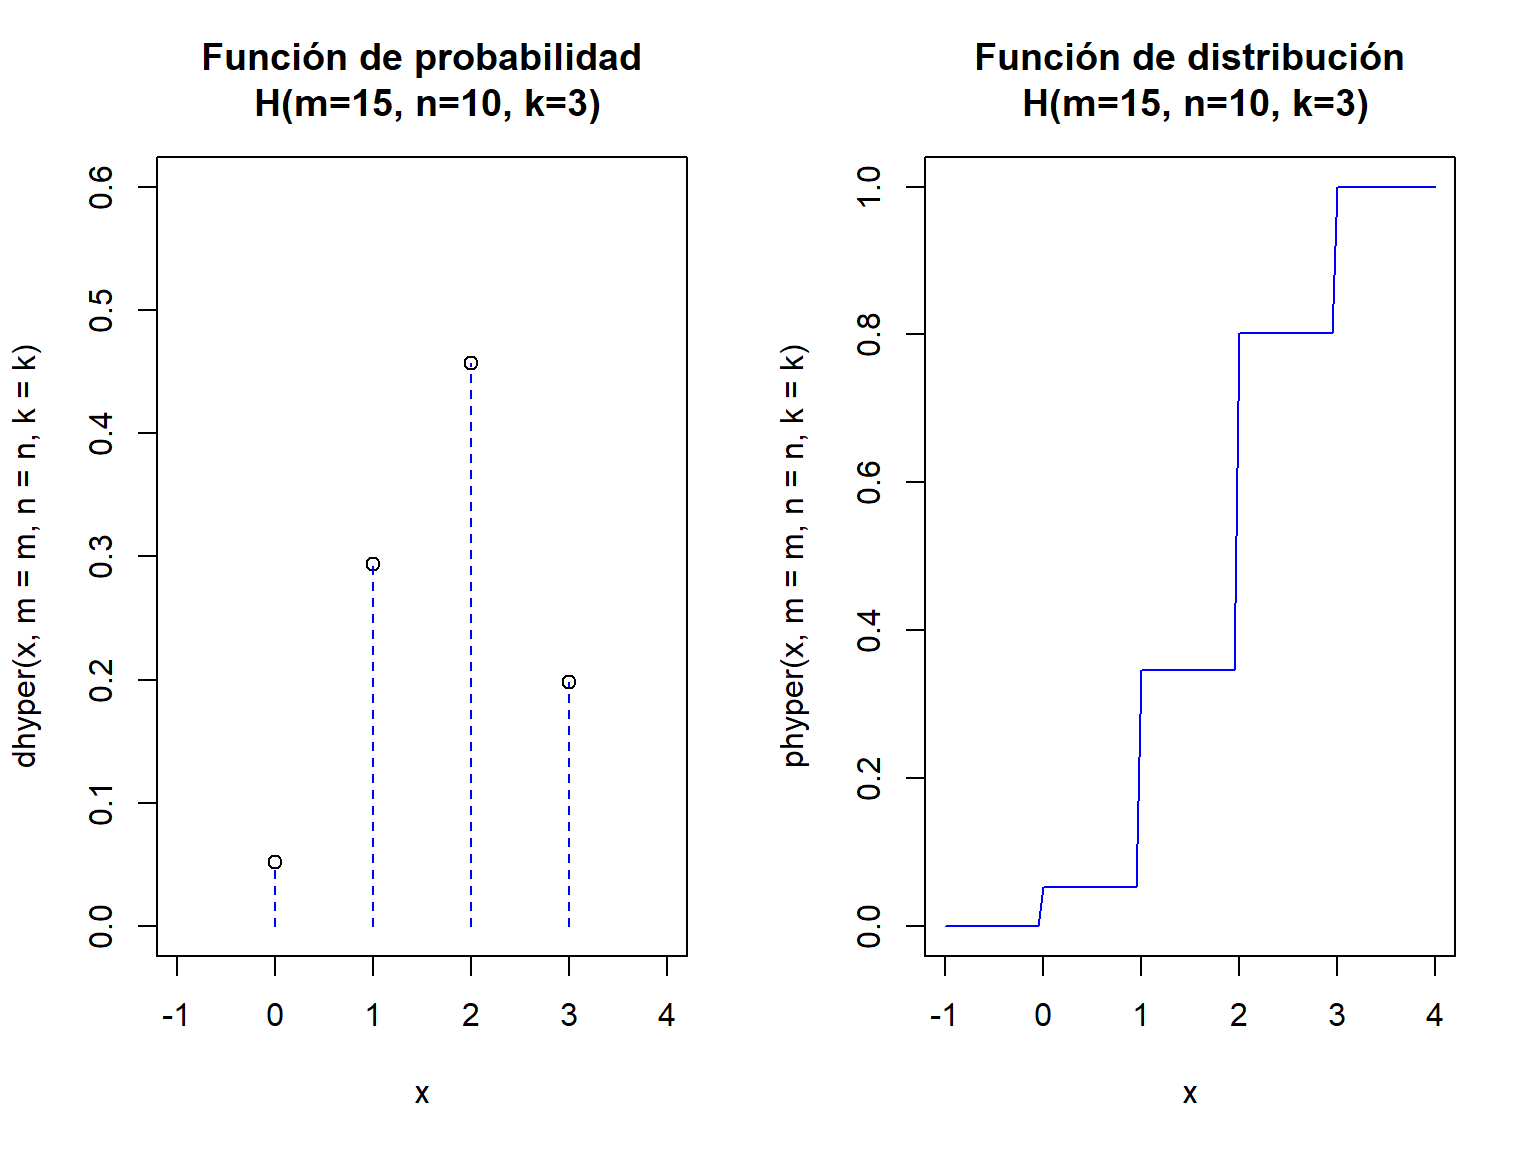
\includegraphics[width=0.7\linewidth,height=\textheight,keepaspectratio]{distibuciones_notables_1_files/figure-pdf/unnamed-chunk-53-1.pdf}
\end{center}

\section{Cálculos con python}\label{cuxe1lculos-con-python-10}

Sea \(X\) una \(H(m,n,k)\), las funciones de \texttt{scipy.stats}
cambian los parámetros

\begin{itemize}
\tightlist
\item
  \(M\) es el número total de bolas. Con nuestra parametrización
  \(M=m+n\).
\item
  \(n\) es el número de bolas blancas. Con nuestra parametrización
  \(n=m\).
\item
  \(N\) es el número de extracciones. Con nuestra parametrización
  \(N=k\).
\end{itemize}

\begin{Shaded}
\begin{Highlighting}[]
\ImportTok{from}\NormalTok{ scipy.stats }\ImportTok{import}\NormalTok{ hypergeom}
\end{Highlighting}
\end{Shaded}

\section{Cálculos con python}\label{cuxe1lculos-con-python-11}

\begin{Shaded}
\begin{Highlighting}[]
\NormalTok{hypergeom.pmf(}\DecValTok{1}\NormalTok{,M}\OperatorTok{=}\DecValTok{15}\OperatorTok{+}\DecValTok{10}\NormalTok{,n}\OperatorTok{=}\DecValTok{15}\NormalTok{,N}\OperatorTok{=}\DecValTok{3}\NormalTok{)}
\end{Highlighting}
\end{Shaded}

\begin{verbatim}
0.2934782608695652
\end{verbatim}

\begin{Shaded}
\begin{Highlighting}[]
\NormalTok{hypergeom.cdf(}\DecValTok{1}\NormalTok{,M}\OperatorTok{=}\DecValTok{15}\OperatorTok{+}\DecValTok{10}\NormalTok{,n}\OperatorTok{=}\DecValTok{15}\NormalTok{,N}\OperatorTok{=}\DecValTok{3}\NormalTok{)}
\end{Highlighting}
\end{Shaded}

\begin{verbatim}
0.3456521739130434
\end{verbatim}

\begin{Shaded}
\begin{Highlighting}[]
\DecValTok{1}\OperatorTok{{-}}\NormalTok{hypergeom.cdf(}\DecValTok{1}\NormalTok{,M}\OperatorTok{=}\DecValTok{15}\OperatorTok{+}\DecValTok{10}\NormalTok{,n}\OperatorTok{=}\DecValTok{15}\NormalTok{,N}\OperatorTok{=}\DecValTok{3}\NormalTok{)}
\end{Highlighting}
\end{Shaded}

\begin{verbatim}
0.6543478260869566
\end{verbatim}

\section{Cálculos con python}\label{cuxe1lculos-con-python-12}

Una muestra aleatoria de este experimento sería\ldots{}

\begin{Shaded}
\begin{Highlighting}[]
\NormalTok{hypergeom.rvs(M}\OperatorTok{=}\DecValTok{15}\OperatorTok{+}\DecValTok{10}\NormalTok{,n}\OperatorTok{=}\DecValTok{15}\NormalTok{,N}\OperatorTok{=}\DecValTok{3}\NormalTok{,size}\OperatorTok{=}\DecValTok{100}\NormalTok{)}
\end{Highlighting}
\end{Shaded}

\begin{verbatim}
array([1, 1, 1, 2, 2, 3, 2, 3, 1, 2, 2, 2, 2, 2, 3, 1, 2, 1, 1, 3, 1, 2,
       2, 2, 1, 1, 1, 2, 1, 2, 3, 1, 2, 2, 2, 3, 0, 3, 2, 1, 2, 1, 1, 2,
       1, 3, 1, 1, 2, 1, 1, 2, 2, 2, 2, 0, 3, 3, 1, 2, 2, 3, 2, 1, 1, 2,
       1, 1, 2, 1, 2, 2, 1, 3, 1, 2, 3, 2, 2, 1, 2, 2, 3, 1, 2, 1, 3, 1,
       1, 1, 3, 1, 2, 2, 2, 2, 1, 2, 1, 3], dtype=int64)
\end{verbatim}

\section{Gráficos con python}\label{gruxe1ficos-con-python-5}

\begin{Shaded}
\begin{Highlighting}[]
\ImportTok{from}\NormalTok{ scipy.stats }\ImportTok{import}\NormalTok{ hypergeom}
\NormalTok{[M, n, N] }\OperatorTok{=}\NormalTok{ [}\DecValTok{20}\NormalTok{, }\DecValTok{7}\NormalTok{, }\DecValTok{12}\NormalTok{] }\CommentTok{\#\#20 elementos, 7 del tipo, extraemos 12}
\NormalTok{x }\OperatorTok{=}\NormalTok{ np.arange(}\BuiltInTok{max}\NormalTok{(}\DecValTok{0}\NormalTok{, N}\OperatorTok{{-}}\NormalTok{M}\OperatorTok{+}\NormalTok{n),}\BuiltInTok{min}\NormalTok{(n, N))}
\NormalTok{fig }\OperatorTok{=}\NormalTok{plt.figure(figsize}\OperatorTok{=}\NormalTok{(}\DecValTok{5}\NormalTok{, }\FloatTok{2.7}\NormalTok{))}
 \OperatorTok{=}\NormalTok{ax }\OperatorTok{=}\NormalTok{ fig.add\_subplot(}\DecValTok{1}\NormalTok{,}\DecValTok{2}\NormalTok{,}\DecValTok{1}\NormalTok{)}
 \OperatorTok{=}\NormalTok{ax.plot(x, hypergeom.pmf(x, M, n, N), }\StringTok{\textquotesingle{}bo\textquotesingle{}}\NormalTok{, ms}\OperatorTok{=}\DecValTok{5}\NormalTok{, label}\OperatorTok{=}\StringTok{\textquotesingle{}hypergeom pmf\textquotesingle{}}\NormalTok{)}
 \OperatorTok{=}\NormalTok{ax.vlines(x, }\DecValTok{0}\NormalTok{, hypergeom.pmf(x, M, n, N), colors}\OperatorTok{=}\StringTok{\textquotesingle{}b\textquotesingle{}}\NormalTok{, lw}\OperatorTok{=}\DecValTok{2}\NormalTok{, alpha}\OperatorTok{=}\FloatTok{0.5}\NormalTok{)}
 \OperatorTok{=}\NormalTok{ax.set\_ylim([}\DecValTok{0}\NormalTok{, }\BuiltInTok{max}\NormalTok{(hypergeom.pmf(x, M, n, N))}\OperatorTok{*}\FloatTok{1.1}\NormalTok{])}
\end{Highlighting}
\end{Shaded}

\section{Gráficos con python}\label{gruxe1ficos-con-python-6}

\begin{Shaded}
\begin{Highlighting}[]
\ControlFlowTok{for}\NormalTok{ tick }\KeywordTok{in}\NormalTok{ ax.xaxis.get\_major\_ticks():}
   \OperatorTok{=}\NormalTok{tick.label.set\_fontsize(}\DecValTok{5}\NormalTok{)}
\ControlFlowTok{for}\NormalTok{ tick }\KeywordTok{in}\NormalTok{ ax.yaxis.get\_major\_ticks():}
  \OperatorTok{=}\NormalTok{tick.label.set\_fontsize(}\DecValTok{5}\NormalTok{) }
\NormalTok{ax }\OperatorTok{=}\NormalTok{ fig.add\_subplot(}\DecValTok{1}\NormalTok{,}\DecValTok{2}\NormalTok{,}\DecValTok{2}\NormalTok{)}
 \OperatorTok{=}\NormalTok{ax.plot(x, hypergeom.cdf(x, M, n, N), }\StringTok{\textquotesingle{}bo\textquotesingle{}}\NormalTok{, ms}\OperatorTok{=}\DecValTok{5}\NormalTok{, label}\OperatorTok{=}\StringTok{\textquotesingle{}hypergeom cdf\textquotesingle{}}\NormalTok{)}
 \OperatorTok{=}\NormalTok{ax.vlines(x, }\DecValTok{0}\NormalTok{, hypergeom.cdf(x, M, n, N), colors}\OperatorTok{=}\StringTok{\textquotesingle{}b\textquotesingle{}}\NormalTok{, lw}\OperatorTok{=}\DecValTok{2}\NormalTok{, alpha}\OperatorTok{=}\FloatTok{0.5}\NormalTok{)}
\ControlFlowTok{for}\NormalTok{ tick }\KeywordTok{in}\NormalTok{ ax.xaxis.get\_major\_ticks():}
   \OperatorTok{=}\NormalTok{tick.label.set\_fontsize(}\DecValTok{5}\NormalTok{)}
\ControlFlowTok{for}\NormalTok{ tick }\KeywordTok{in}\NormalTok{ ax.yaxis.get\_major\_ticks():}
   \OperatorTok{=}\NormalTok{tick.label.set\_fontsize(}\DecValTok{5}\NormalTok{)}
 \OperatorTok{=}\NormalTok{fig.suptitle(}\StringTok{\textquotesingle{}Distribucion Hipergeometrica\textquotesingle{}}\NormalTok{)}
 \OperatorTok{=}\NormalTok{plt.show()}
\end{Highlighting}
\end{Shaded}

\section{Gráficos con python}\label{gruxe1ficos-con-python-7}

\begin{center}
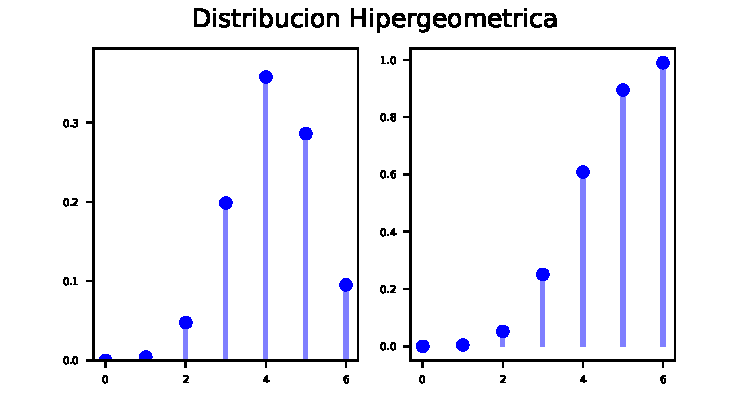
\includegraphics[width=0.7\linewidth,height=\textheight,keepaspectratio]{distibuciones_notables_1_files/figure-pdf/py_hyper2-1.pdf}
\end{center}

\chapter{Distribuciones notables 2}\label{distribuciones-notables-2}




\end{document}
